\documentclass[a4paper]{book}
\usepackage{makeidx}
\usepackage{natbib}
\usepackage{graphicx}
\usepackage{multicol}
\usepackage{float}
\usepackage{listings}
\usepackage{color}
\usepackage{ifthen}
\usepackage[table]{xcolor}
\usepackage{textcomp}
\usepackage{alltt}
\usepackage{ifpdf}
\ifpdf
\usepackage[pdftex,
            pagebackref=true,
            colorlinks=true,
            linkcolor=blue,
            unicode
           ]{hyperref}
\else
\usepackage[ps2pdf,
            pagebackref=true,
            colorlinks=true,
            linkcolor=blue,
            unicode
           ]{hyperref}
\usepackage{pspicture}
\fi
\usepackage[utf8]{inputenc}
\usepackage{mathptmx}
\usepackage[scaled=.90]{helvet}
\usepackage{courier}
\usepackage{sectsty}
\usepackage[titles]{tocloft}
\usepackage{doxygen}
\lstset{language=C++,inputencoding=utf8,basicstyle=\footnotesize,breaklines=true,breakatwhitespace=true,tabsize=8,numbers=left }
\makeindex
\setcounter{tocdepth}{3}
\renewcommand{\footrulewidth}{0.4pt}
\renewcommand{\familydefault}{\sfdefault}
\hfuzz=15pt
\setlength{\emergencystretch}{15pt}
\hbadness=750
\tolerance=750
\begin{document}
\hypersetup{pageanchor=false,citecolor=blue}
\begin{titlepage}
\vspace*{7cm}
\begin{center}
{\Large mcpele \\[1ex]\large 1.\-0.\-0 }\\
\vspace*{1cm}
{\large \-Generated by Doxygen 1.7.6.1}\\
\vspace*{0.5cm}
{\small Wed Dec 10 2014 12:57:10}\\
\end{center}
\end{titlepage}
\clearemptydoublepage
\pagenumbering{roman}
\tableofcontents
\clearemptydoublepage
\pagenumbering{arabic}
\hypersetup{pageanchor=true,citecolor=blue}
\chapter{\-Namespace \-Index}
\section{\-Namespace \-List}
\-Here is a list of all namespaces with brief descriptions\-:\begin{DoxyCompactList}
\item\contentsline{section}{\hyperlink{namespacemcpele}{mcpele} }{\pageref{namespacemcpele}}{}
\end{DoxyCompactList}

\chapter{\-Class \-Index}
\section{\-Class \-Hierarchy}
\-This inheritance list is sorted roughly, but not completely, alphabetically\-:\begin{DoxyCompactList}
\item \contentsline{section}{mcpele\-:\-:\-Accept\-Test}{\pageref{classmcpele_1_1AcceptTest}}{}
\begin{DoxyCompactList}
\item \contentsline{section}{mcpele\-:\-:\-Energy\-Window\-Test}{\pageref{classmcpele_1_1EnergyWindowTest}}{}
\item \contentsline{section}{mcpele\-:\-:\-Metropolis\-Test}{\pageref{classmcpele_1_1MetropolisTest}}{}
\end{DoxyCompactList}
\item \contentsline{section}{mcpele\-:\-:\-Action}{\pageref{classmcpele_1_1Action}}{}
\begin{DoxyCompactList}
\item \contentsline{section}{mcpele\-:\-:\-Record\-Energy\-Histogram}{\pageref{classmcpele_1_1RecordEnergyHistogram}}{}
\item \contentsline{section}{mcpele\-:\-:\-Record\-Pair\-Dist\-Histogram$<$ \-B\-O\-X\-D\-I\-M $>$}{\pageref{classmcpele_1_1RecordPairDistHistogram}}{}
\item \contentsline{section}{mcpele\-:\-:\-Record\-Scalar\-Timeseries}{\pageref{classmcpele_1_1RecordScalarTimeseries}}{}
\begin{DoxyCompactList}
\item \contentsline{section}{mcpele\-:\-:\-Record\-Displacement\-Per\-Particle\-Timeseries}{\pageref{classmcpele_1_1RecordDisplacementPerParticleTimeseries}}{}
\item \contentsline{section}{mcpele\-:\-:\-Record\-Energy\-Timeseries}{\pageref{classmcpele_1_1RecordEnergyTimeseries}}{}
\item \contentsline{section}{mcpele\-:\-:\-Record\-Lowest\-E\-Value\-Timeseries}{\pageref{classmcpele_1_1RecordLowestEValueTimeseries}}{}
\end{DoxyCompactList}
\end{DoxyCompactList}
\item \contentsline{section}{mcpele\-:\-:\-Conf\-Test}{\pageref{classmcpele_1_1ConfTest}}{}
\begin{DoxyCompactList}
\item \contentsline{section}{mcpele\-:\-:\-Check\-Spherical\-Container}{\pageref{classmcpele_1_1CheckSphericalContainer}}{}
\end{DoxyCompactList}
\item \contentsline{section}{mcpele\-:\-:\-Find\-Lowest\-Eigenvalue}{\pageref{classmcpele_1_1FindLowestEigenvalue}}{}
\item \contentsline{section}{mcpele\-:\-:\-Get\-Displacement\-Per\-Particle}{\pageref{classmcpele_1_1GetDisplacementPerParticle}}{}
\item \contentsline{section}{mcpele\-:\-:\-Histogram}{\pageref{classmcpele_1_1Histogram}}{}
\item \contentsline{section}{mcpele\-:\-:\-M\-C}{\pageref{classmcpele_1_1MC}}{}
\item \contentsline{section}{mcpele\-:\-:\-Moments}{\pageref{classmcpele_1_1Moments}}{}
\item \contentsline{section}{mcpele\-:\-:\-Moving\-Average\-Acc}{\pageref{classmcpele_1_1MovingAverageAcc}}{}
\item \contentsline{section}{mcpele\-:\-:\-Pair\-Dist\-Histogram$<$ \-B\-O\-X\-D\-I\-M $>$}{\pageref{classmcpele_1_1PairDistHistogram}}{}
\item \contentsline{section}{mcpele\-:\-:\-Pattern\-Manager$<$ \-T $>$}{\pageref{classmcpele_1_1PatternManager}}{}
\item \contentsline{section}{mcpele\-:\-:progress}{\pageref{classmcpele_1_1progress}}{}
\item \contentsline{section}{mcpele\-:\-:\-Take\-Step}{\pageref{classmcpele_1_1TakeStep}}{}
\begin{DoxyCompactList}
\item \contentsline{section}{mcpele\-:\-:\-Adaptive\-Take\-Step}{\pageref{classmcpele_1_1AdaptiveTakeStep}}{}
\item \contentsline{section}{mcpele\-:\-:\-Gaussian\-Coords\-Displacement}{\pageref{classmcpele_1_1GaussianCoordsDisplacement}}{}
\item \contentsline{section}{mcpele\-:\-:\-Particle\-Pair\-Swap}{\pageref{classmcpele_1_1ParticlePairSwap}}{}
\item \contentsline{section}{mcpele\-:\-:\-Random\-Coords\-Displacement}{\pageref{classmcpele_1_1RandomCoordsDisplacement}}{}
\begin{DoxyCompactList}
\item \contentsline{section}{mcpele\-:\-:\-Random\-Coords\-Displacement\-All}{\pageref{classmcpele_1_1RandomCoordsDisplacementAll}}{}
\item \contentsline{section}{mcpele\-:\-:\-Random\-Coords\-Displacement\-Single}{\pageref{classmcpele_1_1RandomCoordsDisplacementSingle}}{}
\end{DoxyCompactList}
\item \contentsline{section}{mcpele\-:\-:\-Take\-Step\-Pattern}{\pageref{classmcpele_1_1TakeStepPattern}}{}
\item \contentsline{section}{mcpele\-:\-:\-Take\-Step\-Probabilities}{\pageref{classmcpele_1_1TakeStepProbabilities}}{}
\end{DoxyCompactList}
\end{DoxyCompactList}

\chapter{\-Class \-Index}
\section{\-Class \-List}
\-Here are the classes, structs, unions and interfaces with brief descriptions\-:\begin{DoxyCompactList}
\item\contentsline{section}{\hyperlink{classmcpele_1_1AcceptTest}{mcpele\-::\-Accept\-Test} }{\pageref{classmcpele_1_1AcceptTest}}{}
\item\contentsline{section}{\hyperlink{classmcpele_1_1Action}{mcpele\-::\-Action} }{\pageref{classmcpele_1_1Action}}{}
\item\contentsline{section}{\hyperlink{classmcpele_1_1AdaptiveTakeStep}{mcpele\-::\-Adaptive\-Take\-Step} }{\pageref{classmcpele_1_1AdaptiveTakeStep}}{}
\item\contentsline{section}{\hyperlink{classmcpele_1_1CheckSphericalContainer}{mcpele\-::\-Check\-Spherical\-Container} }{\pageref{classmcpele_1_1CheckSphericalContainer}}{}
\item\contentsline{section}{\hyperlink{classmcpele_1_1ConfTest}{mcpele\-::\-Conf\-Test} }{\pageref{classmcpele_1_1ConfTest}}{}
\item\contentsline{section}{\hyperlink{classmcpele_1_1EnergyWindowTest}{mcpele\-::\-Energy\-Window\-Test} }{\pageref{classmcpele_1_1EnergyWindowTest}}{}
\item\contentsline{section}{\hyperlink{classmcpele_1_1FindLowestEigenvalue}{mcpele\-::\-Find\-Lowest\-Eigenvalue} }{\pageref{classmcpele_1_1FindLowestEigenvalue}}{}
\item\contentsline{section}{\hyperlink{classmcpele_1_1GaussianCoordsDisplacement}{mcpele\-::\-Gaussian\-Coords\-Displacement} }{\pageref{classmcpele_1_1GaussianCoordsDisplacement}}{}
\item\contentsline{section}{\hyperlink{classmcpele_1_1GetDisplacementPerParticle}{mcpele\-::\-Get\-Displacement\-Per\-Particle} }{\pageref{classmcpele_1_1GetDisplacementPerParticle}}{}
\item\contentsline{section}{\hyperlink{classmcpele_1_1Histogram}{mcpele\-::\-Histogram} }{\pageref{classmcpele_1_1Histogram}}{}
\item\contentsline{section}{\hyperlink{classmcpele_1_1MC}{mcpele\-::\-M\-C} }{\pageref{classmcpele_1_1MC}}{}
\item\contentsline{section}{\hyperlink{classmcpele_1_1MetropolisTest}{mcpele\-::\-Metropolis\-Test} }{\pageref{classmcpele_1_1MetropolisTest}}{}
\item\contentsline{section}{\hyperlink{classmcpele_1_1Moments}{mcpele\-::\-Moments} }{\pageref{classmcpele_1_1Moments}}{}
\item\contentsline{section}{\hyperlink{classmcpele_1_1MovingAverageAcc}{mcpele\-::\-Moving\-Average\-Acc} }{\pageref{classmcpele_1_1MovingAverageAcc}}{}
\item\contentsline{section}{\hyperlink{classmcpele_1_1PairDistHistogram}{mcpele\-::\-Pair\-Dist\-Histogram$<$ B\-O\-X\-D\-I\-M $>$} }{\pageref{classmcpele_1_1PairDistHistogram}}{}
\item\contentsline{section}{\hyperlink{classmcpele_1_1ParticlePairSwap}{mcpele\-::\-Particle\-Pair\-Swap} }{\pageref{classmcpele_1_1ParticlePairSwap}}{}
\item\contentsline{section}{\hyperlink{classmcpele_1_1PatternManager}{mcpele\-::\-Pattern\-Manager$<$ T $>$} }{\pageref{classmcpele_1_1PatternManager}}{}
\item\contentsline{section}{\hyperlink{classmcpele_1_1progress}{mcpele\-::progress} }{\pageref{classmcpele_1_1progress}}{}
\item\contentsline{section}{\hyperlink{classmcpele_1_1RandomCoordsDisplacement}{mcpele\-::\-Random\-Coords\-Displacement} }{\pageref{classmcpele_1_1RandomCoordsDisplacement}}{}
\item\contentsline{section}{\hyperlink{classmcpele_1_1RandomCoordsDisplacementAll}{mcpele\-::\-Random\-Coords\-Displacement\-All} }{\pageref{classmcpele_1_1RandomCoordsDisplacementAll}}{}
\item\contentsline{section}{\hyperlink{classmcpele_1_1RandomCoordsDisplacementSingle}{mcpele\-::\-Random\-Coords\-Displacement\-Single} }{\pageref{classmcpele_1_1RandomCoordsDisplacementSingle}}{}
\item\contentsline{section}{\hyperlink{classmcpele_1_1RecordDisplacementPerParticleTimeseries}{mcpele\-::\-Record\-Displacement\-Per\-Particle\-Timeseries} }{\pageref{classmcpele_1_1RecordDisplacementPerParticleTimeseries}}{}
\item\contentsline{section}{\hyperlink{classmcpele_1_1RecordEnergyHistogram}{mcpele\-::\-Record\-Energy\-Histogram} }{\pageref{classmcpele_1_1RecordEnergyHistogram}}{}
\item\contentsline{section}{\hyperlink{classmcpele_1_1RecordEnergyTimeseries}{mcpele\-::\-Record\-Energy\-Timeseries} }{\pageref{classmcpele_1_1RecordEnergyTimeseries}}{}
\item\contentsline{section}{\hyperlink{classmcpele_1_1RecordLowestEValueTimeseries}{mcpele\-::\-Record\-Lowest\-E\-Value\-Timeseries} }{\pageref{classmcpele_1_1RecordLowestEValueTimeseries}}{}
\item\contentsline{section}{\hyperlink{classmcpele_1_1RecordPairDistHistogram}{mcpele\-::\-Record\-Pair\-Dist\-Histogram$<$ B\-O\-X\-D\-I\-M $>$} }{\pageref{classmcpele_1_1RecordPairDistHistogram}}{}
\item\contentsline{section}{\hyperlink{classmcpele_1_1RecordScalarTimeseries}{mcpele\-::\-Record\-Scalar\-Timeseries} }{\pageref{classmcpele_1_1RecordScalarTimeseries}}{}
\item\contentsline{section}{\hyperlink{classmcpele_1_1TakeStep}{mcpele\-::\-Take\-Step} }{\pageref{classmcpele_1_1TakeStep}}{}
\item\contentsline{section}{\hyperlink{classmcpele_1_1TakeStepPattern}{mcpele\-::\-Take\-Step\-Pattern} }{\pageref{classmcpele_1_1TakeStepPattern}}{}
\item\contentsline{section}{\hyperlink{classmcpele_1_1TakeStepProbabilities}{mcpele\-::\-Take\-Step\-Probabilities} }{\pageref{classmcpele_1_1TakeStepProbabilities}}{}
\end{DoxyCompactList}

\chapter{\-File \-Index}
\section{\-File \-List}
\-Here is a list of all files with brief descriptions\-:\begin{DoxyCompactList}
\item\contentsline{section}{\hyperlink{adaptive__takestep_8cpp}{adaptive\-\_\-takestep.\-cpp} }{\pageref{adaptive__takestep_8cpp}}{}
\item\contentsline{section}{\hyperlink{check__spherical__container_8cpp}{check\-\_\-spherical\-\_\-container.\-cpp} }{\pageref{check__spherical__container_8cpp}}{}
\item\contentsline{section}{\hyperlink{energy__window__test_8cpp}{energy\-\_\-window\-\_\-test.\-cpp} }{\pageref{energy__window__test_8cpp}}{}
\item\contentsline{section}{\hyperlink{gaussian__coords__displacement_8cpp}{gaussian\-\_\-coords\-\_\-displacement.\-cpp} }{\pageref{gaussian__coords__displacement_8cpp}}{}
\item\contentsline{section}{\hyperlink{histogram_8cpp}{histogram.\-cpp} }{\pageref{histogram_8cpp}}{}
\item\contentsline{section}{\hyperlink{lowest__eigenvalue_8cpp}{lowest\-\_\-eigenvalue.\-cpp} }{\pageref{lowest__eigenvalue_8cpp}}{}
\item\contentsline{section}{\hyperlink{mc_8cpp}{mc.\-cpp} }{\pageref{mc_8cpp}}{}
\item\contentsline{section}{\hyperlink{metropolis__test_8cpp}{metropolis\-\_\-test.\-cpp} }{\pageref{metropolis__test_8cpp}}{}
\item\contentsline{section}{\hyperlink{particle__pair__swap_8cpp}{particle\-\_\-pair\-\_\-swap.\-cpp} }{\pageref{particle__pair__swap_8cpp}}{}
\item\contentsline{section}{\hyperlink{random__coords__displacement_8cpp}{random\-\_\-coords\-\_\-displacement.\-cpp} }{\pageref{random__coords__displacement_8cpp}}{}
\item\contentsline{section}{\hyperlink{record__energy__histogram_8cpp}{record\-\_\-energy\-\_\-histogram.\-cpp} }{\pageref{record__energy__histogram_8cpp}}{}
\item\contentsline{section}{\hyperlink{record__scalar__timeseries_8cpp}{record\-\_\-scalar\-\_\-timeseries.\-cpp} }{\pageref{record__scalar__timeseries_8cpp}}{}
\item\contentsline{section}{\hyperlink{rsm__displacement_8cpp}{rsm\-\_\-displacement.\-cpp} }{\pageref{rsm__displacement_8cpp}}{}
\item\contentsline{section}{\hyperlink{take__step__pattern_8cpp}{take\-\_\-step\-\_\-pattern.\-cpp} }{\pageref{take__step__pattern_8cpp}}{}
\item\contentsline{section}{\hyperlink{take__step__probabilities_8cpp}{take\-\_\-step\-\_\-probabilities.\-cpp} }{\pageref{take__step__probabilities_8cpp}}{}
\item\contentsline{section}{mcpele/\hyperlink{adaptive__takestep_8h}{adaptive\-\_\-takestep.\-h} }{\pageref{adaptive__takestep_8h}}{}
\item\contentsline{section}{mcpele/\hyperlink{check__spherical__container_8h}{check\-\_\-spherical\-\_\-container.\-h} }{\pageref{check__spherical__container_8h}}{}
\item\contentsline{section}{mcpele/\hyperlink{energy__window__test_8h}{energy\-\_\-window\-\_\-test.\-h} }{\pageref{energy__window__test_8h}}{}
\item\contentsline{section}{mcpele/\hyperlink{gaussian__coords__displacement_8h}{gaussian\-\_\-coords\-\_\-displacement.\-h} }{\pageref{gaussian__coords__displacement_8h}}{}
\item\contentsline{section}{mcpele/\hyperlink{histogram_8h}{histogram.\-h} }{\pageref{histogram_8h}}{}
\item\contentsline{section}{mcpele/\hyperlink{lowest__eigenvalue_8h}{lowest\-\_\-eigenvalue.\-h} }{\pageref{lowest__eigenvalue_8h}}{}
\item\contentsline{section}{mcpele/\hyperlink{mc_8h}{mc.\-h} }{\pageref{mc_8h}}{}
\item\contentsline{section}{mcpele/\hyperlink{metropolis__test_8h}{metropolis\-\_\-test.\-h} }{\pageref{metropolis__test_8h}}{}
\item\contentsline{section}{mcpele/\hyperlink{moving__average_8h}{moving\-\_\-average.\-h} }{\pageref{moving__average_8h}}{}
\item\contentsline{section}{mcpele/\hyperlink{pair__dist__histogram_8h}{pair\-\_\-dist\-\_\-histogram.\-h} }{\pageref{pair__dist__histogram_8h}}{}
\item\contentsline{section}{mcpele/\hyperlink{particle__pair__swap_8h}{particle\-\_\-pair\-\_\-swap.\-h} }{\pageref{particle__pair__swap_8h}}{}
\item\contentsline{section}{mcpele/\hyperlink{pattern__manager_8h}{pattern\-\_\-manager.\-h} }{\pageref{pattern__manager_8h}}{}
\item\contentsline{section}{mcpele/\hyperlink{progress_8h}{progress.\-h} }{\pageref{progress_8h}}{}
\item\contentsline{section}{mcpele/\hyperlink{random__coords__displacement_8h}{random\-\_\-coords\-\_\-displacement.\-h} }{\pageref{random__coords__displacement_8h}}{}
\item\contentsline{section}{mcpele/\hyperlink{record__displacement__per__particle__timeseries_8h}{record\-\_\-displacement\-\_\-per\-\_\-particle\-\_\-timeseries.\-h} }{\pageref{record__displacement__per__particle__timeseries_8h}}{}
\item\contentsline{section}{mcpele/\hyperlink{record__energy__histogram_8h}{record\-\_\-energy\-\_\-histogram.\-h} }{\pageref{record__energy__histogram_8h}}{}
\item\contentsline{section}{mcpele/\hyperlink{record__energy__timeseries_8h}{record\-\_\-energy\-\_\-timeseries.\-h} }{\pageref{record__energy__timeseries_8h}}{}
\item\contentsline{section}{mcpele/\hyperlink{record__lowest__evalue__timeseries_8h}{record\-\_\-lowest\-\_\-evalue\-\_\-timeseries.\-h} }{\pageref{record__lowest__evalue__timeseries_8h}}{}
\item\contentsline{section}{mcpele/\hyperlink{record__pair__dist__histogram_8h}{record\-\_\-pair\-\_\-dist\-\_\-histogram.\-h} }{\pageref{record__pair__dist__histogram_8h}}{}
\item\contentsline{section}{mcpele/\hyperlink{record__scalar__timeseries_8h}{record\-\_\-scalar\-\_\-timeseries.\-h} }{\pageref{record__scalar__timeseries_8h}}{}
\item\contentsline{section}{mcpele/\hyperlink{rsm__displacement_8h}{rsm\-\_\-displacement.\-h} }{\pageref{rsm__displacement_8h}}{}
\item\contentsline{section}{mcpele/\hyperlink{take__step__pattern_8h}{take\-\_\-step\-\_\-pattern.\-h} }{\pageref{take__step__pattern_8h}}{}
\item\contentsline{section}{mcpele/\hyperlink{take__step__probabilities_8h}{take\-\_\-step\-\_\-probabilities.\-h} }{\pageref{take__step__probabilities_8h}}{}
\end{DoxyCompactList}

\chapter{\-Namespace \-Documentation}
\hypertarget{namespacemcpele}{\section{mcpele \-Namespace \-Reference}
\label{namespacemcpele}\index{mcpele@{mcpele}}
}
\subsection*{\-Classes}
\begin{DoxyCompactItemize}
\item 
class \hyperlink{classmcpele_1_1AdaptiveTakeStep}{\-Adaptive\-Take\-Step}
\item 
class \hyperlink{classmcpele_1_1CheckSphericalContainer}{\-Check\-Spherical\-Container}
\item 
class \hyperlink{classmcpele_1_1EnergyWindowTest}{\-Energy\-Window\-Test}
\item 
class \hyperlink{classmcpele_1_1GaussianCoordsDisplacement}{\-Gaussian\-Coords\-Displacement}
\item 
class \hyperlink{classmcpele_1_1Moments}{\-Moments}
\item 
class \hyperlink{classmcpele_1_1Histogram}{\-Histogram}
\item 
class \hyperlink{classmcpele_1_1FindLowestEigenvalue}{\-Find\-Lowest\-Eigenvalue}
\item 
class \hyperlink{classmcpele_1_1Action}{\-Action}
\item 
class \hyperlink{classmcpele_1_1AcceptTest}{\-Accept\-Test}
\item 
class \hyperlink{classmcpele_1_1ConfTest}{\-Conf\-Test}
\item 
class \hyperlink{classmcpele_1_1TakeStep}{\-Take\-Step}
\item 
class \hyperlink{classmcpele_1_1MC}{\-M\-C}
\item 
class \hyperlink{classmcpele_1_1MetropolisTest}{\-Metropolis\-Test}
\item 
class \hyperlink{classmcpele_1_1MovingAverageAcc}{\-Moving\-Average\-Acc}
\item 
class \hyperlink{classmcpele_1_1PairDistHistogram}{\-Pair\-Dist\-Histogram}
\item 
class \hyperlink{classmcpele_1_1ParticlePairSwap}{\-Particle\-Pair\-Swap}
\item 
class \hyperlink{classmcpele_1_1PatternManager}{\-Pattern\-Manager}
\item 
class \hyperlink{classmcpele_1_1progress}{progress}
\item 
class \hyperlink{classmcpele_1_1RandomCoordsDisplacement}{\-Random\-Coords\-Displacement}
\item 
class \hyperlink{classmcpele_1_1RandomCoordsDisplacementAll}{\-Random\-Coords\-Displacement\-All}
\item 
class \hyperlink{classmcpele_1_1RandomCoordsDisplacementSingle}{\-Random\-Coords\-Displacement\-Single}
\item 
class \hyperlink{classmcpele_1_1RecordDisplacementPerParticleTimeseries}{\-Record\-Displacement\-Per\-Particle\-Timeseries}
\item 
class \hyperlink{classmcpele_1_1RecordEnergyHistogram}{\-Record\-Energy\-Histogram}
\item 
class \hyperlink{classmcpele_1_1RecordEnergyTimeseries}{\-Record\-Energy\-Timeseries}
\item 
class \hyperlink{classmcpele_1_1RecordLowestEValueTimeseries}{\-Record\-Lowest\-E\-Value\-Timeseries}
\item 
class \hyperlink{classmcpele_1_1RecordPairDistHistogram}{\-Record\-Pair\-Dist\-Histogram}
\item 
class \hyperlink{classmcpele_1_1RecordScalarTimeseries}{\-Record\-Scalar\-Timeseries}
\item 
class \hyperlink{classmcpele_1_1GetDisplacementPerParticle}{\-Get\-Displacement\-Per\-Particle}
\item 
class \hyperlink{classmcpele_1_1TakeStepPattern}{\-Take\-Step\-Pattern}
\item 
class \hyperlink{classmcpele_1_1TakeStepProbabilities}{\-Take\-Step\-Probabilities}
\end{DoxyCompactItemize}

\chapter{\-Class \-Documentation}
\hypertarget{classmcpele_1_1AcceptTest}{\section{mcpele\-:\-:\-Accept\-Test \-Class \-Reference}
\label{classmcpele_1_1AcceptTest}\index{mcpele\-::\-Accept\-Test@{mcpele\-::\-Accept\-Test}}
}


{\ttfamily \#include $<$mc.\-h$>$}

\-Inheritance diagram for mcpele\-:\-:\-Accept\-Test\-:\begin{figure}[H]
\begin{center}
\leavevmode
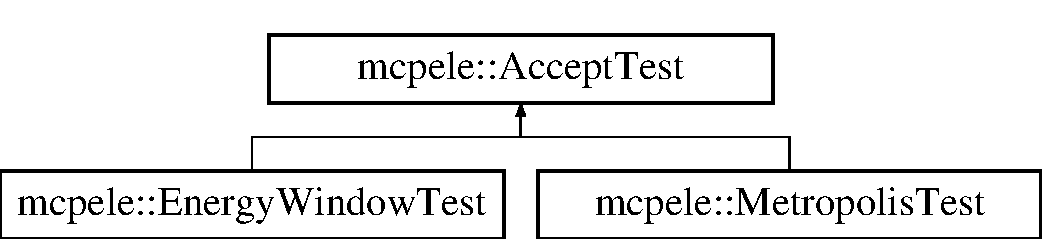
\includegraphics[height=2.000000cm]{classmcpele_1_1AcceptTest}
\end{center}
\end{figure}
\subsection*{\-Public \-Member \-Functions}
\begin{DoxyCompactItemize}
\item 
virtual \hyperlink{classmcpele_1_1AcceptTest_ab2a9fd77376ce15e1c7c5b1ee0df23fc}{$\sim$\-Accept\-Test} ()
\item 
virtual bool \hyperlink{classmcpele_1_1AcceptTest_ae2d9e2feaae60d49a35c7170f56f5d78}{test} (pele\-::\-Array$<$ double $>$ \&trial\-\_\-coords, double trial\-\_\-energy, pele\-::\-Array$<$ double $>$ \&old\-\_\-coords, double old\-\_\-energy, double temperature, \hyperlink{classmcpele_1_1MC}{\-M\-C} $\ast$mc)=0
\end{DoxyCompactItemize}


\subsection{\-Detailed \-Description}


\-Definition at line 33 of file mc.\-h.



\subsection{\-Constructor \& \-Destructor \-Documentation}
\hypertarget{classmcpele_1_1AcceptTest_ab2a9fd77376ce15e1c7c5b1ee0df23fc}{\index{mcpele\-::\-Accept\-Test@{mcpele\-::\-Accept\-Test}!$\sim$\-Accept\-Test@{$\sim$\-Accept\-Test}}
\index{$\sim$\-Accept\-Test@{$\sim$\-Accept\-Test}!mcpele::AcceptTest@{mcpele\-::\-Accept\-Test}}
\subsubsection[{$\sim$\-Accept\-Test}]{\setlength{\rightskip}{0pt plus 5cm}virtual {\bf mcpele\-::\-Accept\-Test\-::$\sim$\-Accept\-Test} (
\begin{DoxyParamCaption}
{}
\end{DoxyParamCaption}
)\hspace{0.3cm}{\ttfamily  \mbox{[}inline, virtual\mbox{]}}}}\label{classmcpele_1_1AcceptTest_ab2a9fd77376ce15e1c7c5b1ee0df23fc}


\-Definition at line 37 of file mc.\-h.



\subsection{\-Member \-Function \-Documentation}
\hypertarget{classmcpele_1_1AcceptTest_ae2d9e2feaae60d49a35c7170f56f5d78}{\index{mcpele\-::\-Accept\-Test@{mcpele\-::\-Accept\-Test}!test@{test}}
\index{test@{test}!mcpele::AcceptTest@{mcpele\-::\-Accept\-Test}}
\subsubsection[{test}]{\setlength{\rightskip}{0pt plus 5cm}virtual bool {\bf mcpele\-::\-Accept\-Test\-::test} (
\begin{DoxyParamCaption}
\item[{pele\-::\-Array$<$ double $>$ \&}]{trial\-\_\-coords, }
\item[{double}]{trial\-\_\-energy, }
\item[{pele\-::\-Array$<$ double $>$ \&}]{old\-\_\-coords, }
\item[{double}]{old\-\_\-energy, }
\item[{double}]{temperature, }
\item[{{\bf \-M\-C} $\ast$}]{mc}
\end{DoxyParamCaption}
)\hspace{0.3cm}{\ttfamily  \mbox{[}pure virtual\mbox{]}}}}\label{classmcpele_1_1AcceptTest_ae2d9e2feaae60d49a35c7170f56f5d78}


\-Implemented in \hyperlink{classmcpele_1_1MetropolisTest_ae59f0c208bedf4c8e2671c7150f8dcd7}{mcpele\-::\-Metropolis\-Test}, and \hyperlink{classmcpele_1_1EnergyWindowTest_a529460eac573357f981639fe85807520}{mcpele\-::\-Energy\-Window\-Test}.



\-The documentation for this class was generated from the following file\-:\begin{DoxyCompactItemize}
\item 
mcpele/\hyperlink{mc_8h}{mc.\-h}\end{DoxyCompactItemize}

\hypertarget{classmcpele_1_1Action}{\section{mcpele\-:\-:\-Action \-Class \-Reference}
\label{classmcpele_1_1Action}\index{mcpele\-::\-Action@{mcpele\-::\-Action}}
}


{\ttfamily \#include $<$mc.\-h$>$}

\-Inheritance diagram for mcpele\-:\-:\-Action\-:\begin{figure}[H]
\begin{center}
\leavevmode
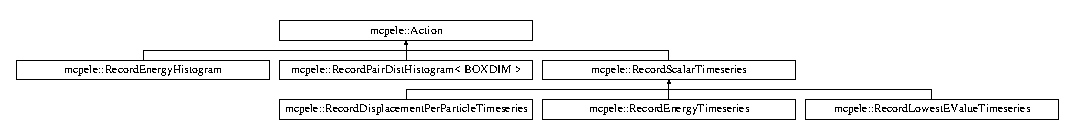
\includegraphics[height=1.377049cm]{classmcpele_1_1Action}
\end{center}
\end{figure}
\subsection*{\-Public \-Member \-Functions}
\begin{DoxyCompactItemize}
\item 
virtual \hyperlink{classmcpele_1_1Action_adee26930d409e327d88b8539b5bb3a67}{$\sim$\-Action} ()
\item 
virtual void \hyperlink{classmcpele_1_1Action_a9500d60c55f0d36ffb6ed0464ea3c68e}{action} (pele\-::\-Array$<$ double $>$ \&coords, double energy, bool accepted, \hyperlink{classmcpele_1_1MC}{\-M\-C} $\ast$mc)=0
\end{DoxyCompactItemize}


\subsection{\-Detailed \-Description}


\-Definition at line 20 of file mc.\-h.



\subsection{\-Constructor \& \-Destructor \-Documentation}
\hypertarget{classmcpele_1_1Action_adee26930d409e327d88b8539b5bb3a67}{\index{mcpele\-::\-Action@{mcpele\-::\-Action}!$\sim$\-Action@{$\sim$\-Action}}
\index{$\sim$\-Action@{$\sim$\-Action}!mcpele::Action@{mcpele\-::\-Action}}
\subsubsection[{$\sim$\-Action}]{\setlength{\rightskip}{0pt plus 5cm}virtual {\bf mcpele\-::\-Action\-::$\sim$\-Action} (
\begin{DoxyParamCaption}
{}
\end{DoxyParamCaption}
)\hspace{0.3cm}{\ttfamily  \mbox{[}inline, virtual\mbox{]}}}}\label{classmcpele_1_1Action_adee26930d409e327d88b8539b5bb3a67}


\-Definition at line 24 of file mc.\-h.



\subsection{\-Member \-Function \-Documentation}
\hypertarget{classmcpele_1_1Action_a9500d60c55f0d36ffb6ed0464ea3c68e}{\index{mcpele\-::\-Action@{mcpele\-::\-Action}!action@{action}}
\index{action@{action}!mcpele::Action@{mcpele\-::\-Action}}
\subsubsection[{action}]{\setlength{\rightskip}{0pt plus 5cm}virtual void {\bf mcpele\-::\-Action\-::action} (
\begin{DoxyParamCaption}
\item[{pele\-::\-Array$<$ double $>$ \&}]{coords, }
\item[{double}]{energy, }
\item[{bool}]{accepted, }
\item[{{\bf \-M\-C} $\ast$}]{mc}
\end{DoxyParamCaption}
)\hspace{0.3cm}{\ttfamily  \mbox{[}pure virtual\mbox{]}}}}\label{classmcpele_1_1Action_a9500d60c55f0d36ffb6ed0464ea3c68e}


\-Implemented in \hyperlink{classmcpele_1_1RecordPairDistHistogram_a2b0d3af344db398ce16e0a473f7f55c4}{mcpele\-::\-Record\-Pair\-Dist\-Histogram$<$ B\-O\-X\-D\-I\-M $>$}, \hyperlink{classmcpele_1_1RecordEnergyHistogram_af0aa711e4556dff5ae5837e42be17ecc}{mcpele\-::\-Record\-Energy\-Histogram}, and \hyperlink{classmcpele_1_1RecordScalarTimeseries_a7cc733d8f0b8daebf4da92423793b9c7}{mcpele\-::\-Record\-Scalar\-Timeseries}.



\-The documentation for this class was generated from the following file\-:\begin{DoxyCompactItemize}
\item 
mcpele/\hyperlink{mc_8h}{mc.\-h}\end{DoxyCompactItemize}

\hypertarget{classmcpele_1_1AdaptiveTakeStep}{\section{mcpele\-:\-:\-Adaptive\-Take\-Step \-Class \-Reference}
\label{classmcpele_1_1AdaptiveTakeStep}\index{mcpele\-::\-Adaptive\-Take\-Step@{mcpele\-::\-Adaptive\-Take\-Step}}
}


{\ttfamily \#include $<$adaptive\-\_\-takestep.\-h$>$}

\-Inheritance diagram for mcpele\-:\-:\-Adaptive\-Take\-Step\-:\begin{figure}[H]
\begin{center}
\leavevmode
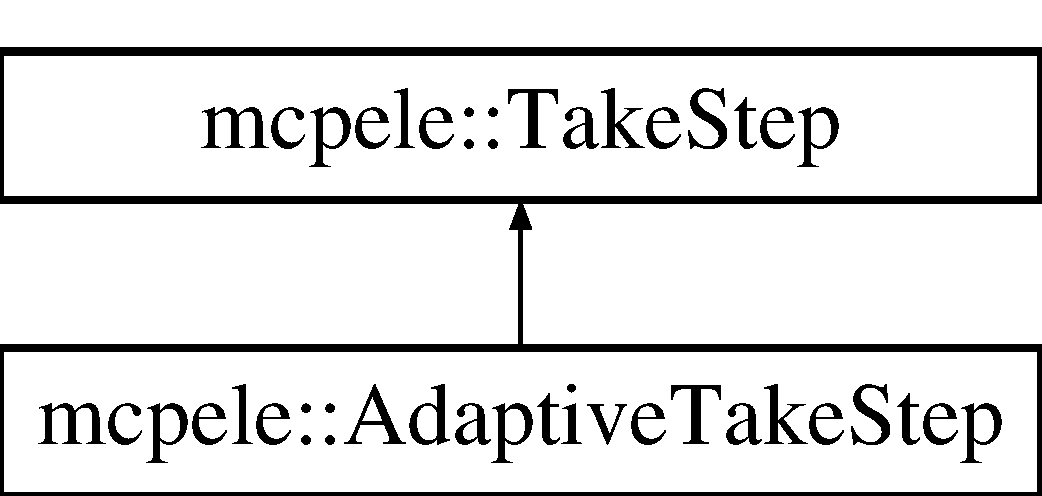
\includegraphics[height=2.000000cm]{classmcpele_1_1AdaptiveTakeStep}
\end{center}
\end{figure}
\subsection*{\-Public \-Member \-Functions}
\begin{DoxyCompactItemize}
\item 
virtual \hyperlink{classmcpele_1_1AdaptiveTakeStep_a6f42dbb0ed0d9dcd88b47e267368b34f}{$\sim$\-Adaptive\-Take\-Step} ()
\item 
\hyperlink{classmcpele_1_1AdaptiveTakeStep_a1ee619caed0973ddea12e0d1a4ce8e9d}{\-Adaptive\-Take\-Step} (std\-::shared\-\_\-ptr$<$ \hyperlink{classmcpele_1_1TakeStep}{\-Take\-Step} $>$ ts, const size\-\_\-t interval=100, const double factor=0.\-9, const double min\-\_\-acceptance\-\_\-ratio=0.\-2, const double max\-\_\-acceptance\-\_\-ratio=0.\-5)
\item 
void \hyperlink{classmcpele_1_1AdaptiveTakeStep_a63b75b0fda5b685fdfd8076f1e099523}{displace} (pele\-::\-Array$<$ double $>$ \&coords, \hyperlink{classmcpele_1_1MC}{\-M\-C} $\ast$mc)
\item 
void \hyperlink{classmcpele_1_1AdaptiveTakeStep_a3787085dd0bdf41fee0787c13265edea}{report} (pele\-::\-Array$<$ double $>$ \&old\-\_\-coords, const double old\-\_\-energy, pele\-::\-Array$<$ double $>$ \&new\-\_\-coords, const double new\-\_\-energy, const bool success, \hyperlink{classmcpele_1_1MC}{\-M\-C} $\ast$mc)
\item 
double \hyperlink{classmcpele_1_1AdaptiveTakeStep_ac3693c26dbad6a3a1f5003626da0eff4}{get\-\_\-min\-\_\-acceptance\-\_\-ratio} () const 
\item 
double \hyperlink{classmcpele_1_1AdaptiveTakeStep_a245d6ab24dce23791a2a75fd896b21e5}{get\-\_\-max\-\_\-acceptance\-\_\-ratio} () const 
\end{DoxyCompactItemize}
\subsection*{\-Protected \-Attributes}
\begin{DoxyCompactItemize}
\item 
std\-::shared\-\_\-ptr$<$ \hyperlink{classmcpele_1_1TakeStep}{\-Take\-Step} $>$ \hyperlink{classmcpele_1_1AdaptiveTakeStep_a2f43525fa8608daabab615459b3ae42a}{m\-\_\-ts}
\item 
size\-\_\-t \hyperlink{classmcpele_1_1AdaptiveTakeStep_ac16baa470b559d1c994be4cebc331b90}{m\-\_\-interval}
\item 
size\-\_\-t \hyperlink{classmcpele_1_1AdaptiveTakeStep_a40288a04fe0de43963d7e6284b1a44e3}{m\-\_\-total\-\_\-steps}
\item 
size\-\_\-t \hyperlink{classmcpele_1_1AdaptiveTakeStep_a5702f4198611fc3b2fa31d7dc27ba1b4}{m\-\_\-accepted\-\_\-steps}
\item 
const double \hyperlink{classmcpele_1_1AdaptiveTakeStep_a82892e788ff27d943cb3845210fb9229}{m\-\_\-factor}
\item 
const double \hyperlink{classmcpele_1_1AdaptiveTakeStep_ad6c2c748b3effbbb8ab2cec826419e88}{m\-\_\-min\-\_\-acceptance\-\_\-ratio}
\item 
const double \hyperlink{classmcpele_1_1AdaptiveTakeStep_a2f83a3b74b5a6d515687e5c02292f9c9}{m\-\_\-max\-\_\-acceptance\-\_\-ratio}
\end{DoxyCompactItemize}


\subsection{\-Detailed \-Description}


\-Definition at line 8 of file adaptive\-\_\-takestep.\-h.



\subsection{\-Constructor \& \-Destructor \-Documentation}
\hypertarget{classmcpele_1_1AdaptiveTakeStep_a6f42dbb0ed0d9dcd88b47e267368b34f}{\index{mcpele\-::\-Adaptive\-Take\-Step@{mcpele\-::\-Adaptive\-Take\-Step}!$\sim$\-Adaptive\-Take\-Step@{$\sim$\-Adaptive\-Take\-Step}}
\index{$\sim$\-Adaptive\-Take\-Step@{$\sim$\-Adaptive\-Take\-Step}!mcpele::AdaptiveTakeStep@{mcpele\-::\-Adaptive\-Take\-Step}}
\subsubsection[{$\sim$\-Adaptive\-Take\-Step}]{\setlength{\rightskip}{0pt plus 5cm}virtual {\bf mcpele\-::\-Adaptive\-Take\-Step\-::$\sim$\-Adaptive\-Take\-Step} (
\begin{DoxyParamCaption}
{}
\end{DoxyParamCaption}
)\hspace{0.3cm}{\ttfamily  \mbox{[}inline, virtual\mbox{]}}}}\label{classmcpele_1_1AdaptiveTakeStep_a6f42dbb0ed0d9dcd88b47e267368b34f}


\-Definition at line 18 of file adaptive\-\_\-takestep.\-h.

\hypertarget{classmcpele_1_1AdaptiveTakeStep_a1ee619caed0973ddea12e0d1a4ce8e9d}{\index{mcpele\-::\-Adaptive\-Take\-Step@{mcpele\-::\-Adaptive\-Take\-Step}!\-Adaptive\-Take\-Step@{\-Adaptive\-Take\-Step}}
\index{\-Adaptive\-Take\-Step@{\-Adaptive\-Take\-Step}!mcpele::AdaptiveTakeStep@{mcpele\-::\-Adaptive\-Take\-Step}}
\subsubsection[{\-Adaptive\-Take\-Step}]{\setlength{\rightskip}{0pt plus 5cm}{\bf mcpele\-::\-Adaptive\-Take\-Step\-::\-Adaptive\-Take\-Step} (
\begin{DoxyParamCaption}
\item[{std\-::shared\-\_\-ptr$<$ {\bf \-Take\-Step} $>$}]{ts, }
\item[{const size\-\_\-t}]{interval = {\ttfamily 100}, }
\item[{const double}]{factor = {\ttfamily 0.9}, }
\item[{const double}]{min\-\_\-acceptance\-\_\-ratio = {\ttfamily 0.2}, }
\item[{const double}]{max\-\_\-acceptance\-\_\-ratio = {\ttfamily 0.5}}
\end{DoxyParamCaption}
)}}\label{classmcpele_1_1AdaptiveTakeStep_a1ee619caed0973ddea12e0d1a4ce8e9d}


\-Definition at line 5 of file adaptive\-\_\-takestep.\-cpp.



\subsection{\-Member \-Function \-Documentation}
\hypertarget{classmcpele_1_1AdaptiveTakeStep_a63b75b0fda5b685fdfd8076f1e099523}{\index{mcpele\-::\-Adaptive\-Take\-Step@{mcpele\-::\-Adaptive\-Take\-Step}!displace@{displace}}
\index{displace@{displace}!mcpele::AdaptiveTakeStep@{mcpele\-::\-Adaptive\-Take\-Step}}
\subsubsection[{displace}]{\setlength{\rightskip}{0pt plus 5cm}void {\bf mcpele\-::\-Adaptive\-Take\-Step\-::displace} (
\begin{DoxyParamCaption}
\item[{pele\-::\-Array$<$ double $>$ \&}]{coords, }
\item[{{\bf \-M\-C} $\ast$}]{mc}
\end{DoxyParamCaption}
)\hspace{0.3cm}{\ttfamily  \mbox{[}inline, virtual\mbox{]}}}}\label{classmcpele_1_1AdaptiveTakeStep_a63b75b0fda5b685fdfd8076f1e099523}


\-Implements \hyperlink{classmcpele_1_1TakeStep_ac3032e0d99d4aa5f940ffea4a28442f5}{mcpele\-::\-Take\-Step}.



\-Definition at line 22 of file adaptive\-\_\-takestep.\-h.

\hypertarget{classmcpele_1_1AdaptiveTakeStep_a245d6ab24dce23791a2a75fd896b21e5}{\index{mcpele\-::\-Adaptive\-Take\-Step@{mcpele\-::\-Adaptive\-Take\-Step}!get\-\_\-max\-\_\-acceptance\-\_\-ratio@{get\-\_\-max\-\_\-acceptance\-\_\-ratio}}
\index{get\-\_\-max\-\_\-acceptance\-\_\-ratio@{get\-\_\-max\-\_\-acceptance\-\_\-ratio}!mcpele::AdaptiveTakeStep@{mcpele\-::\-Adaptive\-Take\-Step}}
\subsubsection[{get\-\_\-max\-\_\-acceptance\-\_\-ratio}]{\setlength{\rightskip}{0pt plus 5cm}double {\bf mcpele\-::\-Adaptive\-Take\-Step\-::get\-\_\-max\-\_\-acceptance\-\_\-ratio} (
\begin{DoxyParamCaption}
{}
\end{DoxyParamCaption}
) const\hspace{0.3cm}{\ttfamily  \mbox{[}inline\mbox{]}}}}\label{classmcpele_1_1AdaptiveTakeStep_a245d6ab24dce23791a2a75fd896b21e5}


\-Definition at line 27 of file adaptive\-\_\-takestep.\-h.

\hypertarget{classmcpele_1_1AdaptiveTakeStep_ac3693c26dbad6a3a1f5003626da0eff4}{\index{mcpele\-::\-Adaptive\-Take\-Step@{mcpele\-::\-Adaptive\-Take\-Step}!get\-\_\-min\-\_\-acceptance\-\_\-ratio@{get\-\_\-min\-\_\-acceptance\-\_\-ratio}}
\index{get\-\_\-min\-\_\-acceptance\-\_\-ratio@{get\-\_\-min\-\_\-acceptance\-\_\-ratio}!mcpele::AdaptiveTakeStep@{mcpele\-::\-Adaptive\-Take\-Step}}
\subsubsection[{get\-\_\-min\-\_\-acceptance\-\_\-ratio}]{\setlength{\rightskip}{0pt plus 5cm}double {\bf mcpele\-::\-Adaptive\-Take\-Step\-::get\-\_\-min\-\_\-acceptance\-\_\-ratio} (
\begin{DoxyParamCaption}
{}
\end{DoxyParamCaption}
) const\hspace{0.3cm}{\ttfamily  \mbox{[}inline\mbox{]}}}}\label{classmcpele_1_1AdaptiveTakeStep_ac3693c26dbad6a3a1f5003626da0eff4}


\-Definition at line 26 of file adaptive\-\_\-takestep.\-h.

\hypertarget{classmcpele_1_1AdaptiveTakeStep_a3787085dd0bdf41fee0787c13265edea}{\index{mcpele\-::\-Adaptive\-Take\-Step@{mcpele\-::\-Adaptive\-Take\-Step}!report@{report}}
\index{report@{report}!mcpele::AdaptiveTakeStep@{mcpele\-::\-Adaptive\-Take\-Step}}
\subsubsection[{report}]{\setlength{\rightskip}{0pt plus 5cm}void {\bf mcpele\-::\-Adaptive\-Take\-Step\-::report} (
\begin{DoxyParamCaption}
\item[{pele\-::\-Array$<$ double $>$ \&}]{old\-\_\-coords, }
\item[{const double}]{old\-\_\-energy, }
\item[{pele\-::\-Array$<$ double $>$ \&}]{new\-\_\-coords, }
\item[{const double}]{new\-\_\-energy, }
\item[{const bool}]{success, }
\item[{{\bf \-M\-C} $\ast$}]{mc}
\end{DoxyParamCaption}
)\hspace{0.3cm}{\ttfamily  \mbox{[}virtual\mbox{]}}}}\label{classmcpele_1_1AdaptiveTakeStep_a3787085dd0bdf41fee0787c13265edea}


\-Reimplemented from \hyperlink{classmcpele_1_1TakeStep_aac4f30de62c4cbc4d9d31c7629742f64}{mcpele\-::\-Take\-Step}.



\-Definition at line 21 of file adaptive\-\_\-takestep.\-cpp.



\subsection{\-Member \-Data \-Documentation}
\hypertarget{classmcpele_1_1AdaptiveTakeStep_a5702f4198611fc3b2fa31d7dc27ba1b4}{\index{mcpele\-::\-Adaptive\-Take\-Step@{mcpele\-::\-Adaptive\-Take\-Step}!m\-\_\-accepted\-\_\-steps@{m\-\_\-accepted\-\_\-steps}}
\index{m\-\_\-accepted\-\_\-steps@{m\-\_\-accepted\-\_\-steps}!mcpele::AdaptiveTakeStep@{mcpele\-::\-Adaptive\-Take\-Step}}
\subsubsection[{m\-\_\-accepted\-\_\-steps}]{\setlength{\rightskip}{0pt plus 5cm}size\-\_\-t {\bf mcpele\-::\-Adaptive\-Take\-Step\-::m\-\_\-accepted\-\_\-steps}\hspace{0.3cm}{\ttfamily  \mbox{[}protected\mbox{]}}}}\label{classmcpele_1_1AdaptiveTakeStep_a5702f4198611fc3b2fa31d7dc27ba1b4}


\-Definition at line 13 of file adaptive\-\_\-takestep.\-h.

\hypertarget{classmcpele_1_1AdaptiveTakeStep_a82892e788ff27d943cb3845210fb9229}{\index{mcpele\-::\-Adaptive\-Take\-Step@{mcpele\-::\-Adaptive\-Take\-Step}!m\-\_\-factor@{m\-\_\-factor}}
\index{m\-\_\-factor@{m\-\_\-factor}!mcpele::AdaptiveTakeStep@{mcpele\-::\-Adaptive\-Take\-Step}}
\subsubsection[{m\-\_\-factor}]{\setlength{\rightskip}{0pt plus 5cm}const double {\bf mcpele\-::\-Adaptive\-Take\-Step\-::m\-\_\-factor}\hspace{0.3cm}{\ttfamily  \mbox{[}protected\mbox{]}}}}\label{classmcpele_1_1AdaptiveTakeStep_a82892e788ff27d943cb3845210fb9229}


\-Definition at line 14 of file adaptive\-\_\-takestep.\-h.

\hypertarget{classmcpele_1_1AdaptiveTakeStep_ac16baa470b559d1c994be4cebc331b90}{\index{mcpele\-::\-Adaptive\-Take\-Step@{mcpele\-::\-Adaptive\-Take\-Step}!m\-\_\-interval@{m\-\_\-interval}}
\index{m\-\_\-interval@{m\-\_\-interval}!mcpele::AdaptiveTakeStep@{mcpele\-::\-Adaptive\-Take\-Step}}
\subsubsection[{m\-\_\-interval}]{\setlength{\rightskip}{0pt plus 5cm}size\-\_\-t {\bf mcpele\-::\-Adaptive\-Take\-Step\-::m\-\_\-interval}\hspace{0.3cm}{\ttfamily  \mbox{[}protected\mbox{]}}}}\label{classmcpele_1_1AdaptiveTakeStep_ac16baa470b559d1c994be4cebc331b90}


\-Definition at line 11 of file adaptive\-\_\-takestep.\-h.

\hypertarget{classmcpele_1_1AdaptiveTakeStep_a2f83a3b74b5a6d515687e5c02292f9c9}{\index{mcpele\-::\-Adaptive\-Take\-Step@{mcpele\-::\-Adaptive\-Take\-Step}!m\-\_\-max\-\_\-acceptance\-\_\-ratio@{m\-\_\-max\-\_\-acceptance\-\_\-ratio}}
\index{m\-\_\-max\-\_\-acceptance\-\_\-ratio@{m\-\_\-max\-\_\-acceptance\-\_\-ratio}!mcpele::AdaptiveTakeStep@{mcpele\-::\-Adaptive\-Take\-Step}}
\subsubsection[{m\-\_\-max\-\_\-acceptance\-\_\-ratio}]{\setlength{\rightskip}{0pt plus 5cm}const double {\bf mcpele\-::\-Adaptive\-Take\-Step\-::m\-\_\-max\-\_\-acceptance\-\_\-ratio}\hspace{0.3cm}{\ttfamily  \mbox{[}protected\mbox{]}}}}\label{classmcpele_1_1AdaptiveTakeStep_a2f83a3b74b5a6d515687e5c02292f9c9}


\-Definition at line 16 of file adaptive\-\_\-takestep.\-h.

\hypertarget{classmcpele_1_1AdaptiveTakeStep_ad6c2c748b3effbbb8ab2cec826419e88}{\index{mcpele\-::\-Adaptive\-Take\-Step@{mcpele\-::\-Adaptive\-Take\-Step}!m\-\_\-min\-\_\-acceptance\-\_\-ratio@{m\-\_\-min\-\_\-acceptance\-\_\-ratio}}
\index{m\-\_\-min\-\_\-acceptance\-\_\-ratio@{m\-\_\-min\-\_\-acceptance\-\_\-ratio}!mcpele::AdaptiveTakeStep@{mcpele\-::\-Adaptive\-Take\-Step}}
\subsubsection[{m\-\_\-min\-\_\-acceptance\-\_\-ratio}]{\setlength{\rightskip}{0pt plus 5cm}const double {\bf mcpele\-::\-Adaptive\-Take\-Step\-::m\-\_\-min\-\_\-acceptance\-\_\-ratio}\hspace{0.3cm}{\ttfamily  \mbox{[}protected\mbox{]}}}}\label{classmcpele_1_1AdaptiveTakeStep_ad6c2c748b3effbbb8ab2cec826419e88}


\-Definition at line 15 of file adaptive\-\_\-takestep.\-h.

\hypertarget{classmcpele_1_1AdaptiveTakeStep_a40288a04fe0de43963d7e6284b1a44e3}{\index{mcpele\-::\-Adaptive\-Take\-Step@{mcpele\-::\-Adaptive\-Take\-Step}!m\-\_\-total\-\_\-steps@{m\-\_\-total\-\_\-steps}}
\index{m\-\_\-total\-\_\-steps@{m\-\_\-total\-\_\-steps}!mcpele::AdaptiveTakeStep@{mcpele\-::\-Adaptive\-Take\-Step}}
\subsubsection[{m\-\_\-total\-\_\-steps}]{\setlength{\rightskip}{0pt plus 5cm}size\-\_\-t {\bf mcpele\-::\-Adaptive\-Take\-Step\-::m\-\_\-total\-\_\-steps}\hspace{0.3cm}{\ttfamily  \mbox{[}protected\mbox{]}}}}\label{classmcpele_1_1AdaptiveTakeStep_a40288a04fe0de43963d7e6284b1a44e3}


\-Definition at line 12 of file adaptive\-\_\-takestep.\-h.

\hypertarget{classmcpele_1_1AdaptiveTakeStep_a2f43525fa8608daabab615459b3ae42a}{\index{mcpele\-::\-Adaptive\-Take\-Step@{mcpele\-::\-Adaptive\-Take\-Step}!m\-\_\-ts@{m\-\_\-ts}}
\index{m\-\_\-ts@{m\-\_\-ts}!mcpele::AdaptiveTakeStep@{mcpele\-::\-Adaptive\-Take\-Step}}
\subsubsection[{m\-\_\-ts}]{\setlength{\rightskip}{0pt plus 5cm}std\-::shared\-\_\-ptr$<${\bf \-Take\-Step}$>$ {\bf mcpele\-::\-Adaptive\-Take\-Step\-::m\-\_\-ts}\hspace{0.3cm}{\ttfamily  \mbox{[}protected\mbox{]}}}}\label{classmcpele_1_1AdaptiveTakeStep_a2f43525fa8608daabab615459b3ae42a}


\-Definition at line 10 of file adaptive\-\_\-takestep.\-h.



\-The documentation for this class was generated from the following files\-:\begin{DoxyCompactItemize}
\item 
mcpele/\hyperlink{adaptive__takestep_8h}{adaptive\-\_\-takestep.\-h}\item 
\hyperlink{adaptive__takestep_8cpp}{adaptive\-\_\-takestep.\-cpp}\end{DoxyCompactItemize}

\hypertarget{classmcpele_1_1CheckSphericalContainer}{\section{mcpele\-:\-:\-Check\-Spherical\-Container \-Class \-Reference}
\label{classmcpele_1_1CheckSphericalContainer}\index{mcpele\-::\-Check\-Spherical\-Container@{mcpele\-::\-Check\-Spherical\-Container}}
}


{\ttfamily \#include $<$check\-\_\-spherical\-\_\-container.\-h$>$}

\-Inheritance diagram for mcpele\-:\-:\-Check\-Spherical\-Container\-:\begin{figure}[H]
\begin{center}
\leavevmode
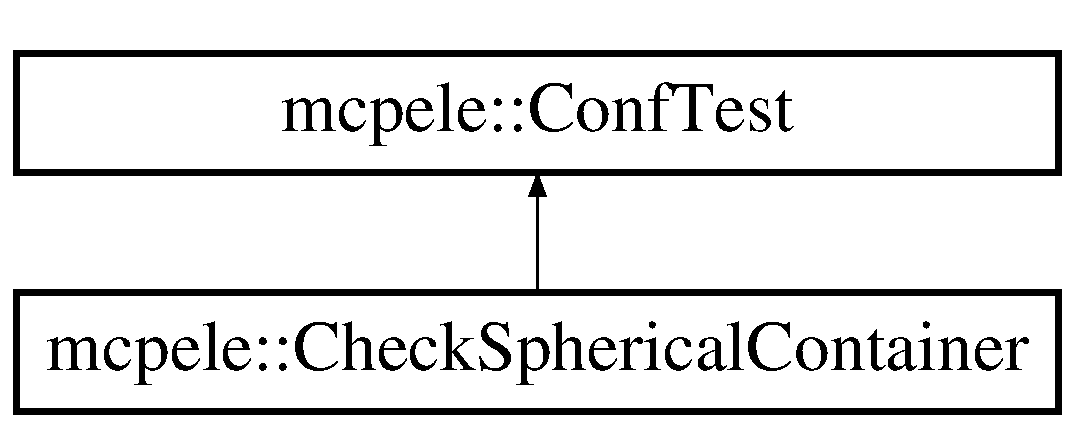
\includegraphics[height=2.000000cm]{classmcpele_1_1CheckSphericalContainer}
\end{center}
\end{figure}
\subsection*{\-Public \-Member \-Functions}
\begin{DoxyCompactItemize}
\item 
\hyperlink{classmcpele_1_1CheckSphericalContainer_af1ddbdb3d2651a18df37447af8749853}{\-Check\-Spherical\-Container} (const double radius, const size\-\_\-t ndim)
\item 
virtual bool \hyperlink{classmcpele_1_1CheckSphericalContainer_a69f1b9e554a00d539477443dedbb3426}{conf\-\_\-test} (pele\-::\-Array$<$ double $>$ \&trial\-\_\-coords, \hyperlink{classmcpele_1_1MC}{\-M\-C} $\ast$mc)
\item 
virtual \hyperlink{classmcpele_1_1CheckSphericalContainer_ae0031a4990e7465c8f550f7bfe367042}{$\sim$\-Check\-Spherical\-Container} ()
\end{DoxyCompactItemize}
\subsection*{\-Protected \-Attributes}
\begin{DoxyCompactItemize}
\item 
double \hyperlink{classmcpele_1_1CheckSphericalContainer_a692b8da3daa2d45a7fc651d2ce045763}{m\-\_\-radius2}
\item 
size\-\_\-t \hyperlink{classmcpele_1_1CheckSphericalContainer_a4c900129e7fe133b1ddd3f9957eb1154}{m\-\_\-ndim}
\end{DoxyCompactItemize}


\subsection{\-Detailed \-Description}


\-Definition at line 18 of file check\-\_\-spherical\-\_\-container.\-h.



\subsection{\-Constructor \& \-Destructor \-Documentation}
\hypertarget{classmcpele_1_1CheckSphericalContainer_af1ddbdb3d2651a18df37447af8749853}{\index{mcpele\-::\-Check\-Spherical\-Container@{mcpele\-::\-Check\-Spherical\-Container}!\-Check\-Spherical\-Container@{\-Check\-Spherical\-Container}}
\index{\-Check\-Spherical\-Container@{\-Check\-Spherical\-Container}!mcpele::CheckSphericalContainer@{mcpele\-::\-Check\-Spherical\-Container}}
\subsubsection[{\-Check\-Spherical\-Container}]{\setlength{\rightskip}{0pt plus 5cm}{\bf mcpele\-::\-Check\-Spherical\-Container\-::\-Check\-Spherical\-Container} (
\begin{DoxyParamCaption}
\item[{const double}]{radius, }
\item[{const size\-\_\-t}]{ndim}
\end{DoxyParamCaption}
)}}\label{classmcpele_1_1CheckSphericalContainer_af1ddbdb3d2651a18df37447af8749853}


\-Definition at line 8 of file check\-\_\-spherical\-\_\-container.\-cpp.

\hypertarget{classmcpele_1_1CheckSphericalContainer_ae0031a4990e7465c8f550f7bfe367042}{\index{mcpele\-::\-Check\-Spherical\-Container@{mcpele\-::\-Check\-Spherical\-Container}!$\sim$\-Check\-Spherical\-Container@{$\sim$\-Check\-Spherical\-Container}}
\index{$\sim$\-Check\-Spherical\-Container@{$\sim$\-Check\-Spherical\-Container}!mcpele::CheckSphericalContainer@{mcpele\-::\-Check\-Spherical\-Container}}
\subsubsection[{$\sim$\-Check\-Spherical\-Container}]{\setlength{\rightskip}{0pt plus 5cm}virtual {\bf mcpele\-::\-Check\-Spherical\-Container\-::$\sim$\-Check\-Spherical\-Container} (
\begin{DoxyParamCaption}
{}
\end{DoxyParamCaption}
)\hspace{0.3cm}{\ttfamily  \mbox{[}inline, virtual\mbox{]}}}}\label{classmcpele_1_1CheckSphericalContainer_ae0031a4990e7465c8f550f7bfe367042}


\-Definition at line 25 of file check\-\_\-spherical\-\_\-container.\-h.



\subsection{\-Member \-Function \-Documentation}
\hypertarget{classmcpele_1_1CheckSphericalContainer_a69f1b9e554a00d539477443dedbb3426}{\index{mcpele\-::\-Check\-Spherical\-Container@{mcpele\-::\-Check\-Spherical\-Container}!conf\-\_\-test@{conf\-\_\-test}}
\index{conf\-\_\-test@{conf\-\_\-test}!mcpele::CheckSphericalContainer@{mcpele\-::\-Check\-Spherical\-Container}}
\subsubsection[{conf\-\_\-test}]{\setlength{\rightskip}{0pt plus 5cm}bool {\bf mcpele\-::\-Check\-Spherical\-Container\-::conf\-\_\-test} (
\begin{DoxyParamCaption}
\item[{pele\-::\-Array$<$ double $>$ \&}]{trial\-\_\-coords, }
\item[{{\bf \-M\-C} $\ast$}]{mc}
\end{DoxyParamCaption}
)\hspace{0.3cm}{\ttfamily  \mbox{[}virtual\mbox{]}}}}\label{classmcpele_1_1CheckSphericalContainer_a69f1b9e554a00d539477443dedbb3426}


\-Implements \hyperlink{classmcpele_1_1ConfTest_ad2757dd936a04849c9657e15a950dd8f}{mcpele\-::\-Conf\-Test}.



\-Definition at line 13 of file check\-\_\-spherical\-\_\-container.\-cpp.



\subsection{\-Member \-Data \-Documentation}
\hypertarget{classmcpele_1_1CheckSphericalContainer_a4c900129e7fe133b1ddd3f9957eb1154}{\index{mcpele\-::\-Check\-Spherical\-Container@{mcpele\-::\-Check\-Spherical\-Container}!m\-\_\-ndim@{m\-\_\-ndim}}
\index{m\-\_\-ndim@{m\-\_\-ndim}!mcpele::CheckSphericalContainer@{mcpele\-::\-Check\-Spherical\-Container}}
\subsubsection[{m\-\_\-ndim}]{\setlength{\rightskip}{0pt plus 5cm}size\-\_\-t {\bf mcpele\-::\-Check\-Spherical\-Container\-::m\-\_\-ndim}\hspace{0.3cm}{\ttfamily  \mbox{[}protected\mbox{]}}}}\label{classmcpele_1_1CheckSphericalContainer_a4c900129e7fe133b1ddd3f9957eb1154}


\-Definition at line 21 of file check\-\_\-spherical\-\_\-container.\-h.

\hypertarget{classmcpele_1_1CheckSphericalContainer_a692b8da3daa2d45a7fc651d2ce045763}{\index{mcpele\-::\-Check\-Spherical\-Container@{mcpele\-::\-Check\-Spherical\-Container}!m\-\_\-radius2@{m\-\_\-radius2}}
\index{m\-\_\-radius2@{m\-\_\-radius2}!mcpele::CheckSphericalContainer@{mcpele\-::\-Check\-Spherical\-Container}}
\subsubsection[{m\-\_\-radius2}]{\setlength{\rightskip}{0pt plus 5cm}double {\bf mcpele\-::\-Check\-Spherical\-Container\-::m\-\_\-radius2}\hspace{0.3cm}{\ttfamily  \mbox{[}protected\mbox{]}}}}\label{classmcpele_1_1CheckSphericalContainer_a692b8da3daa2d45a7fc651d2ce045763}


\-Definition at line 20 of file check\-\_\-spherical\-\_\-container.\-h.



\-The documentation for this class was generated from the following files\-:\begin{DoxyCompactItemize}
\item 
mcpele/\hyperlink{check__spherical__container_8h}{check\-\_\-spherical\-\_\-container.\-h}\item 
\hyperlink{check__spherical__container_8cpp}{check\-\_\-spherical\-\_\-container.\-cpp}\end{DoxyCompactItemize}

\hypertarget{classmcpele_1_1ConfTest}{\section{mcpele\-:\-:\-Conf\-Test \-Class \-Reference}
\label{classmcpele_1_1ConfTest}\index{mcpele\-::\-Conf\-Test@{mcpele\-::\-Conf\-Test}}
}


{\ttfamily \#include $<$mc.\-h$>$}

\-Inheritance diagram for mcpele\-:\-:\-Conf\-Test\-:\begin{figure}[H]
\begin{center}
\leavevmode
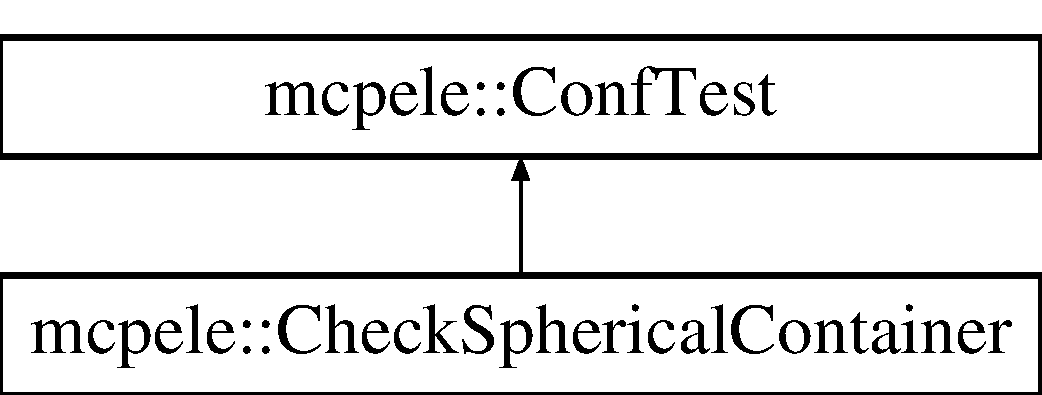
\includegraphics[height=2.000000cm]{classmcpele_1_1ConfTest}
\end{center}
\end{figure}
\subsection*{\-Public \-Member \-Functions}
\begin{DoxyCompactItemize}
\item 
virtual \hyperlink{classmcpele_1_1ConfTest_a8d5a5ff5d0222a2d55e3e6c413559d2a}{$\sim$\-Conf\-Test} ()
\item 
virtual bool \hyperlink{classmcpele_1_1ConfTest_ad2757dd936a04849c9657e15a950dd8f}{conf\-\_\-test} (pele\-::\-Array$<$ double $>$ \&trial\-\_\-coords, \hyperlink{classmcpele_1_1MC}{\-M\-C} $\ast$mc)=0
\end{DoxyCompactItemize}


\subsection{\-Detailed \-Description}


\-Definition at line 47 of file mc.\-h.



\subsection{\-Constructor \& \-Destructor \-Documentation}
\hypertarget{classmcpele_1_1ConfTest_a8d5a5ff5d0222a2d55e3e6c413559d2a}{\index{mcpele\-::\-Conf\-Test@{mcpele\-::\-Conf\-Test}!$\sim$\-Conf\-Test@{$\sim$\-Conf\-Test}}
\index{$\sim$\-Conf\-Test@{$\sim$\-Conf\-Test}!mcpele::ConfTest@{mcpele\-::\-Conf\-Test}}
\subsubsection[{$\sim$\-Conf\-Test}]{\setlength{\rightskip}{0pt plus 5cm}virtual {\bf mcpele\-::\-Conf\-Test\-::$\sim$\-Conf\-Test} (
\begin{DoxyParamCaption}
{}
\end{DoxyParamCaption}
)\hspace{0.3cm}{\ttfamily  \mbox{[}inline, virtual\mbox{]}}}}\label{classmcpele_1_1ConfTest_a8d5a5ff5d0222a2d55e3e6c413559d2a}


\-Definition at line 51 of file mc.\-h.



\subsection{\-Member \-Function \-Documentation}
\hypertarget{classmcpele_1_1ConfTest_ad2757dd936a04849c9657e15a950dd8f}{\index{mcpele\-::\-Conf\-Test@{mcpele\-::\-Conf\-Test}!conf\-\_\-test@{conf\-\_\-test}}
\index{conf\-\_\-test@{conf\-\_\-test}!mcpele::ConfTest@{mcpele\-::\-Conf\-Test}}
\subsubsection[{conf\-\_\-test}]{\setlength{\rightskip}{0pt plus 5cm}virtual bool {\bf mcpele\-::\-Conf\-Test\-::conf\-\_\-test} (
\begin{DoxyParamCaption}
\item[{pele\-::\-Array$<$ double $>$ \&}]{trial\-\_\-coords, }
\item[{{\bf \-M\-C} $\ast$}]{mc}
\end{DoxyParamCaption}
)\hspace{0.3cm}{\ttfamily  \mbox{[}pure virtual\mbox{]}}}}\label{classmcpele_1_1ConfTest_ad2757dd936a04849c9657e15a950dd8f}


\-Implemented in \hyperlink{classmcpele_1_1CheckSphericalContainer_a69f1b9e554a00d539477443dedbb3426}{mcpele\-::\-Check\-Spherical\-Container}.



\-The documentation for this class was generated from the following file\-:\begin{DoxyCompactItemize}
\item 
mcpele/\hyperlink{mc_8h}{mc.\-h}\end{DoxyCompactItemize}

\hypertarget{classmcpele_1_1EnergyWindowTest}{\section{mcpele\-:\-:\-Energy\-Window\-Test \-Class \-Reference}
\label{classmcpele_1_1EnergyWindowTest}\index{mcpele\-::\-Energy\-Window\-Test@{mcpele\-::\-Energy\-Window\-Test}}
}


{\ttfamily \#include $<$energy\-\_\-window\-\_\-test.\-h$>$}

\-Inheritance diagram for mcpele\-:\-:\-Energy\-Window\-Test\-:\begin{figure}[H]
\begin{center}
\leavevmode
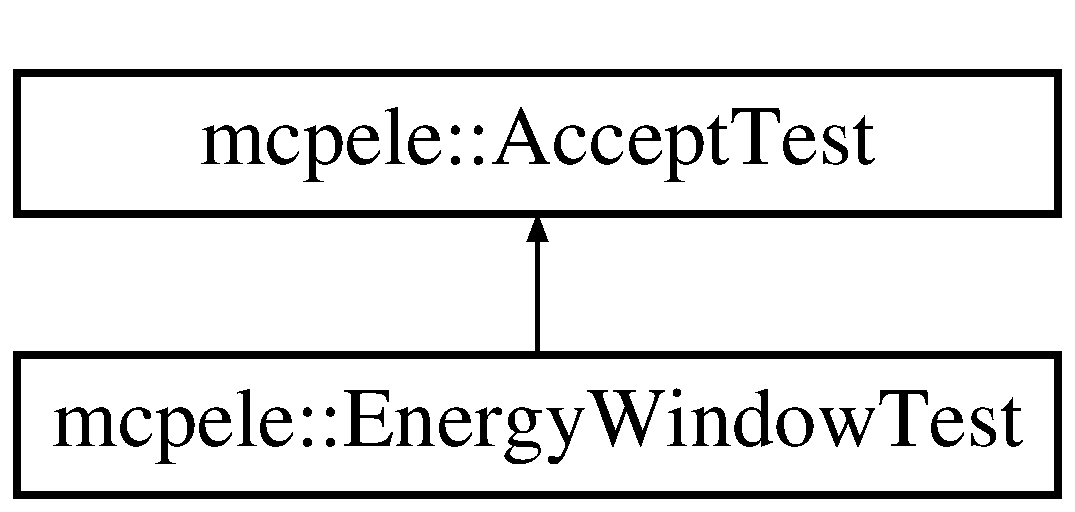
\includegraphics[height=2.000000cm]{classmcpele_1_1EnergyWindowTest}
\end{center}
\end{figure}
\subsection*{\-Public \-Member \-Functions}
\begin{DoxyCompactItemize}
\item 
\hyperlink{classmcpele_1_1EnergyWindowTest_a0b8f02bf14f23525e1661729864d8e70}{\-Energy\-Window\-Test} (const double min\-\_\-energy, const double max\-\_\-energy)
\item 
virtual \hyperlink{classmcpele_1_1EnergyWindowTest_ad0e1111aaf29e6c462451d7708722c52}{$\sim$\-Energy\-Window\-Test} ()
\item 
virtual bool \hyperlink{classmcpele_1_1EnergyWindowTest_a529460eac573357f981639fe85807520}{test} (pele\-::\-Array$<$ double $>$ \&trial\-\_\-coords, double trial\-\_\-energy, pele\-::\-Array$<$ double $>$ \&old\-\_\-coords, double old\-\_\-energy, double temperature, \hyperlink{classmcpele_1_1MC}{\-M\-C} $\ast$mc)
\end{DoxyCompactItemize}
\subsection*{\-Protected \-Attributes}
\begin{DoxyCompactItemize}
\item 
double \hyperlink{classmcpele_1_1EnergyWindowTest_abb86cad9952f92fd8db221baaf62e847}{m\-\_\-min\-\_\-energy}
\item 
double \hyperlink{classmcpele_1_1EnergyWindowTest_ae0db5a8b295b8bf29477fd5dd741a88c}{m\-\_\-max\-\_\-energy}
\end{DoxyCompactItemize}


\subsection{\-Detailed \-Description}
\-Energy window test \-This test checks that the energy of the system stays within a certain energy window 

\-Definition at line 14 of file energy\-\_\-window\-\_\-test.\-h.



\subsection{\-Constructor \& \-Destructor \-Documentation}
\hypertarget{classmcpele_1_1EnergyWindowTest_a0b8f02bf14f23525e1661729864d8e70}{\index{mcpele\-::\-Energy\-Window\-Test@{mcpele\-::\-Energy\-Window\-Test}!\-Energy\-Window\-Test@{\-Energy\-Window\-Test}}
\index{\-Energy\-Window\-Test@{\-Energy\-Window\-Test}!mcpele::EnergyWindowTest@{mcpele\-::\-Energy\-Window\-Test}}
\subsubsection[{\-Energy\-Window\-Test}]{\setlength{\rightskip}{0pt plus 5cm}{\bf mcpele\-::\-Energy\-Window\-Test\-::\-Energy\-Window\-Test} (
\begin{DoxyParamCaption}
\item[{const double}]{min\-\_\-energy, }
\item[{const double}]{max\-\_\-energy}
\end{DoxyParamCaption}
)}}\label{classmcpele_1_1EnergyWindowTest_a0b8f02bf14f23525e1661729864d8e70}


\-Definition at line 9 of file energy\-\_\-window\-\_\-test.\-cpp.

\hypertarget{classmcpele_1_1EnergyWindowTest_ad0e1111aaf29e6c462451d7708722c52}{\index{mcpele\-::\-Energy\-Window\-Test@{mcpele\-::\-Energy\-Window\-Test}!$\sim$\-Energy\-Window\-Test@{$\sim$\-Energy\-Window\-Test}}
\index{$\sim$\-Energy\-Window\-Test@{$\sim$\-Energy\-Window\-Test}!mcpele::EnergyWindowTest@{mcpele\-::\-Energy\-Window\-Test}}
\subsubsection[{$\sim$\-Energy\-Window\-Test}]{\setlength{\rightskip}{0pt plus 5cm}virtual {\bf mcpele\-::\-Energy\-Window\-Test\-::$\sim$\-Energy\-Window\-Test} (
\begin{DoxyParamCaption}
{}
\end{DoxyParamCaption}
)\hspace{0.3cm}{\ttfamily  \mbox{[}inline, virtual\mbox{]}}}}\label{classmcpele_1_1EnergyWindowTest_ad0e1111aaf29e6c462451d7708722c52}


\-Definition at line 20 of file energy\-\_\-window\-\_\-test.\-h.



\subsection{\-Member \-Function \-Documentation}
\hypertarget{classmcpele_1_1EnergyWindowTest_a529460eac573357f981639fe85807520}{\index{mcpele\-::\-Energy\-Window\-Test@{mcpele\-::\-Energy\-Window\-Test}!test@{test}}
\index{test@{test}!mcpele::EnergyWindowTest@{mcpele\-::\-Energy\-Window\-Test}}
\subsubsection[{test}]{\setlength{\rightskip}{0pt plus 5cm}bool {\bf mcpele\-::\-Energy\-Window\-Test\-::test} (
\begin{DoxyParamCaption}
\item[{pele\-::\-Array$<$ double $>$ \&}]{trial\-\_\-coords, }
\item[{double}]{trial\-\_\-energy, }
\item[{pele\-::\-Array$<$ double $>$ \&}]{old\-\_\-coords, }
\item[{double}]{old\-\_\-energy, }
\item[{double}]{temperature, }
\item[{{\bf \-M\-C} $\ast$}]{mc}
\end{DoxyParamCaption}
)\hspace{0.3cm}{\ttfamily  \mbox{[}virtual\mbox{]}}}}\label{classmcpele_1_1EnergyWindowTest_a529460eac573357f981639fe85807520}


\-Implements \hyperlink{classmcpele_1_1AcceptTest_ae2d9e2feaae60d49a35c7170f56f5d78}{mcpele\-::\-Accept\-Test}.



\-Definition at line 14 of file energy\-\_\-window\-\_\-test.\-cpp.



\subsection{\-Member \-Data \-Documentation}
\hypertarget{classmcpele_1_1EnergyWindowTest_ae0db5a8b295b8bf29477fd5dd741a88c}{\index{mcpele\-::\-Energy\-Window\-Test@{mcpele\-::\-Energy\-Window\-Test}!m\-\_\-max\-\_\-energy@{m\-\_\-max\-\_\-energy}}
\index{m\-\_\-max\-\_\-energy@{m\-\_\-max\-\_\-energy}!mcpele::EnergyWindowTest@{mcpele\-::\-Energy\-Window\-Test}}
\subsubsection[{m\-\_\-max\-\_\-energy}]{\setlength{\rightskip}{0pt plus 5cm}double {\bf mcpele\-::\-Energy\-Window\-Test\-::m\-\_\-max\-\_\-energy}\hspace{0.3cm}{\ttfamily  \mbox{[}protected\mbox{]}}}}\label{classmcpele_1_1EnergyWindowTest_ae0db5a8b295b8bf29477fd5dd741a88c}


\-Definition at line 17 of file energy\-\_\-window\-\_\-test.\-h.

\hypertarget{classmcpele_1_1EnergyWindowTest_abb86cad9952f92fd8db221baaf62e847}{\index{mcpele\-::\-Energy\-Window\-Test@{mcpele\-::\-Energy\-Window\-Test}!m\-\_\-min\-\_\-energy@{m\-\_\-min\-\_\-energy}}
\index{m\-\_\-min\-\_\-energy@{m\-\_\-min\-\_\-energy}!mcpele::EnergyWindowTest@{mcpele\-::\-Energy\-Window\-Test}}
\subsubsection[{m\-\_\-min\-\_\-energy}]{\setlength{\rightskip}{0pt plus 5cm}double {\bf mcpele\-::\-Energy\-Window\-Test\-::m\-\_\-min\-\_\-energy}\hspace{0.3cm}{\ttfamily  \mbox{[}protected\mbox{]}}}}\label{classmcpele_1_1EnergyWindowTest_abb86cad9952f92fd8db221baaf62e847}


\-Definition at line 16 of file energy\-\_\-window\-\_\-test.\-h.



\-The documentation for this class was generated from the following files\-:\begin{DoxyCompactItemize}
\item 
mcpele/\hyperlink{energy__window__test_8h}{energy\-\_\-window\-\_\-test.\-h}\item 
\hyperlink{energy__window__test_8cpp}{energy\-\_\-window\-\_\-test.\-cpp}\end{DoxyCompactItemize}

\hypertarget{classmcpele_1_1FindLowestEigenvalue}{\section{mcpele\-:\-:\-Find\-Lowest\-Eigenvalue \-Class \-Reference}
\label{classmcpele_1_1FindLowestEigenvalue}\index{mcpele\-::\-Find\-Lowest\-Eigenvalue@{mcpele\-::\-Find\-Lowest\-Eigenvalue}}
}


{\ttfamily \#include $<$lowest\-\_\-eigenvalue.\-h$>$}

\subsection*{\-Public \-Member \-Functions}
\begin{DoxyCompactItemize}
\item 
\hyperlink{classmcpele_1_1FindLowestEigenvalue_aa8cff93dfc74754b4bd4f290d852a7a0}{\-Find\-Lowest\-Eigenvalue} (std\-::shared\-\_\-ptr$<$ pele\-::\-Base\-Potential $>$ landscape\-\_\-potential, const size\-\_\-t boxdimension, const pele\-::\-Array$<$ double $>$ ranvec, const size\-\_\-t lbfgsniter)
\item 
double \hyperlink{classmcpele_1_1FindLowestEigenvalue_a29f56a74823d7e974187b1a04ff44639}{compute\-\_\-lowest\-\_\-eigenvalue} (pele\-::\-Array$<$ double $>$ coords)
\end{DoxyCompactItemize}


\subsection{\-Detailed \-Description}


\-Definition at line 11 of file lowest\-\_\-eigenvalue.\-h.



\subsection{\-Constructor \& \-Destructor \-Documentation}
\hypertarget{classmcpele_1_1FindLowestEigenvalue_aa8cff93dfc74754b4bd4f290d852a7a0}{\index{mcpele\-::\-Find\-Lowest\-Eigenvalue@{mcpele\-::\-Find\-Lowest\-Eigenvalue}!\-Find\-Lowest\-Eigenvalue@{\-Find\-Lowest\-Eigenvalue}}
\index{\-Find\-Lowest\-Eigenvalue@{\-Find\-Lowest\-Eigenvalue}!mcpele::FindLowestEigenvalue@{mcpele\-::\-Find\-Lowest\-Eigenvalue}}
\subsubsection[{\-Find\-Lowest\-Eigenvalue}]{\setlength{\rightskip}{0pt plus 5cm}{\bf mcpele\-::\-Find\-Lowest\-Eigenvalue\-::\-Find\-Lowest\-Eigenvalue} (
\begin{DoxyParamCaption}
\item[{std\-::shared\-\_\-ptr$<$ pele\-::\-Base\-Potential $>$}]{landscape\-\_\-potential, }
\item[{const size\-\_\-t}]{boxdimension, }
\item[{const pele\-::\-Array$<$ double $>$}]{ranvec, }
\item[{const size\-\_\-t}]{lbfgsniter}
\end{DoxyParamCaption}
)}}\label{classmcpele_1_1FindLowestEigenvalue_aa8cff93dfc74754b4bd4f290d852a7a0}


\-Definition at line 7 of file lowest\-\_\-eigenvalue.\-cpp.



\subsection{\-Member \-Function \-Documentation}
\hypertarget{classmcpele_1_1FindLowestEigenvalue_a29f56a74823d7e974187b1a04ff44639}{\index{mcpele\-::\-Find\-Lowest\-Eigenvalue@{mcpele\-::\-Find\-Lowest\-Eigenvalue}!compute\-\_\-lowest\-\_\-eigenvalue@{compute\-\_\-lowest\-\_\-eigenvalue}}
\index{compute\-\_\-lowest\-\_\-eigenvalue@{compute\-\_\-lowest\-\_\-eigenvalue}!mcpele::FindLowestEigenvalue@{mcpele\-::\-Find\-Lowest\-Eigenvalue}}
\subsubsection[{compute\-\_\-lowest\-\_\-eigenvalue}]{\setlength{\rightskip}{0pt plus 5cm}double {\bf mcpele\-::\-Find\-Lowest\-Eigenvalue\-::compute\-\_\-lowest\-\_\-eigenvalue} (
\begin{DoxyParamCaption}
\item[{pele\-::\-Array$<$ double $>$}]{coords}
\end{DoxyParamCaption}
)}}\label{classmcpele_1_1FindLowestEigenvalue_a29f56a74823d7e974187b1a04ff44639}


\-Definition at line 19 of file lowest\-\_\-eigenvalue.\-cpp.



\-The documentation for this class was generated from the following files\-:\begin{DoxyCompactItemize}
\item 
mcpele/\hyperlink{lowest__eigenvalue_8h}{lowest\-\_\-eigenvalue.\-h}\item 
\hyperlink{lowest__eigenvalue_8cpp}{lowest\-\_\-eigenvalue.\-cpp}\end{DoxyCompactItemize}

\hypertarget{classmcpele_1_1GaussianCoordsDisplacement}{\section{mcpele\-:\-:\-Gaussian\-Coords\-Displacement \-Class \-Reference}
\label{classmcpele_1_1GaussianCoordsDisplacement}\index{mcpele\-::\-Gaussian\-Coords\-Displacement@{mcpele\-::\-Gaussian\-Coords\-Displacement}}
}


{\ttfamily \#include $<$gaussian\-\_\-coords\-\_\-displacement.\-h$>$}

\-Inheritance diagram for mcpele\-:\-:\-Gaussian\-Coords\-Displacement\-:\begin{figure}[H]
\begin{center}
\leavevmode
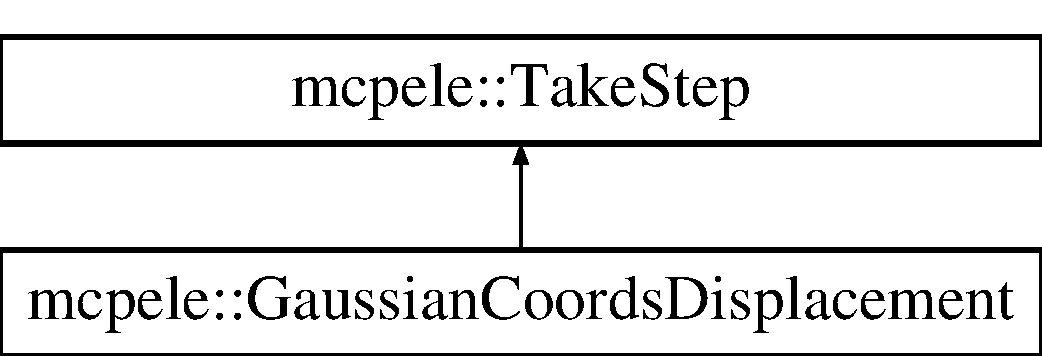
\includegraphics[height=2.000000cm]{classmcpele_1_1GaussianCoordsDisplacement}
\end{center}
\end{figure}
\subsection*{\-Public \-Member \-Functions}
\begin{DoxyCompactItemize}
\item 
\hyperlink{classmcpele_1_1GaussianCoordsDisplacement_a693f5cd3743cca41cfae62ba5c8fa1b2}{\-Gaussian\-Coords\-Displacement} (const size\-\_\-t rseed, const double stepsize)
\item 
virtual \hyperlink{classmcpele_1_1GaussianCoordsDisplacement_a5629b7e1fc63a2208a188a7ed0461acc}{$\sim$\-Gaussian\-Coords\-Displacement} ()
\item 
virtual void \hyperlink{classmcpele_1_1GaussianCoordsDisplacement_a9855e838fb6d19c55be12dd108cfdb5b}{displace} (pele\-::\-Array$<$ double $>$ \&coords, \hyperlink{classmcpele_1_1MC}{\-M\-C} $\ast$mc)
\item 
size\-\_\-t \hyperlink{classmcpele_1_1GaussianCoordsDisplacement_acb65b915f740d1618ecc267c02fcd17b}{get\-\_\-seed} () const 
\item 
void \hyperlink{classmcpele_1_1GaussianCoordsDisplacement_adaefd98609344bb8a9744a9cee554ccc}{set\-\_\-generator\-\_\-seed} (const size\-\_\-t inp)
\item 
double \hyperlink{classmcpele_1_1GaussianCoordsDisplacement_a5f7da29b7bde371ff3971164f58ff3d9}{expected\-\_\-mean} () const 
\item 
double \hyperlink{classmcpele_1_1GaussianCoordsDisplacement_a225423c83abb6d91bedac92802961790}{expected\-\_\-variance} (const double ss) const 
\item 
double \hyperlink{classmcpele_1_1GaussianCoordsDisplacement_a87e64b4fed1cf85cc6e4ee13d6fde190}{get\-\_\-stepsize} () const 
\item 
void \hyperlink{classmcpele_1_1GaussianCoordsDisplacement_ab36a3671f18d4b2560cfc981a6bd6a2d}{set\-\_\-stepsize} (const double input)
\item 
size\-\_\-t \hyperlink{classmcpele_1_1GaussianCoordsDisplacement_ae5042527322a279d5a151ae7879d647e}{get\-\_\-count} () const 
\end{DoxyCompactItemize}
\subsection*{\-Protected \-Attributes}
\begin{DoxyCompactItemize}
\item 
size\-\_\-t \hyperlink{classmcpele_1_1GaussianCoordsDisplacement_af50ffc7add2d8e7ae70b07c04a620fb7}{m\-\_\-seed}
\item 
double \hyperlink{classmcpele_1_1GaussianCoordsDisplacement_a515b27b041db3301e85bd4da6ba44383}{m\-\_\-mean}
\item 
double \hyperlink{classmcpele_1_1GaussianCoordsDisplacement_a49258ed3098c51b3567e7193ccd57e70}{m\-\_\-stdev}
\item 
std\-::mt19937\-\_\-64 \hyperlink{classmcpele_1_1GaussianCoordsDisplacement_a1e9c3d0a0135be68c503e4148a55f0b6}{m\-\_\-generator}
\item 
std\-::normal\-\_\-distribution$<$ double $>$ \hyperlink{classmcpele_1_1GaussianCoordsDisplacement_a231f5ed3fcf7b644e7bdd44cbd6d318d}{m\-\_\-distribution}
\item 
double \hyperlink{classmcpele_1_1GaussianCoordsDisplacement_a9818016f14a05214f1b50f328612ed79}{m\-\_\-stepsize}
\item 
size\-\_\-t \hyperlink{classmcpele_1_1GaussianCoordsDisplacement_a16890ca6001b9c8ae624fdd89b612aad}{m\-\_\-count}
\end{DoxyCompactItemize}


\subsection{\-Detailed \-Description}
\-Uniform \-Gaussian step this step samples first from the standard normal \-N(0, 1) and outputs a random variate sampled from \-N(0, stepsize) 

\-Definition at line 15 of file gaussian\-\_\-coords\-\_\-displacement.\-h.



\subsection{\-Constructor \& \-Destructor \-Documentation}
\hypertarget{classmcpele_1_1GaussianCoordsDisplacement_a693f5cd3743cca41cfae62ba5c8fa1b2}{\index{mcpele\-::\-Gaussian\-Coords\-Displacement@{mcpele\-::\-Gaussian\-Coords\-Displacement}!\-Gaussian\-Coords\-Displacement@{\-Gaussian\-Coords\-Displacement}}
\index{\-Gaussian\-Coords\-Displacement@{\-Gaussian\-Coords\-Displacement}!mcpele::GaussianCoordsDisplacement@{mcpele\-::\-Gaussian\-Coords\-Displacement}}
\subsubsection[{\-Gaussian\-Coords\-Displacement}]{\setlength{\rightskip}{0pt plus 5cm}{\bf mcpele\-::\-Gaussian\-Coords\-Displacement\-::\-Gaussian\-Coords\-Displacement} (
\begin{DoxyParamCaption}
\item[{const size\-\_\-t}]{rseed, }
\item[{const double}]{stepsize}
\end{DoxyParamCaption}
)}}\label{classmcpele_1_1GaussianCoordsDisplacement_a693f5cd3743cca41cfae62ba5c8fa1b2}


\-Definition at line 5 of file gaussian\-\_\-coords\-\_\-displacement.\-cpp.

\hypertarget{classmcpele_1_1GaussianCoordsDisplacement_a5629b7e1fc63a2208a188a7ed0461acc}{\index{mcpele\-::\-Gaussian\-Coords\-Displacement@{mcpele\-::\-Gaussian\-Coords\-Displacement}!$\sim$\-Gaussian\-Coords\-Displacement@{$\sim$\-Gaussian\-Coords\-Displacement}}
\index{$\sim$\-Gaussian\-Coords\-Displacement@{$\sim$\-Gaussian\-Coords\-Displacement}!mcpele::GaussianCoordsDisplacement@{mcpele\-::\-Gaussian\-Coords\-Displacement}}
\subsubsection[{$\sim$\-Gaussian\-Coords\-Displacement}]{\setlength{\rightskip}{0pt plus 5cm}virtual {\bf mcpele\-::\-Gaussian\-Coords\-Displacement\-::$\sim$\-Gaussian\-Coords\-Displacement} (
\begin{DoxyParamCaption}
{}
\end{DoxyParamCaption}
)\hspace{0.3cm}{\ttfamily  \mbox{[}inline, virtual\mbox{]}}}}\label{classmcpele_1_1GaussianCoordsDisplacement_a5629b7e1fc63a2208a188a7ed0461acc}


\-Definition at line 26 of file gaussian\-\_\-coords\-\_\-displacement.\-h.



\subsection{\-Member \-Function \-Documentation}
\hypertarget{classmcpele_1_1GaussianCoordsDisplacement_a9855e838fb6d19c55be12dd108cfdb5b}{\index{mcpele\-::\-Gaussian\-Coords\-Displacement@{mcpele\-::\-Gaussian\-Coords\-Displacement}!displace@{displace}}
\index{displace@{displace}!mcpele::GaussianCoordsDisplacement@{mcpele\-::\-Gaussian\-Coords\-Displacement}}
\subsubsection[{displace}]{\setlength{\rightskip}{0pt plus 5cm}void {\bf mcpele\-::\-Gaussian\-Coords\-Displacement\-::displace} (
\begin{DoxyParamCaption}
\item[{pele\-::\-Array$<$ double $>$ \&}]{coords, }
\item[{{\bf \-M\-C} $\ast$}]{mc}
\end{DoxyParamCaption}
)\hspace{0.3cm}{\ttfamily  \mbox{[}virtual\mbox{]}}}}\label{classmcpele_1_1GaussianCoordsDisplacement_a9855e838fb6d19c55be12dd108cfdb5b}


\-Implements \hyperlink{classmcpele_1_1TakeStep_ac3032e0d99d4aa5f940ffea4a28442f5}{mcpele\-::\-Take\-Step}.



\-Definition at line 19 of file gaussian\-\_\-coords\-\_\-displacement.\-cpp.

\hypertarget{classmcpele_1_1GaussianCoordsDisplacement_a5f7da29b7bde371ff3971164f58ff3d9}{\index{mcpele\-::\-Gaussian\-Coords\-Displacement@{mcpele\-::\-Gaussian\-Coords\-Displacement}!expected\-\_\-mean@{expected\-\_\-mean}}
\index{expected\-\_\-mean@{expected\-\_\-mean}!mcpele::GaussianCoordsDisplacement@{mcpele\-::\-Gaussian\-Coords\-Displacement}}
\subsubsection[{expected\-\_\-mean}]{\setlength{\rightskip}{0pt plus 5cm}double {\bf mcpele\-::\-Gaussian\-Coords\-Displacement\-::expected\-\_\-mean} (
\begin{DoxyParamCaption}
{}
\end{DoxyParamCaption}
) const\hspace{0.3cm}{\ttfamily  \mbox{[}inline\mbox{]}}}}\label{classmcpele_1_1GaussianCoordsDisplacement_a5f7da29b7bde371ff3971164f58ff3d9}


\-Definition at line 30 of file gaussian\-\_\-coords\-\_\-displacement.\-h.

\hypertarget{classmcpele_1_1GaussianCoordsDisplacement_a225423c83abb6d91bedac92802961790}{\index{mcpele\-::\-Gaussian\-Coords\-Displacement@{mcpele\-::\-Gaussian\-Coords\-Displacement}!expected\-\_\-variance@{expected\-\_\-variance}}
\index{expected\-\_\-variance@{expected\-\_\-variance}!mcpele::GaussianCoordsDisplacement@{mcpele\-::\-Gaussian\-Coords\-Displacement}}
\subsubsection[{expected\-\_\-variance}]{\setlength{\rightskip}{0pt plus 5cm}double {\bf mcpele\-::\-Gaussian\-Coords\-Displacement\-::expected\-\_\-variance} (
\begin{DoxyParamCaption}
\item[{const double}]{ss}
\end{DoxyParamCaption}
) const\hspace{0.3cm}{\ttfamily  \mbox{[}inline\mbox{]}}}}\label{classmcpele_1_1GaussianCoordsDisplacement_a225423c83abb6d91bedac92802961790}
\-Reference\-: \href{http://mathworld.wolfram.com/NormalDistribution.html}{\tt http\-://mathworld.\-wolfram.\-com/\-Normal\-Distribution.\-html} 

\-Definition at line 34 of file gaussian\-\_\-coords\-\_\-displacement.\-h.

\hypertarget{classmcpele_1_1GaussianCoordsDisplacement_ae5042527322a279d5a151ae7879d647e}{\index{mcpele\-::\-Gaussian\-Coords\-Displacement@{mcpele\-::\-Gaussian\-Coords\-Displacement}!get\-\_\-count@{get\-\_\-count}}
\index{get\-\_\-count@{get\-\_\-count}!mcpele::GaussianCoordsDisplacement@{mcpele\-::\-Gaussian\-Coords\-Displacement}}
\subsubsection[{get\-\_\-count}]{\setlength{\rightskip}{0pt plus 5cm}size\-\_\-t {\bf mcpele\-::\-Gaussian\-Coords\-Displacement\-::get\-\_\-count} (
\begin{DoxyParamCaption}
{}
\end{DoxyParamCaption}
) const\hspace{0.3cm}{\ttfamily  \mbox{[}inline\mbox{]}}}}\label{classmcpele_1_1GaussianCoordsDisplacement_ae5042527322a279d5a151ae7879d647e}


\-Definition at line 37 of file gaussian\-\_\-coords\-\_\-displacement.\-h.

\hypertarget{classmcpele_1_1GaussianCoordsDisplacement_acb65b915f740d1618ecc267c02fcd17b}{\index{mcpele\-::\-Gaussian\-Coords\-Displacement@{mcpele\-::\-Gaussian\-Coords\-Displacement}!get\-\_\-seed@{get\-\_\-seed}}
\index{get\-\_\-seed@{get\-\_\-seed}!mcpele::GaussianCoordsDisplacement@{mcpele\-::\-Gaussian\-Coords\-Displacement}}
\subsubsection[{get\-\_\-seed}]{\setlength{\rightskip}{0pt plus 5cm}size\-\_\-t {\bf mcpele\-::\-Gaussian\-Coords\-Displacement\-::get\-\_\-seed} (
\begin{DoxyParamCaption}
{}
\end{DoxyParamCaption}
) const\hspace{0.3cm}{\ttfamily  \mbox{[}inline\mbox{]}}}}\label{classmcpele_1_1GaussianCoordsDisplacement_acb65b915f740d1618ecc267c02fcd17b}


\-Definition at line 28 of file gaussian\-\_\-coords\-\_\-displacement.\-h.

\hypertarget{classmcpele_1_1GaussianCoordsDisplacement_a87e64b4fed1cf85cc6e4ee13d6fde190}{\index{mcpele\-::\-Gaussian\-Coords\-Displacement@{mcpele\-::\-Gaussian\-Coords\-Displacement}!get\-\_\-stepsize@{get\-\_\-stepsize}}
\index{get\-\_\-stepsize@{get\-\_\-stepsize}!mcpele::GaussianCoordsDisplacement@{mcpele\-::\-Gaussian\-Coords\-Displacement}}
\subsubsection[{get\-\_\-stepsize}]{\setlength{\rightskip}{0pt plus 5cm}double {\bf mcpele\-::\-Gaussian\-Coords\-Displacement\-::get\-\_\-stepsize} (
\begin{DoxyParamCaption}
{}
\end{DoxyParamCaption}
) const\hspace{0.3cm}{\ttfamily  \mbox{[}inline\mbox{]}}}}\label{classmcpele_1_1GaussianCoordsDisplacement_a87e64b4fed1cf85cc6e4ee13d6fde190}


\-Definition at line 35 of file gaussian\-\_\-coords\-\_\-displacement.\-h.

\hypertarget{classmcpele_1_1GaussianCoordsDisplacement_adaefd98609344bb8a9744a9cee554ccc}{\index{mcpele\-::\-Gaussian\-Coords\-Displacement@{mcpele\-::\-Gaussian\-Coords\-Displacement}!set\-\_\-generator\-\_\-seed@{set\-\_\-generator\-\_\-seed}}
\index{set\-\_\-generator\-\_\-seed@{set\-\_\-generator\-\_\-seed}!mcpele::GaussianCoordsDisplacement@{mcpele\-::\-Gaussian\-Coords\-Displacement}}
\subsubsection[{set\-\_\-generator\-\_\-seed}]{\setlength{\rightskip}{0pt plus 5cm}void {\bf mcpele\-::\-Gaussian\-Coords\-Displacement\-::set\-\_\-generator\-\_\-seed} (
\begin{DoxyParamCaption}
\item[{const size\-\_\-t}]{inp}
\end{DoxyParamCaption}
)\hspace{0.3cm}{\ttfamily  \mbox{[}inline\mbox{]}}}}\label{classmcpele_1_1GaussianCoordsDisplacement_adaefd98609344bb8a9744a9cee554ccc}


\-Definition at line 29 of file gaussian\-\_\-coords\-\_\-displacement.\-h.

\hypertarget{classmcpele_1_1GaussianCoordsDisplacement_ab36a3671f18d4b2560cfc981a6bd6a2d}{\index{mcpele\-::\-Gaussian\-Coords\-Displacement@{mcpele\-::\-Gaussian\-Coords\-Displacement}!set\-\_\-stepsize@{set\-\_\-stepsize}}
\index{set\-\_\-stepsize@{set\-\_\-stepsize}!mcpele::GaussianCoordsDisplacement@{mcpele\-::\-Gaussian\-Coords\-Displacement}}
\subsubsection[{set\-\_\-stepsize}]{\setlength{\rightskip}{0pt plus 5cm}void {\bf mcpele\-::\-Gaussian\-Coords\-Displacement\-::set\-\_\-stepsize} (
\begin{DoxyParamCaption}
\item[{const double}]{input}
\end{DoxyParamCaption}
)\hspace{0.3cm}{\ttfamily  \mbox{[}inline\mbox{]}}}}\label{classmcpele_1_1GaussianCoordsDisplacement_ab36a3671f18d4b2560cfc981a6bd6a2d}


\-Definition at line 36 of file gaussian\-\_\-coords\-\_\-displacement.\-h.



\subsection{\-Member \-Data \-Documentation}
\hypertarget{classmcpele_1_1GaussianCoordsDisplacement_a16890ca6001b9c8ae624fdd89b612aad}{\index{mcpele\-::\-Gaussian\-Coords\-Displacement@{mcpele\-::\-Gaussian\-Coords\-Displacement}!m\-\_\-count@{m\-\_\-count}}
\index{m\-\_\-count@{m\-\_\-count}!mcpele::GaussianCoordsDisplacement@{mcpele\-::\-Gaussian\-Coords\-Displacement}}
\subsubsection[{m\-\_\-count}]{\setlength{\rightskip}{0pt plus 5cm}size\-\_\-t {\bf mcpele\-::\-Gaussian\-Coords\-Displacement\-::m\-\_\-count}\hspace{0.3cm}{\ttfamily  \mbox{[}protected\mbox{]}}}}\label{classmcpele_1_1GaussianCoordsDisplacement_a16890ca6001b9c8ae624fdd89b612aad}


\-Definition at line 23 of file gaussian\-\_\-coords\-\_\-displacement.\-h.

\hypertarget{classmcpele_1_1GaussianCoordsDisplacement_a231f5ed3fcf7b644e7bdd44cbd6d318d}{\index{mcpele\-::\-Gaussian\-Coords\-Displacement@{mcpele\-::\-Gaussian\-Coords\-Displacement}!m\-\_\-distribution@{m\-\_\-distribution}}
\index{m\-\_\-distribution@{m\-\_\-distribution}!mcpele::GaussianCoordsDisplacement@{mcpele\-::\-Gaussian\-Coords\-Displacement}}
\subsubsection[{m\-\_\-distribution}]{\setlength{\rightskip}{0pt plus 5cm}std\-::normal\-\_\-distribution$<$double$>$ {\bf mcpele\-::\-Gaussian\-Coords\-Displacement\-::m\-\_\-distribution}\hspace{0.3cm}{\ttfamily  \mbox{[}protected\mbox{]}}}}\label{classmcpele_1_1GaussianCoordsDisplacement_a231f5ed3fcf7b644e7bdd44cbd6d318d}


\-Definition at line 21 of file gaussian\-\_\-coords\-\_\-displacement.\-h.

\hypertarget{classmcpele_1_1GaussianCoordsDisplacement_a1e9c3d0a0135be68c503e4148a55f0b6}{\index{mcpele\-::\-Gaussian\-Coords\-Displacement@{mcpele\-::\-Gaussian\-Coords\-Displacement}!m\-\_\-generator@{m\-\_\-generator}}
\index{m\-\_\-generator@{m\-\_\-generator}!mcpele::GaussianCoordsDisplacement@{mcpele\-::\-Gaussian\-Coords\-Displacement}}
\subsubsection[{m\-\_\-generator}]{\setlength{\rightskip}{0pt plus 5cm}std\-::mt19937\-\_\-64 {\bf mcpele\-::\-Gaussian\-Coords\-Displacement\-::m\-\_\-generator}\hspace{0.3cm}{\ttfamily  \mbox{[}protected\mbox{]}}}}\label{classmcpele_1_1GaussianCoordsDisplacement_a1e9c3d0a0135be68c503e4148a55f0b6}


\-Definition at line 20 of file gaussian\-\_\-coords\-\_\-displacement.\-h.

\hypertarget{classmcpele_1_1GaussianCoordsDisplacement_a515b27b041db3301e85bd4da6ba44383}{\index{mcpele\-::\-Gaussian\-Coords\-Displacement@{mcpele\-::\-Gaussian\-Coords\-Displacement}!m\-\_\-mean@{m\-\_\-mean}}
\index{m\-\_\-mean@{m\-\_\-mean}!mcpele::GaussianCoordsDisplacement@{mcpele\-::\-Gaussian\-Coords\-Displacement}}
\subsubsection[{m\-\_\-mean}]{\setlength{\rightskip}{0pt plus 5cm}double {\bf mcpele\-::\-Gaussian\-Coords\-Displacement\-::m\-\_\-mean}\hspace{0.3cm}{\ttfamily  \mbox{[}protected\mbox{]}}}}\label{classmcpele_1_1GaussianCoordsDisplacement_a515b27b041db3301e85bd4da6ba44383}


\-Definition at line 18 of file gaussian\-\_\-coords\-\_\-displacement.\-h.

\hypertarget{classmcpele_1_1GaussianCoordsDisplacement_af50ffc7add2d8e7ae70b07c04a620fb7}{\index{mcpele\-::\-Gaussian\-Coords\-Displacement@{mcpele\-::\-Gaussian\-Coords\-Displacement}!m\-\_\-seed@{m\-\_\-seed}}
\index{m\-\_\-seed@{m\-\_\-seed}!mcpele::GaussianCoordsDisplacement@{mcpele\-::\-Gaussian\-Coords\-Displacement}}
\subsubsection[{m\-\_\-seed}]{\setlength{\rightskip}{0pt plus 5cm}size\-\_\-t {\bf mcpele\-::\-Gaussian\-Coords\-Displacement\-::m\-\_\-seed}\hspace{0.3cm}{\ttfamily  \mbox{[}protected\mbox{]}}}}\label{classmcpele_1_1GaussianCoordsDisplacement_af50ffc7add2d8e7ae70b07c04a620fb7}


\-Definition at line 17 of file gaussian\-\_\-coords\-\_\-displacement.\-h.

\hypertarget{classmcpele_1_1GaussianCoordsDisplacement_a49258ed3098c51b3567e7193ccd57e70}{\index{mcpele\-::\-Gaussian\-Coords\-Displacement@{mcpele\-::\-Gaussian\-Coords\-Displacement}!m\-\_\-stdev@{m\-\_\-stdev}}
\index{m\-\_\-stdev@{m\-\_\-stdev}!mcpele::GaussianCoordsDisplacement@{mcpele\-::\-Gaussian\-Coords\-Displacement}}
\subsubsection[{m\-\_\-stdev}]{\setlength{\rightskip}{0pt plus 5cm}double {\bf mcpele\-::\-Gaussian\-Coords\-Displacement\-::m\-\_\-stdev}\hspace{0.3cm}{\ttfamily  \mbox{[}protected\mbox{]}}}}\label{classmcpele_1_1GaussianCoordsDisplacement_a49258ed3098c51b3567e7193ccd57e70}


\-Definition at line 19 of file gaussian\-\_\-coords\-\_\-displacement.\-h.

\hypertarget{classmcpele_1_1GaussianCoordsDisplacement_a9818016f14a05214f1b50f328612ed79}{\index{mcpele\-::\-Gaussian\-Coords\-Displacement@{mcpele\-::\-Gaussian\-Coords\-Displacement}!m\-\_\-stepsize@{m\-\_\-stepsize}}
\index{m\-\_\-stepsize@{m\-\_\-stepsize}!mcpele::GaussianCoordsDisplacement@{mcpele\-::\-Gaussian\-Coords\-Displacement}}
\subsubsection[{m\-\_\-stepsize}]{\setlength{\rightskip}{0pt plus 5cm}double {\bf mcpele\-::\-Gaussian\-Coords\-Displacement\-::m\-\_\-stepsize}\hspace{0.3cm}{\ttfamily  \mbox{[}protected\mbox{]}}}}\label{classmcpele_1_1GaussianCoordsDisplacement_a9818016f14a05214f1b50f328612ed79}


\-Definition at line 22 of file gaussian\-\_\-coords\-\_\-displacement.\-h.



\-The documentation for this class was generated from the following files\-:\begin{DoxyCompactItemize}
\item 
mcpele/\hyperlink{gaussian__coords__displacement_8h}{gaussian\-\_\-coords\-\_\-displacement.\-h}\item 
\hyperlink{gaussian__coords__displacement_8cpp}{gaussian\-\_\-coords\-\_\-displacement.\-cpp}\end{DoxyCompactItemize}

\hypertarget{classmcpele_1_1GetDisplacementPerParticle}{\section{mcpele\-:\-:\-Get\-Displacement\-Per\-Particle \-Class \-Reference}
\label{classmcpele_1_1GetDisplacementPerParticle}\index{mcpele\-::\-Get\-Displacement\-Per\-Particle@{mcpele\-::\-Get\-Displacement\-Per\-Particle}}
}


{\ttfamily \#include $<$rsm\-\_\-displacement.\-h$>$}

\subsection*{\-Public \-Member \-Functions}
\begin{DoxyCompactItemize}
\item 
virtual \hyperlink{classmcpele_1_1GetDisplacementPerParticle_a8a6de0c38b3dc64c7a7c4f00fe86e8da}{$\sim$\-Get\-Displacement\-Per\-Particle} ()
\item 
\hyperlink{classmcpele_1_1GetDisplacementPerParticle_afbe836e3aaa986a5328f108491dd4b25}{\-Get\-Displacement\-Per\-Particle} (pele\-::\-Array$<$ double $>$, const size\-\_\-t)
\item 
double \hyperlink{classmcpele_1_1GetDisplacementPerParticle_a8c145ff40848797ae8a1990f408d0082}{compute\-\_\-mean\-\_\-particle\-\_\-displacement} (pele\-::\-Array$<$ double $>$)
\item 
double \hyperlink{classmcpele_1_1GetDisplacementPerParticle_a781391271adacc033a133d18eca2a539}{get\-\_\-particle\-\_\-displ} (const size\-\_\-t, pele\-::\-Array$<$ double $>$)
\end{DoxyCompactItemize}


\subsection{\-Detailed \-Description}


\-Definition at line 9 of file rsm\-\_\-displacement.\-h.



\subsection{\-Constructor \& \-Destructor \-Documentation}
\hypertarget{classmcpele_1_1GetDisplacementPerParticle_a8a6de0c38b3dc64c7a7c4f00fe86e8da}{\index{mcpele\-::\-Get\-Displacement\-Per\-Particle@{mcpele\-::\-Get\-Displacement\-Per\-Particle}!$\sim$\-Get\-Displacement\-Per\-Particle@{$\sim$\-Get\-Displacement\-Per\-Particle}}
\index{$\sim$\-Get\-Displacement\-Per\-Particle@{$\sim$\-Get\-Displacement\-Per\-Particle}!mcpele::GetDisplacementPerParticle@{mcpele\-::\-Get\-Displacement\-Per\-Particle}}
\subsubsection[{$\sim$\-Get\-Displacement\-Per\-Particle}]{\setlength{\rightskip}{0pt plus 5cm}virtual {\bf mcpele\-::\-Get\-Displacement\-Per\-Particle\-::$\sim$\-Get\-Displacement\-Per\-Particle} (
\begin{DoxyParamCaption}
{}
\end{DoxyParamCaption}
)\hspace{0.3cm}{\ttfamily  \mbox{[}inline, virtual\mbox{]}}}}\label{classmcpele_1_1GetDisplacementPerParticle_a8a6de0c38b3dc64c7a7c4f00fe86e8da}


\-Definition at line 15 of file rsm\-\_\-displacement.\-h.

\hypertarget{classmcpele_1_1GetDisplacementPerParticle_afbe836e3aaa986a5328f108491dd4b25}{\index{mcpele\-::\-Get\-Displacement\-Per\-Particle@{mcpele\-::\-Get\-Displacement\-Per\-Particle}!\-Get\-Displacement\-Per\-Particle@{\-Get\-Displacement\-Per\-Particle}}
\index{\-Get\-Displacement\-Per\-Particle@{\-Get\-Displacement\-Per\-Particle}!mcpele::GetDisplacementPerParticle@{mcpele\-::\-Get\-Displacement\-Per\-Particle}}
\subsubsection[{\-Get\-Displacement\-Per\-Particle}]{\setlength{\rightskip}{0pt plus 5cm}{\bf mcpele\-::\-Get\-Displacement\-Per\-Particle\-::\-Get\-Displacement\-Per\-Particle} (
\begin{DoxyParamCaption}
\item[{pele\-::\-Array$<$ double $>$}]{initial\-\_\-coordinates\-\_\-, }
\item[{const size\-\_\-t}]{boxdimension\-\_\-}
\end{DoxyParamCaption}
)}}\label{classmcpele_1_1GetDisplacementPerParticle_afbe836e3aaa986a5328f108491dd4b25}


\-Definition at line 10 of file rsm\-\_\-displacement.\-cpp.



\subsection{\-Member \-Function \-Documentation}
\hypertarget{classmcpele_1_1GetDisplacementPerParticle_a8c145ff40848797ae8a1990f408d0082}{\index{mcpele\-::\-Get\-Displacement\-Per\-Particle@{mcpele\-::\-Get\-Displacement\-Per\-Particle}!compute\-\_\-mean\-\_\-particle\-\_\-displacement@{compute\-\_\-mean\-\_\-particle\-\_\-displacement}}
\index{compute\-\_\-mean\-\_\-particle\-\_\-displacement@{compute\-\_\-mean\-\_\-particle\-\_\-displacement}!mcpele::GetDisplacementPerParticle@{mcpele\-::\-Get\-Displacement\-Per\-Particle}}
\subsubsection[{compute\-\_\-mean\-\_\-particle\-\_\-displacement}]{\setlength{\rightskip}{0pt plus 5cm}double {\bf mcpele\-::\-Get\-Displacement\-Per\-Particle\-::compute\-\_\-mean\-\_\-particle\-\_\-displacement} (
\begin{DoxyParamCaption}
\item[{pele\-::\-Array$<$ double $>$}]{new\-\_\-coords}
\end{DoxyParamCaption}
)}}\label{classmcpele_1_1GetDisplacementPerParticle_a8c145ff40848797ae8a1990f408d0082}


\-Definition at line 17 of file rsm\-\_\-displacement.\-cpp.

\hypertarget{classmcpele_1_1GetDisplacementPerParticle_a781391271adacc033a133d18eca2a539}{\index{mcpele\-::\-Get\-Displacement\-Per\-Particle@{mcpele\-::\-Get\-Displacement\-Per\-Particle}!get\-\_\-particle\-\_\-displ@{get\-\_\-particle\-\_\-displ}}
\index{get\-\_\-particle\-\_\-displ@{get\-\_\-particle\-\_\-displ}!mcpele::GetDisplacementPerParticle@{mcpele\-::\-Get\-Displacement\-Per\-Particle}}
\subsubsection[{get\-\_\-particle\-\_\-displ}]{\setlength{\rightskip}{0pt plus 5cm}double {\bf mcpele\-::\-Get\-Displacement\-Per\-Particle\-::get\-\_\-particle\-\_\-displ} (
\begin{DoxyParamCaption}
\item[{const size\-\_\-t}]{particle\-\_\-idx, }
\item[{pele\-::\-Array$<$ double $>$}]{new\-\_\-coords}
\end{DoxyParamCaption}
)}}\label{classmcpele_1_1GetDisplacementPerParticle_a781391271adacc033a133d18eca2a539}


\-Definition at line 29 of file rsm\-\_\-displacement.\-cpp.



\-The documentation for this class was generated from the following files\-:\begin{DoxyCompactItemize}
\item 
mcpele/\hyperlink{rsm__displacement_8h}{rsm\-\_\-displacement.\-h}\item 
\hyperlink{rsm__displacement_8cpp}{rsm\-\_\-displacement.\-cpp}\end{DoxyCompactItemize}

\hypertarget{classmcpele_1_1Histogram}{\section{mcpele\-:\-:\-Histogram \-Class \-Reference}
\label{classmcpele_1_1Histogram}\index{mcpele\-::\-Histogram@{mcpele\-::\-Histogram}}
}


{\ttfamily \#include $<$histogram.\-h$>$}

\subsection*{\-Public \-Member \-Functions}
\begin{DoxyCompactItemize}
\item 
\hyperlink{classmcpele_1_1Histogram_a527370a55aa12f1a36390865f144ab76}{\-Histogram} (const double \hyperlink{classmcpele_1_1Histogram_a8bb9aea49e095dd5508de32bdc7ebdcf}{min}, const double \hyperlink{classmcpele_1_1Histogram_afb72fcce52a9718593956481e038a333}{max}, const double \hyperlink{classmcpele_1_1Histogram_a9a90258e8df0945f38020b5ae1c9e19f}{bin})
\item 
\hyperlink{classmcpele_1_1Histogram_a13bccf52f23ea879132d6e6b89172915}{$\sim$\-Histogram} ()
\item 
void \hyperlink{classmcpele_1_1Histogram_a2ff51dc04284a0371187d04f808c3c27}{add\-\_\-entry} (double entry)
\item 
double \hyperlink{classmcpele_1_1Histogram_afb72fcce52a9718593956481e038a333}{max} () const 
\item 
double \hyperlink{classmcpele_1_1Histogram_a8bb9aea49e095dd5508de32bdc7ebdcf}{min} () const 
\item 
double \hyperlink{classmcpele_1_1Histogram_a9a90258e8df0945f38020b5ae1c9e19f}{bin} () const 
\item 
size\-\_\-t \hyperlink{classmcpele_1_1Histogram_a493a8f86c28d26c1c66e43ddb5210150}{size} () const 
\item 
int \hyperlink{classmcpele_1_1Histogram_adacd3cc3fc6a0f9a09035d796f436cc6}{entries} () const 
\item 
double \hyperlink{classmcpele_1_1Histogram_a54ac991262cd696da90dd18310995736}{get\-\_\-mean} () const 
\item 
double \hyperlink{classmcpele_1_1Histogram_ad9f034dae24b631fa0b5139cd4f29b1a}{get\-\_\-variance} () const 
\item 
std\-::vector$<$ double $>$\-::iterator \hyperlink{classmcpele_1_1Histogram_a93a26f3242e02023172c54b6b82e5516}{begin} ()
\item 
std\-::vector$<$ double $>$\-::iterator \hyperlink{classmcpele_1_1Histogram_a8d4b79d418263af19547cfe42df14700}{end} ()
\item 
double \hyperlink{classmcpele_1_1Histogram_ac9323d8cfd10faf0305514feb78bd33a}{get\-\_\-position} (const size\-\_\-t bin\-\_\-index) const 
\item 
std\-::vector$<$ double $>$ \hyperlink{classmcpele_1_1Histogram_a9eddd3113511e59d7b49f693fc2152a3}{get\-\_\-vecdata} () const 
\item 
double \hyperlink{classmcpele_1_1Histogram_a89a09120ead0a701a05352b627790f14}{get\-\_\-entry} (const size\-\_\-t bin\-\_\-index) const 
\item 
std\-::vector$<$ double $>$ \hyperlink{classmcpele_1_1Histogram_a12553273f14fde64d977acdd468c0f19}{get\-\_\-vecdata\-\_\-error} () const 
\item 
std\-::vector$<$ double $>$ \hyperlink{classmcpele_1_1Histogram_afa079be2c29686204d84badb5afe40af}{get\-\_\-vecdata\-\_\-normalized} () const 
\item 
void \hyperlink{classmcpele_1_1Histogram_a49853926fd36ebd17fe4d175f7ecb3fb}{print\-\_\-terminal} () const 
\item 
void \hyperlink{classmcpele_1_1Histogram_a20ef56d27ca0364d32b6cabfaef4b6c1}{resize} (const double \-E, const int i)
\end{DoxyCompactItemize}


\subsection{\-Detailed \-Description}


\-Definition at line 64 of file histogram.\-h.



\subsection{\-Constructor \& \-Destructor \-Documentation}
\hypertarget{classmcpele_1_1Histogram_a527370a55aa12f1a36390865f144ab76}{\index{mcpele\-::\-Histogram@{mcpele\-::\-Histogram}!\-Histogram@{\-Histogram}}
\index{\-Histogram@{\-Histogram}!mcpele::Histogram@{mcpele\-::\-Histogram}}
\subsubsection[{\-Histogram}]{\setlength{\rightskip}{0pt plus 5cm}{\bf mcpele\-::\-Histogram\-::\-Histogram} (
\begin{DoxyParamCaption}
\item[{const double}]{min, }
\item[{const double}]{max, }
\item[{const double}]{bin}
\end{DoxyParamCaption}
)}}\label{classmcpele_1_1Histogram_a527370a55aa12f1a36390865f144ab76}


\-Definition at line 5 of file histogram.\-cpp.

\hypertarget{classmcpele_1_1Histogram_a13bccf52f23ea879132d6e6b89172915}{\index{mcpele\-::\-Histogram@{mcpele\-::\-Histogram}!$\sim$\-Histogram@{$\sim$\-Histogram}}
\index{$\sim$\-Histogram@{$\sim$\-Histogram}!mcpele::Histogram@{mcpele\-::\-Histogram}}
\subsubsection[{$\sim$\-Histogram}]{\setlength{\rightskip}{0pt plus 5cm}{\bf mcpele\-::\-Histogram\-::$\sim$\-Histogram} (
\begin{DoxyParamCaption}
{}
\end{DoxyParamCaption}
)\hspace{0.3cm}{\ttfamily  \mbox{[}inline\mbox{]}}}}\label{classmcpele_1_1Histogram_a13bccf52f23ea879132d6e6b89172915}


\-Definition at line 76 of file histogram.\-h.



\subsection{\-Member \-Function \-Documentation}
\hypertarget{classmcpele_1_1Histogram_a2ff51dc04284a0371187d04f808c3c27}{\index{mcpele\-::\-Histogram@{mcpele\-::\-Histogram}!add\-\_\-entry@{add\-\_\-entry}}
\index{add\-\_\-entry@{add\-\_\-entry}!mcpele::Histogram@{mcpele\-::\-Histogram}}
\subsubsection[{add\-\_\-entry}]{\setlength{\rightskip}{0pt plus 5cm}void {\bf mcpele\-::\-Histogram\-::add\-\_\-entry} (
\begin{DoxyParamCaption}
\item[{double}]{entry}
\end{DoxyParamCaption}
)}}\label{classmcpele_1_1Histogram_a2ff51dc04284a0371187d04f808c3c27}


\-Definition at line 19 of file histogram.\-cpp.

\hypertarget{classmcpele_1_1Histogram_a93a26f3242e02023172c54b6b82e5516}{\index{mcpele\-::\-Histogram@{mcpele\-::\-Histogram}!begin@{begin}}
\index{begin@{begin}!mcpele::Histogram@{mcpele\-::\-Histogram}}
\subsubsection[{begin}]{\setlength{\rightskip}{0pt plus 5cm}std\-::vector$<$double$>$\-::iterator {\bf mcpele\-::\-Histogram\-::begin} (
\begin{DoxyParamCaption}
{}
\end{DoxyParamCaption}
)\hspace{0.3cm}{\ttfamily  \mbox{[}inline\mbox{]}}}}\label{classmcpele_1_1Histogram_a93a26f3242e02023172c54b6b82e5516}


\-Definition at line 85 of file histogram.\-h.

\hypertarget{classmcpele_1_1Histogram_a9a90258e8df0945f38020b5ae1c9e19f}{\index{mcpele\-::\-Histogram@{mcpele\-::\-Histogram}!bin@{bin}}
\index{bin@{bin}!mcpele::Histogram@{mcpele\-::\-Histogram}}
\subsubsection[{bin}]{\setlength{\rightskip}{0pt plus 5cm}double {\bf mcpele\-::\-Histogram\-::bin} (
\begin{DoxyParamCaption}
{}
\end{DoxyParamCaption}
) const\hspace{0.3cm}{\ttfamily  \mbox{[}inline\mbox{]}}}}\label{classmcpele_1_1Histogram_a9a90258e8df0945f38020b5ae1c9e19f}


\-Definition at line 80 of file histogram.\-h.

\hypertarget{classmcpele_1_1Histogram_a8d4b79d418263af19547cfe42df14700}{\index{mcpele\-::\-Histogram@{mcpele\-::\-Histogram}!end@{end}}
\index{end@{end}!mcpele::Histogram@{mcpele\-::\-Histogram}}
\subsubsection[{end}]{\setlength{\rightskip}{0pt plus 5cm}std\-::vector$<$double$>$\-::iterator {\bf mcpele\-::\-Histogram\-::end} (
\begin{DoxyParamCaption}
{}
\end{DoxyParamCaption}
)\hspace{0.3cm}{\ttfamily  \mbox{[}inline\mbox{]}}}}\label{classmcpele_1_1Histogram_a8d4b79d418263af19547cfe42df14700}


\-Definition at line 86 of file histogram.\-h.

\hypertarget{classmcpele_1_1Histogram_adacd3cc3fc6a0f9a09035d796f436cc6}{\index{mcpele\-::\-Histogram@{mcpele\-::\-Histogram}!entries@{entries}}
\index{entries@{entries}!mcpele::Histogram@{mcpele\-::\-Histogram}}
\subsubsection[{entries}]{\setlength{\rightskip}{0pt plus 5cm}int {\bf mcpele\-::\-Histogram\-::entries} (
\begin{DoxyParamCaption}
{}
\end{DoxyParamCaption}
) const\hspace{0.3cm}{\ttfamily  \mbox{[}inline\mbox{]}}}}\label{classmcpele_1_1Histogram_adacd3cc3fc6a0f9a09035d796f436cc6}


\-Definition at line 82 of file histogram.\-h.

\hypertarget{classmcpele_1_1Histogram_a89a09120ead0a701a05352b627790f14}{\index{mcpele\-::\-Histogram@{mcpele\-::\-Histogram}!get\-\_\-entry@{get\-\_\-entry}}
\index{get\-\_\-entry@{get\-\_\-entry}!mcpele::Histogram@{mcpele\-::\-Histogram}}
\subsubsection[{get\-\_\-entry}]{\setlength{\rightskip}{0pt plus 5cm}double {\bf mcpele\-::\-Histogram\-::get\-\_\-entry} (
\begin{DoxyParamCaption}
\item[{const size\-\_\-t}]{bin\-\_\-index}
\end{DoxyParamCaption}
) const\hspace{0.3cm}{\ttfamily  \mbox{[}inline\mbox{]}}}}\label{classmcpele_1_1Histogram_a89a09120ead0a701a05352b627790f14}


\-Definition at line 89 of file histogram.\-h.

\hypertarget{classmcpele_1_1Histogram_a54ac991262cd696da90dd18310995736}{\index{mcpele\-::\-Histogram@{mcpele\-::\-Histogram}!get\-\_\-mean@{get\-\_\-mean}}
\index{get\-\_\-mean@{get\-\_\-mean}!mcpele::Histogram@{mcpele\-::\-Histogram}}
\subsubsection[{get\-\_\-mean}]{\setlength{\rightskip}{0pt plus 5cm}double {\bf mcpele\-::\-Histogram\-::get\-\_\-mean} (
\begin{DoxyParamCaption}
{}
\end{DoxyParamCaption}
) const\hspace{0.3cm}{\ttfamily  \mbox{[}inline\mbox{]}}}}\label{classmcpele_1_1Histogram_a54ac991262cd696da90dd18310995736}


\-Definition at line 83 of file histogram.\-h.

\hypertarget{classmcpele_1_1Histogram_ac9323d8cfd10faf0305514feb78bd33a}{\index{mcpele\-::\-Histogram@{mcpele\-::\-Histogram}!get\-\_\-position@{get\-\_\-position}}
\index{get\-\_\-position@{get\-\_\-position}!mcpele::Histogram@{mcpele\-::\-Histogram}}
\subsubsection[{get\-\_\-position}]{\setlength{\rightskip}{0pt plus 5cm}double {\bf mcpele\-::\-Histogram\-::get\-\_\-position} (
\begin{DoxyParamCaption}
\item[{const size\-\_\-t}]{bin\-\_\-index}
\end{DoxyParamCaption}
) const\hspace{0.3cm}{\ttfamily  \mbox{[}inline\mbox{]}}}}\label{classmcpele_1_1Histogram_ac9323d8cfd10faf0305514feb78bd33a}


\-Definition at line 87 of file histogram.\-h.

\hypertarget{classmcpele_1_1Histogram_ad9f034dae24b631fa0b5139cd4f29b1a}{\index{mcpele\-::\-Histogram@{mcpele\-::\-Histogram}!get\-\_\-variance@{get\-\_\-variance}}
\index{get\-\_\-variance@{get\-\_\-variance}!mcpele::Histogram@{mcpele\-::\-Histogram}}
\subsubsection[{get\-\_\-variance}]{\setlength{\rightskip}{0pt plus 5cm}double {\bf mcpele\-::\-Histogram\-::get\-\_\-variance} (
\begin{DoxyParamCaption}
{}
\end{DoxyParamCaption}
) const\hspace{0.3cm}{\ttfamily  \mbox{[}inline\mbox{]}}}}\label{classmcpele_1_1Histogram_ad9f034dae24b631fa0b5139cd4f29b1a}


\-Definition at line 84 of file histogram.\-h.

\hypertarget{classmcpele_1_1Histogram_a9eddd3113511e59d7b49f693fc2152a3}{\index{mcpele\-::\-Histogram@{mcpele\-::\-Histogram}!get\-\_\-vecdata@{get\-\_\-vecdata}}
\index{get\-\_\-vecdata@{get\-\_\-vecdata}!mcpele::Histogram@{mcpele\-::\-Histogram}}
\subsubsection[{get\-\_\-vecdata}]{\setlength{\rightskip}{0pt plus 5cm}std\-::vector$<$double$>$ {\bf mcpele\-::\-Histogram\-::get\-\_\-vecdata} (
\begin{DoxyParamCaption}
{}
\end{DoxyParamCaption}
) const\hspace{0.3cm}{\ttfamily  \mbox{[}inline\mbox{]}}}}\label{classmcpele_1_1Histogram_a9eddd3113511e59d7b49f693fc2152a3}


\-Definition at line 88 of file histogram.\-h.

\hypertarget{classmcpele_1_1Histogram_a12553273f14fde64d977acdd468c0f19}{\index{mcpele\-::\-Histogram@{mcpele\-::\-Histogram}!get\-\_\-vecdata\-\_\-error@{get\-\_\-vecdata\-\_\-error}}
\index{get\-\_\-vecdata\-\_\-error@{get\-\_\-vecdata\-\_\-error}!mcpele::Histogram@{mcpele\-::\-Histogram}}
\subsubsection[{get\-\_\-vecdata\-\_\-error}]{\setlength{\rightskip}{0pt plus 5cm}std\-::vector$<$ double $>$ {\bf mcpele\-::\-Histogram\-::get\-\_\-vecdata\-\_\-error} (
\begin{DoxyParamCaption}
{}
\end{DoxyParamCaption}
) const}}\label{classmcpele_1_1Histogram_a12553273f14fde64d977acdd468c0f19}


\-Definition at line 86 of file histogram.\-cpp.

\hypertarget{classmcpele_1_1Histogram_afa079be2c29686204d84badb5afe40af}{\index{mcpele\-::\-Histogram@{mcpele\-::\-Histogram}!get\-\_\-vecdata\-\_\-normalized@{get\-\_\-vecdata\-\_\-normalized}}
\index{get\-\_\-vecdata\-\_\-normalized@{get\-\_\-vecdata\-\_\-normalized}!mcpele::Histogram@{mcpele\-::\-Histogram}}
\subsubsection[{get\-\_\-vecdata\-\_\-normalized}]{\setlength{\rightskip}{0pt plus 5cm}std\-::vector$<$ double $>$ {\bf mcpele\-::\-Histogram\-::get\-\_\-vecdata\-\_\-normalized} (
\begin{DoxyParamCaption}
{}
\end{DoxyParamCaption}
) const}}\label{classmcpele_1_1Histogram_afa079be2c29686204d84badb5afe40af}


\-Definition at line 96 of file histogram.\-cpp.

\hypertarget{classmcpele_1_1Histogram_afb72fcce52a9718593956481e038a333}{\index{mcpele\-::\-Histogram@{mcpele\-::\-Histogram}!max@{max}}
\index{max@{max}!mcpele::Histogram@{mcpele\-::\-Histogram}}
\subsubsection[{max}]{\setlength{\rightskip}{0pt plus 5cm}double {\bf mcpele\-::\-Histogram\-::max} (
\begin{DoxyParamCaption}
{}
\end{DoxyParamCaption}
) const\hspace{0.3cm}{\ttfamily  \mbox{[}inline\mbox{]}}}}\label{classmcpele_1_1Histogram_afb72fcce52a9718593956481e038a333}


\-Definition at line 78 of file histogram.\-h.

\hypertarget{classmcpele_1_1Histogram_a8bb9aea49e095dd5508de32bdc7ebdcf}{\index{mcpele\-::\-Histogram@{mcpele\-::\-Histogram}!min@{min}}
\index{min@{min}!mcpele::Histogram@{mcpele\-::\-Histogram}}
\subsubsection[{min}]{\setlength{\rightskip}{0pt plus 5cm}double {\bf mcpele\-::\-Histogram\-::min} (
\begin{DoxyParamCaption}
{}
\end{DoxyParamCaption}
) const\hspace{0.3cm}{\ttfamily  \mbox{[}inline\mbox{]}}}}\label{classmcpele_1_1Histogram_a8bb9aea49e095dd5508de32bdc7ebdcf}


\-Definition at line 79 of file histogram.\-h.

\hypertarget{classmcpele_1_1Histogram_a49853926fd36ebd17fe4d175f7ecb3fb}{\index{mcpele\-::\-Histogram@{mcpele\-::\-Histogram}!print\-\_\-terminal@{print\-\_\-terminal}}
\index{print\-\_\-terminal@{print\-\_\-terminal}!mcpele::Histogram@{mcpele\-::\-Histogram}}
\subsubsection[{print\-\_\-terminal}]{\setlength{\rightskip}{0pt plus 5cm}void {\bf mcpele\-::\-Histogram\-::print\-\_\-terminal} (
\begin{DoxyParamCaption}
{}
\end{DoxyParamCaption}
) const}}\label{classmcpele_1_1Histogram_a49853926fd36ebd17fe4d175f7ecb3fb}


\-Definition at line 106 of file histogram.\-cpp.

\hypertarget{classmcpele_1_1Histogram_a20ef56d27ca0364d32b6cabfaef4b6c1}{\index{mcpele\-::\-Histogram@{mcpele\-::\-Histogram}!resize@{resize}}
\index{resize@{resize}!mcpele::Histogram@{mcpele\-::\-Histogram}}
\subsubsection[{resize}]{\setlength{\rightskip}{0pt plus 5cm}void {\bf mcpele\-::\-Histogram\-::resize} (
\begin{DoxyParamCaption}
\item[{const double}]{\-E, }
\item[{const int}]{i}
\end{DoxyParamCaption}
)}}\label{classmcpele_1_1Histogram_a20ef56d27ca0364d32b6cabfaef4b6c1}


\-Definition at line 46 of file histogram.\-cpp.

\hypertarget{classmcpele_1_1Histogram_a493a8f86c28d26c1c66e43ddb5210150}{\index{mcpele\-::\-Histogram@{mcpele\-::\-Histogram}!size@{size}}
\index{size@{size}!mcpele::Histogram@{mcpele\-::\-Histogram}}
\subsubsection[{size}]{\setlength{\rightskip}{0pt plus 5cm}size\-\_\-t {\bf mcpele\-::\-Histogram\-::size} (
\begin{DoxyParamCaption}
{}
\end{DoxyParamCaption}
) const\hspace{0.3cm}{\ttfamily  \mbox{[}inline\mbox{]}}}}\label{classmcpele_1_1Histogram_a493a8f86c28d26c1c66e43ddb5210150}


\-Definition at line 81 of file histogram.\-h.



\-The documentation for this class was generated from the following files\-:\begin{DoxyCompactItemize}
\item 
mcpele/\hyperlink{histogram_8h}{histogram.\-h}\item 
\hyperlink{histogram_8cpp}{histogram.\-cpp}\end{DoxyCompactItemize}

\hypertarget{classmcpele_1_1MC}{\section{mcpele\-:\-:\-M\-C \-Class \-Reference}
\label{classmcpele_1_1MC}\index{mcpele\-::\-M\-C@{mcpele\-::\-M\-C}}
}


{\ttfamily \#include $<$mc.\-h$>$}

\subsection*{\-Public \-Types}
\begin{DoxyCompactItemize}
\item 
typedef std\-::vector\*
$<$ std\-::shared\-\_\-ptr$<$ \hyperlink{classmcpele_1_1Action}{\-Action} $>$ $>$ \hyperlink{classmcpele_1_1MC_a6b0a924bb76c28b6fc25c66675c1dcf9}{actions\-\_\-t}
\item 
typedef std\-::vector\*
$<$ std\-::shared\-\_\-ptr$<$ \hyperlink{classmcpele_1_1AcceptTest}{\-Accept\-Test} $>$ $>$ \hyperlink{classmcpele_1_1MC_ab52ae82dba8e7299583f48a382f8bd5a}{accept\-\_\-t}
\item 
typedef std\-::vector\*
$<$ std\-::shared\-\_\-ptr$<$ \hyperlink{classmcpele_1_1ConfTest}{\-Conf\-Test} $>$ $>$ \hyperlink{classmcpele_1_1MC_a025b387c3222c83625323afcddeda1ea}{conf\-\_\-t}
\end{DoxyCompactItemize}
\subsection*{\-Public \-Member \-Functions}
\begin{DoxyCompactItemize}
\item 
\hyperlink{classmcpele_1_1MC_ae144a06dfc924f7ae63d8b14b95a5f6b}{\-M\-C} (std\-::shared\-\_\-ptr$<$ pele\-::\-Base\-Potential $>$ potential, pele\-::\-Array$<$ double $>$ \&coords, const double temperature)
\item 
virtual \hyperlink{classmcpele_1_1MC_a4737173950c8a51437230d5d83163572}{$\sim$\-M\-C} ()
\item 
void \hyperlink{classmcpele_1_1MC_aa1528423634e13ade3fcefa525c5ed89}{one\-\_\-iteration} ()
\item 
void \hyperlink{classmcpele_1_1MC_a746de23c4d9ddad54a1e9da1dd025033}{run} (const size\-\_\-t max\-\_\-iter)
\item 
void \hyperlink{classmcpele_1_1MC_ac42e32abd801ea17353fd8fb7b23aea5}{set\-\_\-temperature} (const double \-T)
\item 
double \hyperlink{classmcpele_1_1MC_a897efd5c7a2d444811de516f740c1045}{get\-\_\-temperature} () const 
\item 
void \hyperlink{classmcpele_1_1MC_a8e7f1ab57cb3d68032c0293b09596d33}{set\-\_\-report\-\_\-steps} (const size\-\_\-t report\-\_\-steps)
\item 
size\-\_\-t \hyperlink{classmcpele_1_1MC_ac7c99322af8dc258272c3f83c1ba44d3}{get\-\_\-report\-\_\-steps} () const 
\item 
void \hyperlink{classmcpele_1_1MC_a1f490ace67644e07548ccc7a2781963f}{add\-\_\-action} (std\-::shared\-\_\-ptr$<$ \hyperlink{classmcpele_1_1Action}{\-Action} $>$ action)
\item 
void \hyperlink{classmcpele_1_1MC_a66f76a288eb6389d408792c8c21c1ff0}{add\-\_\-accept\-\_\-test} (std\-::shared\-\_\-ptr$<$ \hyperlink{classmcpele_1_1AcceptTest}{\-Accept\-Test} $>$ accept\-\_\-test)
\item 
void \hyperlink{classmcpele_1_1MC_a326495f91244c8c6761b1d783019a5c6}{add\-\_\-conf\-\_\-test} (std\-::shared\-\_\-ptr$<$ \hyperlink{classmcpele_1_1ConfTest}{\-Conf\-Test} $>$ conf\-\_\-test)
\item 
void \hyperlink{classmcpele_1_1MC_a7a9ab41eb342247e9bacea30c2b3e033}{add\-\_\-late\-\_\-conf\-\_\-test} (std\-::shared\-\_\-ptr$<$ \hyperlink{classmcpele_1_1ConfTest}{\-Conf\-Test} $>$ conf\-\_\-test)
\item 
void \hyperlink{classmcpele_1_1MC_a4a348d7cb35617b70f8ef2955712b084}{set\-\_\-takestep} (std\-::shared\-\_\-ptr$<$ \hyperlink{classmcpele_1_1TakeStep}{\-Take\-Step} $>$ takestep)
\item 
std\-::shared\-\_\-ptr$<$ \hyperlink{classmcpele_1_1TakeStep}{\-Take\-Step} $>$ \hyperlink{classmcpele_1_1MC_aa5207841480b9a6d11699babf63aa95e}{get\-\_\-takestep} () const 
\item 
void \hyperlink{classmcpele_1_1MC_a5df3e0f95cbe02e4e7ee2e3bb7654dff}{set\-\_\-coordinates} (pele\-::\-Array$<$ double $>$ \&coords, double energy)
\item 
double \hyperlink{classmcpele_1_1MC_ac538a56ea555f102fc4fe347f9ff40c3}{get\-\_\-energy} () const 
\item 
void \hyperlink{classmcpele_1_1MC_ad3ec3d5ae30a44ed5a7f832a1c570b63}{reset\-\_\-energy} ()
\item 
double \hyperlink{classmcpele_1_1MC_a67f441e23995e82288fd9e44072c8efe}{get\-\_\-trial\-\_\-energy} () const 
\item 
pele\-::\-Array$<$ double $>$ \hyperlink{classmcpele_1_1MC_a37869df5487d535a9a4515492cd7a056}{get\-\_\-coords} () const 
\item 
pele\-::\-Array$<$ double $>$ \hyperlink{classmcpele_1_1MC_a1ba8a6e2d26b1124fa4707ad7397a024}{get\-\_\-trial\-\_\-coords} () const 
\item 
double \hyperlink{classmcpele_1_1MC_a61bb33c1cfd7e7f1caa96ae9f9af79f1}{get\-\_\-norm\-\_\-coords} () const 
\item 
size\-\_\-t \hyperlink{classmcpele_1_1MC_a6a2355df19783573a6d15294cce4fd43}{get\-\_\-naccept} () const 
\item 
size\-\_\-t \hyperlink{classmcpele_1_1MC_a5c9f22a57a3e9cc0228c7f84acd8ec7f}{get\-\_\-nreject} () const 
\item 
double \hyperlink{classmcpele_1_1MC_a5a2cf1de51e632cd845002299f6d2e9f}{get\-\_\-accepted\-\_\-fraction} () const 
\item 
double \hyperlink{classmcpele_1_1MC_a83bfebc60ee7a0db945aeeeaede84181}{get\-\_\-conf\-\_\-rejection\-\_\-fraction} () const 
\item 
double \hyperlink{classmcpele_1_1MC_acfb4b64a6a339518c2a12a30b5f6b069}{get\-\_\-\-E\-\_\-rejection\-\_\-fraction} () const 
\item 
size\-\_\-t \hyperlink{classmcpele_1_1MC_a9a8e8b2c4a9e77b5136c9a3c1b67bb9c}{get\-\_\-iterations\-\_\-count} () const 
\item 
size\-\_\-t \hyperlink{classmcpele_1_1MC_a656ec94034cc412e819438d21f7fcfa3}{get\-\_\-neval} () const 
\item 
std\-::shared\-\_\-ptr\*
$<$ pele\-::\-Base\-Potential $>$ \hyperlink{classmcpele_1_1MC_a1e0731055ab95e94142cd0c20fce2daf}{get\-\_\-potential\-\_\-ptr} ()
\item 
bool \hyperlink{classmcpele_1_1MC_af0c4c8dcf99b125917644ee5744d4ed6}{take\-\_\-step\-\_\-specified} () const 
\item 
bool \hyperlink{classmcpele_1_1MC_aa822dbcc2c5e3d2489880c5f16cb1dfd}{report\-\_\-steps\-\_\-specified} () const 
\item 
void \hyperlink{classmcpele_1_1MC_a3682931dc32796af0c7051ce3311c54f}{check\-\_\-input} ()
\item 
void \hyperlink{classmcpele_1_1MC_ab16a83837236952cac564a9f319ea7a1}{set\-\_\-print\-\_\-progress} (const bool input)
\item 
void \hyperlink{classmcpele_1_1MC_a071420a97e409024070d9c4580f8fe51}{set\-\_\-print\-\_\-progress} ()
\item 
bool \hyperlink{classmcpele_1_1MC_a18448513c2ed188169f3e26a3c431300}{get\-\_\-success} () const 
\item 
void \hyperlink{classmcpele_1_1MC_a9277bffe822241e2138dd1de6db320f4}{abort} ()
\end{DoxyCompactItemize}
\subsection*{\-Public \-Attributes}
\begin{DoxyCompactItemize}
\item 
size\-\_\-t \hyperlink{classmcpele_1_1MC_a570b47c5f340c2afda0a519f1225eba9}{m\-\_\-niter}
\item 
size\-\_\-t \hyperlink{classmcpele_1_1MC_a678adb43213ef8da3a8b7620a8ff4d6e}{m\-\_\-neval}
\item 
double \hyperlink{classmcpele_1_1MC_ac96652882e0e578172de302578be5b88}{m\-\_\-temperature}
\item 
double \hyperlink{classmcpele_1_1MC_a61af4e6db5014d3ab4251dd38aca68f5}{m\-\_\-energy}
\item 
double \hyperlink{classmcpele_1_1MC_a956f949abbf2bd055e72924cb136f3e7}{m\-\_\-trial\-\_\-energy}
\end{DoxyCompactItemize}
\subsection*{\-Protected \-Member \-Functions}
\begin{DoxyCompactItemize}
\item 
double \hyperlink{classmcpele_1_1MC_ab0a769e799bccd46f1e290daf1f4698b}{compute\-\_\-energy} (pele\-::\-Array$<$ double $>$ x)
\item 
bool \hyperlink{classmcpele_1_1MC_a10c67bdbd29525b7cfe4c97f861e5b8f}{do\-\_\-conf\-\_\-tests} (pele\-::\-Array$<$ double $>$ x)
\item 
bool \hyperlink{classmcpele_1_1MC_ab122e2f3a32b409493043d62a2ad5806}{do\-\_\-accept\-\_\-tests} (pele\-::\-Array$<$ double $>$ xtrial, double etrial, pele\-::\-Array$<$ double $>$ xold, double eold)
\item 
bool \hyperlink{classmcpele_1_1MC_ac2f9ac6eaf22fff6d85e3a659658c3c2}{do\-\_\-late\-\_\-conf\-\_\-tests} (pele\-::\-Array$<$ double $>$ x)
\item 
void \hyperlink{classmcpele_1_1MC_afc4426d60374b2d941405d269eb214ed}{do\-\_\-actions} (pele\-::\-Array$<$ double $>$ x, double energy, bool success)
\item 
void \hyperlink{classmcpele_1_1MC_ac9f211c253a12cd3e6bed935a0c8c1f2}{take\-\_\-steps} ()
\end{DoxyCompactItemize}
\subsection*{\-Protected \-Attributes}
\begin{DoxyCompactItemize}
\item 
std\-::shared\-\_\-ptr\*
$<$ pele\-::\-Base\-Potential $>$ \hyperlink{classmcpele_1_1MC_a80e94b003bfc9893c1f829064125a81c}{m\-\_\-potential}
\item 
pele\-::\-Array$<$ double $>$ \hyperlink{classmcpele_1_1MC_a3a38fa108292b3e7270ad439ebb2c886}{m\-\_\-coords}
\item 
pele\-::\-Array$<$ double $>$ \hyperlink{classmcpele_1_1MC_ab32722238c16272bf95141b825fd3bf4}{m\-\_\-trial\-\_\-coords}
\item 
\hyperlink{classmcpele_1_1MC_a6b0a924bb76c28b6fc25c66675c1dcf9}{actions\-\_\-t} \hyperlink{classmcpele_1_1MC_a582e528bae7b630e6845628f49ae443d}{m\-\_\-actions}
\item 
\hyperlink{classmcpele_1_1MC_ab52ae82dba8e7299583f48a382f8bd5a}{accept\-\_\-t} \hyperlink{classmcpele_1_1MC_aa28a68b36566e4c5e4bb27ae816c37ab}{m\-\_\-accept\-\_\-tests}
\item 
\hyperlink{classmcpele_1_1MC_a025b387c3222c83625323afcddeda1ea}{conf\-\_\-t} \hyperlink{classmcpele_1_1MC_a444f1a159469de77761abced4a94dc48}{m\-\_\-conf\-\_\-tests}
\item 
\hyperlink{classmcpele_1_1MC_a025b387c3222c83625323afcddeda1ea}{conf\-\_\-t} \hyperlink{classmcpele_1_1MC_a6910233a8f6223c7826eebacb3f48f6c}{m\-\_\-late\-\_\-conf\-\_\-tests}
\item 
std\-::shared\-\_\-ptr$<$ \hyperlink{classmcpele_1_1TakeStep}{\-Take\-Step} $>$ \hyperlink{classmcpele_1_1MC_a3d1e08b4757ebbeab14b523b8cecbc54}{m\-\_\-take\-\_\-step}
\item 
size\-\_\-t \hyperlink{classmcpele_1_1MC_a1aac8aa817cf8eecd16eb414717b9205}{m\-\_\-nitercount}
\item 
size\-\_\-t \hyperlink{classmcpele_1_1MC_a44e3aeb2ee137f98ec748f589da34250}{m\-\_\-accept\-\_\-count}
\item 
size\-\_\-t \hyperlink{classmcpele_1_1MC_a98a00b35b659a559433c7f4bba313c34}{m\-\_\-\-E\-\_\-reject\-\_\-count}
\item 
size\-\_\-t \hyperlink{classmcpele_1_1MC_a47bd41b121d3fda1ed69281454edd8c9}{m\-\_\-conf\-\_\-reject\-\_\-count}
\item 
bool \hyperlink{classmcpele_1_1MC_ad31e9ad1eca13c1826461ceb915bad23}{m\-\_\-success}
\item 
bool \hyperlink{classmcpele_1_1MC_adca6168469b1bac463443a81ae8dde05}{m\-\_\-print\-\_\-progress}
\end{DoxyCompactItemize}


\subsection{\-Detailed \-Description}
\-Monte \-Carlo \-\_\-coords and \-\_\-trialcoords are arrays that store coordinates and trial coordinates respectively \-\_\-potential is on object of \-Pele\-::\-Base\-Potential type that defines the interaction potential \-\_\-\-E\-\_\-reject\-\_\-count is the count of rejections due to an energy test (e.\-g. \-Metropolis) \-\_\-conf\-\_\-reject\-\_\-count is the count of rejections due to a configuration test (e.\-g. spherical container) \-\_\-niter is the count of steps whithin a \-M\-C\-M\-C run, it is reset to zero at the end of the run \-\_\-nitercount is the cumulative number of \-M\-C\-M\-C steps taken by the class \-\_\-neval is the number of energy evaluations \-\_\-temperature is the temperature at which the simulation is performed \-\_\-energy is the current energy of the system \-\_\-success records whether the step has been accepted or rejected 

\-Definition at line 83 of file mc.\-h.



\subsection{\-Member \-Typedef \-Documentation}
\hypertarget{classmcpele_1_1MC_ab52ae82dba8e7299583f48a382f8bd5a}{\index{mcpele\-::\-M\-C@{mcpele\-::\-M\-C}!accept\-\_\-t@{accept\-\_\-t}}
\index{accept\-\_\-t@{accept\-\_\-t}!mcpele::MC@{mcpele\-::\-M\-C}}
\subsubsection[{accept\-\_\-t}]{\setlength{\rightskip}{0pt plus 5cm}typedef std\-::vector$<$std\-::shared\-\_\-ptr$<${\bf \-Accept\-Test}$>$ $>$ {\bf mcpele\-::\-M\-C\-::accept\-\_\-t}}}\label{classmcpele_1_1MC_ab52ae82dba8e7299583f48a382f8bd5a}


\-Definition at line 86 of file mc.\-h.

\hypertarget{classmcpele_1_1MC_a6b0a924bb76c28b6fc25c66675c1dcf9}{\index{mcpele\-::\-M\-C@{mcpele\-::\-M\-C}!actions\-\_\-t@{actions\-\_\-t}}
\index{actions\-\_\-t@{actions\-\_\-t}!mcpele::MC@{mcpele\-::\-M\-C}}
\subsubsection[{actions\-\_\-t}]{\setlength{\rightskip}{0pt plus 5cm}typedef std\-::vector$<$std\-::shared\-\_\-ptr$<${\bf \-Action}$>$ $>$ {\bf mcpele\-::\-M\-C\-::actions\-\_\-t}}}\label{classmcpele_1_1MC_a6b0a924bb76c28b6fc25c66675c1dcf9}


\-Definition at line 85 of file mc.\-h.

\hypertarget{classmcpele_1_1MC_a025b387c3222c83625323afcddeda1ea}{\index{mcpele\-::\-M\-C@{mcpele\-::\-M\-C}!conf\-\_\-t@{conf\-\_\-t}}
\index{conf\-\_\-t@{conf\-\_\-t}!mcpele::MC@{mcpele\-::\-M\-C}}
\subsubsection[{conf\-\_\-t}]{\setlength{\rightskip}{0pt plus 5cm}typedef std\-::vector$<$std\-::shared\-\_\-ptr$<${\bf \-Conf\-Test}$>$ $>$ {\bf mcpele\-::\-M\-C\-::conf\-\_\-t}}}\label{classmcpele_1_1MC_a025b387c3222c83625323afcddeda1ea}


\-Definition at line 87 of file mc.\-h.



\subsection{\-Constructor \& \-Destructor \-Documentation}
\hypertarget{classmcpele_1_1MC_ae144a06dfc924f7ae63d8b14b95a5f6b}{\index{mcpele\-::\-M\-C@{mcpele\-::\-M\-C}!\-M\-C@{\-M\-C}}
\index{\-M\-C@{\-M\-C}!mcpele::MC@{mcpele\-::\-M\-C}}
\subsubsection[{\-M\-C}]{\setlength{\rightskip}{0pt plus 5cm}{\bf mcpele\-::\-M\-C\-::\-M\-C} (
\begin{DoxyParamCaption}
\item[{std\-::shared\-\_\-ptr$<$ pele\-::\-Base\-Potential $>$}]{potential, }
\item[{pele\-::\-Array$<$ double $>$ \&}]{coords, }
\item[{const double}]{temperature}
\end{DoxyParamCaption}
)}}\label{classmcpele_1_1MC_ae144a06dfc924f7ae63d8b14b95a5f6b}


\-Definition at line 8 of file mc.\-cpp.

\hypertarget{classmcpele_1_1MC_a4737173950c8a51437230d5d83163572}{\index{mcpele\-::\-M\-C@{mcpele\-::\-M\-C}!$\sim$\-M\-C@{$\sim$\-M\-C}}
\index{$\sim$\-M\-C@{$\sim$\-M\-C}!mcpele::MC@{mcpele\-::\-M\-C}}
\subsubsection[{$\sim$\-M\-C}]{\setlength{\rightskip}{0pt plus 5cm}virtual {\bf mcpele\-::\-M\-C\-::$\sim$\-M\-C} (
\begin{DoxyParamCaption}
{}
\end{DoxyParamCaption}
)\hspace{0.3cm}{\ttfamily  \mbox{[}inline, virtual\mbox{]}}}}\label{classmcpele_1_1MC_a4737173950c8a51437230d5d83163572}


\-Definition at line 115 of file mc.\-h.



\subsection{\-Member \-Function \-Documentation}
\hypertarget{classmcpele_1_1MC_a9277bffe822241e2138dd1de6db320f4}{\index{mcpele\-::\-M\-C@{mcpele\-::\-M\-C}!abort@{abort}}
\index{abort@{abort}!mcpele::MC@{mcpele\-::\-M\-C}}
\subsubsection[{abort}]{\setlength{\rightskip}{0pt plus 5cm}void {\bf mcpele\-::\-M\-C\-::abort} (
\begin{DoxyParamCaption}
{}
\end{DoxyParamCaption}
)\hspace{0.3cm}{\ttfamily  \mbox{[}inline\mbox{]}}}}\label{classmcpele_1_1MC_a9277bffe822241e2138dd1de6db320f4}
this will trigger premature exit from the \hyperlink{classmcpele_1_1MC}{\-M\-C} run loop 

\-Definition at line 155 of file mc.\-h.

\hypertarget{classmcpele_1_1MC_a66f76a288eb6389d408792c8c21c1ff0}{\index{mcpele\-::\-M\-C@{mcpele\-::\-M\-C}!add\-\_\-accept\-\_\-test@{add\-\_\-accept\-\_\-test}}
\index{add\-\_\-accept\-\_\-test@{add\-\_\-accept\-\_\-test}!mcpele::MC@{mcpele\-::\-M\-C}}
\subsubsection[{add\-\_\-accept\-\_\-test}]{\setlength{\rightskip}{0pt plus 5cm}void {\bf mcpele\-::\-M\-C\-::add\-\_\-accept\-\_\-test} (
\begin{DoxyParamCaption}
\item[{std\-::shared\-\_\-ptr$<$ {\bf \-Accept\-Test} $>$}]{accept\-\_\-test}
\end{DoxyParamCaption}
)\hspace{0.3cm}{\ttfamily  \mbox{[}inline\mbox{]}}}}\label{classmcpele_1_1MC_a66f76a288eb6389d408792c8c21c1ff0}


\-Definition at line 123 of file mc.\-h.

\hypertarget{classmcpele_1_1MC_a1f490ace67644e07548ccc7a2781963f}{\index{mcpele\-::\-M\-C@{mcpele\-::\-M\-C}!add\-\_\-action@{add\-\_\-action}}
\index{add\-\_\-action@{add\-\_\-action}!mcpele::MC@{mcpele\-::\-M\-C}}
\subsubsection[{add\-\_\-action}]{\setlength{\rightskip}{0pt plus 5cm}void {\bf mcpele\-::\-M\-C\-::add\-\_\-action} (
\begin{DoxyParamCaption}
\item[{std\-::shared\-\_\-ptr$<$ {\bf \-Action} $>$}]{action}
\end{DoxyParamCaption}
)\hspace{0.3cm}{\ttfamily  \mbox{[}inline\mbox{]}}}}\label{classmcpele_1_1MC_a1f490ace67644e07548ccc7a2781963f}


\-Definition at line 122 of file mc.\-h.

\hypertarget{classmcpele_1_1MC_a326495f91244c8c6761b1d783019a5c6}{\index{mcpele\-::\-M\-C@{mcpele\-::\-M\-C}!add\-\_\-conf\-\_\-test@{add\-\_\-conf\-\_\-test}}
\index{add\-\_\-conf\-\_\-test@{add\-\_\-conf\-\_\-test}!mcpele::MC@{mcpele\-::\-M\-C}}
\subsubsection[{add\-\_\-conf\-\_\-test}]{\setlength{\rightskip}{0pt plus 5cm}void {\bf mcpele\-::\-M\-C\-::add\-\_\-conf\-\_\-test} (
\begin{DoxyParamCaption}
\item[{std\-::shared\-\_\-ptr$<$ {\bf \-Conf\-Test} $>$}]{conf\-\_\-test}
\end{DoxyParamCaption}
)\hspace{0.3cm}{\ttfamily  \mbox{[}inline\mbox{]}}}}\label{classmcpele_1_1MC_a326495f91244c8c6761b1d783019a5c6}


\-Definition at line 124 of file mc.\-h.

\hypertarget{classmcpele_1_1MC_a7a9ab41eb342247e9bacea30c2b3e033}{\index{mcpele\-::\-M\-C@{mcpele\-::\-M\-C}!add\-\_\-late\-\_\-conf\-\_\-test@{add\-\_\-late\-\_\-conf\-\_\-test}}
\index{add\-\_\-late\-\_\-conf\-\_\-test@{add\-\_\-late\-\_\-conf\-\_\-test}!mcpele::MC@{mcpele\-::\-M\-C}}
\subsubsection[{add\-\_\-late\-\_\-conf\-\_\-test}]{\setlength{\rightskip}{0pt plus 5cm}void {\bf mcpele\-::\-M\-C\-::add\-\_\-late\-\_\-conf\-\_\-test} (
\begin{DoxyParamCaption}
\item[{std\-::shared\-\_\-ptr$<$ {\bf \-Conf\-Test} $>$}]{conf\-\_\-test}
\end{DoxyParamCaption}
)\hspace{0.3cm}{\ttfamily  \mbox{[}inline\mbox{]}}}}\label{classmcpele_1_1MC_a7a9ab41eb342247e9bacea30c2b3e033}


\-Definition at line 125 of file mc.\-h.

\hypertarget{classmcpele_1_1MC_a3682931dc32796af0c7051ce3311c54f}{\index{mcpele\-::\-M\-C@{mcpele\-::\-M\-C}!check\-\_\-input@{check\-\_\-input}}
\index{check\-\_\-input@{check\-\_\-input}!mcpele::MC@{mcpele\-::\-M\-C}}
\subsubsection[{check\-\_\-input}]{\setlength{\rightskip}{0pt plus 5cm}void {\bf mcpele\-::\-M\-C\-::check\-\_\-input} (
\begin{DoxyParamCaption}
{}
\end{DoxyParamCaption}
)}}\label{classmcpele_1_1MC_a3682931dc32796af0c7051ce3311c54f}


\-Definition at line 137 of file mc.\-cpp.

\hypertarget{classmcpele_1_1MC_ab0a769e799bccd46f1e290daf1f4698b}{\index{mcpele\-::\-M\-C@{mcpele\-::\-M\-C}!compute\-\_\-energy@{compute\-\_\-energy}}
\index{compute\-\_\-energy@{compute\-\_\-energy}!mcpele::MC@{mcpele\-::\-M\-C}}
\subsubsection[{compute\-\_\-energy}]{\setlength{\rightskip}{0pt plus 5cm}double {\bf mcpele\-::\-M\-C\-::compute\-\_\-energy} (
\begin{DoxyParamCaption}
\item[{pele\-::\-Array$<$ double $>$}]{x}
\end{DoxyParamCaption}
)\hspace{0.3cm}{\ttfamily  \mbox{[}inline, protected\mbox{]}}}}\label{classmcpele_1_1MC_ab0a769e799bccd46f1e290daf1f4698b}


\-Definition at line 157 of file mc.\-h.

\hypertarget{classmcpele_1_1MC_ab122e2f3a32b409493043d62a2ad5806}{\index{mcpele\-::\-M\-C@{mcpele\-::\-M\-C}!do\-\_\-accept\-\_\-tests@{do\-\_\-accept\-\_\-tests}}
\index{do\-\_\-accept\-\_\-tests@{do\-\_\-accept\-\_\-tests}!mcpele::MC@{mcpele\-::\-M\-C}}
\subsubsection[{do\-\_\-accept\-\_\-tests}]{\setlength{\rightskip}{0pt plus 5cm}bool {\bf mcpele\-::\-M\-C\-::do\-\_\-accept\-\_\-tests} (
\begin{DoxyParamCaption}
\item[{pele\-::\-Array$<$ double $>$}]{xtrial, }
\item[{double}]{etrial, }
\item[{pele\-::\-Array$<$ double $>$}]{xold, }
\item[{double}]{eold}
\end{DoxyParamCaption}
)\hspace{0.3cm}{\ttfamily  \mbox{[}protected\mbox{]}}}}\label{classmcpele_1_1MC_ab122e2f3a32b409493043d62a2ad5806}
perform the acceptance tests. \-Stop as soon as one of them fails 

\-Definition at line 49 of file mc.\-cpp.

\hypertarget{classmcpele_1_1MC_afc4426d60374b2d941405d269eb214ed}{\index{mcpele\-::\-M\-C@{mcpele\-::\-M\-C}!do\-\_\-actions@{do\-\_\-actions}}
\index{do\-\_\-actions@{do\-\_\-actions}!mcpele::MC@{mcpele\-::\-M\-C}}
\subsubsection[{do\-\_\-actions}]{\setlength{\rightskip}{0pt plus 5cm}void {\bf mcpele\-::\-M\-C\-::do\-\_\-actions} (
\begin{DoxyParamCaption}
\item[{pele\-::\-Array$<$ double $>$}]{x, }
\item[{double}]{energy, }
\item[{bool}]{success}
\end{DoxyParamCaption}
)\hspace{0.3cm}{\ttfamily  \mbox{[}protected\mbox{]}}}}\label{classmcpele_1_1MC_afc4426d60374b2d941405d269eb214ed}


\-Definition at line 78 of file mc.\-cpp.

\hypertarget{classmcpele_1_1MC_a10c67bdbd29525b7cfe4c97f861e5b8f}{\index{mcpele\-::\-M\-C@{mcpele\-::\-M\-C}!do\-\_\-conf\-\_\-tests@{do\-\_\-conf\-\_\-tests}}
\index{do\-\_\-conf\-\_\-tests@{do\-\_\-conf\-\_\-tests}!mcpele::MC@{mcpele\-::\-M\-C}}
\subsubsection[{do\-\_\-conf\-\_\-tests}]{\setlength{\rightskip}{0pt plus 5cm}bool {\bf mcpele\-::\-M\-C\-::do\-\_\-conf\-\_\-tests} (
\begin{DoxyParamCaption}
\item[{pele\-::\-Array$<$ double $>$}]{x}
\end{DoxyParamCaption}
)\hspace{0.3cm}{\ttfamily  \mbox{[}protected\mbox{]}}}}\label{classmcpele_1_1MC_a10c67bdbd29525b7cfe4c97f861e5b8f}
perform the configuration tests. \-Stop as soon as one of them fails 

\-Definition at line 33 of file mc.\-cpp.

\hypertarget{classmcpele_1_1MC_ac2f9ac6eaf22fff6d85e3a659658c3c2}{\index{mcpele\-::\-M\-C@{mcpele\-::\-M\-C}!do\-\_\-late\-\_\-conf\-\_\-tests@{do\-\_\-late\-\_\-conf\-\_\-tests}}
\index{do\-\_\-late\-\_\-conf\-\_\-tests@{do\-\_\-late\-\_\-conf\-\_\-tests}!mcpele::MC@{mcpele\-::\-M\-C}}
\subsubsection[{do\-\_\-late\-\_\-conf\-\_\-tests}]{\setlength{\rightskip}{0pt plus 5cm}bool {\bf mcpele\-::\-M\-C\-::do\-\_\-late\-\_\-conf\-\_\-tests} (
\begin{DoxyParamCaption}
\item[{pele\-::\-Array$<$ double $>$}]{x}
\end{DoxyParamCaption}
)\hspace{0.3cm}{\ttfamily  \mbox{[}protected\mbox{]}}}}\label{classmcpele_1_1MC_ac2f9ac6eaf22fff6d85e3a659658c3c2}
perform the configuration tests. \-Stop as soon as one of them fails 

\-Definition at line 65 of file mc.\-cpp.

\hypertarget{classmcpele_1_1MC_a5a2cf1de51e632cd845002299f6d2e9f}{\index{mcpele\-::\-M\-C@{mcpele\-::\-M\-C}!get\-\_\-accepted\-\_\-fraction@{get\-\_\-accepted\-\_\-fraction}}
\index{get\-\_\-accepted\-\_\-fraction@{get\-\_\-accepted\-\_\-fraction}!mcpele::MC@{mcpele\-::\-M\-C}}
\subsubsection[{get\-\_\-accepted\-\_\-fraction}]{\setlength{\rightskip}{0pt plus 5cm}double {\bf mcpele\-::\-M\-C\-::get\-\_\-accepted\-\_\-fraction} (
\begin{DoxyParamCaption}
{}
\end{DoxyParamCaption}
) const\hspace{0.3cm}{\ttfamily  \mbox{[}inline\mbox{]}}}}\label{classmcpele_1_1MC_a5a2cf1de51e632cd845002299f6d2e9f}


\-Definition at line 137 of file mc.\-h.

\hypertarget{classmcpele_1_1MC_a83bfebc60ee7a0db945aeeeaede84181}{\index{mcpele\-::\-M\-C@{mcpele\-::\-M\-C}!get\-\_\-conf\-\_\-rejection\-\_\-fraction@{get\-\_\-conf\-\_\-rejection\-\_\-fraction}}
\index{get\-\_\-conf\-\_\-rejection\-\_\-fraction@{get\-\_\-conf\-\_\-rejection\-\_\-fraction}!mcpele::MC@{mcpele\-::\-M\-C}}
\subsubsection[{get\-\_\-conf\-\_\-rejection\-\_\-fraction}]{\setlength{\rightskip}{0pt plus 5cm}double {\bf mcpele\-::\-M\-C\-::get\-\_\-conf\-\_\-rejection\-\_\-fraction} (
\begin{DoxyParamCaption}
{}
\end{DoxyParamCaption}
) const\hspace{0.3cm}{\ttfamily  \mbox{[}inline\mbox{]}}}}\label{classmcpele_1_1MC_a83bfebc60ee7a0db945aeeeaede84181}


\-Definition at line 139 of file mc.\-h.

\hypertarget{classmcpele_1_1MC_a37869df5487d535a9a4515492cd7a056}{\index{mcpele\-::\-M\-C@{mcpele\-::\-M\-C}!get\-\_\-coords@{get\-\_\-coords}}
\index{get\-\_\-coords@{get\-\_\-coords}!mcpele::MC@{mcpele\-::\-M\-C}}
\subsubsection[{get\-\_\-coords}]{\setlength{\rightskip}{0pt plus 5cm}pele\-::\-Array$<$double$>$ {\bf mcpele\-::\-M\-C\-::get\-\_\-coords} (
\begin{DoxyParamCaption}
{}
\end{DoxyParamCaption}
) const\hspace{0.3cm}{\ttfamily  \mbox{[}inline\mbox{]}}}}\label{classmcpele_1_1MC_a37869df5487d535a9a4515492cd7a056}


\-Definition at line 132 of file mc.\-h.

\hypertarget{classmcpele_1_1MC_acfb4b64a6a339518c2a12a30b5f6b069}{\index{mcpele\-::\-M\-C@{mcpele\-::\-M\-C}!get\-\_\-\-E\-\_\-rejection\-\_\-fraction@{get\-\_\-\-E\-\_\-rejection\-\_\-fraction}}
\index{get\-\_\-\-E\-\_\-rejection\-\_\-fraction@{get\-\_\-\-E\-\_\-rejection\-\_\-fraction}!mcpele::MC@{mcpele\-::\-M\-C}}
\subsubsection[{get\-\_\-\-E\-\_\-rejection\-\_\-fraction}]{\setlength{\rightskip}{0pt plus 5cm}double {\bf mcpele\-::\-M\-C\-::get\-\_\-\-E\-\_\-rejection\-\_\-fraction} (
\begin{DoxyParamCaption}
{}
\end{DoxyParamCaption}
) const\hspace{0.3cm}{\ttfamily  \mbox{[}inline\mbox{]}}}}\label{classmcpele_1_1MC_acfb4b64a6a339518c2a12a30b5f6b069}


\-Definition at line 141 of file mc.\-h.

\hypertarget{classmcpele_1_1MC_ac538a56ea555f102fc4fe347f9ff40c3}{\index{mcpele\-::\-M\-C@{mcpele\-::\-M\-C}!get\-\_\-energy@{get\-\_\-energy}}
\index{get\-\_\-energy@{get\-\_\-energy}!mcpele::MC@{mcpele\-::\-M\-C}}
\subsubsection[{get\-\_\-energy}]{\setlength{\rightskip}{0pt plus 5cm}double {\bf mcpele\-::\-M\-C\-::get\-\_\-energy} (
\begin{DoxyParamCaption}
{}
\end{DoxyParamCaption}
) const\hspace{0.3cm}{\ttfamily  \mbox{[}inline\mbox{]}}}}\label{classmcpele_1_1MC_ac538a56ea555f102fc4fe347f9ff40c3}


\-Definition at line 129 of file mc.\-h.

\hypertarget{classmcpele_1_1MC_a9a8e8b2c4a9e77b5136c9a3c1b67bb9c}{\index{mcpele\-::\-M\-C@{mcpele\-::\-M\-C}!get\-\_\-iterations\-\_\-count@{get\-\_\-iterations\-\_\-count}}
\index{get\-\_\-iterations\-\_\-count@{get\-\_\-iterations\-\_\-count}!mcpele::MC@{mcpele\-::\-M\-C}}
\subsubsection[{get\-\_\-iterations\-\_\-count}]{\setlength{\rightskip}{0pt plus 5cm}size\-\_\-t {\bf mcpele\-::\-M\-C\-::get\-\_\-iterations\-\_\-count} (
\begin{DoxyParamCaption}
{}
\end{DoxyParamCaption}
) const\hspace{0.3cm}{\ttfamily  \mbox{[}inline\mbox{]}}}}\label{classmcpele_1_1MC_a9a8e8b2c4a9e77b5136c9a3c1b67bb9c}


\-Definition at line 143 of file mc.\-h.

\hypertarget{classmcpele_1_1MC_a6a2355df19783573a6d15294cce4fd43}{\index{mcpele\-::\-M\-C@{mcpele\-::\-M\-C}!get\-\_\-naccept@{get\-\_\-naccept}}
\index{get\-\_\-naccept@{get\-\_\-naccept}!mcpele::MC@{mcpele\-::\-M\-C}}
\subsubsection[{get\-\_\-naccept}]{\setlength{\rightskip}{0pt plus 5cm}size\-\_\-t {\bf mcpele\-::\-M\-C\-::get\-\_\-naccept} (
\begin{DoxyParamCaption}
{}
\end{DoxyParamCaption}
) const\hspace{0.3cm}{\ttfamily  \mbox{[}inline\mbox{]}}}}\label{classmcpele_1_1MC_a6a2355df19783573a6d15294cce4fd43}


\-Definition at line 135 of file mc.\-h.

\hypertarget{classmcpele_1_1MC_a656ec94034cc412e819438d21f7fcfa3}{\index{mcpele\-::\-M\-C@{mcpele\-::\-M\-C}!get\-\_\-neval@{get\-\_\-neval}}
\index{get\-\_\-neval@{get\-\_\-neval}!mcpele::MC@{mcpele\-::\-M\-C}}
\subsubsection[{get\-\_\-neval}]{\setlength{\rightskip}{0pt plus 5cm}size\-\_\-t {\bf mcpele\-::\-M\-C\-::get\-\_\-neval} (
\begin{DoxyParamCaption}
{}
\end{DoxyParamCaption}
) const\hspace{0.3cm}{\ttfamily  \mbox{[}inline\mbox{]}}}}\label{classmcpele_1_1MC_a656ec94034cc412e819438d21f7fcfa3}


\-Definition at line 144 of file mc.\-h.

\hypertarget{classmcpele_1_1MC_a61bb33c1cfd7e7f1caa96ae9f9af79f1}{\index{mcpele\-::\-M\-C@{mcpele\-::\-M\-C}!get\-\_\-norm\-\_\-coords@{get\-\_\-norm\-\_\-coords}}
\index{get\-\_\-norm\-\_\-coords@{get\-\_\-norm\-\_\-coords}!mcpele::MC@{mcpele\-::\-M\-C}}
\subsubsection[{get\-\_\-norm\-\_\-coords}]{\setlength{\rightskip}{0pt plus 5cm}double {\bf mcpele\-::\-M\-C\-::get\-\_\-norm\-\_\-coords} (
\begin{DoxyParamCaption}
{}
\end{DoxyParamCaption}
) const\hspace{0.3cm}{\ttfamily  \mbox{[}inline\mbox{]}}}}\label{classmcpele_1_1MC_a61bb33c1cfd7e7f1caa96ae9f9af79f1}


\-Definition at line 134 of file mc.\-h.

\hypertarget{classmcpele_1_1MC_a5c9f22a57a3e9cc0228c7f84acd8ec7f}{\index{mcpele\-::\-M\-C@{mcpele\-::\-M\-C}!get\-\_\-nreject@{get\-\_\-nreject}}
\index{get\-\_\-nreject@{get\-\_\-nreject}!mcpele::MC@{mcpele\-::\-M\-C}}
\subsubsection[{get\-\_\-nreject}]{\setlength{\rightskip}{0pt plus 5cm}size\-\_\-t {\bf mcpele\-::\-M\-C\-::get\-\_\-nreject} (
\begin{DoxyParamCaption}
{}
\end{DoxyParamCaption}
) const\hspace{0.3cm}{\ttfamily  \mbox{[}inline\mbox{]}}}}\label{classmcpele_1_1MC_a5c9f22a57a3e9cc0228c7f84acd8ec7f}


\-Definition at line 136 of file mc.\-h.

\hypertarget{classmcpele_1_1MC_a1e0731055ab95e94142cd0c20fce2daf}{\index{mcpele\-::\-M\-C@{mcpele\-::\-M\-C}!get\-\_\-potential\-\_\-ptr@{get\-\_\-potential\-\_\-ptr}}
\index{get\-\_\-potential\-\_\-ptr@{get\-\_\-potential\-\_\-ptr}!mcpele::MC@{mcpele\-::\-M\-C}}
\subsubsection[{get\-\_\-potential\-\_\-ptr}]{\setlength{\rightskip}{0pt plus 5cm}std\-::shared\-\_\-ptr$<$pele\-::\-Base\-Potential$>$ {\bf mcpele\-::\-M\-C\-::get\-\_\-potential\-\_\-ptr} (
\begin{DoxyParamCaption}
{}
\end{DoxyParamCaption}
)\hspace{0.3cm}{\ttfamily  \mbox{[}inline\mbox{]}}}}\label{classmcpele_1_1MC_a1e0731055ab95e94142cd0c20fce2daf}


\-Definition at line 145 of file mc.\-h.

\hypertarget{classmcpele_1_1MC_ac7c99322af8dc258272c3f83c1ba44d3}{\index{mcpele\-::\-M\-C@{mcpele\-::\-M\-C}!get\-\_\-report\-\_\-steps@{get\-\_\-report\-\_\-steps}}
\index{get\-\_\-report\-\_\-steps@{get\-\_\-report\-\_\-steps}!mcpele::MC@{mcpele\-::\-M\-C}}
\subsubsection[{get\-\_\-report\-\_\-steps}]{\setlength{\rightskip}{0pt plus 5cm}size\-\_\-t {\bf mcpele\-::\-M\-C\-::get\-\_\-report\-\_\-steps} (
\begin{DoxyParamCaption}
{}
\end{DoxyParamCaption}
) const\hspace{0.3cm}{\ttfamily  \mbox{[}inline\mbox{]}}}}\label{classmcpele_1_1MC_ac7c99322af8dc258272c3f83c1ba44d3}


\-Definition at line 121 of file mc.\-h.

\hypertarget{classmcpele_1_1MC_a18448513c2ed188169f3e26a3c431300}{\index{mcpele\-::\-M\-C@{mcpele\-::\-M\-C}!get\-\_\-success@{get\-\_\-success}}
\index{get\-\_\-success@{get\-\_\-success}!mcpele::MC@{mcpele\-::\-M\-C}}
\subsubsection[{get\-\_\-success}]{\setlength{\rightskip}{0pt plus 5cm}bool {\bf mcpele\-::\-M\-C\-::get\-\_\-success} (
\begin{DoxyParamCaption}
{}
\end{DoxyParamCaption}
) const\hspace{0.3cm}{\ttfamily  \mbox{[}inline\mbox{]}}}}\label{classmcpele_1_1MC_a18448513c2ed188169f3e26a3c431300}


\-Definition at line 151 of file mc.\-h.

\hypertarget{classmcpele_1_1MC_aa5207841480b9a6d11699babf63aa95e}{\index{mcpele\-::\-M\-C@{mcpele\-::\-M\-C}!get\-\_\-takestep@{get\-\_\-takestep}}
\index{get\-\_\-takestep@{get\-\_\-takestep}!mcpele::MC@{mcpele\-::\-M\-C}}
\subsubsection[{get\-\_\-takestep}]{\setlength{\rightskip}{0pt plus 5cm}std\-::shared\-\_\-ptr$<${\bf \-Take\-Step}$>$ {\bf mcpele\-::\-M\-C\-::get\-\_\-takestep} (
\begin{DoxyParamCaption}
{}
\end{DoxyParamCaption}
) const\hspace{0.3cm}{\ttfamily  \mbox{[}inline\mbox{]}}}}\label{classmcpele_1_1MC_aa5207841480b9a6d11699babf63aa95e}


\-Definition at line 127 of file mc.\-h.

\hypertarget{classmcpele_1_1MC_a897efd5c7a2d444811de516f740c1045}{\index{mcpele\-::\-M\-C@{mcpele\-::\-M\-C}!get\-\_\-temperature@{get\-\_\-temperature}}
\index{get\-\_\-temperature@{get\-\_\-temperature}!mcpele::MC@{mcpele\-::\-M\-C}}
\subsubsection[{get\-\_\-temperature}]{\setlength{\rightskip}{0pt plus 5cm}double {\bf mcpele\-::\-M\-C\-::get\-\_\-temperature} (
\begin{DoxyParamCaption}
{}
\end{DoxyParamCaption}
) const\hspace{0.3cm}{\ttfamily  \mbox{[}inline\mbox{]}}}}\label{classmcpele_1_1MC_a897efd5c7a2d444811de516f740c1045}


\-Definition at line 119 of file mc.\-h.

\hypertarget{classmcpele_1_1MC_a1ba8a6e2d26b1124fa4707ad7397a024}{\index{mcpele\-::\-M\-C@{mcpele\-::\-M\-C}!get\-\_\-trial\-\_\-coords@{get\-\_\-trial\-\_\-coords}}
\index{get\-\_\-trial\-\_\-coords@{get\-\_\-trial\-\_\-coords}!mcpele::MC@{mcpele\-::\-M\-C}}
\subsubsection[{get\-\_\-trial\-\_\-coords}]{\setlength{\rightskip}{0pt plus 5cm}pele\-::\-Array$<$double$>$ {\bf mcpele\-::\-M\-C\-::get\-\_\-trial\-\_\-coords} (
\begin{DoxyParamCaption}
{}
\end{DoxyParamCaption}
) const\hspace{0.3cm}{\ttfamily  \mbox{[}inline\mbox{]}}}}\label{classmcpele_1_1MC_a1ba8a6e2d26b1124fa4707ad7397a024}


\-Definition at line 133 of file mc.\-h.

\hypertarget{classmcpele_1_1MC_a67f441e23995e82288fd9e44072c8efe}{\index{mcpele\-::\-M\-C@{mcpele\-::\-M\-C}!get\-\_\-trial\-\_\-energy@{get\-\_\-trial\-\_\-energy}}
\index{get\-\_\-trial\-\_\-energy@{get\-\_\-trial\-\_\-energy}!mcpele::MC@{mcpele\-::\-M\-C}}
\subsubsection[{get\-\_\-trial\-\_\-energy}]{\setlength{\rightskip}{0pt plus 5cm}double {\bf mcpele\-::\-M\-C\-::get\-\_\-trial\-\_\-energy} (
\begin{DoxyParamCaption}
{}
\end{DoxyParamCaption}
) const\hspace{0.3cm}{\ttfamily  \mbox{[}inline\mbox{]}}}}\label{classmcpele_1_1MC_a67f441e23995e82288fd9e44072c8efe}


\-Definition at line 131 of file mc.\-h.

\hypertarget{classmcpele_1_1MC_aa1528423634e13ade3fcefa525c5ed89}{\index{mcpele\-::\-M\-C@{mcpele\-::\-M\-C}!one\-\_\-iteration@{one\-\_\-iteration}}
\index{one\-\_\-iteration@{one\-\_\-iteration}!mcpele::MC@{mcpele\-::\-M\-C}}
\subsubsection[{one\-\_\-iteration}]{\setlength{\rightskip}{0pt plus 5cm}void {\bf mcpele\-::\-M\-C\-::one\-\_\-iteration} (
\begin{DoxyParamCaption}
{}
\end{DoxyParamCaption}
)}}\label{classmcpele_1_1MC_aa1528423634e13ade3fcefa525c5ed89}


\-Definition at line 91 of file mc.\-cpp.

\hypertarget{classmcpele_1_1MC_aa822dbcc2c5e3d2489880c5f16cb1dfd}{\index{mcpele\-::\-M\-C@{mcpele\-::\-M\-C}!report\-\_\-steps\-\_\-specified@{report\-\_\-steps\-\_\-specified}}
\index{report\-\_\-steps\-\_\-specified@{report\-\_\-steps\-\_\-specified}!mcpele::MC@{mcpele\-::\-M\-C}}
\subsubsection[{report\-\_\-steps\-\_\-specified}]{\setlength{\rightskip}{0pt plus 5cm}bool {\bf mcpele\-::\-M\-C\-::report\-\_\-steps\-\_\-specified} (
\begin{DoxyParamCaption}
{}
\end{DoxyParamCaption}
) const\hspace{0.3cm}{\ttfamily  \mbox{[}inline\mbox{]}}}}\label{classmcpele_1_1MC_aa822dbcc2c5e3d2489880c5f16cb1dfd}


\-Definition at line 147 of file mc.\-h.

\hypertarget{classmcpele_1_1MC_ad3ec3d5ae30a44ed5a7f832a1c570b63}{\index{mcpele\-::\-M\-C@{mcpele\-::\-M\-C}!reset\-\_\-energy@{reset\-\_\-energy}}
\index{reset\-\_\-energy@{reset\-\_\-energy}!mcpele::MC@{mcpele\-::\-M\-C}}
\subsubsection[{reset\-\_\-energy}]{\setlength{\rightskip}{0pt plus 5cm}void {\bf mcpele\-::\-M\-C\-::reset\-\_\-energy} (
\begin{DoxyParamCaption}
{}
\end{DoxyParamCaption}
)}}\label{classmcpele_1_1MC_ad3ec3d5ae30a44ed5a7f832a1c570b63}


\-Definition at line 155 of file mc.\-cpp.

\hypertarget{classmcpele_1_1MC_a746de23c4d9ddad54a1e9da1dd025033}{\index{mcpele\-::\-M\-C@{mcpele\-::\-M\-C}!run@{run}}
\index{run@{run}!mcpele::MC@{mcpele\-::\-M\-C}}
\subsubsection[{run}]{\setlength{\rightskip}{0pt plus 5cm}void {\bf mcpele\-::\-M\-C\-::run} (
\begin{DoxyParamCaption}
\item[{const size\-\_\-t}]{max\-\_\-iter}
\end{DoxyParamCaption}
)}}\label{classmcpele_1_1MC_a746de23c4d9ddad54a1e9da1dd025033}


\-Definition at line 163 of file mc.\-cpp.

\hypertarget{classmcpele_1_1MC_a5df3e0f95cbe02e4e7ee2e3bb7654dff}{\index{mcpele\-::\-M\-C@{mcpele\-::\-M\-C}!set\-\_\-coordinates@{set\-\_\-coordinates}}
\index{set\-\_\-coordinates@{set\-\_\-coordinates}!mcpele::MC@{mcpele\-::\-M\-C}}
\subsubsection[{set\-\_\-coordinates}]{\setlength{\rightskip}{0pt plus 5cm}void {\bf mcpele\-::\-M\-C\-::set\-\_\-coordinates} (
\begin{DoxyParamCaption}
\item[{pele\-::\-Array$<$ double $>$ \&}]{coords, }
\item[{double}]{energy}
\end{DoxyParamCaption}
)}}\label{classmcpele_1_1MC_a5df3e0f95cbe02e4e7ee2e3bb7654dff}


\-Definition at line 148 of file mc.\-cpp.

\hypertarget{classmcpele_1_1MC_ab16a83837236952cac564a9f319ea7a1}{\index{mcpele\-::\-M\-C@{mcpele\-::\-M\-C}!set\-\_\-print\-\_\-progress@{set\-\_\-print\-\_\-progress}}
\index{set\-\_\-print\-\_\-progress@{set\-\_\-print\-\_\-progress}!mcpele::MC@{mcpele\-::\-M\-C}}
\subsubsection[{set\-\_\-print\-\_\-progress}]{\setlength{\rightskip}{0pt plus 5cm}void {\bf mcpele\-::\-M\-C\-::set\-\_\-print\-\_\-progress} (
\begin{DoxyParamCaption}
\item[{const bool}]{input}
\end{DoxyParamCaption}
)\hspace{0.3cm}{\ttfamily  \mbox{[}inline\mbox{]}}}}\label{classmcpele_1_1MC_ab16a83837236952cac564a9f319ea7a1}


\-Definition at line 149 of file mc.\-h.

\hypertarget{classmcpele_1_1MC_a071420a97e409024070d9c4580f8fe51}{\index{mcpele\-::\-M\-C@{mcpele\-::\-M\-C}!set\-\_\-print\-\_\-progress@{set\-\_\-print\-\_\-progress}}
\index{set\-\_\-print\-\_\-progress@{set\-\_\-print\-\_\-progress}!mcpele::MC@{mcpele\-::\-M\-C}}
\subsubsection[{set\-\_\-print\-\_\-progress}]{\setlength{\rightskip}{0pt plus 5cm}void {\bf mcpele\-::\-M\-C\-::set\-\_\-print\-\_\-progress} (
\begin{DoxyParamCaption}
{}
\end{DoxyParamCaption}
)\hspace{0.3cm}{\ttfamily  \mbox{[}inline\mbox{]}}}}\label{classmcpele_1_1MC_a071420a97e409024070d9c4580f8fe51}


\-Definition at line 150 of file mc.\-h.

\hypertarget{classmcpele_1_1MC_a8e7f1ab57cb3d68032c0293b09596d33}{\index{mcpele\-::\-M\-C@{mcpele\-::\-M\-C}!set\-\_\-report\-\_\-steps@{set\-\_\-report\-\_\-steps}}
\index{set\-\_\-report\-\_\-steps@{set\-\_\-report\-\_\-steps}!mcpele::MC@{mcpele\-::\-M\-C}}
\subsubsection[{set\-\_\-report\-\_\-steps}]{\setlength{\rightskip}{0pt plus 5cm}void {\bf mcpele\-::\-M\-C\-::set\-\_\-report\-\_\-steps} (
\begin{DoxyParamCaption}
\item[{const size\-\_\-t}]{report\-\_\-steps}
\end{DoxyParamCaption}
)\hspace{0.3cm}{\ttfamily  \mbox{[}inline\mbox{]}}}}\label{classmcpele_1_1MC_a8e7f1ab57cb3d68032c0293b09596d33}


\-Definition at line 120 of file mc.\-h.

\hypertarget{classmcpele_1_1MC_a4a348d7cb35617b70f8ef2955712b084}{\index{mcpele\-::\-M\-C@{mcpele\-::\-M\-C}!set\-\_\-takestep@{set\-\_\-takestep}}
\index{set\-\_\-takestep@{set\-\_\-takestep}!mcpele::MC@{mcpele\-::\-M\-C}}
\subsubsection[{set\-\_\-takestep}]{\setlength{\rightskip}{0pt plus 5cm}void {\bf mcpele\-::\-M\-C\-::set\-\_\-takestep} (
\begin{DoxyParamCaption}
\item[{std\-::shared\-\_\-ptr$<$ {\bf \-Take\-Step} $>$}]{takestep}
\end{DoxyParamCaption}
)\hspace{0.3cm}{\ttfamily  \mbox{[}inline\mbox{]}}}}\label{classmcpele_1_1MC_a4a348d7cb35617b70f8ef2955712b084}


\-Definition at line 126 of file mc.\-h.

\hypertarget{classmcpele_1_1MC_ac42e32abd801ea17353fd8fb7b23aea5}{\index{mcpele\-::\-M\-C@{mcpele\-::\-M\-C}!set\-\_\-temperature@{set\-\_\-temperature}}
\index{set\-\_\-temperature@{set\-\_\-temperature}!mcpele::MC@{mcpele\-::\-M\-C}}
\subsubsection[{set\-\_\-temperature}]{\setlength{\rightskip}{0pt plus 5cm}void {\bf mcpele\-::\-M\-C\-::set\-\_\-temperature} (
\begin{DoxyParamCaption}
\item[{const double}]{\-T}
\end{DoxyParamCaption}
)\hspace{0.3cm}{\ttfamily  \mbox{[}inline\mbox{]}}}}\label{classmcpele_1_1MC_ac42e32abd801ea17353fd8fb7b23aea5}


\-Definition at line 118 of file mc.\-h.

\hypertarget{classmcpele_1_1MC_af0c4c8dcf99b125917644ee5744d4ed6}{\index{mcpele\-::\-M\-C@{mcpele\-::\-M\-C}!take\-\_\-step\-\_\-specified@{take\-\_\-step\-\_\-specified}}
\index{take\-\_\-step\-\_\-specified@{take\-\_\-step\-\_\-specified}!mcpele::MC@{mcpele\-::\-M\-C}}
\subsubsection[{take\-\_\-step\-\_\-specified}]{\setlength{\rightskip}{0pt plus 5cm}bool {\bf mcpele\-::\-M\-C\-::take\-\_\-step\-\_\-specified} (
\begin{DoxyParamCaption}
{}
\end{DoxyParamCaption}
) const\hspace{0.3cm}{\ttfamily  \mbox{[}inline\mbox{]}}}}\label{classmcpele_1_1MC_af0c4c8dcf99b125917644ee5744d4ed6}


\-Definition at line 146 of file mc.\-h.

\hypertarget{classmcpele_1_1MC_ac9f211c253a12cd3e6bed935a0c8c1f2}{\index{mcpele\-::\-M\-C@{mcpele\-::\-M\-C}!take\-\_\-steps@{take\-\_\-steps}}
\index{take\-\_\-steps@{take\-\_\-steps}!mcpele::MC@{mcpele\-::\-M\-C}}
\subsubsection[{take\-\_\-steps}]{\setlength{\rightskip}{0pt plus 5cm}void {\bf mcpele\-::\-M\-C\-::take\-\_\-steps} (
\begin{DoxyParamCaption}
{}
\end{DoxyParamCaption}
)\hspace{0.3cm}{\ttfamily  \mbox{[}protected\mbox{]}}}}\label{classmcpele_1_1MC_ac9f211c253a12cd3e6bed935a0c8c1f2}


\-Definition at line 85 of file mc.\-cpp.



\subsection{\-Member \-Data \-Documentation}
\hypertarget{classmcpele_1_1MC_a44e3aeb2ee137f98ec748f589da34250}{\index{mcpele\-::\-M\-C@{mcpele\-::\-M\-C}!m\-\_\-accept\-\_\-count@{m\-\_\-accept\-\_\-count}}
\index{m\-\_\-accept\-\_\-count@{m\-\_\-accept\-\_\-count}!mcpele::MC@{mcpele\-::\-M\-C}}
\subsubsection[{m\-\_\-accept\-\_\-count}]{\setlength{\rightskip}{0pt plus 5cm}size\-\_\-t {\bf mcpele\-::\-M\-C\-::m\-\_\-accept\-\_\-count}\hspace{0.3cm}{\ttfamily  \mbox{[}protected\mbox{]}}}}\label{classmcpele_1_1MC_a44e3aeb2ee137f98ec748f589da34250}


\-Definition at line 98 of file mc.\-h.

\hypertarget{classmcpele_1_1MC_aa28a68b36566e4c5e4bb27ae816c37ab}{\index{mcpele\-::\-M\-C@{mcpele\-::\-M\-C}!m\-\_\-accept\-\_\-tests@{m\-\_\-accept\-\_\-tests}}
\index{m\-\_\-accept\-\_\-tests@{m\-\_\-accept\-\_\-tests}!mcpele::MC@{mcpele\-::\-M\-C}}
\subsubsection[{m\-\_\-accept\-\_\-tests}]{\setlength{\rightskip}{0pt plus 5cm}{\bf accept\-\_\-t} {\bf mcpele\-::\-M\-C\-::m\-\_\-accept\-\_\-tests}\hspace{0.3cm}{\ttfamily  \mbox{[}protected\mbox{]}}}}\label{classmcpele_1_1MC_aa28a68b36566e4c5e4bb27ae816c37ab}


\-Definition at line 93 of file mc.\-h.

\hypertarget{classmcpele_1_1MC_a582e528bae7b630e6845628f49ae443d}{\index{mcpele\-::\-M\-C@{mcpele\-::\-M\-C}!m\-\_\-actions@{m\-\_\-actions}}
\index{m\-\_\-actions@{m\-\_\-actions}!mcpele::MC@{mcpele\-::\-M\-C}}
\subsubsection[{m\-\_\-actions}]{\setlength{\rightskip}{0pt plus 5cm}{\bf actions\-\_\-t} {\bf mcpele\-::\-M\-C\-::m\-\_\-actions}\hspace{0.3cm}{\ttfamily  \mbox{[}protected\mbox{]}}}}\label{classmcpele_1_1MC_a582e528bae7b630e6845628f49ae443d}


\-Definition at line 92 of file mc.\-h.

\hypertarget{classmcpele_1_1MC_a47bd41b121d3fda1ed69281454edd8c9}{\index{mcpele\-::\-M\-C@{mcpele\-::\-M\-C}!m\-\_\-conf\-\_\-reject\-\_\-count@{m\-\_\-conf\-\_\-reject\-\_\-count}}
\index{m\-\_\-conf\-\_\-reject\-\_\-count@{m\-\_\-conf\-\_\-reject\-\_\-count}!mcpele::MC@{mcpele\-::\-M\-C}}
\subsubsection[{m\-\_\-conf\-\_\-reject\-\_\-count}]{\setlength{\rightskip}{0pt plus 5cm}size\-\_\-t {\bf mcpele\-::\-M\-C\-::m\-\_\-conf\-\_\-reject\-\_\-count}\hspace{0.3cm}{\ttfamily  \mbox{[}protected\mbox{]}}}}\label{classmcpele_1_1MC_a47bd41b121d3fda1ed69281454edd8c9}


\-Definition at line 100 of file mc.\-h.

\hypertarget{classmcpele_1_1MC_a444f1a159469de77761abced4a94dc48}{\index{mcpele\-::\-M\-C@{mcpele\-::\-M\-C}!m\-\_\-conf\-\_\-tests@{m\-\_\-conf\-\_\-tests}}
\index{m\-\_\-conf\-\_\-tests@{m\-\_\-conf\-\_\-tests}!mcpele::MC@{mcpele\-::\-M\-C}}
\subsubsection[{m\-\_\-conf\-\_\-tests}]{\setlength{\rightskip}{0pt plus 5cm}{\bf conf\-\_\-t} {\bf mcpele\-::\-M\-C\-::m\-\_\-conf\-\_\-tests}\hspace{0.3cm}{\ttfamily  \mbox{[}protected\mbox{]}}}}\label{classmcpele_1_1MC_a444f1a159469de77761abced4a94dc48}


\-Definition at line 94 of file mc.\-h.

\hypertarget{classmcpele_1_1MC_a3a38fa108292b3e7270ad439ebb2c886}{\index{mcpele\-::\-M\-C@{mcpele\-::\-M\-C}!m\-\_\-coords@{m\-\_\-coords}}
\index{m\-\_\-coords@{m\-\_\-coords}!mcpele::MC@{mcpele\-::\-M\-C}}
\subsubsection[{m\-\_\-coords}]{\setlength{\rightskip}{0pt plus 5cm}pele\-::\-Array$<$double$>$ {\bf mcpele\-::\-M\-C\-::m\-\_\-coords}\hspace{0.3cm}{\ttfamily  \mbox{[}protected\mbox{]}}}}\label{classmcpele_1_1MC_a3a38fa108292b3e7270ad439ebb2c886}


\-Definition at line 90 of file mc.\-h.

\hypertarget{classmcpele_1_1MC_a98a00b35b659a559433c7f4bba313c34}{\index{mcpele\-::\-M\-C@{mcpele\-::\-M\-C}!m\-\_\-\-E\-\_\-reject\-\_\-count@{m\-\_\-\-E\-\_\-reject\-\_\-count}}
\index{m\-\_\-\-E\-\_\-reject\-\_\-count@{m\-\_\-\-E\-\_\-reject\-\_\-count}!mcpele::MC@{mcpele\-::\-M\-C}}
\subsubsection[{m\-\_\-\-E\-\_\-reject\-\_\-count}]{\setlength{\rightskip}{0pt plus 5cm}size\-\_\-t {\bf mcpele\-::\-M\-C\-::m\-\_\-\-E\-\_\-reject\-\_\-count}\hspace{0.3cm}{\ttfamily  \mbox{[}protected\mbox{]}}}}\label{classmcpele_1_1MC_a98a00b35b659a559433c7f4bba313c34}


\-Definition at line 99 of file mc.\-h.

\hypertarget{classmcpele_1_1MC_a61af4e6db5014d3ab4251dd38aca68f5}{\index{mcpele\-::\-M\-C@{mcpele\-::\-M\-C}!m\-\_\-energy@{m\-\_\-energy}}
\index{m\-\_\-energy@{m\-\_\-energy}!mcpele::MC@{mcpele\-::\-M\-C}}
\subsubsection[{m\-\_\-energy}]{\setlength{\rightskip}{0pt plus 5cm}double {\bf mcpele\-::\-M\-C\-::m\-\_\-energy}}}\label{classmcpele_1_1MC_a61af4e6db5014d3ab4251dd38aca68f5}


\-Definition at line 109 of file mc.\-h.

\hypertarget{classmcpele_1_1MC_a6910233a8f6223c7826eebacb3f48f6c}{\index{mcpele\-::\-M\-C@{mcpele\-::\-M\-C}!m\-\_\-late\-\_\-conf\-\_\-tests@{m\-\_\-late\-\_\-conf\-\_\-tests}}
\index{m\-\_\-late\-\_\-conf\-\_\-tests@{m\-\_\-late\-\_\-conf\-\_\-tests}!mcpele::MC@{mcpele\-::\-M\-C}}
\subsubsection[{m\-\_\-late\-\_\-conf\-\_\-tests}]{\setlength{\rightskip}{0pt plus 5cm}{\bf conf\-\_\-t} {\bf mcpele\-::\-M\-C\-::m\-\_\-late\-\_\-conf\-\_\-tests}\hspace{0.3cm}{\ttfamily  \mbox{[}protected\mbox{]}}}}\label{classmcpele_1_1MC_a6910233a8f6223c7826eebacb3f48f6c}


\-Definition at line 95 of file mc.\-h.

\hypertarget{classmcpele_1_1MC_a678adb43213ef8da3a8b7620a8ff4d6e}{\index{mcpele\-::\-M\-C@{mcpele\-::\-M\-C}!m\-\_\-neval@{m\-\_\-neval}}
\index{m\-\_\-neval@{m\-\_\-neval}!mcpele::MC@{mcpele\-::\-M\-C}}
\subsubsection[{m\-\_\-neval}]{\setlength{\rightskip}{0pt plus 5cm}size\-\_\-t {\bf mcpele\-::\-M\-C\-::m\-\_\-neval}}}\label{classmcpele_1_1MC_a678adb43213ef8da3a8b7620a8ff4d6e}


\-Definition at line 107 of file mc.\-h.

\hypertarget{classmcpele_1_1MC_a570b47c5f340c2afda0a519f1225eba9}{\index{mcpele\-::\-M\-C@{mcpele\-::\-M\-C}!m\-\_\-niter@{m\-\_\-niter}}
\index{m\-\_\-niter@{m\-\_\-niter}!mcpele::MC@{mcpele\-::\-M\-C}}
\subsubsection[{m\-\_\-niter}]{\setlength{\rightskip}{0pt plus 5cm}size\-\_\-t {\bf mcpele\-::\-M\-C\-::m\-\_\-niter}}}\label{classmcpele_1_1MC_a570b47c5f340c2afda0a519f1225eba9}


\-Definition at line 106 of file mc.\-h.

\hypertarget{classmcpele_1_1MC_a1aac8aa817cf8eecd16eb414717b9205}{\index{mcpele\-::\-M\-C@{mcpele\-::\-M\-C}!m\-\_\-nitercount@{m\-\_\-nitercount}}
\index{m\-\_\-nitercount@{m\-\_\-nitercount}!mcpele::MC@{mcpele\-::\-M\-C}}
\subsubsection[{m\-\_\-nitercount}]{\setlength{\rightskip}{0pt plus 5cm}size\-\_\-t {\bf mcpele\-::\-M\-C\-::m\-\_\-nitercount}\hspace{0.3cm}{\ttfamily  \mbox{[}protected\mbox{]}}}}\label{classmcpele_1_1MC_a1aac8aa817cf8eecd16eb414717b9205}


\-Definition at line 97 of file mc.\-h.

\hypertarget{classmcpele_1_1MC_a80e94b003bfc9893c1f829064125a81c}{\index{mcpele\-::\-M\-C@{mcpele\-::\-M\-C}!m\-\_\-potential@{m\-\_\-potential}}
\index{m\-\_\-potential@{m\-\_\-potential}!mcpele::MC@{mcpele\-::\-M\-C}}
\subsubsection[{m\-\_\-potential}]{\setlength{\rightskip}{0pt plus 5cm}std\-::shared\-\_\-ptr$<$pele\-::\-Base\-Potential$>$ {\bf mcpele\-::\-M\-C\-::m\-\_\-potential}\hspace{0.3cm}{\ttfamily  \mbox{[}protected\mbox{]}}}}\label{classmcpele_1_1MC_a80e94b003bfc9893c1f829064125a81c}


\-Definition at line 89 of file mc.\-h.

\hypertarget{classmcpele_1_1MC_adca6168469b1bac463443a81ae8dde05}{\index{mcpele\-::\-M\-C@{mcpele\-::\-M\-C}!m\-\_\-print\-\_\-progress@{m\-\_\-print\-\_\-progress}}
\index{m\-\_\-print\-\_\-progress@{m\-\_\-print\-\_\-progress}!mcpele::MC@{mcpele\-::\-M\-C}}
\subsubsection[{m\-\_\-print\-\_\-progress}]{\setlength{\rightskip}{0pt plus 5cm}bool {\bf mcpele\-::\-M\-C\-::m\-\_\-print\-\_\-progress}\hspace{0.3cm}{\ttfamily  \mbox{[}protected\mbox{]}}}}\label{classmcpele_1_1MC_adca6168469b1bac463443a81ae8dde05}


\-Definition at line 103 of file mc.\-h.

\hypertarget{classmcpele_1_1MC_ad31e9ad1eca13c1826461ceb915bad23}{\index{mcpele\-::\-M\-C@{mcpele\-::\-M\-C}!m\-\_\-success@{m\-\_\-success}}
\index{m\-\_\-success@{m\-\_\-success}!mcpele::MC@{mcpele\-::\-M\-C}}
\subsubsection[{m\-\_\-success}]{\setlength{\rightskip}{0pt plus 5cm}bool {\bf mcpele\-::\-M\-C\-::m\-\_\-success}\hspace{0.3cm}{\ttfamily  \mbox{[}protected\mbox{]}}}}\label{classmcpele_1_1MC_ad31e9ad1eca13c1826461ceb915bad23}


\-Definition at line 101 of file mc.\-h.

\hypertarget{classmcpele_1_1MC_a3d1e08b4757ebbeab14b523b8cecbc54}{\index{mcpele\-::\-M\-C@{mcpele\-::\-M\-C}!m\-\_\-take\-\_\-step@{m\-\_\-take\-\_\-step}}
\index{m\-\_\-take\-\_\-step@{m\-\_\-take\-\_\-step}!mcpele::MC@{mcpele\-::\-M\-C}}
\subsubsection[{m\-\_\-take\-\_\-step}]{\setlength{\rightskip}{0pt plus 5cm}std\-::shared\-\_\-ptr$<${\bf \-Take\-Step}$>$ {\bf mcpele\-::\-M\-C\-::m\-\_\-take\-\_\-step}\hspace{0.3cm}{\ttfamily  \mbox{[}protected\mbox{]}}}}\label{classmcpele_1_1MC_a3d1e08b4757ebbeab14b523b8cecbc54}


\-Definition at line 96 of file mc.\-h.

\hypertarget{classmcpele_1_1MC_ac96652882e0e578172de302578be5b88}{\index{mcpele\-::\-M\-C@{mcpele\-::\-M\-C}!m\-\_\-temperature@{m\-\_\-temperature}}
\index{m\-\_\-temperature@{m\-\_\-temperature}!mcpele::MC@{mcpele\-::\-M\-C}}
\subsubsection[{m\-\_\-temperature}]{\setlength{\rightskip}{0pt plus 5cm}double {\bf mcpele\-::\-M\-C\-::m\-\_\-temperature}}}\label{classmcpele_1_1MC_ac96652882e0e578172de302578be5b88}


\-Definition at line 108 of file mc.\-h.

\hypertarget{classmcpele_1_1MC_ab32722238c16272bf95141b825fd3bf4}{\index{mcpele\-::\-M\-C@{mcpele\-::\-M\-C}!m\-\_\-trial\-\_\-coords@{m\-\_\-trial\-\_\-coords}}
\index{m\-\_\-trial\-\_\-coords@{m\-\_\-trial\-\_\-coords}!mcpele::MC@{mcpele\-::\-M\-C}}
\subsubsection[{m\-\_\-trial\-\_\-coords}]{\setlength{\rightskip}{0pt plus 5cm}pele\-::\-Array$<$double$>$ {\bf mcpele\-::\-M\-C\-::m\-\_\-trial\-\_\-coords}\hspace{0.3cm}{\ttfamily  \mbox{[}protected\mbox{]}}}}\label{classmcpele_1_1MC_ab32722238c16272bf95141b825fd3bf4}


\-Definition at line 91 of file mc.\-h.

\hypertarget{classmcpele_1_1MC_a956f949abbf2bd055e72924cb136f3e7}{\index{mcpele\-::\-M\-C@{mcpele\-::\-M\-C}!m\-\_\-trial\-\_\-energy@{m\-\_\-trial\-\_\-energy}}
\index{m\-\_\-trial\-\_\-energy@{m\-\_\-trial\-\_\-energy}!mcpele::MC@{mcpele\-::\-M\-C}}
\subsubsection[{m\-\_\-trial\-\_\-energy}]{\setlength{\rightskip}{0pt plus 5cm}double {\bf mcpele\-::\-M\-C\-::m\-\_\-trial\-\_\-energy}}}\label{classmcpele_1_1MC_a956f949abbf2bd055e72924cb136f3e7}


\-Definition at line 110 of file mc.\-h.



\-The documentation for this class was generated from the following files\-:\begin{DoxyCompactItemize}
\item 
mcpele/\hyperlink{mc_8h}{mc.\-h}\item 
\hyperlink{mc_8cpp}{mc.\-cpp}\end{DoxyCompactItemize}

\hypertarget{classmcpele_1_1MetropolisTest}{\section{mcpele\-:\-:\-Metropolis\-Test \-Class \-Reference}
\label{classmcpele_1_1MetropolisTest}\index{mcpele\-::\-Metropolis\-Test@{mcpele\-::\-Metropolis\-Test}}
}


{\ttfamily \#include $<$metropolis\-\_\-test.\-h$>$}

\-Inheritance diagram for mcpele\-:\-:\-Metropolis\-Test\-:\begin{figure}[H]
\begin{center}
\leavevmode
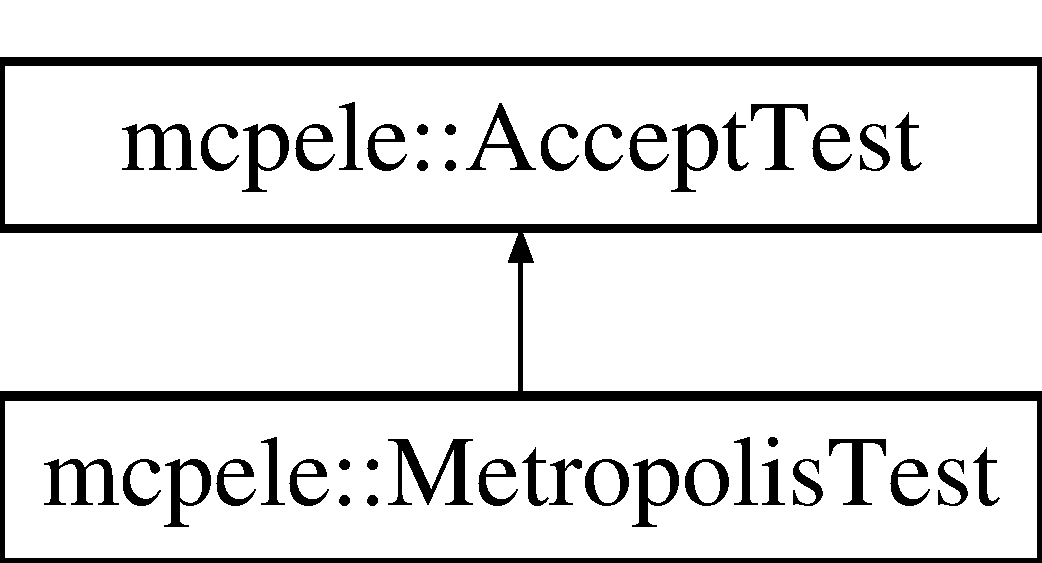
\includegraphics[height=2.000000cm]{classmcpele_1_1MetropolisTest}
\end{center}
\end{figure}
\subsection*{\-Public \-Member \-Functions}
\begin{DoxyCompactItemize}
\item 
\hyperlink{classmcpele_1_1MetropolisTest_a9cf4477f7ddfc2999178d99861f915a2}{\-Metropolis\-Test} (const size\-\_\-t rseed)
\item 
virtual \hyperlink{classmcpele_1_1MetropolisTest_a3c7b3df9ae8624eb3e4e4e2aa94249d0}{$\sim$\-Metropolis\-Test} ()
\item 
virtual bool \hyperlink{classmcpele_1_1MetropolisTest_ae59f0c208bedf4c8e2671c7150f8dcd7}{test} (pele\-::\-Array$<$ double $>$ \&trial\-\_\-coords, double trial\-\_\-energy, pele\-::\-Array$<$ double $>$ \&old\-\_\-coords, double old\-\_\-energy, double temperature, \hyperlink{classmcpele_1_1MC}{\-M\-C} $\ast$mc)
\item 
size\-\_\-t \hyperlink{classmcpele_1_1MetropolisTest_a8f02eef6939b2acc3d2b50af04248dcf}{get\-\_\-seed} () const 
\item 
void \hyperlink{classmcpele_1_1MetropolisTest_a6c1fe3e8acdeb71a806c94cf8318936b}{set\-\_\-generator\-\_\-seed} (const size\-\_\-t inp)
\end{DoxyCompactItemize}
\subsection*{\-Protected \-Attributes}
\begin{DoxyCompactItemize}
\item 
size\-\_\-t \hyperlink{classmcpele_1_1MetropolisTest_aa2973163ef6d8160e5f1d096cc7d4170}{m\-\_\-seed}
\item 
std\-::mt19937\-\_\-64 \hyperlink{classmcpele_1_1MetropolisTest_acf16d24f5b32afb1977c542e20dc23cf}{m\-\_\-generator}
\item 
std\-::uniform\-\_\-real\-\_\-distribution\*
$<$ double $>$ \hyperlink{classmcpele_1_1MetropolisTest_a98284c84912422d5846aef7f21772740}{m\-\_\-distribution}
\end{DoxyCompactItemize}


\subsection{\-Detailed \-Description}
\-The \-Metropolis acceptance criterion accepts each move with probability \[ P( x_{old} \Rightarrow x_{new}) = min \{ 1, \exp [- \beta (E_{new} - E_{old})] \} \] where $\beta$ is the reciprocal of the temperature 

\-Definition at line 24 of file metropolis\-\_\-test.\-h.



\subsection{\-Constructor \& \-Destructor \-Documentation}
\hypertarget{classmcpele_1_1MetropolisTest_a9cf4477f7ddfc2999178d99861f915a2}{\index{mcpele\-::\-Metropolis\-Test@{mcpele\-::\-Metropolis\-Test}!\-Metropolis\-Test@{\-Metropolis\-Test}}
\index{\-Metropolis\-Test@{\-Metropolis\-Test}!mcpele::MetropolisTest@{mcpele\-::\-Metropolis\-Test}}
\subsubsection[{\-Metropolis\-Test}]{\setlength{\rightskip}{0pt plus 5cm}{\bf mcpele\-::\-Metropolis\-Test\-::\-Metropolis\-Test} (
\begin{DoxyParamCaption}
\item[{const size\-\_\-t}]{rseed}
\end{DoxyParamCaption}
)}}\label{classmcpele_1_1MetropolisTest_a9cf4477f7ddfc2999178d99861f915a2}


\-Definition at line 10 of file metropolis\-\_\-test.\-cpp.

\hypertarget{classmcpele_1_1MetropolisTest_a3c7b3df9ae8624eb3e4e4e2aa94249d0}{\index{mcpele\-::\-Metropolis\-Test@{mcpele\-::\-Metropolis\-Test}!$\sim$\-Metropolis\-Test@{$\sim$\-Metropolis\-Test}}
\index{$\sim$\-Metropolis\-Test@{$\sim$\-Metropolis\-Test}!mcpele::MetropolisTest@{mcpele\-::\-Metropolis\-Test}}
\subsubsection[{$\sim$\-Metropolis\-Test}]{\setlength{\rightskip}{0pt plus 5cm}virtual {\bf mcpele\-::\-Metropolis\-Test\-::$\sim$\-Metropolis\-Test} (
\begin{DoxyParamCaption}
{}
\end{DoxyParamCaption}
)\hspace{0.3cm}{\ttfamily  \mbox{[}inline, virtual\mbox{]}}}}\label{classmcpele_1_1MetropolisTest_a3c7b3df9ae8624eb3e4e4e2aa94249d0}


\-Definition at line 31 of file metropolis\-\_\-test.\-h.



\subsection{\-Member \-Function \-Documentation}
\hypertarget{classmcpele_1_1MetropolisTest_a8f02eef6939b2acc3d2b50af04248dcf}{\index{mcpele\-::\-Metropolis\-Test@{mcpele\-::\-Metropolis\-Test}!get\-\_\-seed@{get\-\_\-seed}}
\index{get\-\_\-seed@{get\-\_\-seed}!mcpele::MetropolisTest@{mcpele\-::\-Metropolis\-Test}}
\subsubsection[{get\-\_\-seed}]{\setlength{\rightskip}{0pt plus 5cm}size\-\_\-t {\bf mcpele\-::\-Metropolis\-Test\-::get\-\_\-seed} (
\begin{DoxyParamCaption}
{}
\end{DoxyParamCaption}
) const\hspace{0.3cm}{\ttfamily  \mbox{[}inline\mbox{]}}}}\label{classmcpele_1_1MetropolisTest_a8f02eef6939b2acc3d2b50af04248dcf}


\-Definition at line 35 of file metropolis\-\_\-test.\-h.

\hypertarget{classmcpele_1_1MetropolisTest_a6c1fe3e8acdeb71a806c94cf8318936b}{\index{mcpele\-::\-Metropolis\-Test@{mcpele\-::\-Metropolis\-Test}!set\-\_\-generator\-\_\-seed@{set\-\_\-generator\-\_\-seed}}
\index{set\-\_\-generator\-\_\-seed@{set\-\_\-generator\-\_\-seed}!mcpele::MetropolisTest@{mcpele\-::\-Metropolis\-Test}}
\subsubsection[{set\-\_\-generator\-\_\-seed}]{\setlength{\rightskip}{0pt plus 5cm}void {\bf mcpele\-::\-Metropolis\-Test\-::set\-\_\-generator\-\_\-seed} (
\begin{DoxyParamCaption}
\item[{const size\-\_\-t}]{inp}
\end{DoxyParamCaption}
)\hspace{0.3cm}{\ttfamily  \mbox{[}inline\mbox{]}}}}\label{classmcpele_1_1MetropolisTest_a6c1fe3e8acdeb71a806c94cf8318936b}


\-Definition at line 36 of file metropolis\-\_\-test.\-h.

\hypertarget{classmcpele_1_1MetropolisTest_ae59f0c208bedf4c8e2671c7150f8dcd7}{\index{mcpele\-::\-Metropolis\-Test@{mcpele\-::\-Metropolis\-Test}!test@{test}}
\index{test@{test}!mcpele::MetropolisTest@{mcpele\-::\-Metropolis\-Test}}
\subsubsection[{test}]{\setlength{\rightskip}{0pt plus 5cm}bool {\bf mcpele\-::\-Metropolis\-Test\-::test} (
\begin{DoxyParamCaption}
\item[{pele\-::\-Array$<$ double $>$ \&}]{trial\-\_\-coords, }
\item[{double}]{trial\-\_\-energy, }
\item[{pele\-::\-Array$<$ double $>$ \&}]{old\-\_\-coords, }
\item[{double}]{old\-\_\-energy, }
\item[{double}]{temperature, }
\item[{{\bf \-M\-C} $\ast$}]{mc}
\end{DoxyParamCaption}
)\hspace{0.3cm}{\ttfamily  \mbox{[}virtual\mbox{]}}}}\label{classmcpele_1_1MetropolisTest_ae59f0c208bedf4c8e2671c7150f8dcd7}


\-Implements \hyperlink{classmcpele_1_1AcceptTest_ae2d9e2feaae60d49a35c7170f56f5d78}{mcpele\-::\-Accept\-Test}.



\-Definition at line 21 of file metropolis\-\_\-test.\-cpp.



\subsection{\-Member \-Data \-Documentation}
\hypertarget{classmcpele_1_1MetropolisTest_a98284c84912422d5846aef7f21772740}{\index{mcpele\-::\-Metropolis\-Test@{mcpele\-::\-Metropolis\-Test}!m\-\_\-distribution@{m\-\_\-distribution}}
\index{m\-\_\-distribution@{m\-\_\-distribution}!mcpele::MetropolisTest@{mcpele\-::\-Metropolis\-Test}}
\subsubsection[{m\-\_\-distribution}]{\setlength{\rightskip}{0pt plus 5cm}std\-::uniform\-\_\-real\-\_\-distribution$<$double$>$ {\bf mcpele\-::\-Metropolis\-Test\-::m\-\_\-distribution}\hspace{0.3cm}{\ttfamily  \mbox{[}protected\mbox{]}}}}\label{classmcpele_1_1MetropolisTest_a98284c84912422d5846aef7f21772740}


\-Definition at line 28 of file metropolis\-\_\-test.\-h.

\hypertarget{classmcpele_1_1MetropolisTest_acf16d24f5b32afb1977c542e20dc23cf}{\index{mcpele\-::\-Metropolis\-Test@{mcpele\-::\-Metropolis\-Test}!m\-\_\-generator@{m\-\_\-generator}}
\index{m\-\_\-generator@{m\-\_\-generator}!mcpele::MetropolisTest@{mcpele\-::\-Metropolis\-Test}}
\subsubsection[{m\-\_\-generator}]{\setlength{\rightskip}{0pt plus 5cm}std\-::mt19937\-\_\-64 {\bf mcpele\-::\-Metropolis\-Test\-::m\-\_\-generator}\hspace{0.3cm}{\ttfamily  \mbox{[}protected\mbox{]}}}}\label{classmcpele_1_1MetropolisTest_acf16d24f5b32afb1977c542e20dc23cf}


\-Definition at line 27 of file metropolis\-\_\-test.\-h.

\hypertarget{classmcpele_1_1MetropolisTest_aa2973163ef6d8160e5f1d096cc7d4170}{\index{mcpele\-::\-Metropolis\-Test@{mcpele\-::\-Metropolis\-Test}!m\-\_\-seed@{m\-\_\-seed}}
\index{m\-\_\-seed@{m\-\_\-seed}!mcpele::MetropolisTest@{mcpele\-::\-Metropolis\-Test}}
\subsubsection[{m\-\_\-seed}]{\setlength{\rightskip}{0pt plus 5cm}size\-\_\-t {\bf mcpele\-::\-Metropolis\-Test\-::m\-\_\-seed}\hspace{0.3cm}{\ttfamily  \mbox{[}protected\mbox{]}}}}\label{classmcpele_1_1MetropolisTest_aa2973163ef6d8160e5f1d096cc7d4170}


\-Definition at line 26 of file metropolis\-\_\-test.\-h.



\-The documentation for this class was generated from the following files\-:\begin{DoxyCompactItemize}
\item 
mcpele/\hyperlink{metropolis__test_8h}{metropolis\-\_\-test.\-h}\item 
\hyperlink{metropolis__test_8cpp}{metropolis\-\_\-test.\-cpp}\end{DoxyCompactItemize}

\hypertarget{classmcpele_1_1Moments}{\section{mcpele\-:\-:\-Moments \-Class \-Reference}
\label{classmcpele_1_1Moments}\index{mcpele\-::\-Moments@{mcpele\-::\-Moments}}
}


{\ttfamily \#include $<$histogram.\-h$>$}

\subsection*{\-Public \-Types}
\begin{DoxyCompactItemize}
\item 
typedef double \hyperlink{classmcpele_1_1Moments_a2dc6e59f3fa3498e008c64955a693e4b}{data\-\_\-t}
\item 
typedef size\-\_\-t \hyperlink{classmcpele_1_1Moments_a73dc5d511f63d1f4769d05bbc535f24c}{index\-\_\-t}
\end{DoxyCompactItemize}
\subsection*{\-Public \-Member \-Functions}
\begin{DoxyCompactItemize}
\item 
\hyperlink{classmcpele_1_1Moments_ad40f97eac46ca595e759f6d2e249b2ad}{\-Moments} ()
\item 
void \hyperlink{classmcpele_1_1Moments_a4013c89a1d84431b62ca3ad7d32d5278}{update} (const \hyperlink{classmcpele_1_1Moments_a2dc6e59f3fa3498e008c64955a693e4b}{data\-\_\-t} input)
\item 
void \hyperlink{classmcpele_1_1Moments_a6526753dd1c2be0863f7d02ddf8573b4}{replace} (const \hyperlink{classmcpele_1_1Moments_a2dc6e59f3fa3498e008c64955a693e4b}{data\-\_\-t} old\-\_\-data, const \hyperlink{classmcpele_1_1Moments_a2dc6e59f3fa3498e008c64955a693e4b}{data\-\_\-t} new\-\_\-data)
\item 
void \hyperlink{classmcpele_1_1Moments_aae097b850d24e7e969a0b69e0590cdfa}{operator()} (const \hyperlink{classmcpele_1_1Moments_a2dc6e59f3fa3498e008c64955a693e4b}{data\-\_\-t} input)
\item 
\hyperlink{classmcpele_1_1Moments_a73dc5d511f63d1f4769d05bbc535f24c}{index\-\_\-t} \hyperlink{classmcpele_1_1Moments_afb38f4e5675d4e3ecded24153d64f69b}{count} () const 
\item 
\hyperlink{classmcpele_1_1Moments_a2dc6e59f3fa3498e008c64955a693e4b}{data\-\_\-t} \hyperlink{classmcpele_1_1Moments_a1707a2b086488a643deb51e06bdf8c48}{mean} () const 
\item 
\hyperlink{classmcpele_1_1Moments_a2dc6e59f3fa3498e008c64955a693e4b}{data\-\_\-t} \hyperlink{classmcpele_1_1Moments_a1fffc728d29b659f9f8c6438168f794d}{variance} () const 
\item 
\hyperlink{classmcpele_1_1Moments_a2dc6e59f3fa3498e008c64955a693e4b}{data\-\_\-t} \hyperlink{classmcpele_1_1Moments_afe797a35a1e551a057348de77807d34e}{std} () const 
\end{DoxyCompactItemize}


\subsection{\-Detailed \-Description}


\-Definition at line 26 of file histogram.\-h.



\subsection{\-Member \-Typedef \-Documentation}
\hypertarget{classmcpele_1_1Moments_a2dc6e59f3fa3498e008c64955a693e4b}{\index{mcpele\-::\-Moments@{mcpele\-::\-Moments}!data\-\_\-t@{data\-\_\-t}}
\index{data\-\_\-t@{data\-\_\-t}!mcpele::Moments@{mcpele\-::\-Moments}}
\subsubsection[{data\-\_\-t}]{\setlength{\rightskip}{0pt plus 5cm}typedef double {\bf mcpele\-::\-Moments\-::data\-\_\-t}}}\label{classmcpele_1_1Moments_a2dc6e59f3fa3498e008c64955a693e4b}


\-Definition at line 28 of file histogram.\-h.

\hypertarget{classmcpele_1_1Moments_a73dc5d511f63d1f4769d05bbc535f24c}{\index{mcpele\-::\-Moments@{mcpele\-::\-Moments}!index\-\_\-t@{index\-\_\-t}}
\index{index\-\_\-t@{index\-\_\-t}!mcpele::Moments@{mcpele\-::\-Moments}}
\subsubsection[{index\-\_\-t}]{\setlength{\rightskip}{0pt plus 5cm}typedef size\-\_\-t {\bf mcpele\-::\-Moments\-::index\-\_\-t}}}\label{classmcpele_1_1Moments_a73dc5d511f63d1f4769d05bbc535f24c}


\-Definition at line 29 of file histogram.\-h.



\subsection{\-Constructor \& \-Destructor \-Documentation}
\hypertarget{classmcpele_1_1Moments_ad40f97eac46ca595e759f6d2e249b2ad}{\index{mcpele\-::\-Moments@{mcpele\-::\-Moments}!\-Moments@{\-Moments}}
\index{\-Moments@{\-Moments}!mcpele::Moments@{mcpele\-::\-Moments}}
\subsubsection[{\-Moments}]{\setlength{\rightskip}{0pt plus 5cm}{\bf mcpele\-::\-Moments\-::\-Moments} (
\begin{DoxyParamCaption}
{}
\end{DoxyParamCaption}
)\hspace{0.3cm}{\ttfamily  \mbox{[}inline\mbox{]}}}}\label{classmcpele_1_1Moments_ad40f97eac46ca595e759f6d2e249b2ad}


\-Definition at line 35 of file histogram.\-h.



\subsection{\-Member \-Function \-Documentation}
\hypertarget{classmcpele_1_1Moments_afb38f4e5675d4e3ecded24153d64f69b}{\index{mcpele\-::\-Moments@{mcpele\-::\-Moments}!count@{count}}
\index{count@{count}!mcpele::Moments@{mcpele\-::\-Moments}}
\subsubsection[{count}]{\setlength{\rightskip}{0pt plus 5cm}{\bf index\-\_\-t} {\bf mcpele\-::\-Moments\-::count} (
\begin{DoxyParamCaption}
{}
\end{DoxyParamCaption}
) const\hspace{0.3cm}{\ttfamily  \mbox{[}inline\mbox{]}}}}\label{classmcpele_1_1Moments_afb38f4e5675d4e3ecded24153d64f69b}


\-Definition at line 58 of file histogram.\-h.

\hypertarget{classmcpele_1_1Moments_a1707a2b086488a643deb51e06bdf8c48}{\index{mcpele\-::\-Moments@{mcpele\-::\-Moments}!mean@{mean}}
\index{mean@{mean}!mcpele::Moments@{mcpele\-::\-Moments}}
\subsubsection[{mean}]{\setlength{\rightskip}{0pt plus 5cm}{\bf data\-\_\-t} {\bf mcpele\-::\-Moments\-::mean} (
\begin{DoxyParamCaption}
{}
\end{DoxyParamCaption}
) const\hspace{0.3cm}{\ttfamily  \mbox{[}inline\mbox{]}}}}\label{classmcpele_1_1Moments_a1707a2b086488a643deb51e06bdf8c48}


\-Definition at line 59 of file histogram.\-h.

\hypertarget{classmcpele_1_1Moments_aae097b850d24e7e969a0b69e0590cdfa}{\index{mcpele\-::\-Moments@{mcpele\-::\-Moments}!operator()@{operator()}}
\index{operator()@{operator()}!mcpele::Moments@{mcpele\-::\-Moments}}
\subsubsection[{operator()}]{\setlength{\rightskip}{0pt plus 5cm}void mcpele\-::\-Moments\-::operator() (
\begin{DoxyParamCaption}
\item[{const {\bf data\-\_\-t}}]{input}
\end{DoxyParamCaption}
)\hspace{0.3cm}{\ttfamily  \mbox{[}inline\mbox{]}}}}\label{classmcpele_1_1Moments_aae097b850d24e7e969a0b69e0590cdfa}


\-Definition at line 57 of file histogram.\-h.

\hypertarget{classmcpele_1_1Moments_a6526753dd1c2be0863f7d02ddf8573b4}{\index{mcpele\-::\-Moments@{mcpele\-::\-Moments}!replace@{replace}}
\index{replace@{replace}!mcpele::Moments@{mcpele\-::\-Moments}}
\subsubsection[{replace}]{\setlength{\rightskip}{0pt plus 5cm}void {\bf mcpele\-::\-Moments\-::replace} (
\begin{DoxyParamCaption}
\item[{const {\bf data\-\_\-t}}]{old\-\_\-data, }
\item[{const {\bf data\-\_\-t}}]{new\-\_\-data}
\end{DoxyParamCaption}
)\hspace{0.3cm}{\ttfamily  \mbox{[}inline\mbox{]}}}}\label{classmcpele_1_1Moments_a6526753dd1c2be0863f7d02ddf8573b4}
replace a data point with another one 

\-Definition at line 52 of file histogram.\-h.

\hypertarget{classmcpele_1_1Moments_afe797a35a1e551a057348de77807d34e}{\index{mcpele\-::\-Moments@{mcpele\-::\-Moments}!std@{std}}
\index{std@{std}!mcpele::Moments@{mcpele\-::\-Moments}}
\subsubsection[{std}]{\setlength{\rightskip}{0pt plus 5cm}{\bf data\-\_\-t} {\bf mcpele\-::\-Moments\-::std} (
\begin{DoxyParamCaption}
{}
\end{DoxyParamCaption}
) const\hspace{0.3cm}{\ttfamily  \mbox{[}inline\mbox{]}}}}\label{classmcpele_1_1Moments_afe797a35a1e551a057348de77807d34e}


\-Definition at line 61 of file histogram.\-h.

\hypertarget{classmcpele_1_1Moments_a4013c89a1d84431b62ca3ad7d32d5278}{\index{mcpele\-::\-Moments@{mcpele\-::\-Moments}!update@{update}}
\index{update@{update}!mcpele::Moments@{mcpele\-::\-Moments}}
\subsubsection[{update}]{\setlength{\rightskip}{0pt plus 5cm}void {\bf mcpele\-::\-Moments\-::update} (
\begin{DoxyParamCaption}
\item[{const {\bf data\-\_\-t}}]{input}
\end{DoxyParamCaption}
)\hspace{0.3cm}{\ttfamily  \mbox{[}inline\mbox{]}}}}\label{classmcpele_1_1Moments_a4013c89a1d84431b62ca3ad7d32d5278}


\-Definition at line 40 of file histogram.\-h.

\hypertarget{classmcpele_1_1Moments_a1fffc728d29b659f9f8c6438168f794d}{\index{mcpele\-::\-Moments@{mcpele\-::\-Moments}!variance@{variance}}
\index{variance@{variance}!mcpele::Moments@{mcpele\-::\-Moments}}
\subsubsection[{variance}]{\setlength{\rightskip}{0pt plus 5cm}{\bf data\-\_\-t} {\bf mcpele\-::\-Moments\-::variance} (
\begin{DoxyParamCaption}
{}
\end{DoxyParamCaption}
) const\hspace{0.3cm}{\ttfamily  \mbox{[}inline\mbox{]}}}}\label{classmcpele_1_1Moments_a1fffc728d29b659f9f8c6438168f794d}


\-Definition at line 60 of file histogram.\-h.



\-The documentation for this class was generated from the following file\-:\begin{DoxyCompactItemize}
\item 
mcpele/\hyperlink{histogram_8h}{histogram.\-h}\end{DoxyCompactItemize}

\hypertarget{classmcpele_1_1MovingAverageAcc}{\section{mcpele\-:\-:\-Moving\-Average\-Acc \-Class \-Reference}
\label{classmcpele_1_1MovingAverageAcc}\index{mcpele\-::\-Moving\-Average\-Acc@{mcpele\-::\-Moving\-Average\-Acc}}
}


{\ttfamily \#include $<$moving\-\_\-average.\-h$>$}

\subsection*{\-Public \-Member \-Functions}
\begin{DoxyCompactItemize}
\item 
\hyperlink{classmcpele_1_1MovingAverageAcc_ae6fec71cbafebc71e9a905899a7896de}{\-Moving\-Average\-Acc} (const std\-::vector$<$ double $>$ \&time\-\_\-series, const size\-\_\-t nr\-\_\-steps\-\_\-total, const size\-\_\-t nr\-\_\-steps\-\_\-ma)
\item 
double \hyperlink{classmcpele_1_1MovingAverageAcc_a9425234b23392b4e5bba42fc97d16003}{get\-\_\-mean} () const 
\item 
double \hyperlink{classmcpele_1_1MovingAverageAcc_a773b8ca120bbdf022d2bc47a0675fae0}{get\-\_\-variance} () const 
\item 
size\-\_\-t \hyperlink{classmcpele_1_1MovingAverageAcc_a5445445958b84d53fb79de34c755b989}{get\-\_\-nr\-\_\-steps\-\_\-ma} () const 
\item 
void \hyperlink{classmcpele_1_1MovingAverageAcc_a9e2cdb6a33be91c777151422405f7e0e}{shift\-\_\-right} ()
\item 
void \hyperlink{classmcpele_1_1MovingAverageAcc_ac949ea89cec25587bcb3ba0d9a07c3fb}{reset} ()
\end{DoxyCompactItemize}


\subsection{\-Detailed \-Description}
\-Computes moving averages of time series. \-Reference to time series, from small to large times, is in m\-\_\-time\-\_\-series. \-Assume that one wants to compute moving averages for the rightmost (latest) m\-\_\-nr\-\_\-steps\-\_\-total elements of the time series. \-The number of time series steps that go into one moving average is m\-\_\-nr\-\_\-steps\-\_\-ma. \-The number of different moving averages that one can compute, given these two parameters (m\-\_\-nr\-\_\-steps\-\_\-total and m\-\_\-window\-\_\-size) is m\-\_\-nr\-\_\-steps\-\_\-ma. \-Moving average is initialised to the leftmost moving average. \-After that \hyperlink{classmcpele_1_1MovingAverageAcc_a9e2cdb6a33be91c777151422405f7e0e}{shift\-\_\-right()} moves the moving average window one time series step further to the right (to the future). \-In case \hyperlink{classmcpele_1_1MovingAverageAcc_a9e2cdb6a33be91c777151422405f7e0e}{shift\-\_\-right()} reaches the last step in the time series, the moving average window returns to the initial position. 

\-Definition at line 26 of file moving\-\_\-average.\-h.



\subsection{\-Constructor \& \-Destructor \-Documentation}
\hypertarget{classmcpele_1_1MovingAverageAcc_ae6fec71cbafebc71e9a905899a7896de}{\index{mcpele\-::\-Moving\-Average\-Acc@{mcpele\-::\-Moving\-Average\-Acc}!\-Moving\-Average\-Acc@{\-Moving\-Average\-Acc}}
\index{\-Moving\-Average\-Acc@{\-Moving\-Average\-Acc}!mcpele::MovingAverageAcc@{mcpele\-::\-Moving\-Average\-Acc}}
\subsubsection[{\-Moving\-Average\-Acc}]{\setlength{\rightskip}{0pt plus 5cm}{\bf mcpele\-::\-Moving\-Average\-Acc\-::\-Moving\-Average\-Acc} (
\begin{DoxyParamCaption}
\item[{const std\-::vector$<$ double $>$ \&}]{time\-\_\-series, }
\item[{const size\-\_\-t}]{nr\-\_\-steps\-\_\-total, }
\item[{const size\-\_\-t}]{nr\-\_\-steps\-\_\-ma}
\end{DoxyParamCaption}
)\hspace{0.3cm}{\ttfamily  \mbox{[}inline\mbox{]}}}}\label{classmcpele_1_1MovingAverageAcc_ae6fec71cbafebc71e9a905899a7896de}


\-Definition at line 36 of file moving\-\_\-average.\-h.



\subsection{\-Member \-Function \-Documentation}
\hypertarget{classmcpele_1_1MovingAverageAcc_a9425234b23392b4e5bba42fc97d16003}{\index{mcpele\-::\-Moving\-Average\-Acc@{mcpele\-::\-Moving\-Average\-Acc}!get\-\_\-mean@{get\-\_\-mean}}
\index{get\-\_\-mean@{get\-\_\-mean}!mcpele::MovingAverageAcc@{mcpele\-::\-Moving\-Average\-Acc}}
\subsubsection[{get\-\_\-mean}]{\setlength{\rightskip}{0pt plus 5cm}double {\bf mcpele\-::\-Moving\-Average\-Acc\-::get\-\_\-mean} (
\begin{DoxyParamCaption}
{}
\end{DoxyParamCaption}
) const\hspace{0.3cm}{\ttfamily  \mbox{[}inline\mbox{]}}}}\label{classmcpele_1_1MovingAverageAcc_a9425234b23392b4e5bba42fc97d16003}


\-Definition at line 56 of file moving\-\_\-average.\-h.

\hypertarget{classmcpele_1_1MovingAverageAcc_a5445445958b84d53fb79de34c755b989}{\index{mcpele\-::\-Moving\-Average\-Acc@{mcpele\-::\-Moving\-Average\-Acc}!get\-\_\-nr\-\_\-steps\-\_\-ma@{get\-\_\-nr\-\_\-steps\-\_\-ma}}
\index{get\-\_\-nr\-\_\-steps\-\_\-ma@{get\-\_\-nr\-\_\-steps\-\_\-ma}!mcpele::MovingAverageAcc@{mcpele\-::\-Moving\-Average\-Acc}}
\subsubsection[{get\-\_\-nr\-\_\-steps\-\_\-ma}]{\setlength{\rightskip}{0pt plus 5cm}size\-\_\-t {\bf mcpele\-::\-Moving\-Average\-Acc\-::get\-\_\-nr\-\_\-steps\-\_\-ma} (
\begin{DoxyParamCaption}
{}
\end{DoxyParamCaption}
) const\hspace{0.3cm}{\ttfamily  \mbox{[}inline\mbox{]}}}}\label{classmcpele_1_1MovingAverageAcc_a5445445958b84d53fb79de34c755b989}


\-Definition at line 58 of file moving\-\_\-average.\-h.

\hypertarget{classmcpele_1_1MovingAverageAcc_a773b8ca120bbdf022d2bc47a0675fae0}{\index{mcpele\-::\-Moving\-Average\-Acc@{mcpele\-::\-Moving\-Average\-Acc}!get\-\_\-variance@{get\-\_\-variance}}
\index{get\-\_\-variance@{get\-\_\-variance}!mcpele::MovingAverageAcc@{mcpele\-::\-Moving\-Average\-Acc}}
\subsubsection[{get\-\_\-variance}]{\setlength{\rightskip}{0pt plus 5cm}double {\bf mcpele\-::\-Moving\-Average\-Acc\-::get\-\_\-variance} (
\begin{DoxyParamCaption}
{}
\end{DoxyParamCaption}
) const\hspace{0.3cm}{\ttfamily  \mbox{[}inline\mbox{]}}}}\label{classmcpele_1_1MovingAverageAcc_a773b8ca120bbdf022d2bc47a0675fae0}


\-Definition at line 57 of file moving\-\_\-average.\-h.

\hypertarget{classmcpele_1_1MovingAverageAcc_ac949ea89cec25587bcb3ba0d9a07c3fb}{\index{mcpele\-::\-Moving\-Average\-Acc@{mcpele\-::\-Moving\-Average\-Acc}!reset@{reset}}
\index{reset@{reset}!mcpele::MovingAverageAcc@{mcpele\-::\-Moving\-Average\-Acc}}
\subsubsection[{reset}]{\setlength{\rightskip}{0pt plus 5cm}void {\bf mcpele\-::\-Moving\-Average\-Acc\-::reset} (
\begin{DoxyParamCaption}
{}
\end{DoxyParamCaption}
)\hspace{0.3cm}{\ttfamily  \mbox{[}inline\mbox{]}}}}\label{classmcpele_1_1MovingAverageAcc_ac949ea89cec25587bcb3ba0d9a07c3fb}


\-Definition at line 70 of file moving\-\_\-average.\-h.

\hypertarget{classmcpele_1_1MovingAverageAcc_a9e2cdb6a33be91c777151422405f7e0e}{\index{mcpele\-::\-Moving\-Average\-Acc@{mcpele\-::\-Moving\-Average\-Acc}!shift\-\_\-right@{shift\-\_\-right}}
\index{shift\-\_\-right@{shift\-\_\-right}!mcpele::MovingAverageAcc@{mcpele\-::\-Moving\-Average\-Acc}}
\subsubsection[{shift\-\_\-right}]{\setlength{\rightskip}{0pt plus 5cm}void {\bf mcpele\-::\-Moving\-Average\-Acc\-::shift\-\_\-right} (
\begin{DoxyParamCaption}
{}
\end{DoxyParamCaption}
)\hspace{0.3cm}{\ttfamily  \mbox{[}inline\mbox{]}}}}\label{classmcpele_1_1MovingAverageAcc_a9e2cdb6a33be91c777151422405f7e0e}


\-Definition at line 59 of file moving\-\_\-average.\-h.



\-The documentation for this class was generated from the following file\-:\begin{DoxyCompactItemize}
\item 
mcpele/\hyperlink{moving__average_8h}{moving\-\_\-average.\-h}\end{DoxyCompactItemize}

\hypertarget{classmcpele_1_1PairDistHistogram}{\section{mcpele\-:\-:\-Pair\-Dist\-Histogram$<$ \-B\-O\-X\-D\-I\-M $>$ \-Class \-Template \-Reference}
\label{classmcpele_1_1PairDistHistogram}\index{mcpele\-::\-Pair\-Dist\-Histogram$<$ B\-O\-X\-D\-I\-M $>$@{mcpele\-::\-Pair\-Dist\-Histogram$<$ B\-O\-X\-D\-I\-M $>$}}
}


{\ttfamily \#include $<$pair\-\_\-dist\-\_\-histogram.\-h$>$}

\subsection*{\-Public \-Member \-Functions}
\begin{DoxyCompactItemize}
\item 
\hyperlink{classmcpele_1_1PairDistHistogram_a2eb2e7d4fe32c03f17f85ea18373af1c}{\-Pair\-Dist\-Histogram} (pele\-::\-Array$<$ double $>$ boxvector, const size\-\_\-t nr\-\_\-bins)
\item 
virtual \hyperlink{classmcpele_1_1PairDistHistogram_aa9e464547fc961cb8ec394331369aa55}{$\sim$\-Pair\-Dist\-Histogram} ()
\item 
void \hyperlink{classmcpele_1_1PairDistHistogram_aed454da4feb9525c05fa05389dfa875e}{add\-\_\-configuration} (pele\-::\-Array$<$ double $>$ coords)
\item 
void \hyperlink{classmcpele_1_1PairDistHistogram_afc8c7d70c8fd97c995ff1bcbfb1d2a41}{add\-\_\-distance} (const size\-\_\-t i, const size\-\_\-t j, const double $\ast$coor)
\item 
double \hyperlink{classmcpele_1_1PairDistHistogram_a60dbf068f7b45fa2a4ba59eef078705b}{volume\-\_\-nball} (const double radius, const size\-\_\-t ndim) const 
\item 
std\-::vector$<$ double $>$ \hyperlink{classmcpele_1_1PairDistHistogram_a00a321092cf3d428b36c4ea0695995ac}{get\-\_\-vecdata\-\_\-r} () const 
\item 
std\-::vector$<$ double $>$ \hyperlink{classmcpele_1_1PairDistHistogram_ac5a27c5e7329ac64829fc16c92fb911c}{get\-\_\-vecdata\-\_\-gr} (const double number\-\_\-density, const size\-\_\-t nr\-\_\-particles) const 
\end{DoxyCompactItemize}


\subsection{\-Detailed \-Description}
\subsubsection*{template$<$size\-\_\-t \-B\-O\-X\-D\-I\-M$>$class mcpele\-::\-Pair\-Dist\-Histogram$<$ B\-O\-X\-D\-I\-M $>$}



\-Definition at line 16 of file pair\-\_\-dist\-\_\-histogram.\-h.



\subsection{\-Constructor \& \-Destructor \-Documentation}
\hypertarget{classmcpele_1_1PairDistHistogram_a2eb2e7d4fe32c03f17f85ea18373af1c}{\index{mcpele\-::\-Pair\-Dist\-Histogram@{mcpele\-::\-Pair\-Dist\-Histogram}!\-Pair\-Dist\-Histogram@{\-Pair\-Dist\-Histogram}}
\index{\-Pair\-Dist\-Histogram@{\-Pair\-Dist\-Histogram}!mcpele::PairDistHistogram@{mcpele\-::\-Pair\-Dist\-Histogram}}
\subsubsection[{\-Pair\-Dist\-Histogram}]{\setlength{\rightskip}{0pt plus 5cm}template$<$size\-\_\-t \-B\-O\-X\-D\-I\-M$>$ {\bf mcpele\-::\-Pair\-Dist\-Histogram}$<$ \-B\-O\-X\-D\-I\-M $>$\-::{\bf \-Pair\-Dist\-Histogram} (
\begin{DoxyParamCaption}
\item[{pele\-::\-Array$<$ double $>$}]{boxvector, }
\item[{const size\-\_\-t}]{nr\-\_\-bins}
\end{DoxyParamCaption}
)\hspace{0.3cm}{\ttfamily  \mbox{[}inline\mbox{]}}}}\label{classmcpele_1_1PairDistHistogram_a2eb2e7d4fe32c03f17f85ea18373af1c}


\-Definition at line 26 of file pair\-\_\-dist\-\_\-histogram.\-h.

\hypertarget{classmcpele_1_1PairDistHistogram_aa9e464547fc961cb8ec394331369aa55}{\index{mcpele\-::\-Pair\-Dist\-Histogram@{mcpele\-::\-Pair\-Dist\-Histogram}!$\sim$\-Pair\-Dist\-Histogram@{$\sim$\-Pair\-Dist\-Histogram}}
\index{$\sim$\-Pair\-Dist\-Histogram@{$\sim$\-Pair\-Dist\-Histogram}!mcpele::PairDistHistogram@{mcpele\-::\-Pair\-Dist\-Histogram}}
\subsubsection[{$\sim$\-Pair\-Dist\-Histogram}]{\setlength{\rightskip}{0pt plus 5cm}template$<$size\-\_\-t \-B\-O\-X\-D\-I\-M$>$ virtual {\bf mcpele\-::\-Pair\-Dist\-Histogram}$<$ \-B\-O\-X\-D\-I\-M $>$\-::$\sim${\bf \-Pair\-Dist\-Histogram} (
\begin{DoxyParamCaption}
{}
\end{DoxyParamCaption}
)\hspace{0.3cm}{\ttfamily  \mbox{[}inline, virtual\mbox{]}}}}\label{classmcpele_1_1PairDistHistogram_aa9e464547fc961cb8ec394331369aa55}


\-Definition at line 39 of file pair\-\_\-dist\-\_\-histogram.\-h.



\subsection{\-Member \-Function \-Documentation}
\hypertarget{classmcpele_1_1PairDistHistogram_aed454da4feb9525c05fa05389dfa875e}{\index{mcpele\-::\-Pair\-Dist\-Histogram@{mcpele\-::\-Pair\-Dist\-Histogram}!add\-\_\-configuration@{add\-\_\-configuration}}
\index{add\-\_\-configuration@{add\-\_\-configuration}!mcpele::PairDistHistogram@{mcpele\-::\-Pair\-Dist\-Histogram}}
\subsubsection[{add\-\_\-configuration}]{\setlength{\rightskip}{0pt plus 5cm}template$<$size\-\_\-t \-B\-O\-X\-D\-I\-M$>$ void {\bf mcpele\-::\-Pair\-Dist\-Histogram}$<$ \-B\-O\-X\-D\-I\-M $>$\-::{\bf add\-\_\-configuration} (
\begin{DoxyParamCaption}
\item[{pele\-::\-Array$<$ double $>$}]{coords}
\end{DoxyParamCaption}
)\hspace{0.3cm}{\ttfamily  \mbox{[}inline\mbox{]}}}}\label{classmcpele_1_1PairDistHistogram_aed454da4feb9525c05fa05389dfa875e}


\-Definition at line 40 of file pair\-\_\-dist\-\_\-histogram.\-h.

\hypertarget{classmcpele_1_1PairDistHistogram_afc8c7d70c8fd97c995ff1bcbfb1d2a41}{\index{mcpele\-::\-Pair\-Dist\-Histogram@{mcpele\-::\-Pair\-Dist\-Histogram}!add\-\_\-distance@{add\-\_\-distance}}
\index{add\-\_\-distance@{add\-\_\-distance}!mcpele::PairDistHistogram@{mcpele\-::\-Pair\-Dist\-Histogram}}
\subsubsection[{add\-\_\-distance}]{\setlength{\rightskip}{0pt plus 5cm}template$<$size\-\_\-t \-B\-O\-X\-D\-I\-M$>$ void {\bf mcpele\-::\-Pair\-Dist\-Histogram}$<$ \-B\-O\-X\-D\-I\-M $>$\-::{\bf add\-\_\-distance} (
\begin{DoxyParamCaption}
\item[{const size\-\_\-t}]{i, }
\item[{const size\-\_\-t}]{j, }
\item[{const double $\ast$}]{coor}
\end{DoxyParamCaption}
)\hspace{0.3cm}{\ttfamily  \mbox{[}inline\mbox{]}}}}\label{classmcpele_1_1PairDistHistogram_afc8c7d70c8fd97c995ff1bcbfb1d2a41}


\-Definition at line 50 of file pair\-\_\-dist\-\_\-histogram.\-h.

\hypertarget{classmcpele_1_1PairDistHistogram_ac5a27c5e7329ac64829fc16c92fb911c}{\index{mcpele\-::\-Pair\-Dist\-Histogram@{mcpele\-::\-Pair\-Dist\-Histogram}!get\-\_\-vecdata\-\_\-gr@{get\-\_\-vecdata\-\_\-gr}}
\index{get\-\_\-vecdata\-\_\-gr@{get\-\_\-vecdata\-\_\-gr}!mcpele::PairDistHistogram@{mcpele\-::\-Pair\-Dist\-Histogram}}
\subsubsection[{get\-\_\-vecdata\-\_\-gr}]{\setlength{\rightskip}{0pt plus 5cm}template$<$size\-\_\-t \-B\-O\-X\-D\-I\-M$>$ std\-::vector$<$double$>$ {\bf mcpele\-::\-Pair\-Dist\-Histogram}$<$ \-B\-O\-X\-D\-I\-M $>$\-::{\bf get\-\_\-vecdata\-\_\-gr} (
\begin{DoxyParamCaption}
\item[{const double}]{number\-\_\-density, }
\item[{const size\-\_\-t}]{nr\-\_\-particles}
\end{DoxyParamCaption}
) const\hspace{0.3cm}{\ttfamily  \mbox{[}inline\mbox{]}}}}\label{classmcpele_1_1PairDistHistogram_ac5a27c5e7329ac64829fc16c92fb911c}


\-Definition at line 80 of file pair\-\_\-dist\-\_\-histogram.\-h.

\hypertarget{classmcpele_1_1PairDistHistogram_a00a321092cf3d428b36c4ea0695995ac}{\index{mcpele\-::\-Pair\-Dist\-Histogram@{mcpele\-::\-Pair\-Dist\-Histogram}!get\-\_\-vecdata\-\_\-r@{get\-\_\-vecdata\-\_\-r}}
\index{get\-\_\-vecdata\-\_\-r@{get\-\_\-vecdata\-\_\-r}!mcpele::PairDistHistogram@{mcpele\-::\-Pair\-Dist\-Histogram}}
\subsubsection[{get\-\_\-vecdata\-\_\-r}]{\setlength{\rightskip}{0pt plus 5cm}template$<$size\-\_\-t \-B\-O\-X\-D\-I\-M$>$ std\-::vector$<$double$>$ {\bf mcpele\-::\-Pair\-Dist\-Histogram}$<$ \-B\-O\-X\-D\-I\-M $>$\-::{\bf get\-\_\-vecdata\-\_\-r} (
\begin{DoxyParamCaption}
{}
\end{DoxyParamCaption}
) const\hspace{0.3cm}{\ttfamily  \mbox{[}inline\mbox{]}}}}\label{classmcpele_1_1PairDistHistogram_a00a321092cf3d428b36c4ea0695995ac}


\-Definition at line 71 of file pair\-\_\-dist\-\_\-histogram.\-h.

\hypertarget{classmcpele_1_1PairDistHistogram_a60dbf068f7b45fa2a4ba59eef078705b}{\index{mcpele\-::\-Pair\-Dist\-Histogram@{mcpele\-::\-Pair\-Dist\-Histogram}!volume\-\_\-nball@{volume\-\_\-nball}}
\index{volume\-\_\-nball@{volume\-\_\-nball}!mcpele::PairDistHistogram@{mcpele\-::\-Pair\-Dist\-Histogram}}
\subsubsection[{volume\-\_\-nball}]{\setlength{\rightskip}{0pt plus 5cm}template$<$size\-\_\-t \-B\-O\-X\-D\-I\-M$>$ double {\bf mcpele\-::\-Pair\-Dist\-Histogram}$<$ \-B\-O\-X\-D\-I\-M $>$\-::{\bf volume\-\_\-nball} (
\begin{DoxyParamCaption}
\item[{const double}]{radius, }
\item[{const size\-\_\-t}]{ndim}
\end{DoxyParamCaption}
) const\hspace{0.3cm}{\ttfamily  \mbox{[}inline\mbox{]}}}}\label{classmcpele_1_1PairDistHistogram_a60dbf068f7b45fa2a4ba59eef078705b}


\-Definition at line 67 of file pair\-\_\-dist\-\_\-histogram.\-h.



\-The documentation for this class was generated from the following file\-:\begin{DoxyCompactItemize}
\item 
mcpele/\hyperlink{pair__dist__histogram_8h}{pair\-\_\-dist\-\_\-histogram.\-h}\end{DoxyCompactItemize}

\hypertarget{classmcpele_1_1ParticlePairSwap}{\section{mcpele\-:\-:\-Particle\-Pair\-Swap \-Class \-Reference}
\label{classmcpele_1_1ParticlePairSwap}\index{mcpele\-::\-Particle\-Pair\-Swap@{mcpele\-::\-Particle\-Pair\-Swap}}
}


{\ttfamily \#include $<$particle\-\_\-pair\-\_\-swap.\-h$>$}

\-Inheritance diagram for mcpele\-:\-:\-Particle\-Pair\-Swap\-:\begin{figure}[H]
\begin{center}
\leavevmode
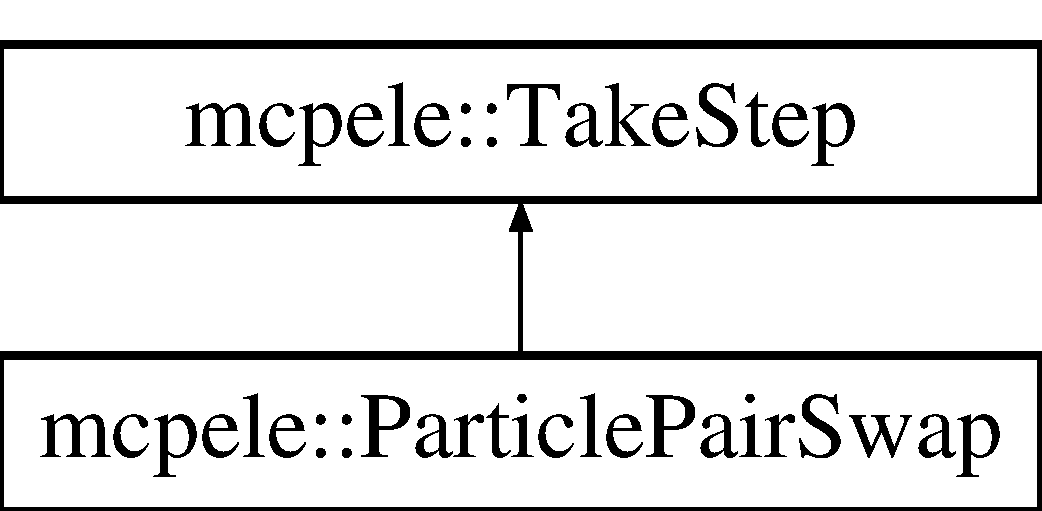
\includegraphics[height=2.000000cm]{classmcpele_1_1ParticlePairSwap}
\end{center}
\end{figure}
\subsection*{\-Public \-Member \-Functions}
\begin{DoxyCompactItemize}
\item 
virtual \hyperlink{classmcpele_1_1ParticlePairSwap_a391476c1f25fa3e194b69cfb542adea3}{$\sim$\-Particle\-Pair\-Swap} ()
\item 
\hyperlink{classmcpele_1_1ParticlePairSwap_a09aebe2a1c7a5e89be202def3bfded9f}{\-Particle\-Pair\-Swap} (const size\-\_\-t seed, const size\-\_\-t nr\-\_\-particles)
\item 
void \hyperlink{classmcpele_1_1ParticlePairSwap_ab4d35820381b34f5e4c993ad3817427b}{displace} (pele\-::\-Array$<$ double $>$ \&coords, \hyperlink{classmcpele_1_1MC}{\-M\-C} $\ast$mc)
\item 
void \hyperlink{classmcpele_1_1ParticlePairSwap_a075a55654c1cd9d6d80a361acc8014ed}{swap\-\_\-coordinates} (const size\-\_\-t particle\-\_\-a, const size\-\_\-t particle\-\_\-b, pele\-::\-Array$<$ double $>$ \&coords)
\item 
size\-\_\-t \hyperlink{classmcpele_1_1ParticlePairSwap_a1f3abbcf103328a91eeda411199fe478}{get\-\_\-seed} () const 
\item 
void \hyperlink{classmcpele_1_1ParticlePairSwap_a1142a8be79e9c872ab07f0f9995656fe}{set\-\_\-generator\-\_\-seed} (const size\-\_\-t inp)
\end{DoxyCompactItemize}


\subsection{\-Detailed \-Description}


\-Definition at line 10 of file particle\-\_\-pair\-\_\-swap.\-h.



\subsection{\-Constructor \& \-Destructor \-Documentation}
\hypertarget{classmcpele_1_1ParticlePairSwap_a391476c1f25fa3e194b69cfb542adea3}{\index{mcpele\-::\-Particle\-Pair\-Swap@{mcpele\-::\-Particle\-Pair\-Swap}!$\sim$\-Particle\-Pair\-Swap@{$\sim$\-Particle\-Pair\-Swap}}
\index{$\sim$\-Particle\-Pair\-Swap@{$\sim$\-Particle\-Pair\-Swap}!mcpele::ParticlePairSwap@{mcpele\-::\-Particle\-Pair\-Swap}}
\subsubsection[{$\sim$\-Particle\-Pair\-Swap}]{\setlength{\rightskip}{0pt plus 5cm}virtual {\bf mcpele\-::\-Particle\-Pair\-Swap\-::$\sim$\-Particle\-Pair\-Swap} (
\begin{DoxyParamCaption}
{}
\end{DoxyParamCaption}
)\hspace{0.3cm}{\ttfamily  \mbox{[}inline, virtual\mbox{]}}}}\label{classmcpele_1_1ParticlePairSwap_a391476c1f25fa3e194b69cfb542adea3}


\-Definition at line 17 of file particle\-\_\-pair\-\_\-swap.\-h.

\hypertarget{classmcpele_1_1ParticlePairSwap_a09aebe2a1c7a5e89be202def3bfded9f}{\index{mcpele\-::\-Particle\-Pair\-Swap@{mcpele\-::\-Particle\-Pair\-Swap}!\-Particle\-Pair\-Swap@{\-Particle\-Pair\-Swap}}
\index{\-Particle\-Pair\-Swap@{\-Particle\-Pair\-Swap}!mcpele::ParticlePairSwap@{mcpele\-::\-Particle\-Pair\-Swap}}
\subsubsection[{\-Particle\-Pair\-Swap}]{\setlength{\rightskip}{0pt plus 5cm}{\bf mcpele\-::\-Particle\-Pair\-Swap\-::\-Particle\-Pair\-Swap} (
\begin{DoxyParamCaption}
\item[{const size\-\_\-t}]{seed, }
\item[{const size\-\_\-t}]{nr\-\_\-particles}
\end{DoxyParamCaption}
)}}\label{classmcpele_1_1ParticlePairSwap_a09aebe2a1c7a5e89be202def3bfded9f}


\-Definition at line 5 of file particle\-\_\-pair\-\_\-swap.\-cpp.



\subsection{\-Member \-Function \-Documentation}
\hypertarget{classmcpele_1_1ParticlePairSwap_ab4d35820381b34f5e4c993ad3817427b}{\index{mcpele\-::\-Particle\-Pair\-Swap@{mcpele\-::\-Particle\-Pair\-Swap}!displace@{displace}}
\index{displace@{displace}!mcpele::ParticlePairSwap@{mcpele\-::\-Particle\-Pair\-Swap}}
\subsubsection[{displace}]{\setlength{\rightskip}{0pt plus 5cm}void {\bf mcpele\-::\-Particle\-Pair\-Swap\-::displace} (
\begin{DoxyParamCaption}
\item[{pele\-::\-Array$<$ double $>$ \&}]{coords, }
\item[{{\bf \-M\-C} $\ast$}]{mc}
\end{DoxyParamCaption}
)\hspace{0.3cm}{\ttfamily  \mbox{[}virtual\mbox{]}}}}\label{classmcpele_1_1ParticlePairSwap_ab4d35820381b34f5e4c993ad3817427b}


\-Implements \hyperlink{classmcpele_1_1TakeStep_ac3032e0d99d4aa5f940ffea4a28442f5}{mcpele\-::\-Take\-Step}.



\-Definition at line 16 of file particle\-\_\-pair\-\_\-swap.\-cpp.

\hypertarget{classmcpele_1_1ParticlePairSwap_a1f3abbcf103328a91eeda411199fe478}{\index{mcpele\-::\-Particle\-Pair\-Swap@{mcpele\-::\-Particle\-Pair\-Swap}!get\-\_\-seed@{get\-\_\-seed}}
\index{get\-\_\-seed@{get\-\_\-seed}!mcpele::ParticlePairSwap@{mcpele\-::\-Particle\-Pair\-Swap}}
\subsubsection[{get\-\_\-seed}]{\setlength{\rightskip}{0pt plus 5cm}size\-\_\-t {\bf mcpele\-::\-Particle\-Pair\-Swap\-::get\-\_\-seed} (
\begin{DoxyParamCaption}
{}
\end{DoxyParamCaption}
) const\hspace{0.3cm}{\ttfamily  \mbox{[}inline\mbox{]}}}}\label{classmcpele_1_1ParticlePairSwap_a1f3abbcf103328a91eeda411199fe478}


\-Definition at line 21 of file particle\-\_\-pair\-\_\-swap.\-h.

\hypertarget{classmcpele_1_1ParticlePairSwap_a1142a8be79e9c872ab07f0f9995656fe}{\index{mcpele\-::\-Particle\-Pair\-Swap@{mcpele\-::\-Particle\-Pair\-Swap}!set\-\_\-generator\-\_\-seed@{set\-\_\-generator\-\_\-seed}}
\index{set\-\_\-generator\-\_\-seed@{set\-\_\-generator\-\_\-seed}!mcpele::ParticlePairSwap@{mcpele\-::\-Particle\-Pair\-Swap}}
\subsubsection[{set\-\_\-generator\-\_\-seed}]{\setlength{\rightskip}{0pt plus 5cm}void {\bf mcpele\-::\-Particle\-Pair\-Swap\-::set\-\_\-generator\-\_\-seed} (
\begin{DoxyParamCaption}
\item[{const size\-\_\-t}]{inp}
\end{DoxyParamCaption}
)}}\label{classmcpele_1_1ParticlePairSwap_a1142a8be79e9c872ab07f0f9995656fe}


\-Definition at line 43 of file particle\-\_\-pair\-\_\-swap.\-cpp.

\hypertarget{classmcpele_1_1ParticlePairSwap_a075a55654c1cd9d6d80a361acc8014ed}{\index{mcpele\-::\-Particle\-Pair\-Swap@{mcpele\-::\-Particle\-Pair\-Swap}!swap\-\_\-coordinates@{swap\-\_\-coordinates}}
\index{swap\-\_\-coordinates@{swap\-\_\-coordinates}!mcpele::ParticlePairSwap@{mcpele\-::\-Particle\-Pair\-Swap}}
\subsubsection[{swap\-\_\-coordinates}]{\setlength{\rightskip}{0pt plus 5cm}void {\bf mcpele\-::\-Particle\-Pair\-Swap\-::swap\-\_\-coordinates} (
\begin{DoxyParamCaption}
\item[{const size\-\_\-t}]{particle\-\_\-a, }
\item[{const size\-\_\-t}]{particle\-\_\-b, }
\item[{pele\-::\-Array$<$ double $>$ \&}]{coords}
\end{DoxyParamCaption}
)}}\label{classmcpele_1_1ParticlePairSwap_a075a55654c1cd9d6d80a361acc8014ed}


\-Definition at line 29 of file particle\-\_\-pair\-\_\-swap.\-cpp.



\-The documentation for this class was generated from the following files\-:\begin{DoxyCompactItemize}
\item 
mcpele/\hyperlink{particle__pair__swap_8h}{particle\-\_\-pair\-\_\-swap.\-h}\item 
\hyperlink{particle__pair__swap_8cpp}{particle\-\_\-pair\-\_\-swap.\-cpp}\end{DoxyCompactItemize}

\hypertarget{classmcpele_1_1PatternManager}{\section{mcpele\-:\-:\-Pattern\-Manager$<$ \-T $>$ \-Class \-Template \-Reference}
\label{classmcpele_1_1PatternManager}\index{mcpele\-::\-Pattern\-Manager$<$ T $>$@{mcpele\-::\-Pattern\-Manager$<$ T $>$}}
}


{\ttfamily \#include $<$pattern\-\_\-manager.\-h$>$}

\subsection*{\-Public \-Types}
\begin{DoxyCompactItemize}
\item 
typedef std\-::vector$<$ std\-::pair\*
$<$ size\-\_\-t, \-T $>$ $>$ \hyperlink{classmcpele_1_1PatternManager_a36be567f23cf68de43413b14faf94106}{vec\-\_\-t}
\end{DoxyCompactItemize}
\subsection*{\-Public \-Member \-Functions}
\begin{DoxyCompactItemize}
\item 
virtual \hyperlink{classmcpele_1_1PatternManager_a6c7269b5132d71220d9a6d9776a3465e}{$\sim$\-Pattern\-Manager} ()
\item 
\hyperlink{classmcpele_1_1PatternManager_a90c6acd70f630bc769a3fc0a11dd5bf3}{\-Pattern\-Manager} ()
\item 
const \hyperlink{classmcpele_1_1PatternManager}{\-Pattern\-Manager} \& \hyperlink{classmcpele_1_1PatternManager_a1463b8b07b29148b4e56319719bd28d0}{operator++} ()
\item 
void \hyperlink{classmcpele_1_1PatternManager_a5ac6dc58164f62b123dda3cd7258022c}{add} (const \-T index\-\_\-input, const size\-\_\-t repetitions\-\_\-input=1)
\item 
\-T \hyperlink{classmcpele_1_1PatternManager_ad89c8cda16638f8a01cacb98122be970}{get\-\_\-step\-\_\-ptr} () const 
\item 
std\-::vector$<$ size\-\_\-t $>$ \hyperlink{classmcpele_1_1PatternManager_a4d3c6d5b2d94c5403f853d5947801f86}{get\-\_\-pattern} () const 
\item 
std\-::vector$<$ size\-\_\-t $>$ \hyperlink{classmcpele_1_1PatternManager_a5aa0545123e683f50e696265414fe378}{get\-\_\-pattern\-\_\-direct} ()
\end{DoxyCompactItemize}


\subsection{\-Detailed \-Description}
\subsubsection*{template$<$class \-T$>$class mcpele\-::\-Pattern\-Manager$<$ T $>$}



\-Definition at line 13 of file pattern\-\_\-manager.\-h.



\subsection{\-Member \-Typedef \-Documentation}
\hypertarget{classmcpele_1_1PatternManager_a36be567f23cf68de43413b14faf94106}{\index{mcpele\-::\-Pattern\-Manager@{mcpele\-::\-Pattern\-Manager}!vec\-\_\-t@{vec\-\_\-t}}
\index{vec\-\_\-t@{vec\-\_\-t}!mcpele::PatternManager@{mcpele\-::\-Pattern\-Manager}}
\subsubsection[{vec\-\_\-t}]{\setlength{\rightskip}{0pt plus 5cm}template$<$class \-T$>$ typedef std\-::vector$<$std\-::pair$<$size\-\_\-t, \-T$>$ $>$ {\bf mcpele\-::\-Pattern\-Manager}$<$ \-T $>$\-::{\bf vec\-\_\-t}}}\label{classmcpele_1_1PatternManager_a36be567f23cf68de43413b14faf94106}


\-Definition at line 15 of file pattern\-\_\-manager.\-h.



\subsection{\-Constructor \& \-Destructor \-Documentation}
\hypertarget{classmcpele_1_1PatternManager_a6c7269b5132d71220d9a6d9776a3465e}{\index{mcpele\-::\-Pattern\-Manager@{mcpele\-::\-Pattern\-Manager}!$\sim$\-Pattern\-Manager@{$\sim$\-Pattern\-Manager}}
\index{$\sim$\-Pattern\-Manager@{$\sim$\-Pattern\-Manager}!mcpele::PatternManager@{mcpele\-::\-Pattern\-Manager}}
\subsubsection[{$\sim$\-Pattern\-Manager}]{\setlength{\rightskip}{0pt plus 5cm}template$<$class \-T$>$ virtual {\bf mcpele\-::\-Pattern\-Manager}$<$ \-T $>$\-::$\sim${\bf \-Pattern\-Manager} (
\begin{DoxyParamCaption}
{}
\end{DoxyParamCaption}
)\hspace{0.3cm}{\ttfamily  \mbox{[}inline, virtual\mbox{]}}}}\label{classmcpele_1_1PatternManager_a6c7269b5132d71220d9a6d9776a3465e}


\-Definition at line 22 of file pattern\-\_\-manager.\-h.

\hypertarget{classmcpele_1_1PatternManager_a90c6acd70f630bc769a3fc0a11dd5bf3}{\index{mcpele\-::\-Pattern\-Manager@{mcpele\-::\-Pattern\-Manager}!\-Pattern\-Manager@{\-Pattern\-Manager}}
\index{\-Pattern\-Manager@{\-Pattern\-Manager}!mcpele::PatternManager@{mcpele\-::\-Pattern\-Manager}}
\subsubsection[{\-Pattern\-Manager}]{\setlength{\rightskip}{0pt plus 5cm}template$<$class \-T$>$ {\bf mcpele\-::\-Pattern\-Manager}$<$ \-T $>$\-::{\bf \-Pattern\-Manager} (
\begin{DoxyParamCaption}
{}
\end{DoxyParamCaption}
)\hspace{0.3cm}{\ttfamily  \mbox{[}inline\mbox{]}}}}\label{classmcpele_1_1PatternManager_a90c6acd70f630bc769a3fc0a11dd5bf3}


\-Definition at line 23 of file pattern\-\_\-manager.\-h.



\subsection{\-Member \-Function \-Documentation}
\hypertarget{classmcpele_1_1PatternManager_a5ac6dc58164f62b123dda3cd7258022c}{\index{mcpele\-::\-Pattern\-Manager@{mcpele\-::\-Pattern\-Manager}!add@{add}}
\index{add@{add}!mcpele::PatternManager@{mcpele\-::\-Pattern\-Manager}}
\subsubsection[{add}]{\setlength{\rightskip}{0pt plus 5cm}template$<$class \-T$>$ void {\bf mcpele\-::\-Pattern\-Manager}$<$ \-T $>$\-::{\bf add} (
\begin{DoxyParamCaption}
\item[{const \-T}]{index\-\_\-input, }
\item[{const size\-\_\-t}]{repetitions\-\_\-input = {\ttfamily 1}}
\end{DoxyParamCaption}
)\hspace{0.3cm}{\ttfamily  \mbox{[}inline\mbox{]}}}}\label{classmcpele_1_1PatternManager_a5ac6dc58164f62b123dda3cd7258022c}


\-Definition at line 39 of file pattern\-\_\-manager.\-h.

\hypertarget{classmcpele_1_1PatternManager_a4d3c6d5b2d94c5403f853d5947801f86}{\index{mcpele\-::\-Pattern\-Manager@{mcpele\-::\-Pattern\-Manager}!get\-\_\-pattern@{get\-\_\-pattern}}
\index{get\-\_\-pattern@{get\-\_\-pattern}!mcpele::PatternManager@{mcpele\-::\-Pattern\-Manager}}
\subsubsection[{get\-\_\-pattern}]{\setlength{\rightskip}{0pt plus 5cm}template$<$class \-T$>$ std\-::vector$<$size\-\_\-t$>$ {\bf mcpele\-::\-Pattern\-Manager}$<$ \-T $>$\-::{\bf get\-\_\-pattern} (
\begin{DoxyParamCaption}
{}
\end{DoxyParamCaption}
) const\hspace{0.3cm}{\ttfamily  \mbox{[}inline\mbox{]}}}}\label{classmcpele_1_1PatternManager_a4d3c6d5b2d94c5403f853d5947801f86}
\-Return visualization of the step pattern. \-Steps are represented by integer labels, starting from 0, in the order of addition to the pattern. 

\-Definition at line 63 of file pattern\-\_\-manager.\-h.

\hypertarget{classmcpele_1_1PatternManager_a5aa0545123e683f50e696265414fe378}{\index{mcpele\-::\-Pattern\-Manager@{mcpele\-::\-Pattern\-Manager}!get\-\_\-pattern\-\_\-direct@{get\-\_\-pattern\-\_\-direct}}
\index{get\-\_\-pattern\-\_\-direct@{get\-\_\-pattern\-\_\-direct}!mcpele::PatternManager@{mcpele\-::\-Pattern\-Manager}}
\subsubsection[{get\-\_\-pattern\-\_\-direct}]{\setlength{\rightskip}{0pt plus 5cm}template$<$class \-T$>$ std\-::vector$<$size\-\_\-t$>$ {\bf mcpele\-::\-Pattern\-Manager}$<$ \-T $>$\-::{\bf get\-\_\-pattern\-\_\-direct} (
\begin{DoxyParamCaption}
{}
\end{DoxyParamCaption}
)\hspace{0.3cm}{\ttfamily  \mbox{[}inline\mbox{]}}}}\label{classmcpele_1_1PatternManager_a5aa0545123e683f50e696265414fe378}


\-Definition at line 75 of file pattern\-\_\-manager.\-h.

\hypertarget{classmcpele_1_1PatternManager_ad89c8cda16638f8a01cacb98122be970}{\index{mcpele\-::\-Pattern\-Manager@{mcpele\-::\-Pattern\-Manager}!get\-\_\-step\-\_\-ptr@{get\-\_\-step\-\_\-ptr}}
\index{get\-\_\-step\-\_\-ptr@{get\-\_\-step\-\_\-ptr}!mcpele::PatternManager@{mcpele\-::\-Pattern\-Manager}}
\subsubsection[{get\-\_\-step\-\_\-ptr}]{\setlength{\rightskip}{0pt plus 5cm}template$<$class \-T$>$ \-T {\bf mcpele\-::\-Pattern\-Manager}$<$ \-T $>$\-::{\bf get\-\_\-step\-\_\-ptr} (
\begin{DoxyParamCaption}
{}
\end{DoxyParamCaption}
) const\hspace{0.3cm}{\ttfamily  \mbox{[}inline\mbox{]}}}}\label{classmcpele_1_1PatternManager_ad89c8cda16638f8a01cacb98122be970}


\-Definition at line 51 of file pattern\-\_\-manager.\-h.

\hypertarget{classmcpele_1_1PatternManager_a1463b8b07b29148b4e56319719bd28d0}{\index{mcpele\-::\-Pattern\-Manager@{mcpele\-::\-Pattern\-Manager}!operator++@{operator++}}
\index{operator++@{operator++}!mcpele::PatternManager@{mcpele\-::\-Pattern\-Manager}}
\subsubsection[{operator++}]{\setlength{\rightskip}{0pt plus 5cm}template$<$class \-T$>$ const {\bf \-Pattern\-Manager}\& {\bf mcpele\-::\-Pattern\-Manager}$<$ \-T $>$\-::operator++ (
\begin{DoxyParamCaption}
{}
\end{DoxyParamCaption}
)\hspace{0.3cm}{\ttfamily  \mbox{[}inline\mbox{]}}}}\label{classmcpele_1_1PatternManager_a1463b8b07b29148b4e56319719bd28d0}


\-Definition at line 26 of file pattern\-\_\-manager.\-h.



\-The documentation for this class was generated from the following file\-:\begin{DoxyCompactItemize}
\item 
mcpele/\hyperlink{pattern__manager_8h}{pattern\-\_\-manager.\-h}\end{DoxyCompactItemize}

\hypertarget{classmcpele_1_1progress}{\section{mcpele\-:\-:progress \-Class \-Reference}
\label{classmcpele_1_1progress}\index{mcpele\-::progress@{mcpele\-::progress}}
}


{\ttfamily \#include $<$progress.\-h$>$}

\subsection*{\-Public \-Types}
\begin{DoxyCompactItemize}
\item 
typedef size\-\_\-t \hyperlink{classmcpele_1_1progress_a3af9df6e1a8f337ef00e368820377316}{index\-\_\-t}
\item 
typedef double \hyperlink{classmcpele_1_1progress_a58b0ad8ca4041095da304be26345e533}{float\-\_\-t}
\item 
typedef long long int \hyperlink{classmcpele_1_1progress_aca882b448ea2df62757b62ccdcf72064}{long\-\_\-t}
\end{DoxyCompactItemize}
\subsection*{\-Public \-Member \-Functions}
\begin{DoxyCompactItemize}
\item 
\hyperlink{classmcpele_1_1progress_a85b33747573822894e73648ab9d39283}{progress} (const \hyperlink{classmcpele_1_1progress_a3af9df6e1a8f337ef00e368820377316}{index\-\_\-t} totalin)
\item 
\hyperlink{classmcpele_1_1progress_a3af9df6e1a8f337ef00e368820377316}{index\-\_\-t} \hyperlink{classmcpele_1_1progress_a5d43020edf40edcc80aacdd6d20ee381}{get\-\_\-current\-\_\-percentage} () const 
\item 
void \hyperlink{classmcpele_1_1progress_aefd26e12135e0b12f7b69ed09ca93822}{next} (const \hyperlink{classmcpele_1_1progress_a3af9df6e1a8f337ef00e368820377316}{index\-\_\-t} idx, std\-::ostream \&stm=std\-::cout)
\item 
void \hyperlink{classmcpele_1_1progress_a714ca1e3fd28ce6fd8b08b6dca897bb8}{print\-\_\-time\-\_\-percentage} (const \hyperlink{classmcpele_1_1progress_a3af9df6e1a8f337ef00e368820377316}{index\-\_\-t} smp, std\-::ostream \&stm)
\item 
void \hyperlink{classmcpele_1_1progress_ae1bf4cc3061af7aebc8e2e47e2a0d7ac}{update\-\_\-and\-\_\-print\-\_\-percentage\-\_\-complete} (std\-::ostream \&stm)
\item 
void \hyperlink{classmcpele_1_1progress_ac0d3ff0e4d19c907998a6d7e79028684}{get\-\_\-and\-\_\-print\-\_\-elapsed\-\_\-time} (std\-::ostream \&stm)
\item 
void \hyperlink{classmcpele_1_1progress_abc1242a755e95d3e5e42c8d51f9ac111}{estimate\-\_\-and\-\_\-print\-\_\-time\-\_\-to\-\_\-complete} (const \hyperlink{classmcpele_1_1progress_a3af9df6e1a8f337ef00e368820377316}{index\-\_\-t} smp, std\-::ostream \&stm)
\item 
void \hyperlink{classmcpele_1_1progress_a269dd163562c738119be1d0eb62ff593}{estimate\-\_\-and\-\_\-print\-\_\-total\-\_\-time} (const \hyperlink{classmcpele_1_1progress_a3af9df6e1a8f337ef00e368820377316}{index\-\_\-t} smp, std\-::ostream \&stm)
\item 
void \hyperlink{classmcpele_1_1progress_a8d4b8ff4bbe4cf820310a7bdaef520be}{estimate\-\_\-and\-\_\-print\-\_\-completion\-\_\-local\-\_\-time} (const \hyperlink{classmcpele_1_1progress_a3af9df6e1a8f337ef00e368820377316}{index\-\_\-t} smp, std\-::ostream \&stm)
\item 
void \hyperlink{classmcpele_1_1progress_a786d5d4edd6dd3e34fc0acc77a7bf548}{print\-\_\-estimated\-\_\-time} (const \hyperlink{classmcpele_1_1progress_aca882b448ea2df62757b62ccdcf72064}{long\-\_\-t} inp, std\-::ostream \&stm)
\end{DoxyCompactItemize}


\subsection{\-Detailed \-Description}


\-Definition at line 36 of file progress.\-h.



\subsection{\-Member \-Typedef \-Documentation}
\hypertarget{classmcpele_1_1progress_a58b0ad8ca4041095da304be26345e533}{\index{mcpele\-::progress@{mcpele\-::progress}!float\-\_\-t@{float\-\_\-t}}
\index{float\-\_\-t@{float\-\_\-t}!mcpele::progress@{mcpele\-::progress}}
\subsubsection[{float\-\_\-t}]{\setlength{\rightskip}{0pt plus 5cm}typedef double {\bf mcpele\-::progress\-::float\-\_\-t}}}\label{classmcpele_1_1progress_a58b0ad8ca4041095da304be26345e533}


\-Definition at line 39 of file progress.\-h.

\hypertarget{classmcpele_1_1progress_a3af9df6e1a8f337ef00e368820377316}{\index{mcpele\-::progress@{mcpele\-::progress}!index\-\_\-t@{index\-\_\-t}}
\index{index\-\_\-t@{index\-\_\-t}!mcpele::progress@{mcpele\-::progress}}
\subsubsection[{index\-\_\-t}]{\setlength{\rightskip}{0pt plus 5cm}typedef size\-\_\-t {\bf mcpele\-::progress\-::index\-\_\-t}}}\label{classmcpele_1_1progress_a3af9df6e1a8f337ef00e368820377316}


\-Definition at line 38 of file progress.\-h.

\hypertarget{classmcpele_1_1progress_aca882b448ea2df62757b62ccdcf72064}{\index{mcpele\-::progress@{mcpele\-::progress}!long\-\_\-t@{long\-\_\-t}}
\index{long\-\_\-t@{long\-\_\-t}!mcpele::progress@{mcpele\-::progress}}
\subsubsection[{long\-\_\-t}]{\setlength{\rightskip}{0pt plus 5cm}typedef long long int {\bf mcpele\-::progress\-::long\-\_\-t}}}\label{classmcpele_1_1progress_aca882b448ea2df62757b62ccdcf72064}


\-Definition at line 40 of file progress.\-h.



\subsection{\-Constructor \& \-Destructor \-Documentation}
\hypertarget{classmcpele_1_1progress_a85b33747573822894e73648ab9d39283}{\index{mcpele\-::progress@{mcpele\-::progress}!progress@{progress}}
\index{progress@{progress}!mcpele::progress@{mcpele\-::progress}}
\subsubsection[{progress}]{\setlength{\rightskip}{0pt plus 5cm}{\bf mcpele\-::progress\-::progress} (
\begin{DoxyParamCaption}
\item[{const {\bf index\-\_\-t}}]{totalin}
\end{DoxyParamCaption}
)\hspace{0.3cm}{\ttfamily  \mbox{[}inline\mbox{]}}}}\label{classmcpele_1_1progress_a85b33747573822894e73648ab9d39283}


\-Definition at line 49 of file progress.\-h.



\subsection{\-Member \-Function \-Documentation}
\hypertarget{classmcpele_1_1progress_a8d4b8ff4bbe4cf820310a7bdaef520be}{\index{mcpele\-::progress@{mcpele\-::progress}!estimate\-\_\-and\-\_\-print\-\_\-completion\-\_\-local\-\_\-time@{estimate\-\_\-and\-\_\-print\-\_\-completion\-\_\-local\-\_\-time}}
\index{estimate\-\_\-and\-\_\-print\-\_\-completion\-\_\-local\-\_\-time@{estimate\-\_\-and\-\_\-print\-\_\-completion\-\_\-local\-\_\-time}!mcpele::progress@{mcpele\-::progress}}
\subsubsection[{estimate\-\_\-and\-\_\-print\-\_\-completion\-\_\-local\-\_\-time}]{\setlength{\rightskip}{0pt plus 5cm}void {\bf mcpele\-::progress\-::estimate\-\_\-and\-\_\-print\-\_\-completion\-\_\-local\-\_\-time} (
\begin{DoxyParamCaption}
\item[{const {\bf index\-\_\-t}}]{smp, }
\item[{std\-::ostream \&}]{stm}
\end{DoxyParamCaption}
)\hspace{0.3cm}{\ttfamily  \mbox{[}inline\mbox{]}}}}\label{classmcpele_1_1progress_a8d4b8ff4bbe4cf820310a7bdaef520be}


\-Definition at line 115 of file progress.\-h.

\hypertarget{classmcpele_1_1progress_abc1242a755e95d3e5e42c8d51f9ac111}{\index{mcpele\-::progress@{mcpele\-::progress}!estimate\-\_\-and\-\_\-print\-\_\-time\-\_\-to\-\_\-complete@{estimate\-\_\-and\-\_\-print\-\_\-time\-\_\-to\-\_\-complete}}
\index{estimate\-\_\-and\-\_\-print\-\_\-time\-\_\-to\-\_\-complete@{estimate\-\_\-and\-\_\-print\-\_\-time\-\_\-to\-\_\-complete}!mcpele::progress@{mcpele\-::progress}}
\subsubsection[{estimate\-\_\-and\-\_\-print\-\_\-time\-\_\-to\-\_\-complete}]{\setlength{\rightskip}{0pt plus 5cm}void {\bf mcpele\-::progress\-::estimate\-\_\-and\-\_\-print\-\_\-time\-\_\-to\-\_\-complete} (
\begin{DoxyParamCaption}
\item[{const {\bf index\-\_\-t}}]{smp, }
\item[{std\-::ostream \&}]{stm}
\end{DoxyParamCaption}
)\hspace{0.3cm}{\ttfamily  \mbox{[}inline\mbox{]}}}}\label{classmcpele_1_1progress_abc1242a755e95d3e5e42c8d51f9ac111}


\-Definition at line 103 of file progress.\-h.

\hypertarget{classmcpele_1_1progress_a269dd163562c738119be1d0eb62ff593}{\index{mcpele\-::progress@{mcpele\-::progress}!estimate\-\_\-and\-\_\-print\-\_\-total\-\_\-time@{estimate\-\_\-and\-\_\-print\-\_\-total\-\_\-time}}
\index{estimate\-\_\-and\-\_\-print\-\_\-total\-\_\-time@{estimate\-\_\-and\-\_\-print\-\_\-total\-\_\-time}!mcpele::progress@{mcpele\-::progress}}
\subsubsection[{estimate\-\_\-and\-\_\-print\-\_\-total\-\_\-time}]{\setlength{\rightskip}{0pt plus 5cm}void {\bf mcpele\-::progress\-::estimate\-\_\-and\-\_\-print\-\_\-total\-\_\-time} (
\begin{DoxyParamCaption}
\item[{const {\bf index\-\_\-t}}]{smp, }
\item[{std\-::ostream \&}]{stm}
\end{DoxyParamCaption}
)\hspace{0.3cm}{\ttfamily  \mbox{[}inline\mbox{]}}}}\label{classmcpele_1_1progress_a269dd163562c738119be1d0eb62ff593}


\-Definition at line 109 of file progress.\-h.

\hypertarget{classmcpele_1_1progress_ac0d3ff0e4d19c907998a6d7e79028684}{\index{mcpele\-::progress@{mcpele\-::progress}!get\-\_\-and\-\_\-print\-\_\-elapsed\-\_\-time@{get\-\_\-and\-\_\-print\-\_\-elapsed\-\_\-time}}
\index{get\-\_\-and\-\_\-print\-\_\-elapsed\-\_\-time@{get\-\_\-and\-\_\-print\-\_\-elapsed\-\_\-time}!mcpele::progress@{mcpele\-::progress}}
\subsubsection[{get\-\_\-and\-\_\-print\-\_\-elapsed\-\_\-time}]{\setlength{\rightskip}{0pt plus 5cm}void {\bf mcpele\-::progress\-::get\-\_\-and\-\_\-print\-\_\-elapsed\-\_\-time} (
\begin{DoxyParamCaption}
\item[{std\-::ostream \&}]{stm}
\end{DoxyParamCaption}
)\hspace{0.3cm}{\ttfamily  \mbox{[}inline\mbox{]}}}}\label{classmcpele_1_1progress_ac0d3ff0e4d19c907998a6d7e79028684}


\-Definition at line 97 of file progress.\-h.

\hypertarget{classmcpele_1_1progress_a5d43020edf40edcc80aacdd6d20ee381}{\index{mcpele\-::progress@{mcpele\-::progress}!get\-\_\-current\-\_\-percentage@{get\-\_\-current\-\_\-percentage}}
\index{get\-\_\-current\-\_\-percentage@{get\-\_\-current\-\_\-percentage}!mcpele::progress@{mcpele\-::progress}}
\subsubsection[{get\-\_\-current\-\_\-percentage}]{\setlength{\rightskip}{0pt plus 5cm}{\bf index\-\_\-t} {\bf mcpele\-::progress\-::get\-\_\-current\-\_\-percentage} (
\begin{DoxyParamCaption}
{}
\end{DoxyParamCaption}
) const\hspace{0.3cm}{\ttfamily  \mbox{[}inline\mbox{]}}}}\label{classmcpele_1_1progress_a5d43020edf40edcc80aacdd6d20ee381}


\-Definition at line 57 of file progress.\-h.

\hypertarget{classmcpele_1_1progress_aefd26e12135e0b12f7b69ed09ca93822}{\index{mcpele\-::progress@{mcpele\-::progress}!next@{next}}
\index{next@{next}!mcpele::progress@{mcpele\-::progress}}
\subsubsection[{next}]{\setlength{\rightskip}{0pt plus 5cm}void {\bf mcpele\-::progress\-::next} (
\begin{DoxyParamCaption}
\item[{const {\bf index\-\_\-t}}]{idx, }
\item[{std\-::ostream \&}]{stm = {\ttfamily std\-:\-:cout}}
\end{DoxyParamCaption}
)\hspace{0.3cm}{\ttfamily  \mbox{[}inline\mbox{]}}}}\label{classmcpele_1_1progress_aefd26e12135e0b12f7b69ed09ca93822}


\-Definition at line 59 of file progress.\-h.

\hypertarget{classmcpele_1_1progress_a786d5d4edd6dd3e34fc0acc77a7bf548}{\index{mcpele\-::progress@{mcpele\-::progress}!print\-\_\-estimated\-\_\-time@{print\-\_\-estimated\-\_\-time}}
\index{print\-\_\-estimated\-\_\-time@{print\-\_\-estimated\-\_\-time}!mcpele::progress@{mcpele\-::progress}}
\subsubsection[{print\-\_\-estimated\-\_\-time}]{\setlength{\rightskip}{0pt plus 5cm}void {\bf mcpele\-::progress\-::print\-\_\-estimated\-\_\-time} (
\begin{DoxyParamCaption}
\item[{const {\bf long\-\_\-t}}]{inp, }
\item[{std\-::ostream \&}]{stm}
\end{DoxyParamCaption}
)\hspace{0.3cm}{\ttfamily  \mbox{[}inline\mbox{]}}}}\label{classmcpele_1_1progress_a786d5d4edd6dd3e34fc0acc77a7bf548}


\-Definition at line 125 of file progress.\-h.

\hypertarget{classmcpele_1_1progress_a714ca1e3fd28ce6fd8b08b6dca897bb8}{\index{mcpele\-::progress@{mcpele\-::progress}!print\-\_\-time\-\_\-percentage@{print\-\_\-time\-\_\-percentage}}
\index{print\-\_\-time\-\_\-percentage@{print\-\_\-time\-\_\-percentage}!mcpele::progress@{mcpele\-::progress}}
\subsubsection[{print\-\_\-time\-\_\-percentage}]{\setlength{\rightskip}{0pt plus 5cm}void {\bf mcpele\-::progress\-::print\-\_\-time\-\_\-percentage} (
\begin{DoxyParamCaption}
\item[{const {\bf index\-\_\-t}}]{smp, }
\item[{std\-::ostream \&}]{stm}
\end{DoxyParamCaption}
)\hspace{0.3cm}{\ttfamily  \mbox{[}inline\mbox{]}}}}\label{classmcpele_1_1progress_a714ca1e3fd28ce6fd8b08b6dca897bb8}


\-Definition at line 70 of file progress.\-h.

\hypertarget{classmcpele_1_1progress_ae1bf4cc3061af7aebc8e2e47e2a0d7ac}{\index{mcpele\-::progress@{mcpele\-::progress}!update\-\_\-and\-\_\-print\-\_\-percentage\-\_\-complete@{update\-\_\-and\-\_\-print\-\_\-percentage\-\_\-complete}}
\index{update\-\_\-and\-\_\-print\-\_\-percentage\-\_\-complete@{update\-\_\-and\-\_\-print\-\_\-percentage\-\_\-complete}!mcpele::progress@{mcpele\-::progress}}
\subsubsection[{update\-\_\-and\-\_\-print\-\_\-percentage\-\_\-complete}]{\setlength{\rightskip}{0pt plus 5cm}void {\bf mcpele\-::progress\-::update\-\_\-and\-\_\-print\-\_\-percentage\-\_\-complete} (
\begin{DoxyParamCaption}
\item[{std\-::ostream \&}]{stm}
\end{DoxyParamCaption}
)\hspace{0.3cm}{\ttfamily  \mbox{[}inline\mbox{]}}}}\label{classmcpele_1_1progress_ae1bf4cc3061af7aebc8e2e47e2a0d7ac}


\-Definition at line 91 of file progress.\-h.



\-The documentation for this class was generated from the following file\-:\begin{DoxyCompactItemize}
\item 
mcpele/\hyperlink{progress_8h}{progress.\-h}\end{DoxyCompactItemize}

\hypertarget{classmcpele_1_1RandomCoordsDisplacement}{\section{mcpele\-:\-:\-Random\-Coords\-Displacement \-Class \-Reference}
\label{classmcpele_1_1RandomCoordsDisplacement}\index{mcpele\-::\-Random\-Coords\-Displacement@{mcpele\-::\-Random\-Coords\-Displacement}}
}


{\ttfamily \#include $<$random\-\_\-coords\-\_\-displacement.\-h$>$}

\-Inheritance diagram for mcpele\-:\-:\-Random\-Coords\-Displacement\-:\begin{figure}[H]
\begin{center}
\leavevmode
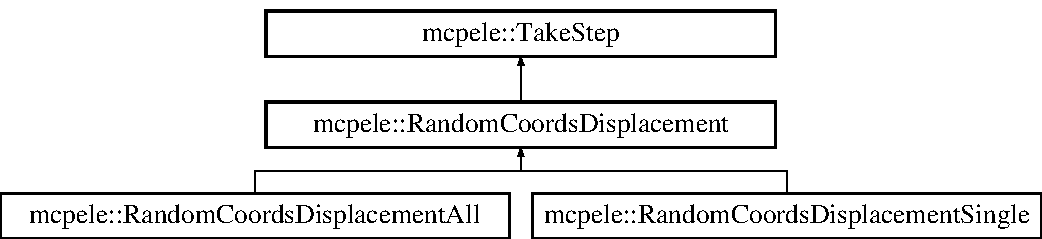
\includegraphics[height=3.000000cm]{classmcpele_1_1RandomCoordsDisplacement}
\end{center}
\end{figure}
\subsection*{\-Public \-Member \-Functions}
\begin{DoxyCompactItemize}
\item 
\hyperlink{classmcpele_1_1RandomCoordsDisplacement_a70c32449d74f21634737ebd382ede3aa}{\-Random\-Coords\-Displacement} (const size\-\_\-t rseed, const double stepsize=1)
\item 
virtual \hyperlink{classmcpele_1_1RandomCoordsDisplacement_a4603750d055490114b68f18b564e9fd4}{$\sim$\-Random\-Coords\-Displacement} ()
\item 
virtual void \hyperlink{classmcpele_1_1RandomCoordsDisplacement_aa6c2c40b2a36dc1711c5a7bbeeced708}{displace} (pele\-::\-Array$<$ double $>$ \&coords, \hyperlink{classmcpele_1_1MC}{\-M\-C} $\ast$mc)=0
\item 
size\-\_\-t \hyperlink{classmcpele_1_1RandomCoordsDisplacement_ac909159a4d7007b09cf5291af3415d82}{get\-\_\-seed} () const 
\item 
void \hyperlink{classmcpele_1_1RandomCoordsDisplacement_aaf9325c782ecb904a71e92671c7732fb}{set\-\_\-generator\-\_\-seed} (const size\-\_\-t inp)
\item 
double \hyperlink{classmcpele_1_1RandomCoordsDisplacement_ae8cff94bafe19a4fb529e2dbc8ac3ab1}{expected\-\_\-mean} () const 
\item 
double \hyperlink{classmcpele_1_1RandomCoordsDisplacement_a41cda87cd1b61178bc5035f9c4bcf753}{get\-\_\-stepsize} () const 
\item 
double \hyperlink{classmcpele_1_1RandomCoordsDisplacement_a77a73851c26beb001c8a48be76362a15}{expected\-\_\-variance} (const double ss) const 
\item 
void \hyperlink{classmcpele_1_1RandomCoordsDisplacement_abb8bd83d44eb248599c799f6ff76656f}{increase\-\_\-acceptance} (const double factor)
\item 
void \hyperlink{classmcpele_1_1RandomCoordsDisplacement_a75b39857737f466cee1ff4fe452d848e}{decrease\-\_\-acceptance} (const double factor)
\item 
size\-\_\-t \hyperlink{classmcpele_1_1RandomCoordsDisplacement_a37d0b36e6f3ec26e0ce3a5b5a381d661}{get\-\_\-count} () const 
\end{DoxyCompactItemize}
\subsection*{\-Protected \-Attributes}
\begin{DoxyCompactItemize}
\item 
size\-\_\-t \hyperlink{classmcpele_1_1RandomCoordsDisplacement_a1b60fa629821ec194d0d153716d26f73}{m\-\_\-seed}
\item 
std\-::mt19937\-\_\-64 \hyperlink{classmcpele_1_1RandomCoordsDisplacement_a6301d7fc89a1943a5fb7c870f25fe2a2}{m\-\_\-generator}
\item 
std\-::uniform\-\_\-real\-\_\-distribution\*
$<$ double $>$ \hyperlink{classmcpele_1_1RandomCoordsDisplacement_a8d3de3a3e1b9595baf9618bf1530c5e2}{m\-\_\-real\-\_\-distribution}
\item 
double \hyperlink{classmcpele_1_1RandomCoordsDisplacement_a523a1ff179209b62e574ebb3050f86a1}{m\-\_\-stepsize}
\item 
size\-\_\-t \hyperlink{classmcpele_1_1RandomCoordsDisplacement_aabfbc53faf2723b66852d634bb6f9b0a}{m\-\_\-count}
\end{DoxyCompactItemize}


\subsection{\-Detailed \-Description}
\-Random coords displacement, generates a random displacement for a \-N dimensional system sampling from a \-N-\/dimensional sphere. \-The stepsize is defined per coordinates, that's why the maximum stepsize is sqrt(\-N) $\ast$ stepsize. 

\-Definition at line 16 of file random\-\_\-coords\-\_\-displacement.\-h.



\subsection{\-Constructor \& \-Destructor \-Documentation}
\hypertarget{classmcpele_1_1RandomCoordsDisplacement_a70c32449d74f21634737ebd382ede3aa}{\index{mcpele\-::\-Random\-Coords\-Displacement@{mcpele\-::\-Random\-Coords\-Displacement}!\-Random\-Coords\-Displacement@{\-Random\-Coords\-Displacement}}
\index{\-Random\-Coords\-Displacement@{\-Random\-Coords\-Displacement}!mcpele::RandomCoordsDisplacement@{mcpele\-::\-Random\-Coords\-Displacement}}
\subsubsection[{\-Random\-Coords\-Displacement}]{\setlength{\rightskip}{0pt plus 5cm}{\bf mcpele\-::\-Random\-Coords\-Displacement\-::\-Random\-Coords\-Displacement} (
\begin{DoxyParamCaption}
\item[{const size\-\_\-t}]{rseed, }
\item[{const double}]{stepsize = {\ttfamily 1}}
\end{DoxyParamCaption}
)}}\label{classmcpele_1_1RandomCoordsDisplacement_a70c32449d74f21634737ebd382ede3aa}


\-Definition at line 7 of file random\-\_\-coords\-\_\-displacement.\-cpp.

\hypertarget{classmcpele_1_1RandomCoordsDisplacement_a4603750d055490114b68f18b564e9fd4}{\index{mcpele\-::\-Random\-Coords\-Displacement@{mcpele\-::\-Random\-Coords\-Displacement}!$\sim$\-Random\-Coords\-Displacement@{$\sim$\-Random\-Coords\-Displacement}}
\index{$\sim$\-Random\-Coords\-Displacement@{$\sim$\-Random\-Coords\-Displacement}!mcpele::RandomCoordsDisplacement@{mcpele\-::\-Random\-Coords\-Displacement}}
\subsubsection[{$\sim$\-Random\-Coords\-Displacement}]{\setlength{\rightskip}{0pt plus 5cm}virtual {\bf mcpele\-::\-Random\-Coords\-Displacement\-::$\sim$\-Random\-Coords\-Displacement} (
\begin{DoxyParamCaption}
{}
\end{DoxyParamCaption}
)\hspace{0.3cm}{\ttfamily  \mbox{[}inline, virtual\mbox{]}}}}\label{classmcpele_1_1RandomCoordsDisplacement_a4603750d055490114b68f18b564e9fd4}


\-Definition at line 25 of file random\-\_\-coords\-\_\-displacement.\-h.



\subsection{\-Member \-Function \-Documentation}
\hypertarget{classmcpele_1_1RandomCoordsDisplacement_a75b39857737f466cee1ff4fe452d848e}{\index{mcpele\-::\-Random\-Coords\-Displacement@{mcpele\-::\-Random\-Coords\-Displacement}!decrease\-\_\-acceptance@{decrease\-\_\-acceptance}}
\index{decrease\-\_\-acceptance@{decrease\-\_\-acceptance}!mcpele::RandomCoordsDisplacement@{mcpele\-::\-Random\-Coords\-Displacement}}
\subsubsection[{decrease\-\_\-acceptance}]{\setlength{\rightskip}{0pt plus 5cm}void {\bf mcpele\-::\-Random\-Coords\-Displacement\-::decrease\-\_\-acceptance} (
\begin{DoxyParamCaption}
\item[{const double}]{factor}
\end{DoxyParamCaption}
)\hspace{0.3cm}{\ttfamily  \mbox{[}inline, virtual\mbox{]}}}}\label{classmcpele_1_1RandomCoordsDisplacement_a75b39857737f466cee1ff4fe452d848e}


\-Reimplemented from \hyperlink{classmcpele_1_1TakeStep_a492ccf2a2e3b3d8ef2224947d0385d77}{mcpele\-::\-Take\-Step}.



\-Definition at line 36 of file random\-\_\-coords\-\_\-displacement.\-h.

\hypertarget{classmcpele_1_1RandomCoordsDisplacement_aa6c2c40b2a36dc1711c5a7bbeeced708}{\index{mcpele\-::\-Random\-Coords\-Displacement@{mcpele\-::\-Random\-Coords\-Displacement}!displace@{displace}}
\index{displace@{displace}!mcpele::RandomCoordsDisplacement@{mcpele\-::\-Random\-Coords\-Displacement}}
\subsubsection[{displace}]{\setlength{\rightskip}{0pt plus 5cm}virtual void {\bf mcpele\-::\-Random\-Coords\-Displacement\-::displace} (
\begin{DoxyParamCaption}
\item[{pele\-::\-Array$<$ double $>$ \&}]{coords, }
\item[{{\bf \-M\-C} $\ast$}]{mc}
\end{DoxyParamCaption}
)\hspace{0.3cm}{\ttfamily  \mbox{[}pure virtual\mbox{]}}}}\label{classmcpele_1_1RandomCoordsDisplacement_aa6c2c40b2a36dc1711c5a7bbeeced708}


\-Implements \hyperlink{classmcpele_1_1TakeStep_ac3032e0d99d4aa5f940ffea4a28442f5}{mcpele\-::\-Take\-Step}.



\-Implemented in \hyperlink{classmcpele_1_1RandomCoordsDisplacementSingle_a52c3271d105453d89024230f3f392dc7}{mcpele\-::\-Random\-Coords\-Displacement\-Single}, and \hyperlink{classmcpele_1_1RandomCoordsDisplacementAll_ab40ce59b2d74ffe3d8042c3e90268eab}{mcpele\-::\-Random\-Coords\-Displacement\-All}.

\hypertarget{classmcpele_1_1RandomCoordsDisplacement_ae8cff94bafe19a4fb529e2dbc8ac3ab1}{\index{mcpele\-::\-Random\-Coords\-Displacement@{mcpele\-::\-Random\-Coords\-Displacement}!expected\-\_\-mean@{expected\-\_\-mean}}
\index{expected\-\_\-mean@{expected\-\_\-mean}!mcpele::RandomCoordsDisplacement@{mcpele\-::\-Random\-Coords\-Displacement}}
\subsubsection[{expected\-\_\-mean}]{\setlength{\rightskip}{0pt plus 5cm}double {\bf mcpele\-::\-Random\-Coords\-Displacement\-::expected\-\_\-mean} (
\begin{DoxyParamCaption}
{}
\end{DoxyParamCaption}
) const\hspace{0.3cm}{\ttfamily  \mbox{[}inline\mbox{]}}}}\label{classmcpele_1_1RandomCoordsDisplacement_ae8cff94bafe19a4fb529e2dbc8ac3ab1}


\-Definition at line 29 of file random\-\_\-coords\-\_\-displacement.\-h.

\hypertarget{classmcpele_1_1RandomCoordsDisplacement_a77a73851c26beb001c8a48be76362a15}{\index{mcpele\-::\-Random\-Coords\-Displacement@{mcpele\-::\-Random\-Coords\-Displacement}!expected\-\_\-variance@{expected\-\_\-variance}}
\index{expected\-\_\-variance@{expected\-\_\-variance}!mcpele::RandomCoordsDisplacement@{mcpele\-::\-Random\-Coords\-Displacement}}
\subsubsection[{expected\-\_\-variance}]{\setlength{\rightskip}{0pt plus 5cm}double {\bf mcpele\-::\-Random\-Coords\-Displacement\-::expected\-\_\-variance} (
\begin{DoxyParamCaption}
\item[{const double}]{ss}
\end{DoxyParamCaption}
) const\hspace{0.3cm}{\ttfamily  \mbox{[}inline\mbox{]}}}}\label{classmcpele_1_1RandomCoordsDisplacement_a77a73851c26beb001c8a48be76362a15}
\-Reference\-: \href{http://mathworld.wolfram.com/UniformDistribution.html}{\tt http\-://mathworld.\-wolfram.\-com/\-Uniform\-Distribution.\-html} 

\-Definition at line 34 of file random\-\_\-coords\-\_\-displacement.\-h.

\hypertarget{classmcpele_1_1RandomCoordsDisplacement_a37d0b36e6f3ec26e0ce3a5b5a381d661}{\index{mcpele\-::\-Random\-Coords\-Displacement@{mcpele\-::\-Random\-Coords\-Displacement}!get\-\_\-count@{get\-\_\-count}}
\index{get\-\_\-count@{get\-\_\-count}!mcpele::RandomCoordsDisplacement@{mcpele\-::\-Random\-Coords\-Displacement}}
\subsubsection[{get\-\_\-count}]{\setlength{\rightskip}{0pt plus 5cm}size\-\_\-t {\bf mcpele\-::\-Random\-Coords\-Displacement\-::get\-\_\-count} (
\begin{DoxyParamCaption}
{}
\end{DoxyParamCaption}
) const\hspace{0.3cm}{\ttfamily  \mbox{[}inline\mbox{]}}}}\label{classmcpele_1_1RandomCoordsDisplacement_a37d0b36e6f3ec26e0ce3a5b5a381d661}


\-Definition at line 37 of file random\-\_\-coords\-\_\-displacement.\-h.

\hypertarget{classmcpele_1_1RandomCoordsDisplacement_ac909159a4d7007b09cf5291af3415d82}{\index{mcpele\-::\-Random\-Coords\-Displacement@{mcpele\-::\-Random\-Coords\-Displacement}!get\-\_\-seed@{get\-\_\-seed}}
\index{get\-\_\-seed@{get\-\_\-seed}!mcpele::RandomCoordsDisplacement@{mcpele\-::\-Random\-Coords\-Displacement}}
\subsubsection[{get\-\_\-seed}]{\setlength{\rightskip}{0pt plus 5cm}size\-\_\-t {\bf mcpele\-::\-Random\-Coords\-Displacement\-::get\-\_\-seed} (
\begin{DoxyParamCaption}
{}
\end{DoxyParamCaption}
) const\hspace{0.3cm}{\ttfamily  \mbox{[}inline\mbox{]}}}}\label{classmcpele_1_1RandomCoordsDisplacement_ac909159a4d7007b09cf5291af3415d82}


\-Definition at line 27 of file random\-\_\-coords\-\_\-displacement.\-h.

\hypertarget{classmcpele_1_1RandomCoordsDisplacement_a41cda87cd1b61178bc5035f9c4bcf753}{\index{mcpele\-::\-Random\-Coords\-Displacement@{mcpele\-::\-Random\-Coords\-Displacement}!get\-\_\-stepsize@{get\-\_\-stepsize}}
\index{get\-\_\-stepsize@{get\-\_\-stepsize}!mcpele::RandomCoordsDisplacement@{mcpele\-::\-Random\-Coords\-Displacement}}
\subsubsection[{get\-\_\-stepsize}]{\setlength{\rightskip}{0pt plus 5cm}double {\bf mcpele\-::\-Random\-Coords\-Displacement\-::get\-\_\-stepsize} (
\begin{DoxyParamCaption}
{}
\end{DoxyParamCaption}
) const\hspace{0.3cm}{\ttfamily  \mbox{[}inline\mbox{]}}}}\label{classmcpele_1_1RandomCoordsDisplacement_a41cda87cd1b61178bc5035f9c4bcf753}


\-Definition at line 30 of file random\-\_\-coords\-\_\-displacement.\-h.

\hypertarget{classmcpele_1_1RandomCoordsDisplacement_abb8bd83d44eb248599c799f6ff76656f}{\index{mcpele\-::\-Random\-Coords\-Displacement@{mcpele\-::\-Random\-Coords\-Displacement}!increase\-\_\-acceptance@{increase\-\_\-acceptance}}
\index{increase\-\_\-acceptance@{increase\-\_\-acceptance}!mcpele::RandomCoordsDisplacement@{mcpele\-::\-Random\-Coords\-Displacement}}
\subsubsection[{increase\-\_\-acceptance}]{\setlength{\rightskip}{0pt plus 5cm}void {\bf mcpele\-::\-Random\-Coords\-Displacement\-::increase\-\_\-acceptance} (
\begin{DoxyParamCaption}
\item[{const double}]{factor}
\end{DoxyParamCaption}
)\hspace{0.3cm}{\ttfamily  \mbox{[}inline, virtual\mbox{]}}}}\label{classmcpele_1_1RandomCoordsDisplacement_abb8bd83d44eb248599c799f6ff76656f}


\-Reimplemented from \hyperlink{classmcpele_1_1TakeStep_afa92f5196e0304d6ad910304b188c705}{mcpele\-::\-Take\-Step}.



\-Definition at line 35 of file random\-\_\-coords\-\_\-displacement.\-h.

\hypertarget{classmcpele_1_1RandomCoordsDisplacement_aaf9325c782ecb904a71e92671c7732fb}{\index{mcpele\-::\-Random\-Coords\-Displacement@{mcpele\-::\-Random\-Coords\-Displacement}!set\-\_\-generator\-\_\-seed@{set\-\_\-generator\-\_\-seed}}
\index{set\-\_\-generator\-\_\-seed@{set\-\_\-generator\-\_\-seed}!mcpele::RandomCoordsDisplacement@{mcpele\-::\-Random\-Coords\-Displacement}}
\subsubsection[{set\-\_\-generator\-\_\-seed}]{\setlength{\rightskip}{0pt plus 5cm}void {\bf mcpele\-::\-Random\-Coords\-Displacement\-::set\-\_\-generator\-\_\-seed} (
\begin{DoxyParamCaption}
\item[{const size\-\_\-t}]{inp}
\end{DoxyParamCaption}
)\hspace{0.3cm}{\ttfamily  \mbox{[}inline\mbox{]}}}}\label{classmcpele_1_1RandomCoordsDisplacement_aaf9325c782ecb904a71e92671c7732fb}


\-Definition at line 28 of file random\-\_\-coords\-\_\-displacement.\-h.



\subsection{\-Member \-Data \-Documentation}
\hypertarget{classmcpele_1_1RandomCoordsDisplacement_aabfbc53faf2723b66852d634bb6f9b0a}{\index{mcpele\-::\-Random\-Coords\-Displacement@{mcpele\-::\-Random\-Coords\-Displacement}!m\-\_\-count@{m\-\_\-count}}
\index{m\-\_\-count@{m\-\_\-count}!mcpele::RandomCoordsDisplacement@{mcpele\-::\-Random\-Coords\-Displacement}}
\subsubsection[{m\-\_\-count}]{\setlength{\rightskip}{0pt plus 5cm}size\-\_\-t {\bf mcpele\-::\-Random\-Coords\-Displacement\-::m\-\_\-count}\hspace{0.3cm}{\ttfamily  \mbox{[}protected\mbox{]}}}}\label{classmcpele_1_1RandomCoordsDisplacement_aabfbc53faf2723b66852d634bb6f9b0a}


\-Definition at line 22 of file random\-\_\-coords\-\_\-displacement.\-h.

\hypertarget{classmcpele_1_1RandomCoordsDisplacement_a6301d7fc89a1943a5fb7c870f25fe2a2}{\index{mcpele\-::\-Random\-Coords\-Displacement@{mcpele\-::\-Random\-Coords\-Displacement}!m\-\_\-generator@{m\-\_\-generator}}
\index{m\-\_\-generator@{m\-\_\-generator}!mcpele::RandomCoordsDisplacement@{mcpele\-::\-Random\-Coords\-Displacement}}
\subsubsection[{m\-\_\-generator}]{\setlength{\rightskip}{0pt plus 5cm}std\-::mt19937\-\_\-64 {\bf mcpele\-::\-Random\-Coords\-Displacement\-::m\-\_\-generator}\hspace{0.3cm}{\ttfamily  \mbox{[}protected\mbox{]}}}}\label{classmcpele_1_1RandomCoordsDisplacement_a6301d7fc89a1943a5fb7c870f25fe2a2}


\-Definition at line 19 of file random\-\_\-coords\-\_\-displacement.\-h.

\hypertarget{classmcpele_1_1RandomCoordsDisplacement_a8d3de3a3e1b9595baf9618bf1530c5e2}{\index{mcpele\-::\-Random\-Coords\-Displacement@{mcpele\-::\-Random\-Coords\-Displacement}!m\-\_\-real\-\_\-distribution@{m\-\_\-real\-\_\-distribution}}
\index{m\-\_\-real\-\_\-distribution@{m\-\_\-real\-\_\-distribution}!mcpele::RandomCoordsDisplacement@{mcpele\-::\-Random\-Coords\-Displacement}}
\subsubsection[{m\-\_\-real\-\_\-distribution}]{\setlength{\rightskip}{0pt plus 5cm}std\-::uniform\-\_\-real\-\_\-distribution$<$double$>$ {\bf mcpele\-::\-Random\-Coords\-Displacement\-::m\-\_\-real\-\_\-distribution}\hspace{0.3cm}{\ttfamily  \mbox{[}protected\mbox{]}}}}\label{classmcpele_1_1RandomCoordsDisplacement_a8d3de3a3e1b9595baf9618bf1530c5e2}


\-Definition at line 20 of file random\-\_\-coords\-\_\-displacement.\-h.

\hypertarget{classmcpele_1_1RandomCoordsDisplacement_a1b60fa629821ec194d0d153716d26f73}{\index{mcpele\-::\-Random\-Coords\-Displacement@{mcpele\-::\-Random\-Coords\-Displacement}!m\-\_\-seed@{m\-\_\-seed}}
\index{m\-\_\-seed@{m\-\_\-seed}!mcpele::RandomCoordsDisplacement@{mcpele\-::\-Random\-Coords\-Displacement}}
\subsubsection[{m\-\_\-seed}]{\setlength{\rightskip}{0pt plus 5cm}size\-\_\-t {\bf mcpele\-::\-Random\-Coords\-Displacement\-::m\-\_\-seed}\hspace{0.3cm}{\ttfamily  \mbox{[}protected\mbox{]}}}}\label{classmcpele_1_1RandomCoordsDisplacement_a1b60fa629821ec194d0d153716d26f73}


\-Definition at line 18 of file random\-\_\-coords\-\_\-displacement.\-h.

\hypertarget{classmcpele_1_1RandomCoordsDisplacement_a523a1ff179209b62e574ebb3050f86a1}{\index{mcpele\-::\-Random\-Coords\-Displacement@{mcpele\-::\-Random\-Coords\-Displacement}!m\-\_\-stepsize@{m\-\_\-stepsize}}
\index{m\-\_\-stepsize@{m\-\_\-stepsize}!mcpele::RandomCoordsDisplacement@{mcpele\-::\-Random\-Coords\-Displacement}}
\subsubsection[{m\-\_\-stepsize}]{\setlength{\rightskip}{0pt plus 5cm}double {\bf mcpele\-::\-Random\-Coords\-Displacement\-::m\-\_\-stepsize}\hspace{0.3cm}{\ttfamily  \mbox{[}protected\mbox{]}}}}\label{classmcpele_1_1RandomCoordsDisplacement_a523a1ff179209b62e574ebb3050f86a1}


\-Definition at line 21 of file random\-\_\-coords\-\_\-displacement.\-h.



\-The documentation for this class was generated from the following files\-:\begin{DoxyCompactItemize}
\item 
mcpele/\hyperlink{random__coords__displacement_8h}{random\-\_\-coords\-\_\-displacement.\-h}\item 
\hyperlink{random__coords__displacement_8cpp}{random\-\_\-coords\-\_\-displacement.\-cpp}\end{DoxyCompactItemize}

\hypertarget{classmcpele_1_1RandomCoordsDisplacementAll}{\section{mcpele\-:\-:\-Random\-Coords\-Displacement\-All \-Class \-Reference}
\label{classmcpele_1_1RandomCoordsDisplacementAll}\index{mcpele\-::\-Random\-Coords\-Displacement\-All@{mcpele\-::\-Random\-Coords\-Displacement\-All}}
}


{\ttfamily \#include $<$random\-\_\-coords\-\_\-displacement.\-h$>$}

\-Inheritance diagram for mcpele\-:\-:\-Random\-Coords\-Displacement\-All\-:\begin{figure}[H]
\begin{center}
\leavevmode
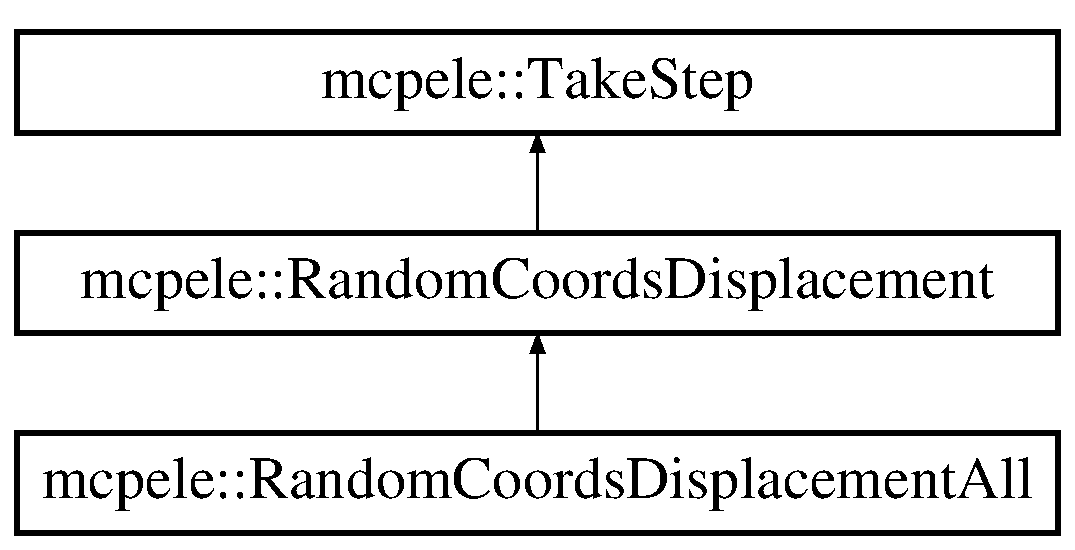
\includegraphics[height=3.000000cm]{classmcpele_1_1RandomCoordsDisplacementAll}
\end{center}
\end{figure}
\subsection*{\-Public \-Member \-Functions}
\begin{DoxyCompactItemize}
\item 
\hyperlink{classmcpele_1_1RandomCoordsDisplacementAll_aeddd85475bfd9fc2b0877259ce0fa6c8}{\-Random\-Coords\-Displacement\-All} (const size\-\_\-t rseed, const double stepsize=1)
\item 
virtual \hyperlink{classmcpele_1_1RandomCoordsDisplacementAll_ac80a8e168ea9f6e1f17d6462ce325492}{$\sim$\-Random\-Coords\-Displacement\-All} ()
\item 
virtual void \hyperlink{classmcpele_1_1RandomCoordsDisplacementAll_ab40ce59b2d74ffe3d8042c3e90268eab}{displace} (pele\-::\-Array$<$ double $>$ \&coords, \hyperlink{classmcpele_1_1MC}{\-M\-C} $\ast$mc)
\end{DoxyCompactItemize}


\subsection{\-Detailed \-Description}


\-Definition at line 40 of file random\-\_\-coords\-\_\-displacement.\-h.



\subsection{\-Constructor \& \-Destructor \-Documentation}
\hypertarget{classmcpele_1_1RandomCoordsDisplacementAll_aeddd85475bfd9fc2b0877259ce0fa6c8}{\index{mcpele\-::\-Random\-Coords\-Displacement\-All@{mcpele\-::\-Random\-Coords\-Displacement\-All}!\-Random\-Coords\-Displacement\-All@{\-Random\-Coords\-Displacement\-All}}
\index{\-Random\-Coords\-Displacement\-All@{\-Random\-Coords\-Displacement\-All}!mcpele::RandomCoordsDisplacementAll@{mcpele\-::\-Random\-Coords\-Displacement\-All}}
\subsubsection[{\-Random\-Coords\-Displacement\-All}]{\setlength{\rightskip}{0pt plus 5cm}{\bf mcpele\-::\-Random\-Coords\-Displacement\-All\-::\-Random\-Coords\-Displacement\-All} (
\begin{DoxyParamCaption}
\item[{const size\-\_\-t}]{rseed, }
\item[{const double}]{stepsize = {\ttfamily 1}}
\end{DoxyParamCaption}
)}}\label{classmcpele_1_1RandomCoordsDisplacementAll_aeddd85475bfd9fc2b0877259ce0fa6c8}


\-Definition at line 21 of file random\-\_\-coords\-\_\-displacement.\-cpp.

\hypertarget{classmcpele_1_1RandomCoordsDisplacementAll_ac80a8e168ea9f6e1f17d6462ce325492}{\index{mcpele\-::\-Random\-Coords\-Displacement\-All@{mcpele\-::\-Random\-Coords\-Displacement\-All}!$\sim$\-Random\-Coords\-Displacement\-All@{$\sim$\-Random\-Coords\-Displacement\-All}}
\index{$\sim$\-Random\-Coords\-Displacement\-All@{$\sim$\-Random\-Coords\-Displacement\-All}!mcpele::RandomCoordsDisplacementAll@{mcpele\-::\-Random\-Coords\-Displacement\-All}}
\subsubsection[{$\sim$\-Random\-Coords\-Displacement\-All}]{\setlength{\rightskip}{0pt plus 5cm}virtual {\bf mcpele\-::\-Random\-Coords\-Displacement\-All\-::$\sim$\-Random\-Coords\-Displacement\-All} (
\begin{DoxyParamCaption}
{}
\end{DoxyParamCaption}
)\hspace{0.3cm}{\ttfamily  \mbox{[}inline, virtual\mbox{]}}}}\label{classmcpele_1_1RandomCoordsDisplacementAll_ac80a8e168ea9f6e1f17d6462ce325492}


\-Definition at line 43 of file random\-\_\-coords\-\_\-displacement.\-h.



\subsection{\-Member \-Function \-Documentation}
\hypertarget{classmcpele_1_1RandomCoordsDisplacementAll_ab40ce59b2d74ffe3d8042c3e90268eab}{\index{mcpele\-::\-Random\-Coords\-Displacement\-All@{mcpele\-::\-Random\-Coords\-Displacement\-All}!displace@{displace}}
\index{displace@{displace}!mcpele::RandomCoordsDisplacementAll@{mcpele\-::\-Random\-Coords\-Displacement\-All}}
\subsubsection[{displace}]{\setlength{\rightskip}{0pt plus 5cm}void {\bf mcpele\-::\-Random\-Coords\-Displacement\-All\-::displace} (
\begin{DoxyParamCaption}
\item[{pele\-::\-Array$<$ double $>$ \&}]{coords, }
\item[{{\bf \-M\-C} $\ast$}]{mc}
\end{DoxyParamCaption}
)\hspace{0.3cm}{\ttfamily  \mbox{[}virtual\mbox{]}}}}\label{classmcpele_1_1RandomCoordsDisplacementAll_ab40ce59b2d74ffe3d8042c3e90268eab}


\-Implements \hyperlink{classmcpele_1_1RandomCoordsDisplacement_aa6c2c40b2a36dc1711c5a7bbeeced708}{mcpele\-::\-Random\-Coords\-Displacement}.



\-Definition at line 24 of file random\-\_\-coords\-\_\-displacement.\-cpp.



\-The documentation for this class was generated from the following files\-:\begin{DoxyCompactItemize}
\item 
mcpele/\hyperlink{random__coords__displacement_8h}{random\-\_\-coords\-\_\-displacement.\-h}\item 
\hyperlink{random__coords__displacement_8cpp}{random\-\_\-coords\-\_\-displacement.\-cpp}\end{DoxyCompactItemize}

\hypertarget{classmcpele_1_1RandomCoordsDisplacementSingle}{\section{mcpele\-:\-:\-Random\-Coords\-Displacement\-Single \-Class \-Reference}
\label{classmcpele_1_1RandomCoordsDisplacementSingle}\index{mcpele\-::\-Random\-Coords\-Displacement\-Single@{mcpele\-::\-Random\-Coords\-Displacement\-Single}}
}


{\ttfamily \#include $<$random\-\_\-coords\-\_\-displacement.\-h$>$}

\-Inheritance diagram for mcpele\-:\-:\-Random\-Coords\-Displacement\-Single\-:\begin{figure}[H]
\begin{center}
\leavevmode
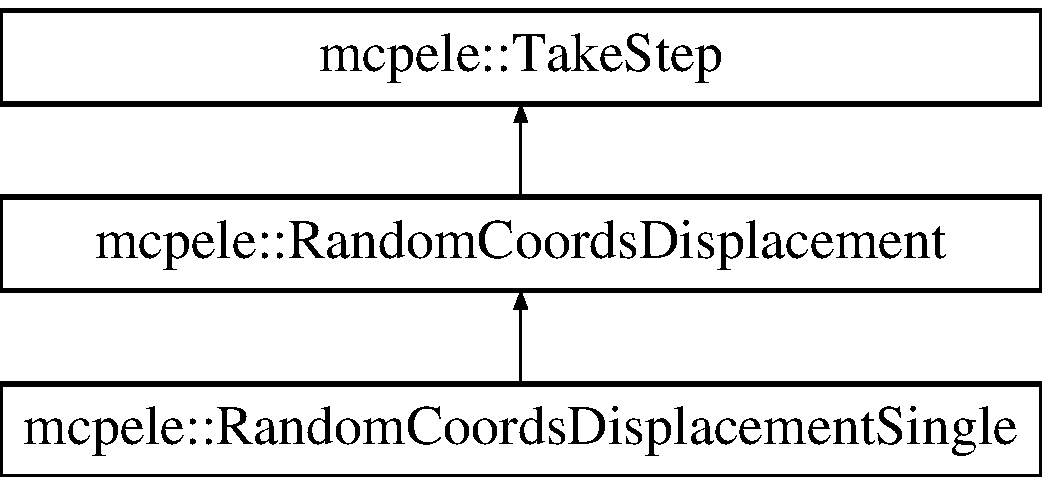
\includegraphics[height=3.000000cm]{classmcpele_1_1RandomCoordsDisplacementSingle}
\end{center}
\end{figure}
\subsection*{\-Public \-Member \-Functions}
\begin{DoxyCompactItemize}
\item 
\hyperlink{classmcpele_1_1RandomCoordsDisplacementSingle_a5a5ff549e6129c94d87bf4416f23574f}{\-Random\-Coords\-Displacement\-Single} (const size\-\_\-t rseed, const size\-\_\-t nparticles, const size\-\_\-t ndim, const double stepsize=1)
\item 
virtual \hyperlink{classmcpele_1_1RandomCoordsDisplacementSingle_a96c89a89af34b00f2705cd226e94142d}{$\sim$\-Random\-Coords\-Displacement\-Single} ()
\item 
virtual void \hyperlink{classmcpele_1_1RandomCoordsDisplacementSingle_a52c3271d105453d89024230f3f392dc7}{displace} (pele\-::\-Array$<$ double $>$ \&coords, \hyperlink{classmcpele_1_1MC}{\-M\-C} $\ast$mc)
\item 
size\-\_\-t \hyperlink{classmcpele_1_1RandomCoordsDisplacementSingle_a86f20835fae2527099165f24e894788b}{get\-\_\-rand\-\_\-particle} ()
\end{DoxyCompactItemize}


\subsection{\-Detailed \-Description}


\-Definition at line 47 of file random\-\_\-coords\-\_\-displacement.\-h.



\subsection{\-Constructor \& \-Destructor \-Documentation}
\hypertarget{classmcpele_1_1RandomCoordsDisplacementSingle_a5a5ff549e6129c94d87bf4416f23574f}{\index{mcpele\-::\-Random\-Coords\-Displacement\-Single@{mcpele\-::\-Random\-Coords\-Displacement\-Single}!\-Random\-Coords\-Displacement\-Single@{\-Random\-Coords\-Displacement\-Single}}
\index{\-Random\-Coords\-Displacement\-Single@{\-Random\-Coords\-Displacement\-Single}!mcpele::RandomCoordsDisplacementSingle@{mcpele\-::\-Random\-Coords\-Displacement\-Single}}
\subsubsection[{\-Random\-Coords\-Displacement\-Single}]{\setlength{\rightskip}{0pt plus 5cm}{\bf mcpele\-::\-Random\-Coords\-Displacement\-Single\-::\-Random\-Coords\-Displacement\-Single} (
\begin{DoxyParamCaption}
\item[{const size\-\_\-t}]{rseed, }
\item[{const size\-\_\-t}]{nparticles, }
\item[{const size\-\_\-t}]{ndim, }
\item[{const double}]{stepsize = {\ttfamily 1}}
\end{DoxyParamCaption}
)}}\label{classmcpele_1_1RandomCoordsDisplacementSingle_a5a5ff549e6129c94d87bf4416f23574f}


\-Definition at line 35 of file random\-\_\-coords\-\_\-displacement.\-cpp.

\hypertarget{classmcpele_1_1RandomCoordsDisplacementSingle_a96c89a89af34b00f2705cd226e94142d}{\index{mcpele\-::\-Random\-Coords\-Displacement\-Single@{mcpele\-::\-Random\-Coords\-Displacement\-Single}!$\sim$\-Random\-Coords\-Displacement\-Single@{$\sim$\-Random\-Coords\-Displacement\-Single}}
\index{$\sim$\-Random\-Coords\-Displacement\-Single@{$\sim$\-Random\-Coords\-Displacement\-Single}!mcpele::RandomCoordsDisplacementSingle@{mcpele\-::\-Random\-Coords\-Displacement\-Single}}
\subsubsection[{$\sim$\-Random\-Coords\-Displacement\-Single}]{\setlength{\rightskip}{0pt plus 5cm}virtual {\bf mcpele\-::\-Random\-Coords\-Displacement\-Single\-::$\sim$\-Random\-Coords\-Displacement\-Single} (
\begin{DoxyParamCaption}
{}
\end{DoxyParamCaption}
)\hspace{0.3cm}{\ttfamily  \mbox{[}inline, virtual\mbox{]}}}}\label{classmcpele_1_1RandomCoordsDisplacementSingle_a96c89a89af34b00f2705cd226e94142d}


\-Definition at line 52 of file random\-\_\-coords\-\_\-displacement.\-h.



\subsection{\-Member \-Function \-Documentation}
\hypertarget{classmcpele_1_1RandomCoordsDisplacementSingle_a52c3271d105453d89024230f3f392dc7}{\index{mcpele\-::\-Random\-Coords\-Displacement\-Single@{mcpele\-::\-Random\-Coords\-Displacement\-Single}!displace@{displace}}
\index{displace@{displace}!mcpele::RandomCoordsDisplacementSingle@{mcpele\-::\-Random\-Coords\-Displacement\-Single}}
\subsubsection[{displace}]{\setlength{\rightskip}{0pt plus 5cm}void {\bf mcpele\-::\-Random\-Coords\-Displacement\-Single\-::displace} (
\begin{DoxyParamCaption}
\item[{pele\-::\-Array$<$ double $>$ \&}]{coords, }
\item[{{\bf \-M\-C} $\ast$}]{mc}
\end{DoxyParamCaption}
)\hspace{0.3cm}{\ttfamily  \mbox{[}virtual\mbox{]}}}}\label{classmcpele_1_1RandomCoordsDisplacementSingle_a52c3271d105453d89024230f3f392dc7}


\-Implements \hyperlink{classmcpele_1_1RandomCoordsDisplacement_aa6c2c40b2a36dc1711c5a7bbeeced708}{mcpele\-::\-Random\-Coords\-Displacement}.



\-Definition at line 42 of file random\-\_\-coords\-\_\-displacement.\-cpp.

\hypertarget{classmcpele_1_1RandomCoordsDisplacementSingle_a86f20835fae2527099165f24e894788b}{\index{mcpele\-::\-Random\-Coords\-Displacement\-Single@{mcpele\-::\-Random\-Coords\-Displacement\-Single}!get\-\_\-rand\-\_\-particle@{get\-\_\-rand\-\_\-particle}}
\index{get\-\_\-rand\-\_\-particle@{get\-\_\-rand\-\_\-particle}!mcpele::RandomCoordsDisplacementSingle@{mcpele\-::\-Random\-Coords\-Displacement\-Single}}
\subsubsection[{get\-\_\-rand\-\_\-particle}]{\setlength{\rightskip}{0pt plus 5cm}size\-\_\-t {\bf mcpele\-::\-Random\-Coords\-Displacement\-Single\-::get\-\_\-rand\-\_\-particle} (
\begin{DoxyParamCaption}
{}
\end{DoxyParamCaption}
)\hspace{0.3cm}{\ttfamily  \mbox{[}inline\mbox{]}}}}\label{classmcpele_1_1RandomCoordsDisplacementSingle_a86f20835fae2527099165f24e894788b}


\-Definition at line 54 of file random\-\_\-coords\-\_\-displacement.\-h.



\-The documentation for this class was generated from the following files\-:\begin{DoxyCompactItemize}
\item 
mcpele/\hyperlink{random__coords__displacement_8h}{random\-\_\-coords\-\_\-displacement.\-h}\item 
\hyperlink{random__coords__displacement_8cpp}{random\-\_\-coords\-\_\-displacement.\-cpp}\end{DoxyCompactItemize}

\hypertarget{classmcpele_1_1RecordDisplacementPerParticleTimeseries}{\section{mcpele\-:\-:\-Record\-Displacement\-Per\-Particle\-Timeseries \-Class \-Reference}
\label{classmcpele_1_1RecordDisplacementPerParticleTimeseries}\index{mcpele\-::\-Record\-Displacement\-Per\-Particle\-Timeseries@{mcpele\-::\-Record\-Displacement\-Per\-Particle\-Timeseries}}
}


{\ttfamily \#include $<$record\-\_\-displacement\-\_\-per\-\_\-particle\-\_\-timeseries.\-h$>$}

\-Inheritance diagram for mcpele\-:\-:\-Record\-Displacement\-Per\-Particle\-Timeseries\-:\begin{figure}[H]
\begin{center}
\leavevmode
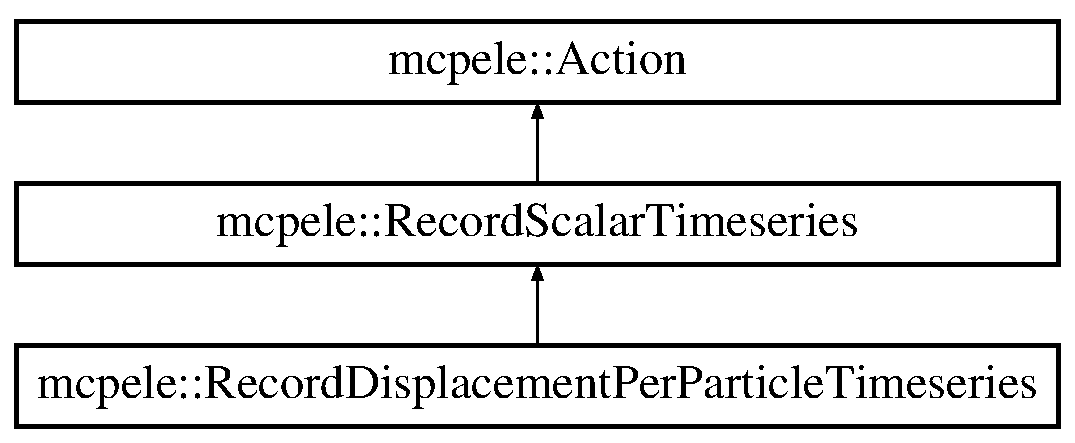
\includegraphics[height=3.000000cm]{classmcpele_1_1RecordDisplacementPerParticleTimeseries}
\end{center}
\end{figure}
\subsection*{\-Public \-Member \-Functions}
\begin{DoxyCompactItemize}
\item 
\hyperlink{classmcpele_1_1RecordDisplacementPerParticleTimeseries_a43afba63785193f65c9db66b040ed6d8}{\-Record\-Displacement\-Per\-Particle\-Timeseries} (const size\-\_\-t niter, const size\-\_\-t record\-\_\-every, pele\-::\-Array$<$ double $>$ initial\-\_\-coords, const size\-\_\-t boxdimension)
\item 
virtual \hyperlink{classmcpele_1_1RecordDisplacementPerParticleTimeseries_add341ebe1011d36c53df06ddc256fdbf}{$\sim$\-Record\-Displacement\-Per\-Particle\-Timeseries} ()
\item 
virtual double \hyperlink{classmcpele_1_1RecordDisplacementPerParticleTimeseries_ac049afa25de4847b76910680cb3f1a10}{get\-\_\-recorded\-\_\-scalar} (pele\-::\-Array$<$ double $>$ \&coords, const double energy, const bool accepted, \hyperlink{classmcpele_1_1MC}{\-M\-C} $\ast$mc)
\end{DoxyCompactItemize}


\subsection{\-Detailed \-Description}
\-Record time series of mean displacement per particle. \-Motivation\-: check if \-H\-S fluid is decorrelated between snapshots \-This is useful if particles are not placed back into periodic box. 

\-Definition at line 14 of file record\-\_\-displacement\-\_\-per\-\_\-particle\-\_\-timeseries.\-h.



\subsection{\-Constructor \& \-Destructor \-Documentation}
\hypertarget{classmcpele_1_1RecordDisplacementPerParticleTimeseries_a43afba63785193f65c9db66b040ed6d8}{\index{mcpele\-::\-Record\-Displacement\-Per\-Particle\-Timeseries@{mcpele\-::\-Record\-Displacement\-Per\-Particle\-Timeseries}!\-Record\-Displacement\-Per\-Particle\-Timeseries@{\-Record\-Displacement\-Per\-Particle\-Timeseries}}
\index{\-Record\-Displacement\-Per\-Particle\-Timeseries@{\-Record\-Displacement\-Per\-Particle\-Timeseries}!mcpele::RecordDisplacementPerParticleTimeseries@{mcpele\-::\-Record\-Displacement\-Per\-Particle\-Timeseries}}
\subsubsection[{\-Record\-Displacement\-Per\-Particle\-Timeseries}]{\setlength{\rightskip}{0pt plus 5cm}{\bf mcpele\-::\-Record\-Displacement\-Per\-Particle\-Timeseries\-::\-Record\-Displacement\-Per\-Particle\-Timeseries} (
\begin{DoxyParamCaption}
\item[{const size\-\_\-t}]{niter, }
\item[{const size\-\_\-t}]{record\-\_\-every, }
\item[{pele\-::\-Array$<$ double $>$}]{initial\-\_\-coords, }
\item[{const size\-\_\-t}]{boxdimension}
\end{DoxyParamCaption}
)\hspace{0.3cm}{\ttfamily  \mbox{[}inline\mbox{]}}}}\label{classmcpele_1_1RecordDisplacementPerParticleTimeseries_a43afba63785193f65c9db66b040ed6d8}


\-Definition at line 18 of file record\-\_\-displacement\-\_\-per\-\_\-particle\-\_\-timeseries.\-h.

\hypertarget{classmcpele_1_1RecordDisplacementPerParticleTimeseries_add341ebe1011d36c53df06ddc256fdbf}{\index{mcpele\-::\-Record\-Displacement\-Per\-Particle\-Timeseries@{mcpele\-::\-Record\-Displacement\-Per\-Particle\-Timeseries}!$\sim$\-Record\-Displacement\-Per\-Particle\-Timeseries@{$\sim$\-Record\-Displacement\-Per\-Particle\-Timeseries}}
\index{$\sim$\-Record\-Displacement\-Per\-Particle\-Timeseries@{$\sim$\-Record\-Displacement\-Per\-Particle\-Timeseries}!mcpele::RecordDisplacementPerParticleTimeseries@{mcpele\-::\-Record\-Displacement\-Per\-Particle\-Timeseries}}
\subsubsection[{$\sim$\-Record\-Displacement\-Per\-Particle\-Timeseries}]{\setlength{\rightskip}{0pt plus 5cm}virtual {\bf mcpele\-::\-Record\-Displacement\-Per\-Particle\-Timeseries\-::$\sim$\-Record\-Displacement\-Per\-Particle\-Timeseries} (
\begin{DoxyParamCaption}
{}
\end{DoxyParamCaption}
)\hspace{0.3cm}{\ttfamily  \mbox{[}inline, virtual\mbox{]}}}}\label{classmcpele_1_1RecordDisplacementPerParticleTimeseries_add341ebe1011d36c53df06ddc256fdbf}


\-Definition at line 24 of file record\-\_\-displacement\-\_\-per\-\_\-particle\-\_\-timeseries.\-h.



\subsection{\-Member \-Function \-Documentation}
\hypertarget{classmcpele_1_1RecordDisplacementPerParticleTimeseries_ac049afa25de4847b76910680cb3f1a10}{\index{mcpele\-::\-Record\-Displacement\-Per\-Particle\-Timeseries@{mcpele\-::\-Record\-Displacement\-Per\-Particle\-Timeseries}!get\-\_\-recorded\-\_\-scalar@{get\-\_\-recorded\-\_\-scalar}}
\index{get\-\_\-recorded\-\_\-scalar@{get\-\_\-recorded\-\_\-scalar}!mcpele::RecordDisplacementPerParticleTimeseries@{mcpele\-::\-Record\-Displacement\-Per\-Particle\-Timeseries}}
\subsubsection[{get\-\_\-recorded\-\_\-scalar}]{\setlength{\rightskip}{0pt plus 5cm}virtual double {\bf mcpele\-::\-Record\-Displacement\-Per\-Particle\-Timeseries\-::get\-\_\-recorded\-\_\-scalar} (
\begin{DoxyParamCaption}
\item[{pele\-::\-Array$<$ double $>$ \&}]{coords, }
\item[{const double}]{energy, }
\item[{const bool}]{accepted, }
\item[{{\bf \-M\-C} $\ast$}]{mc}
\end{DoxyParamCaption}
)\hspace{0.3cm}{\ttfamily  \mbox{[}inline, virtual\mbox{]}}}}\label{classmcpele_1_1RecordDisplacementPerParticleTimeseries_ac049afa25de4847b76910680cb3f1a10}


\-Implements \hyperlink{classmcpele_1_1RecordScalarTimeseries_a8151f9f679c926d481e7354ac170663a}{mcpele\-::\-Record\-Scalar\-Timeseries}.



\-Definition at line 25 of file record\-\_\-displacement\-\_\-per\-\_\-particle\-\_\-timeseries.\-h.



\-The documentation for this class was generated from the following file\-:\begin{DoxyCompactItemize}
\item 
mcpele/\hyperlink{record__displacement__per__particle__timeseries_8h}{record\-\_\-displacement\-\_\-per\-\_\-particle\-\_\-timeseries.\-h}\end{DoxyCompactItemize}

\hypertarget{classmcpele_1_1RecordEnergyHistogram}{\section{mcpele\-:\-:\-Record\-Energy\-Histogram \-Class \-Reference}
\label{classmcpele_1_1RecordEnergyHistogram}\index{mcpele\-::\-Record\-Energy\-Histogram@{mcpele\-::\-Record\-Energy\-Histogram}}
}


{\ttfamily \#include $<$record\-\_\-energy\-\_\-histogram.\-h$>$}

\-Inheritance diagram for mcpele\-:\-:\-Record\-Energy\-Histogram\-:\begin{figure}[H]
\begin{center}
\leavevmode
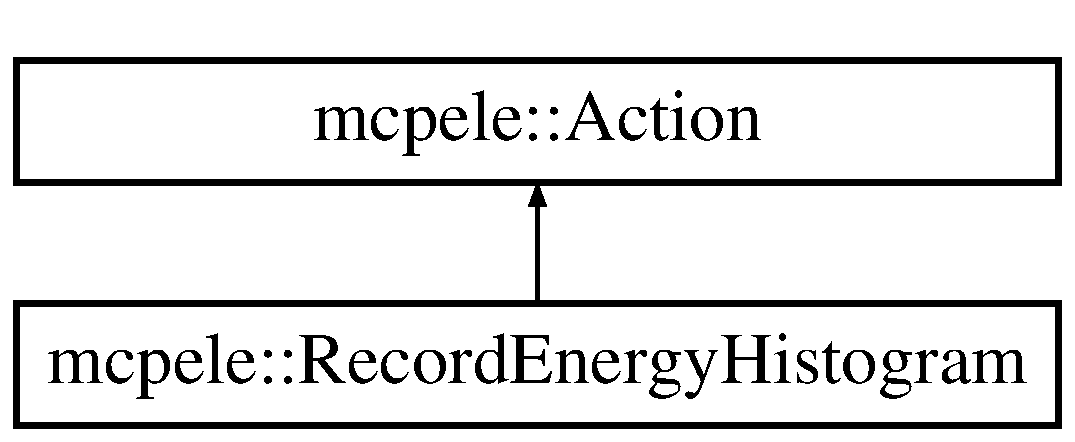
\includegraphics[height=2.000000cm]{classmcpele_1_1RecordEnergyHistogram}
\end{center}
\end{figure}
\subsection*{\-Public \-Member \-Functions}
\begin{DoxyCompactItemize}
\item 
\hyperlink{classmcpele_1_1RecordEnergyHistogram_a33f921c473b0e72b1965466d00951907}{\-Record\-Energy\-Histogram} (const double min, const double max, const double bin, const size\-\_\-t eqsteps)
\item 
virtual \hyperlink{classmcpele_1_1RecordEnergyHistogram_a4635539552b05ae80b711141783591d2}{$\sim$\-Record\-Energy\-Histogram} ()
\item 
virtual void \hyperlink{classmcpele_1_1RecordEnergyHistogram_af0aa711e4556dff5ae5837e42be17ecc}{action} (pele\-::\-Array$<$ double $>$ \&coords, double energy, bool accepted, \hyperlink{classmcpele_1_1MC}{\-M\-C} $\ast$mc)
\item 
pele\-::\-Array$<$ double $>$ \hyperlink{classmcpele_1_1RecordEnergyHistogram_a9e4df47ed681ca5de613bab6021bf32c}{get\-\_\-histogram} () const 
\item 
void \hyperlink{classmcpele_1_1RecordEnergyHistogram_adb151dfde34fbf2ea0317ee263d76c6b}{print\-\_\-terminal} () const 
\item 
double \hyperlink{classmcpele_1_1RecordEnergyHistogram_aab9cbcb6bfe0e402c225cb2d24c89d07}{get\-\_\-max} () const 
\item 
double \hyperlink{classmcpele_1_1RecordEnergyHistogram_abff6ed2dcf35f522d157401488402e42}{get\-\_\-min} () const 
\item 
size\-\_\-t \hyperlink{classmcpele_1_1RecordEnergyHistogram_acfe168ed7f14c8844acdb558c7dd1552}{get\-\_\-eqsteps} () const 
\item 
double \hyperlink{classmcpele_1_1RecordEnergyHistogram_a978c1bb832d0904664d108102e90abe2}{get\-\_\-mean} () const 
\item 
double \hyperlink{classmcpele_1_1RecordEnergyHistogram_a7246334bfba14e88b80cd4483b3e3eec}{get\-\_\-variance} () const 
\item 
int \hyperlink{classmcpele_1_1RecordEnergyHistogram_a551a641f1e019ba960d2feecd2ddabf0}{get\-\_\-entries} () const 
\end{DoxyCompactItemize}
\subsection*{\-Protected \-Attributes}
\begin{DoxyCompactItemize}
\item 
\hyperlink{classmcpele_1_1Histogram}{mcpele\-::\-Histogram} \hyperlink{classmcpele_1_1RecordEnergyHistogram_a5c6bc30e23e724736b75e7ed61b55ca1}{m\-\_\-hist}
\end{DoxyCompactItemize}


\subsection{\-Detailed \-Description}


\-Definition at line 13 of file record\-\_\-energy\-\_\-histogram.\-h.



\subsection{\-Constructor \& \-Destructor \-Documentation}
\hypertarget{classmcpele_1_1RecordEnergyHistogram_a33f921c473b0e72b1965466d00951907}{\index{mcpele\-::\-Record\-Energy\-Histogram@{mcpele\-::\-Record\-Energy\-Histogram}!\-Record\-Energy\-Histogram@{\-Record\-Energy\-Histogram}}
\index{\-Record\-Energy\-Histogram@{\-Record\-Energy\-Histogram}!mcpele::RecordEnergyHistogram@{mcpele\-::\-Record\-Energy\-Histogram}}
\subsubsection[{\-Record\-Energy\-Histogram}]{\setlength{\rightskip}{0pt plus 5cm}{\bf mcpele\-::\-Record\-Energy\-Histogram\-::\-Record\-Energy\-Histogram} (
\begin{DoxyParamCaption}
\item[{const double}]{min, }
\item[{const double}]{max, }
\item[{const double}]{bin, }
\item[{const size\-\_\-t}]{eqsteps}
\end{DoxyParamCaption}
)}}\label{classmcpele_1_1RecordEnergyHistogram_a33f921c473b0e72b1965466d00951907}


\-Definition at line 7 of file record\-\_\-energy\-\_\-histogram.\-cpp.

\hypertarget{classmcpele_1_1RecordEnergyHistogram_a4635539552b05ae80b711141783591d2}{\index{mcpele\-::\-Record\-Energy\-Histogram@{mcpele\-::\-Record\-Energy\-Histogram}!$\sim$\-Record\-Energy\-Histogram@{$\sim$\-Record\-Energy\-Histogram}}
\index{$\sim$\-Record\-Energy\-Histogram@{$\sim$\-Record\-Energy\-Histogram}!mcpele::RecordEnergyHistogram@{mcpele\-::\-Record\-Energy\-Histogram}}
\subsubsection[{$\sim$\-Record\-Energy\-Histogram}]{\setlength{\rightskip}{0pt plus 5cm}virtual {\bf mcpele\-::\-Record\-Energy\-Histogram\-::$\sim$\-Record\-Energy\-Histogram} (
\begin{DoxyParamCaption}
{}
\end{DoxyParamCaption}
)\hspace{0.3cm}{\ttfamily  \mbox{[}inline, virtual\mbox{]}}}}\label{classmcpele_1_1RecordEnergyHistogram_a4635539552b05ae80b711141783591d2}


\-Definition at line 21 of file record\-\_\-energy\-\_\-histogram.\-h.



\subsection{\-Member \-Function \-Documentation}
\hypertarget{classmcpele_1_1RecordEnergyHistogram_af0aa711e4556dff5ae5837e42be17ecc}{\index{mcpele\-::\-Record\-Energy\-Histogram@{mcpele\-::\-Record\-Energy\-Histogram}!action@{action}}
\index{action@{action}!mcpele::RecordEnergyHistogram@{mcpele\-::\-Record\-Energy\-Histogram}}
\subsubsection[{action}]{\setlength{\rightskip}{0pt plus 5cm}void {\bf mcpele\-::\-Record\-Energy\-Histogram\-::action} (
\begin{DoxyParamCaption}
\item[{pele\-::\-Array$<$ double $>$ \&}]{coords, }
\item[{double}]{energy, }
\item[{bool}]{accepted, }
\item[{{\bf \-M\-C} $\ast$}]{mc}
\end{DoxyParamCaption}
)\hspace{0.3cm}{\ttfamily  \mbox{[}virtual\mbox{]}}}}\label{classmcpele_1_1RecordEnergyHistogram_af0aa711e4556dff5ae5837e42be17ecc}


\-Implements \hyperlink{classmcpele_1_1Action_a9500d60c55f0d36ffb6ed0464ea3c68e}{mcpele\-::\-Action}.



\-Definition at line 13 of file record\-\_\-energy\-\_\-histogram.\-cpp.

\hypertarget{classmcpele_1_1RecordEnergyHistogram_a551a641f1e019ba960d2feecd2ddabf0}{\index{mcpele\-::\-Record\-Energy\-Histogram@{mcpele\-::\-Record\-Energy\-Histogram}!get\-\_\-entries@{get\-\_\-entries}}
\index{get\-\_\-entries@{get\-\_\-entries}!mcpele::RecordEnergyHistogram@{mcpele\-::\-Record\-Energy\-Histogram}}
\subsubsection[{get\-\_\-entries}]{\setlength{\rightskip}{0pt plus 5cm}int {\bf mcpele\-::\-Record\-Energy\-Histogram\-::get\-\_\-entries} (
\begin{DoxyParamCaption}
{}
\end{DoxyParamCaption}
) const\hspace{0.3cm}{\ttfamily  \mbox{[}inline\mbox{]}}}}\label{classmcpele_1_1RecordEnergyHistogram_a551a641f1e019ba960d2feecd2ddabf0}


\-Definition at line 30 of file record\-\_\-energy\-\_\-histogram.\-h.

\hypertarget{classmcpele_1_1RecordEnergyHistogram_acfe168ed7f14c8844acdb558c7dd1552}{\index{mcpele\-::\-Record\-Energy\-Histogram@{mcpele\-::\-Record\-Energy\-Histogram}!get\-\_\-eqsteps@{get\-\_\-eqsteps}}
\index{get\-\_\-eqsteps@{get\-\_\-eqsteps}!mcpele::RecordEnergyHistogram@{mcpele\-::\-Record\-Energy\-Histogram}}
\subsubsection[{get\-\_\-eqsteps}]{\setlength{\rightskip}{0pt plus 5cm}size\-\_\-t {\bf mcpele\-::\-Record\-Energy\-Histogram\-::get\-\_\-eqsteps} (
\begin{DoxyParamCaption}
{}
\end{DoxyParamCaption}
) const\hspace{0.3cm}{\ttfamily  \mbox{[}inline\mbox{]}}}}\label{classmcpele_1_1RecordEnergyHistogram_acfe168ed7f14c8844acdb558c7dd1552}


\-Definition at line 27 of file record\-\_\-energy\-\_\-histogram.\-h.

\hypertarget{classmcpele_1_1RecordEnergyHistogram_a9e4df47ed681ca5de613bab6021bf32c}{\index{mcpele\-::\-Record\-Energy\-Histogram@{mcpele\-::\-Record\-Energy\-Histogram}!get\-\_\-histogram@{get\-\_\-histogram}}
\index{get\-\_\-histogram@{get\-\_\-histogram}!mcpele::RecordEnergyHistogram@{mcpele\-::\-Record\-Energy\-Histogram}}
\subsubsection[{get\-\_\-histogram}]{\setlength{\rightskip}{0pt plus 5cm}pele\-::\-Array$<$ double $>$ {\bf mcpele\-::\-Record\-Energy\-Histogram\-::get\-\_\-histogram} (
\begin{DoxyParamCaption}
{}
\end{DoxyParamCaption}
) const}}\label{classmcpele_1_1RecordEnergyHistogram_a9e4df47ed681ca5de613bab6021bf32c}


\-Definition at line 21 of file record\-\_\-energy\-\_\-histogram.\-cpp.

\hypertarget{classmcpele_1_1RecordEnergyHistogram_aab9cbcb6bfe0e402c225cb2d24c89d07}{\index{mcpele\-::\-Record\-Energy\-Histogram@{mcpele\-::\-Record\-Energy\-Histogram}!get\-\_\-max@{get\-\_\-max}}
\index{get\-\_\-max@{get\-\_\-max}!mcpele::RecordEnergyHistogram@{mcpele\-::\-Record\-Energy\-Histogram}}
\subsubsection[{get\-\_\-max}]{\setlength{\rightskip}{0pt plus 5cm}double {\bf mcpele\-::\-Record\-Energy\-Histogram\-::get\-\_\-max} (
\begin{DoxyParamCaption}
{}
\end{DoxyParamCaption}
) const\hspace{0.3cm}{\ttfamily  \mbox{[}inline\mbox{]}}}}\label{classmcpele_1_1RecordEnergyHistogram_aab9cbcb6bfe0e402c225cb2d24c89d07}


\-Definition at line 25 of file record\-\_\-energy\-\_\-histogram.\-h.

\hypertarget{classmcpele_1_1RecordEnergyHistogram_a978c1bb832d0904664d108102e90abe2}{\index{mcpele\-::\-Record\-Energy\-Histogram@{mcpele\-::\-Record\-Energy\-Histogram}!get\-\_\-mean@{get\-\_\-mean}}
\index{get\-\_\-mean@{get\-\_\-mean}!mcpele::RecordEnergyHistogram@{mcpele\-::\-Record\-Energy\-Histogram}}
\subsubsection[{get\-\_\-mean}]{\setlength{\rightskip}{0pt plus 5cm}double {\bf mcpele\-::\-Record\-Energy\-Histogram\-::get\-\_\-mean} (
\begin{DoxyParamCaption}
{}
\end{DoxyParamCaption}
) const\hspace{0.3cm}{\ttfamily  \mbox{[}inline\mbox{]}}}}\label{classmcpele_1_1RecordEnergyHistogram_a978c1bb832d0904664d108102e90abe2}


\-Definition at line 28 of file record\-\_\-energy\-\_\-histogram.\-h.

\hypertarget{classmcpele_1_1RecordEnergyHistogram_abff6ed2dcf35f522d157401488402e42}{\index{mcpele\-::\-Record\-Energy\-Histogram@{mcpele\-::\-Record\-Energy\-Histogram}!get\-\_\-min@{get\-\_\-min}}
\index{get\-\_\-min@{get\-\_\-min}!mcpele::RecordEnergyHistogram@{mcpele\-::\-Record\-Energy\-Histogram}}
\subsubsection[{get\-\_\-min}]{\setlength{\rightskip}{0pt plus 5cm}double {\bf mcpele\-::\-Record\-Energy\-Histogram\-::get\-\_\-min} (
\begin{DoxyParamCaption}
{}
\end{DoxyParamCaption}
) const\hspace{0.3cm}{\ttfamily  \mbox{[}inline\mbox{]}}}}\label{classmcpele_1_1RecordEnergyHistogram_abff6ed2dcf35f522d157401488402e42}


\-Definition at line 26 of file record\-\_\-energy\-\_\-histogram.\-h.

\hypertarget{classmcpele_1_1RecordEnergyHistogram_a7246334bfba14e88b80cd4483b3e3eec}{\index{mcpele\-::\-Record\-Energy\-Histogram@{mcpele\-::\-Record\-Energy\-Histogram}!get\-\_\-variance@{get\-\_\-variance}}
\index{get\-\_\-variance@{get\-\_\-variance}!mcpele::RecordEnergyHistogram@{mcpele\-::\-Record\-Energy\-Histogram}}
\subsubsection[{get\-\_\-variance}]{\setlength{\rightskip}{0pt plus 5cm}double {\bf mcpele\-::\-Record\-Energy\-Histogram\-::get\-\_\-variance} (
\begin{DoxyParamCaption}
{}
\end{DoxyParamCaption}
) const\hspace{0.3cm}{\ttfamily  \mbox{[}inline\mbox{]}}}}\label{classmcpele_1_1RecordEnergyHistogram_a7246334bfba14e88b80cd4483b3e3eec}


\-Definition at line 29 of file record\-\_\-energy\-\_\-histogram.\-h.

\hypertarget{classmcpele_1_1RecordEnergyHistogram_adb151dfde34fbf2ea0317ee263d76c6b}{\index{mcpele\-::\-Record\-Energy\-Histogram@{mcpele\-::\-Record\-Energy\-Histogram}!print\-\_\-terminal@{print\-\_\-terminal}}
\index{print\-\_\-terminal@{print\-\_\-terminal}!mcpele::RecordEnergyHistogram@{mcpele\-::\-Record\-Energy\-Histogram}}
\subsubsection[{print\-\_\-terminal}]{\setlength{\rightskip}{0pt plus 5cm}void {\bf mcpele\-::\-Record\-Energy\-Histogram\-::print\-\_\-terminal} (
\begin{DoxyParamCaption}
{}
\end{DoxyParamCaption}
) const\hspace{0.3cm}{\ttfamily  \mbox{[}inline\mbox{]}}}}\label{classmcpele_1_1RecordEnergyHistogram_adb151dfde34fbf2ea0317ee263d76c6b}


\-Definition at line 24 of file record\-\_\-energy\-\_\-histogram.\-h.



\subsection{\-Member \-Data \-Documentation}
\hypertarget{classmcpele_1_1RecordEnergyHistogram_a5c6bc30e23e724736b75e7ed61b55ca1}{\index{mcpele\-::\-Record\-Energy\-Histogram@{mcpele\-::\-Record\-Energy\-Histogram}!m\-\_\-hist@{m\-\_\-hist}}
\index{m\-\_\-hist@{m\-\_\-hist}!mcpele::RecordEnergyHistogram@{mcpele\-::\-Record\-Energy\-Histogram}}
\subsubsection[{m\-\_\-hist}]{\setlength{\rightskip}{0pt plus 5cm}{\bf mcpele\-::\-Histogram} {\bf mcpele\-::\-Record\-Energy\-Histogram\-::m\-\_\-hist}\hspace{0.3cm}{\ttfamily  \mbox{[}protected\mbox{]}}}}\label{classmcpele_1_1RecordEnergyHistogram_a5c6bc30e23e724736b75e7ed61b55ca1}


\-Definition at line 15 of file record\-\_\-energy\-\_\-histogram.\-h.



\-The documentation for this class was generated from the following files\-:\begin{DoxyCompactItemize}
\item 
mcpele/\hyperlink{record__energy__histogram_8h}{record\-\_\-energy\-\_\-histogram.\-h}\item 
\hyperlink{record__energy__histogram_8cpp}{record\-\_\-energy\-\_\-histogram.\-cpp}\end{DoxyCompactItemize}

\hypertarget{classmcpele_1_1RecordEnergyTimeseries}{\section{mcpele\-:\-:\-Record\-Energy\-Timeseries \-Class \-Reference}
\label{classmcpele_1_1RecordEnergyTimeseries}\index{mcpele\-::\-Record\-Energy\-Timeseries@{mcpele\-::\-Record\-Energy\-Timeseries}}
}


{\ttfamily \#include $<$record\-\_\-energy\-\_\-timeseries.\-h$>$}

\-Inheritance diagram for mcpele\-:\-:\-Record\-Energy\-Timeseries\-:\begin{figure}[H]
\begin{center}
\leavevmode
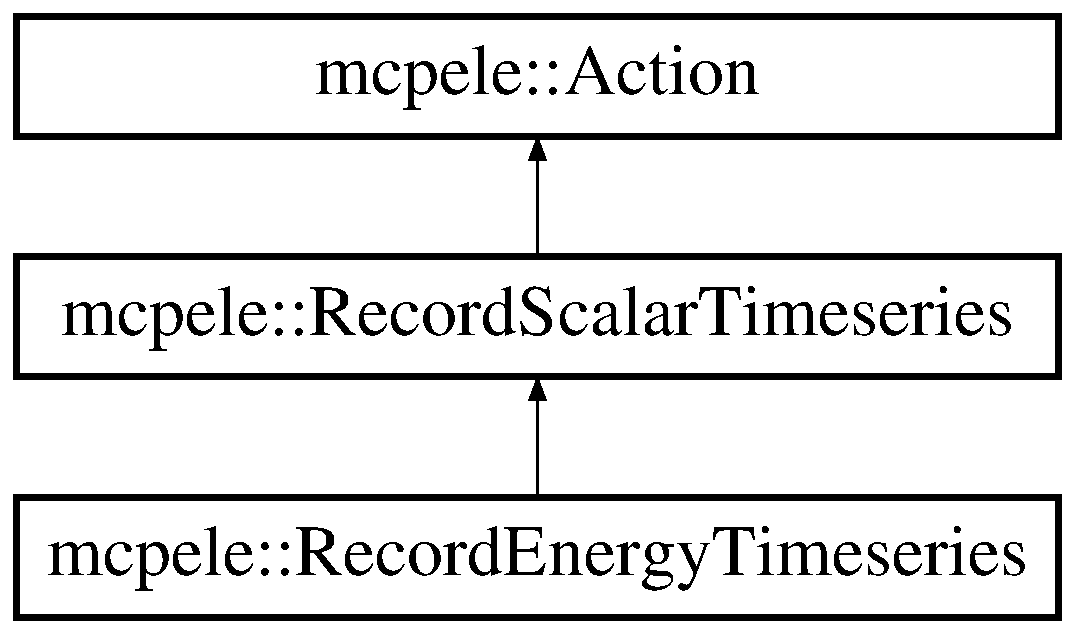
\includegraphics[height=3.000000cm]{classmcpele_1_1RecordEnergyTimeseries}
\end{center}
\end{figure}
\subsection*{\-Public \-Member \-Functions}
\begin{DoxyCompactItemize}
\item 
\hyperlink{classmcpele_1_1RecordEnergyTimeseries_a5e27f7e13a2c2357016f165c75f7e5ef}{\-Record\-Energy\-Timeseries} (const size\-\_\-t niter, const size\-\_\-t record\-\_\-every)
\item 
virtual \hyperlink{classmcpele_1_1RecordEnergyTimeseries_a19a365154f144b892095ef75034e6c88}{$\sim$\-Record\-Energy\-Timeseries} ()
\item 
virtual double \hyperlink{classmcpele_1_1RecordEnergyTimeseries_a6cab4a7ab5462ee3ddf0c6eacb88b757}{get\-\_\-recorded\-\_\-scalar} (pele\-::\-Array$<$ double $>$ \&coords, const double energy, const bool accepted, \hyperlink{classmcpele_1_1MC}{\-M\-C} $\ast$mc)
\end{DoxyCompactItemize}


\subsection{\-Detailed \-Description}


\-Definition at line 8 of file record\-\_\-energy\-\_\-timeseries.\-h.



\subsection{\-Constructor \& \-Destructor \-Documentation}
\hypertarget{classmcpele_1_1RecordEnergyTimeseries_a5e27f7e13a2c2357016f165c75f7e5ef}{\index{mcpele\-::\-Record\-Energy\-Timeseries@{mcpele\-::\-Record\-Energy\-Timeseries}!\-Record\-Energy\-Timeseries@{\-Record\-Energy\-Timeseries}}
\index{\-Record\-Energy\-Timeseries@{\-Record\-Energy\-Timeseries}!mcpele::RecordEnergyTimeseries@{mcpele\-::\-Record\-Energy\-Timeseries}}
\subsubsection[{\-Record\-Energy\-Timeseries}]{\setlength{\rightskip}{0pt plus 5cm}{\bf mcpele\-::\-Record\-Energy\-Timeseries\-::\-Record\-Energy\-Timeseries} (
\begin{DoxyParamCaption}
\item[{const size\-\_\-t}]{niter, }
\item[{const size\-\_\-t}]{record\-\_\-every}
\end{DoxyParamCaption}
)\hspace{0.3cm}{\ttfamily  \mbox{[}inline\mbox{]}}}}\label{classmcpele_1_1RecordEnergyTimeseries_a5e27f7e13a2c2357016f165c75f7e5ef}


\-Definition at line 10 of file record\-\_\-energy\-\_\-timeseries.\-h.

\hypertarget{classmcpele_1_1RecordEnergyTimeseries_a19a365154f144b892095ef75034e6c88}{\index{mcpele\-::\-Record\-Energy\-Timeseries@{mcpele\-::\-Record\-Energy\-Timeseries}!$\sim$\-Record\-Energy\-Timeseries@{$\sim$\-Record\-Energy\-Timeseries}}
\index{$\sim$\-Record\-Energy\-Timeseries@{$\sim$\-Record\-Energy\-Timeseries}!mcpele::RecordEnergyTimeseries@{mcpele\-::\-Record\-Energy\-Timeseries}}
\subsubsection[{$\sim$\-Record\-Energy\-Timeseries}]{\setlength{\rightskip}{0pt plus 5cm}virtual {\bf mcpele\-::\-Record\-Energy\-Timeseries\-::$\sim$\-Record\-Energy\-Timeseries} (
\begin{DoxyParamCaption}
{}
\end{DoxyParamCaption}
)\hspace{0.3cm}{\ttfamily  \mbox{[}inline, virtual\mbox{]}}}}\label{classmcpele_1_1RecordEnergyTimeseries_a19a365154f144b892095ef75034e6c88}


\-Definition at line 13 of file record\-\_\-energy\-\_\-timeseries.\-h.



\subsection{\-Member \-Function \-Documentation}
\hypertarget{classmcpele_1_1RecordEnergyTimeseries_a6cab4a7ab5462ee3ddf0c6eacb88b757}{\index{mcpele\-::\-Record\-Energy\-Timeseries@{mcpele\-::\-Record\-Energy\-Timeseries}!get\-\_\-recorded\-\_\-scalar@{get\-\_\-recorded\-\_\-scalar}}
\index{get\-\_\-recorded\-\_\-scalar@{get\-\_\-recorded\-\_\-scalar}!mcpele::RecordEnergyTimeseries@{mcpele\-::\-Record\-Energy\-Timeseries}}
\subsubsection[{get\-\_\-recorded\-\_\-scalar}]{\setlength{\rightskip}{0pt plus 5cm}virtual double {\bf mcpele\-::\-Record\-Energy\-Timeseries\-::get\-\_\-recorded\-\_\-scalar} (
\begin{DoxyParamCaption}
\item[{pele\-::\-Array$<$ double $>$ \&}]{coords, }
\item[{const double}]{energy, }
\item[{const bool}]{accepted, }
\item[{{\bf \-M\-C} $\ast$}]{mc}
\end{DoxyParamCaption}
)\hspace{0.3cm}{\ttfamily  \mbox{[}inline, virtual\mbox{]}}}}\label{classmcpele_1_1RecordEnergyTimeseries_a6cab4a7ab5462ee3ddf0c6eacb88b757}


\-Implements \hyperlink{classmcpele_1_1RecordScalarTimeseries_a8151f9f679c926d481e7354ac170663a}{mcpele\-::\-Record\-Scalar\-Timeseries}.



\-Definition at line 14 of file record\-\_\-energy\-\_\-timeseries.\-h.



\-The documentation for this class was generated from the following file\-:\begin{DoxyCompactItemize}
\item 
mcpele/\hyperlink{record__energy__timeseries_8h}{record\-\_\-energy\-\_\-timeseries.\-h}\end{DoxyCompactItemize}

\hypertarget{classmcpele_1_1RecordLowestEValueTimeseries}{\section{mcpele\-:\-:\-Record\-Lowest\-E\-Value\-Timeseries \-Class \-Reference}
\label{classmcpele_1_1RecordLowestEValueTimeseries}\index{mcpele\-::\-Record\-Lowest\-E\-Value\-Timeseries@{mcpele\-::\-Record\-Lowest\-E\-Value\-Timeseries}}
}


{\ttfamily \#include $<$record\-\_\-lowest\-\_\-evalue\-\_\-timeseries.\-h$>$}

\-Inheritance diagram for mcpele\-:\-:\-Record\-Lowest\-E\-Value\-Timeseries\-:\begin{figure}[H]
\begin{center}
\leavevmode
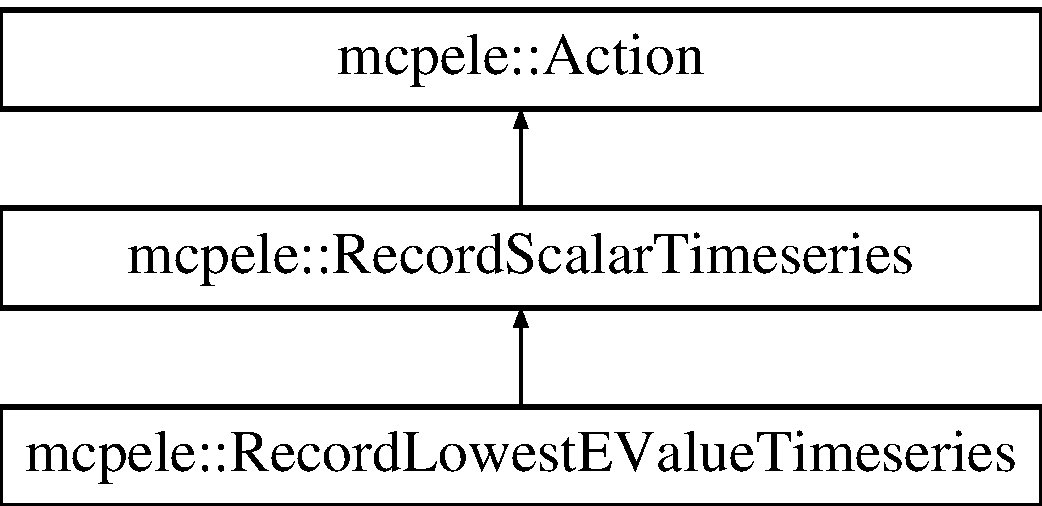
\includegraphics[height=3.000000cm]{classmcpele_1_1RecordLowestEValueTimeseries}
\end{center}
\end{figure}
\subsection*{\-Public \-Member \-Functions}
\begin{DoxyCompactItemize}
\item 
\hyperlink{classmcpele_1_1RecordLowestEValueTimeseries_a9ab99a86595a3620babe35e5e1e26083}{\-Record\-Lowest\-E\-Value\-Timeseries} (const size\-\_\-t niter, const size\-\_\-t record\-\_\-every, std\-::shared\-\_\-ptr$<$ pele\-::\-Base\-Potential $>$ landscape\-\_\-potential, const size\-\_\-t boxdimension, pele\-::\-Array$<$ double $>$ ranvec, const size\-\_\-t lbfgsniter=30)
\item 
virtual \hyperlink{classmcpele_1_1RecordLowestEValueTimeseries_a90ba22381fd38a8fff5adced32a2a64f}{$\sim$\-Record\-Lowest\-E\-Value\-Timeseries} ()
\item 
virtual double \hyperlink{classmcpele_1_1RecordLowestEValueTimeseries_affb535be88d9352a5b323e26a7c17bd2}{get\-\_\-recorded\-\_\-scalar} (pele\-::\-Array$<$ double $>$ \&coords, const double energy, const bool accepted, \hyperlink{classmcpele_1_1MC}{\-M\-C} $\ast$mc)
\end{DoxyCompactItemize}


\subsection{\-Detailed \-Description}
\-Record time series of lowest eigenvalue 

\-Definition at line 13 of file record\-\_\-lowest\-\_\-evalue\-\_\-timeseries.\-h.



\subsection{\-Constructor \& \-Destructor \-Documentation}
\hypertarget{classmcpele_1_1RecordLowestEValueTimeseries_a9ab99a86595a3620babe35e5e1e26083}{\index{mcpele\-::\-Record\-Lowest\-E\-Value\-Timeseries@{mcpele\-::\-Record\-Lowest\-E\-Value\-Timeseries}!\-Record\-Lowest\-E\-Value\-Timeseries@{\-Record\-Lowest\-E\-Value\-Timeseries}}
\index{\-Record\-Lowest\-E\-Value\-Timeseries@{\-Record\-Lowest\-E\-Value\-Timeseries}!mcpele::RecordLowestEValueTimeseries@{mcpele\-::\-Record\-Lowest\-E\-Value\-Timeseries}}
\subsubsection[{\-Record\-Lowest\-E\-Value\-Timeseries}]{\setlength{\rightskip}{0pt plus 5cm}{\bf mcpele\-::\-Record\-Lowest\-E\-Value\-Timeseries\-::\-Record\-Lowest\-E\-Value\-Timeseries} (
\begin{DoxyParamCaption}
\item[{const size\-\_\-t}]{niter, }
\item[{const size\-\_\-t}]{record\-\_\-every, }
\item[{std\-::shared\-\_\-ptr$<$ pele\-::\-Base\-Potential $>$}]{landscape\-\_\-potential, }
\item[{const size\-\_\-t}]{boxdimension, }
\item[{pele\-::\-Array$<$ double $>$}]{ranvec, }
\item[{const size\-\_\-t}]{lbfgsniter = {\ttfamily 30}}
\end{DoxyParamCaption}
)\hspace{0.3cm}{\ttfamily  \mbox{[}inline\mbox{]}}}}\label{classmcpele_1_1RecordLowestEValueTimeseries_a9ab99a86595a3620babe35e5e1e26083}


\-Definition at line 17 of file record\-\_\-lowest\-\_\-evalue\-\_\-timeseries.\-h.

\hypertarget{classmcpele_1_1RecordLowestEValueTimeseries_a90ba22381fd38a8fff5adced32a2a64f}{\index{mcpele\-::\-Record\-Lowest\-E\-Value\-Timeseries@{mcpele\-::\-Record\-Lowest\-E\-Value\-Timeseries}!$\sim$\-Record\-Lowest\-E\-Value\-Timeseries@{$\sim$\-Record\-Lowest\-E\-Value\-Timeseries}}
\index{$\sim$\-Record\-Lowest\-E\-Value\-Timeseries@{$\sim$\-Record\-Lowest\-E\-Value\-Timeseries}!mcpele::RecordLowestEValueTimeseries@{mcpele\-::\-Record\-Lowest\-E\-Value\-Timeseries}}
\subsubsection[{$\sim$\-Record\-Lowest\-E\-Value\-Timeseries}]{\setlength{\rightskip}{0pt plus 5cm}virtual {\bf mcpele\-::\-Record\-Lowest\-E\-Value\-Timeseries\-::$\sim$\-Record\-Lowest\-E\-Value\-Timeseries} (
\begin{DoxyParamCaption}
{}
\end{DoxyParamCaption}
)\hspace{0.3cm}{\ttfamily  \mbox{[}inline, virtual\mbox{]}}}}\label{classmcpele_1_1RecordLowestEValueTimeseries_a90ba22381fd38a8fff5adced32a2a64f}


\-Definition at line 25 of file record\-\_\-lowest\-\_\-evalue\-\_\-timeseries.\-h.



\subsection{\-Member \-Function \-Documentation}
\hypertarget{classmcpele_1_1RecordLowestEValueTimeseries_affb535be88d9352a5b323e26a7c17bd2}{\index{mcpele\-::\-Record\-Lowest\-E\-Value\-Timeseries@{mcpele\-::\-Record\-Lowest\-E\-Value\-Timeseries}!get\-\_\-recorded\-\_\-scalar@{get\-\_\-recorded\-\_\-scalar}}
\index{get\-\_\-recorded\-\_\-scalar@{get\-\_\-recorded\-\_\-scalar}!mcpele::RecordLowestEValueTimeseries@{mcpele\-::\-Record\-Lowest\-E\-Value\-Timeseries}}
\subsubsection[{get\-\_\-recorded\-\_\-scalar}]{\setlength{\rightskip}{0pt plus 5cm}virtual double {\bf mcpele\-::\-Record\-Lowest\-E\-Value\-Timeseries\-::get\-\_\-recorded\-\_\-scalar} (
\begin{DoxyParamCaption}
\item[{pele\-::\-Array$<$ double $>$ \&}]{coords, }
\item[{const double}]{energy, }
\item[{const bool}]{accepted, }
\item[{{\bf \-M\-C} $\ast$}]{mc}
\end{DoxyParamCaption}
)\hspace{0.3cm}{\ttfamily  \mbox{[}inline, virtual\mbox{]}}}}\label{classmcpele_1_1RecordLowestEValueTimeseries_affb535be88d9352a5b323e26a7c17bd2}


\-Implements \hyperlink{classmcpele_1_1RecordScalarTimeseries_a8151f9f679c926d481e7354ac170663a}{mcpele\-::\-Record\-Scalar\-Timeseries}.



\-Definition at line 26 of file record\-\_\-lowest\-\_\-evalue\-\_\-timeseries.\-h.



\-The documentation for this class was generated from the following file\-:\begin{DoxyCompactItemize}
\item 
mcpele/\hyperlink{record__lowest__evalue__timeseries_8h}{record\-\_\-lowest\-\_\-evalue\-\_\-timeseries.\-h}\end{DoxyCompactItemize}

\hypertarget{classmcpele_1_1RecordPairDistHistogram}{\section{mcpele\-:\-:\-Record\-Pair\-Dist\-Histogram$<$ \-B\-O\-X\-D\-I\-M $>$ \-Class \-Template \-Reference}
\label{classmcpele_1_1RecordPairDistHistogram}\index{mcpele\-::\-Record\-Pair\-Dist\-Histogram$<$ B\-O\-X\-D\-I\-M $>$@{mcpele\-::\-Record\-Pair\-Dist\-Histogram$<$ B\-O\-X\-D\-I\-M $>$}}
}


{\ttfamily \#include $<$record\-\_\-pair\-\_\-dist\-\_\-histogram.\-h$>$}

\-Inheritance diagram for mcpele\-:\-:\-Record\-Pair\-Dist\-Histogram$<$ \-B\-O\-X\-D\-I\-M $>$\-:\begin{figure}[H]
\begin{center}
\leavevmode
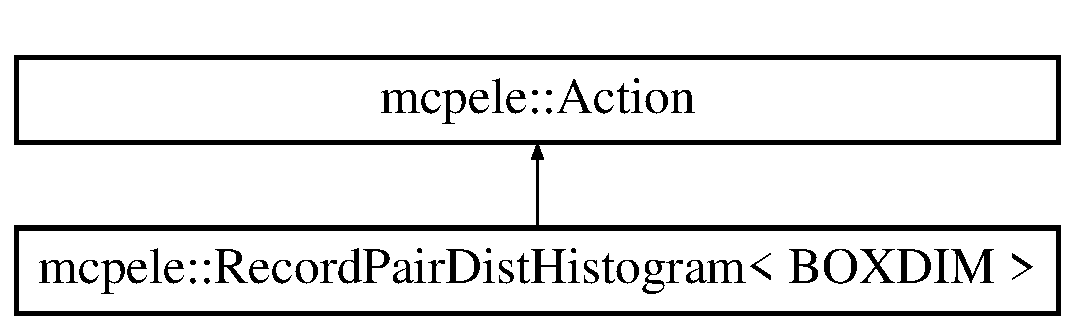
\includegraphics[height=2.000000cm]{classmcpele_1_1RecordPairDistHistogram}
\end{center}
\end{figure}
\subsection*{\-Public \-Member \-Functions}
\begin{DoxyCompactItemize}
\item 
\hyperlink{classmcpele_1_1RecordPairDistHistogram_a8c9dd2de7672d3858e7adf298fbf9c1b}{\-Record\-Pair\-Dist\-Histogram} (pele\-::\-Array$<$ double $>$ boxvector, const size\-\_\-t nr\-\_\-bins, const size\-\_\-t eqsteps, const size\-\_\-t record\-\_\-every)
\item 
virtual \hyperlink{classmcpele_1_1RecordPairDistHistogram_a5c084f8196fff90ea8dcfa9d61fa6d34}{$\sim$\-Record\-Pair\-Dist\-Histogram} ()
\item 
virtual void \hyperlink{classmcpele_1_1RecordPairDistHistogram_a2b0d3af344db398ce16e0a473f7f55c4}{action} (pele\-::\-Array$<$ double $>$ \&coords, double energy, bool accepted, \hyperlink{classmcpele_1_1MC}{\-M\-C} $\ast$mc)
\item 
size\-\_\-t \hyperlink{classmcpele_1_1RecordPairDistHistogram_a58689e61e83ea1223f322bbc20795d0e}{get\-\_\-eqsteps} () const 
\item 
pele\-::\-Array$<$ double $>$ \hyperlink{classmcpele_1_1RecordPairDistHistogram_a33de592d9288de540fc56edfecfbc8f1}{get\-\_\-hist\-\_\-r} () const 
\item 
pele\-::\-Array$<$ double $>$ \hyperlink{classmcpele_1_1RecordPairDistHistogram_ae8e88de17c1654b06412b73b1f9ad9e0}{get\-\_\-hist\-\_\-gr} (const double number\-\_\-density, const size\-\_\-t nr\-\_\-particles) const 
\end{DoxyCompactItemize}


\subsection{\-Detailed \-Description}
\subsubsection*{template$<$size\-\_\-t \-B\-O\-X\-D\-I\-M$>$class mcpele\-::\-Record\-Pair\-Dist\-Histogram$<$ B\-O\-X\-D\-I\-M $>$}

\-Record pair-\/distance distribution (radial distribution function) \-Templated on boxdimension, should work fine with pele\-::periodic\-\_\-distance \-Input parameters\-: -\/-\/-\/ boxvector\-: defines the (periodic) simlation box -\/-\/-\/ nr\-\_\-bins\-: number of bins for g(r) histogram -\/-\/-\/ eqsteps\-: number of equilibration steps to be excluded from g(r) computation -\/-\/-\/ record\-\_\-every\-: after more than eqsteps steps have been done, record every record\-\_\-everyth step \-Everytime the action is called, it accumulates the present configuration into the same g(r) histogram. \-The action function calls add\-\_\-configuration which accumulates the current configuration into the g(r) histogram. \-The g(r) histogram can be read out at any point after that. \-To read out the data, two functions are used\-: -\/-\/-\/ \hyperlink{classmcpele_1_1RecordPairDistHistogram_a33de592d9288de540fc56edfecfbc8f1}{get\-\_\-hist\-\_\-r()} gives the r value array for the g(r) histogram -\/-\/-\/ \hyperlink{classmcpele_1_1RecordPairDistHistogram_ae8e88de17c1654b06412b73b1f9ad9e0}{get\-\_\-hist\-\_\-gr()} gives the corresponding g(r) value array, normalized using the input number of particles and number density (\-Admittedly number density could have been reconstructed independently of that input.) 

\-Definition at line 27 of file record\-\_\-pair\-\_\-dist\-\_\-histogram.\-h.



\subsection{\-Constructor \& \-Destructor \-Documentation}
\hypertarget{classmcpele_1_1RecordPairDistHistogram_a8c9dd2de7672d3858e7adf298fbf9c1b}{\index{mcpele\-::\-Record\-Pair\-Dist\-Histogram@{mcpele\-::\-Record\-Pair\-Dist\-Histogram}!\-Record\-Pair\-Dist\-Histogram@{\-Record\-Pair\-Dist\-Histogram}}
\index{\-Record\-Pair\-Dist\-Histogram@{\-Record\-Pair\-Dist\-Histogram}!mcpele::RecordPairDistHistogram@{mcpele\-::\-Record\-Pair\-Dist\-Histogram}}
\subsubsection[{\-Record\-Pair\-Dist\-Histogram}]{\setlength{\rightskip}{0pt plus 5cm}template$<$size\-\_\-t \-B\-O\-X\-D\-I\-M$>$ {\bf mcpele\-::\-Record\-Pair\-Dist\-Histogram}$<$ \-B\-O\-X\-D\-I\-M $>$\-::{\bf \-Record\-Pair\-Dist\-Histogram} (
\begin{DoxyParamCaption}
\item[{pele\-::\-Array$<$ double $>$}]{boxvector, }
\item[{const size\-\_\-t}]{nr\-\_\-bins, }
\item[{const size\-\_\-t}]{eqsteps, }
\item[{const size\-\_\-t}]{record\-\_\-every}
\end{DoxyParamCaption}
)\hspace{0.3cm}{\ttfamily  \mbox{[}inline\mbox{]}}}}\label{classmcpele_1_1RecordPairDistHistogram_a8c9dd2de7672d3858e7adf298fbf9c1b}


\-Definition at line 33 of file record\-\_\-pair\-\_\-dist\-\_\-histogram.\-h.

\hypertarget{classmcpele_1_1RecordPairDistHistogram_a5c084f8196fff90ea8dcfa9d61fa6d34}{\index{mcpele\-::\-Record\-Pair\-Dist\-Histogram@{mcpele\-::\-Record\-Pair\-Dist\-Histogram}!$\sim$\-Record\-Pair\-Dist\-Histogram@{$\sim$\-Record\-Pair\-Dist\-Histogram}}
\index{$\sim$\-Record\-Pair\-Dist\-Histogram@{$\sim$\-Record\-Pair\-Dist\-Histogram}!mcpele::RecordPairDistHistogram@{mcpele\-::\-Record\-Pair\-Dist\-Histogram}}
\subsubsection[{$\sim$\-Record\-Pair\-Dist\-Histogram}]{\setlength{\rightskip}{0pt plus 5cm}template$<$size\-\_\-t \-B\-O\-X\-D\-I\-M$>$ virtual {\bf mcpele\-::\-Record\-Pair\-Dist\-Histogram}$<$ \-B\-O\-X\-D\-I\-M $>$\-::$\sim${\bf \-Record\-Pair\-Dist\-Histogram} (
\begin{DoxyParamCaption}
{}
\end{DoxyParamCaption}
)\hspace{0.3cm}{\ttfamily  \mbox{[}inline, virtual\mbox{]}}}}\label{classmcpele_1_1RecordPairDistHistogram_a5c084f8196fff90ea8dcfa9d61fa6d34}


\-Definition at line 38 of file record\-\_\-pair\-\_\-dist\-\_\-histogram.\-h.



\subsection{\-Member \-Function \-Documentation}
\hypertarget{classmcpele_1_1RecordPairDistHistogram_a2b0d3af344db398ce16e0a473f7f55c4}{\index{mcpele\-::\-Record\-Pair\-Dist\-Histogram@{mcpele\-::\-Record\-Pair\-Dist\-Histogram}!action@{action}}
\index{action@{action}!mcpele::RecordPairDistHistogram@{mcpele\-::\-Record\-Pair\-Dist\-Histogram}}
\subsubsection[{action}]{\setlength{\rightskip}{0pt plus 5cm}template$<$size\-\_\-t \-B\-O\-X\-D\-I\-M$>$ virtual void {\bf mcpele\-::\-Record\-Pair\-Dist\-Histogram}$<$ \-B\-O\-X\-D\-I\-M $>$\-::{\bf action} (
\begin{DoxyParamCaption}
\item[{pele\-::\-Array$<$ double $>$ \&}]{coords, }
\item[{double}]{energy, }
\item[{bool}]{accepted, }
\item[{{\bf \-M\-C} $\ast$}]{mc}
\end{DoxyParamCaption}
)\hspace{0.3cm}{\ttfamily  \mbox{[}inline, virtual\mbox{]}}}}\label{classmcpele_1_1RecordPairDistHistogram_a2b0d3af344db398ce16e0a473f7f55c4}


\-Implements \hyperlink{classmcpele_1_1Action_a9500d60c55f0d36ffb6ed0464ea3c68e}{mcpele\-::\-Action}.



\-Definition at line 39 of file record\-\_\-pair\-\_\-dist\-\_\-histogram.\-h.

\hypertarget{classmcpele_1_1RecordPairDistHistogram_a58689e61e83ea1223f322bbc20795d0e}{\index{mcpele\-::\-Record\-Pair\-Dist\-Histogram@{mcpele\-::\-Record\-Pair\-Dist\-Histogram}!get\-\_\-eqsteps@{get\-\_\-eqsteps}}
\index{get\-\_\-eqsteps@{get\-\_\-eqsteps}!mcpele::RecordPairDistHistogram@{mcpele\-::\-Record\-Pair\-Dist\-Histogram}}
\subsubsection[{get\-\_\-eqsteps}]{\setlength{\rightskip}{0pt plus 5cm}template$<$size\-\_\-t \-B\-O\-X\-D\-I\-M$>$ size\-\_\-t {\bf mcpele\-::\-Record\-Pair\-Dist\-Histogram}$<$ \-B\-O\-X\-D\-I\-M $>$\-::{\bf get\-\_\-eqsteps} (
\begin{DoxyParamCaption}
{}
\end{DoxyParamCaption}
) const\hspace{0.3cm}{\ttfamily  \mbox{[}inline\mbox{]}}}}\label{classmcpele_1_1RecordPairDistHistogram_a58689e61e83ea1223f322bbc20795d0e}


\-Definition at line 48 of file record\-\_\-pair\-\_\-dist\-\_\-histogram.\-h.

\hypertarget{classmcpele_1_1RecordPairDistHistogram_ae8e88de17c1654b06412b73b1f9ad9e0}{\index{mcpele\-::\-Record\-Pair\-Dist\-Histogram@{mcpele\-::\-Record\-Pair\-Dist\-Histogram}!get\-\_\-hist\-\_\-gr@{get\-\_\-hist\-\_\-gr}}
\index{get\-\_\-hist\-\_\-gr@{get\-\_\-hist\-\_\-gr}!mcpele::RecordPairDistHistogram@{mcpele\-::\-Record\-Pair\-Dist\-Histogram}}
\subsubsection[{get\-\_\-hist\-\_\-gr}]{\setlength{\rightskip}{0pt plus 5cm}template$<$size\-\_\-t \-B\-O\-X\-D\-I\-M$>$ pele\-::\-Array$<$double$>$ {\bf mcpele\-::\-Record\-Pair\-Dist\-Histogram}$<$ \-B\-O\-X\-D\-I\-M $>$\-::{\bf get\-\_\-hist\-\_\-gr} (
\begin{DoxyParamCaption}
\item[{const double}]{number\-\_\-density, }
\item[{const size\-\_\-t}]{nr\-\_\-particles}
\end{DoxyParamCaption}
) const\hspace{0.3cm}{\ttfamily  \mbox{[}inline\mbox{]}}}}\label{classmcpele_1_1RecordPairDistHistogram_ae8e88de17c1654b06412b73b1f9ad9e0}


\-Definition at line 57 of file record\-\_\-pair\-\_\-dist\-\_\-histogram.\-h.

\hypertarget{classmcpele_1_1RecordPairDistHistogram_a33de592d9288de540fc56edfecfbc8f1}{\index{mcpele\-::\-Record\-Pair\-Dist\-Histogram@{mcpele\-::\-Record\-Pair\-Dist\-Histogram}!get\-\_\-hist\-\_\-r@{get\-\_\-hist\-\_\-r}}
\index{get\-\_\-hist\-\_\-r@{get\-\_\-hist\-\_\-r}!mcpele::RecordPairDistHistogram@{mcpele\-::\-Record\-Pair\-Dist\-Histogram}}
\subsubsection[{get\-\_\-hist\-\_\-r}]{\setlength{\rightskip}{0pt plus 5cm}template$<$size\-\_\-t \-B\-O\-X\-D\-I\-M$>$ pele\-::\-Array$<$double$>$ {\bf mcpele\-::\-Record\-Pair\-Dist\-Histogram}$<$ \-B\-O\-X\-D\-I\-M $>$\-::{\bf get\-\_\-hist\-\_\-r} (
\begin{DoxyParamCaption}
{}
\end{DoxyParamCaption}
) const\hspace{0.3cm}{\ttfamily  \mbox{[}inline\mbox{]}}}}\label{classmcpele_1_1RecordPairDistHistogram_a33de592d9288de540fc56edfecfbc8f1}


\-Definition at line 52 of file record\-\_\-pair\-\_\-dist\-\_\-histogram.\-h.



\-The documentation for this class was generated from the following file\-:\begin{DoxyCompactItemize}
\item 
mcpele/\hyperlink{record__pair__dist__histogram_8h}{record\-\_\-pair\-\_\-dist\-\_\-histogram.\-h}\end{DoxyCompactItemize}

\hypertarget{classmcpele_1_1RecordScalarTimeseries}{\section{mcpele\-:\-:\-Record\-Scalar\-Timeseries \-Class \-Reference}
\label{classmcpele_1_1RecordScalarTimeseries}\index{mcpele\-::\-Record\-Scalar\-Timeseries@{mcpele\-::\-Record\-Scalar\-Timeseries}}
}


{\ttfamily \#include $<$record\-\_\-scalar\-\_\-timeseries.\-h$>$}

\-Inheritance diagram for mcpele\-:\-:\-Record\-Scalar\-Timeseries\-:\begin{figure}[H]
\begin{center}
\leavevmode
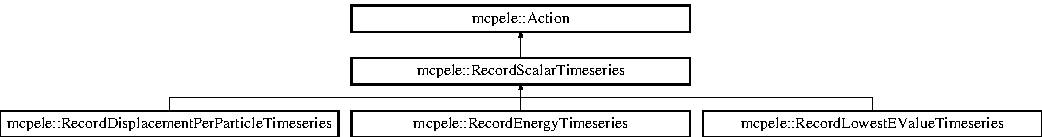
\includegraphics[height=1.836066cm]{classmcpele_1_1RecordScalarTimeseries}
\end{center}
\end{figure}
\subsection*{\-Public \-Member \-Functions}
\begin{DoxyCompactItemize}
\item 
\hyperlink{classmcpele_1_1RecordScalarTimeseries_af446b764d9a8f16f67c751bfb94a47d1}{\-Record\-Scalar\-Timeseries} (const size\-\_\-t, const size\-\_\-t)
\item 
virtual \hyperlink{classmcpele_1_1RecordScalarTimeseries_aba51863fc7829b1fa7a2908ea3b8dd3c}{$\sim$\-Record\-Scalar\-Timeseries} ()
\item 
virtual void \hyperlink{classmcpele_1_1RecordScalarTimeseries_a7cc733d8f0b8daebf4da92423793b9c7}{action} (pele\-::\-Array$<$ double $>$ \&coords, double energy, bool accepted, \hyperlink{classmcpele_1_1MC}{\-M\-C} $\ast$mc)
\item 
virtual double \hyperlink{classmcpele_1_1RecordScalarTimeseries_a8151f9f679c926d481e7354ac170663a}{get\-\_\-recorded\-\_\-scalar} (pele\-::\-Array$<$ double $>$ \&coords, const double energy, const bool accepted, \hyperlink{classmcpele_1_1MC}{\-M\-C} $\ast$mc)=0
\item 
bool \hyperlink{classmcpele_1_1RecordScalarTimeseries_a98fce48e1cc8cd2e73fb0705a4d05cde}{moving\-\_\-average\-\_\-is\-\_\-stable} (const size\-\_\-t nr\-\_\-steps\-\_\-to\-\_\-check=1000, const double rel\-\_\-std\-\_\-threshold=0.\-1)
\item 
std\-::pair$<$ double, double $>$ \hyperlink{classmcpele_1_1RecordScalarTimeseries_aa5cce7dde2ec7f096baeefad210ff063}{get\-\_\-moving\-\_\-average\-\_\-mean} (const size\-\_\-t nr\-\_\-steps\-\_\-to\-\_\-check)
\item 
std\-::pair$<$ double, double $>$ \hyperlink{classmcpele_1_1RecordScalarTimeseries_a0df1f17ac9304e831f37e7e97bf45b83}{get\-\_\-moving\-\_\-average\-\_\-variance} (const size\-\_\-t nr\-\_\-steps\-\_\-to\-\_\-check)
\item 
pele\-::\-Array$<$ double $>$ \hyperlink{classmcpele_1_1RecordScalarTimeseries_ad3c2dbc09a421030dcddff87d96299e5}{get\-\_\-time\-\_\-series} ()
\item 
void \hyperlink{classmcpele_1_1RecordScalarTimeseries_a0f616cd3a4e0dea710c0919f22b8f5ce}{clear} ()
\end{DoxyCompactItemize}


\subsection{\-Detailed \-Description}
\-Record scalar time series, every record\-\_\-every-\/th step. 

\-Definition at line 11 of file record\-\_\-scalar\-\_\-timeseries.\-h.



\subsection{\-Constructor \& \-Destructor \-Documentation}
\hypertarget{classmcpele_1_1RecordScalarTimeseries_af446b764d9a8f16f67c751bfb94a47d1}{\index{mcpele\-::\-Record\-Scalar\-Timeseries@{mcpele\-::\-Record\-Scalar\-Timeseries}!\-Record\-Scalar\-Timeseries@{\-Record\-Scalar\-Timeseries}}
\index{\-Record\-Scalar\-Timeseries@{\-Record\-Scalar\-Timeseries}!mcpele::RecordScalarTimeseries@{mcpele\-::\-Record\-Scalar\-Timeseries}}
\subsubsection[{\-Record\-Scalar\-Timeseries}]{\setlength{\rightskip}{0pt plus 5cm}{\bf mcpele\-::\-Record\-Scalar\-Timeseries\-::\-Record\-Scalar\-Timeseries} (
\begin{DoxyParamCaption}
\item[{const size\-\_\-t}]{niter, }
\item[{const size\-\_\-t}]{record\-\_\-every}
\end{DoxyParamCaption}
)}}\label{classmcpele_1_1RecordScalarTimeseries_af446b764d9a8f16f67c751bfb94a47d1}


\-Definition at line 8 of file record\-\_\-scalar\-\_\-timeseries.\-cpp.

\hypertarget{classmcpele_1_1RecordScalarTimeseries_aba51863fc7829b1fa7a2908ea3b8dd3c}{\index{mcpele\-::\-Record\-Scalar\-Timeseries@{mcpele\-::\-Record\-Scalar\-Timeseries}!$\sim$\-Record\-Scalar\-Timeseries@{$\sim$\-Record\-Scalar\-Timeseries}}
\index{$\sim$\-Record\-Scalar\-Timeseries@{$\sim$\-Record\-Scalar\-Timeseries}!mcpele::RecordScalarTimeseries@{mcpele\-::\-Record\-Scalar\-Timeseries}}
\subsubsection[{$\sim$\-Record\-Scalar\-Timeseries}]{\setlength{\rightskip}{0pt plus 5cm}virtual {\bf mcpele\-::\-Record\-Scalar\-Timeseries\-::$\sim$\-Record\-Scalar\-Timeseries} (
\begin{DoxyParamCaption}
{}
\end{DoxyParamCaption}
)\hspace{0.3cm}{\ttfamily  \mbox{[}inline, virtual\mbox{]}}}}\label{classmcpele_1_1RecordScalarTimeseries_aba51863fc7829b1fa7a2908ea3b8dd3c}


\-Definition at line 21 of file record\-\_\-scalar\-\_\-timeseries.\-h.



\subsection{\-Member \-Function \-Documentation}
\hypertarget{classmcpele_1_1RecordScalarTimeseries_a7cc733d8f0b8daebf4da92423793b9c7}{\index{mcpele\-::\-Record\-Scalar\-Timeseries@{mcpele\-::\-Record\-Scalar\-Timeseries}!action@{action}}
\index{action@{action}!mcpele::RecordScalarTimeseries@{mcpele\-::\-Record\-Scalar\-Timeseries}}
\subsubsection[{action}]{\setlength{\rightskip}{0pt plus 5cm}void {\bf mcpele\-::\-Record\-Scalar\-Timeseries\-::action} (
\begin{DoxyParamCaption}
\item[{pele\-::\-Array$<$ double $>$ \&}]{coords, }
\item[{double}]{energy, }
\item[{bool}]{accepted, }
\item[{{\bf \-M\-C} $\ast$}]{mc}
\end{DoxyParamCaption}
)\hspace{0.3cm}{\ttfamily  \mbox{[}virtual\mbox{]}}}}\label{classmcpele_1_1RecordScalarTimeseries_a7cc733d8f0b8daebf4da92423793b9c7}


\-Implements \hyperlink{classmcpele_1_1Action_a9500d60c55f0d36ffb6ed0464ea3c68e}{mcpele\-::\-Action}.



\-Definition at line 17 of file record\-\_\-scalar\-\_\-timeseries.\-cpp.

\hypertarget{classmcpele_1_1RecordScalarTimeseries_a0f616cd3a4e0dea710c0919f22b8f5ce}{\index{mcpele\-::\-Record\-Scalar\-Timeseries@{mcpele\-::\-Record\-Scalar\-Timeseries}!clear@{clear}}
\index{clear@{clear}!mcpele::RecordScalarTimeseries@{mcpele\-::\-Record\-Scalar\-Timeseries}}
\subsubsection[{clear}]{\setlength{\rightskip}{0pt plus 5cm}void {\bf mcpele\-::\-Record\-Scalar\-Timeseries\-::clear} (
\begin{DoxyParamCaption}
{}
\end{DoxyParamCaption}
)\hspace{0.3cm}{\ttfamily  \mbox{[}inline\mbox{]}}}}\label{classmcpele_1_1RecordScalarTimeseries_a0f616cd3a4e0dea710c0919f22b8f5ce}


\-Definition at line 32 of file record\-\_\-scalar\-\_\-timeseries.\-h.

\hypertarget{classmcpele_1_1RecordScalarTimeseries_aa5cce7dde2ec7f096baeefad210ff063}{\index{mcpele\-::\-Record\-Scalar\-Timeseries@{mcpele\-::\-Record\-Scalar\-Timeseries}!get\-\_\-moving\-\_\-average\-\_\-mean@{get\-\_\-moving\-\_\-average\-\_\-mean}}
\index{get\-\_\-moving\-\_\-average\-\_\-mean@{get\-\_\-moving\-\_\-average\-\_\-mean}!mcpele::RecordScalarTimeseries@{mcpele\-::\-Record\-Scalar\-Timeseries}}
\subsubsection[{get\-\_\-moving\-\_\-average\-\_\-mean}]{\setlength{\rightskip}{0pt plus 5cm}std\-::pair$<$ double, double $>$ {\bf mcpele\-::\-Record\-Scalar\-Timeseries\-::get\-\_\-moving\-\_\-average\-\_\-mean} (
\begin{DoxyParamCaption}
\item[{const size\-\_\-t}]{nr\-\_\-steps\-\_\-to\-\_\-check}
\end{DoxyParamCaption}
)}}\label{classmcpele_1_1RecordScalarTimeseries_aa5cce7dde2ec7f096baeefad210ff063}


\-Definition at line 55 of file record\-\_\-scalar\-\_\-timeseries.\-cpp.

\hypertarget{classmcpele_1_1RecordScalarTimeseries_a0df1f17ac9304e831f37e7e97bf45b83}{\index{mcpele\-::\-Record\-Scalar\-Timeseries@{mcpele\-::\-Record\-Scalar\-Timeseries}!get\-\_\-moving\-\_\-average\-\_\-variance@{get\-\_\-moving\-\_\-average\-\_\-variance}}
\index{get\-\_\-moving\-\_\-average\-\_\-variance@{get\-\_\-moving\-\_\-average\-\_\-variance}!mcpele::RecordScalarTimeseries@{mcpele\-::\-Record\-Scalar\-Timeseries}}
\subsubsection[{get\-\_\-moving\-\_\-average\-\_\-variance}]{\setlength{\rightskip}{0pt plus 5cm}std\-::pair$<$ double, double $>$ {\bf mcpele\-::\-Record\-Scalar\-Timeseries\-::get\-\_\-moving\-\_\-average\-\_\-variance} (
\begin{DoxyParamCaption}
\item[{const size\-\_\-t}]{nr\-\_\-steps\-\_\-to\-\_\-check}
\end{DoxyParamCaption}
)}}\label{classmcpele_1_1RecordScalarTimeseries_a0df1f17ac9304e831f37e7e97bf45b83}


\-Definition at line 69 of file record\-\_\-scalar\-\_\-timeseries.\-cpp.

\hypertarget{classmcpele_1_1RecordScalarTimeseries_a8151f9f679c926d481e7354ac170663a}{\index{mcpele\-::\-Record\-Scalar\-Timeseries@{mcpele\-::\-Record\-Scalar\-Timeseries}!get\-\_\-recorded\-\_\-scalar@{get\-\_\-recorded\-\_\-scalar}}
\index{get\-\_\-recorded\-\_\-scalar@{get\-\_\-recorded\-\_\-scalar}!mcpele::RecordScalarTimeseries@{mcpele\-::\-Record\-Scalar\-Timeseries}}
\subsubsection[{get\-\_\-recorded\-\_\-scalar}]{\setlength{\rightskip}{0pt plus 5cm}virtual double {\bf mcpele\-::\-Record\-Scalar\-Timeseries\-::get\-\_\-recorded\-\_\-scalar} (
\begin{DoxyParamCaption}
\item[{pele\-::\-Array$<$ double $>$ \&}]{coords, }
\item[{const double}]{energy, }
\item[{const bool}]{accepted, }
\item[{{\bf \-M\-C} $\ast$}]{mc}
\end{DoxyParamCaption}
)\hspace{0.3cm}{\ttfamily  \mbox{[}pure virtual\mbox{]}}}}\label{classmcpele_1_1RecordScalarTimeseries_a8151f9f679c926d481e7354ac170663a}


\-Implemented in \hyperlink{classmcpele_1_1RecordLowestEValueTimeseries_affb535be88d9352a5b323e26a7c17bd2}{mcpele\-::\-Record\-Lowest\-E\-Value\-Timeseries}, \hyperlink{classmcpele_1_1RecordDisplacementPerParticleTimeseries_ac049afa25de4847b76910680cb3f1a10}{mcpele\-::\-Record\-Displacement\-Per\-Particle\-Timeseries}, and \hyperlink{classmcpele_1_1RecordEnergyTimeseries_a6cab4a7ab5462ee3ddf0c6eacb88b757}{mcpele\-::\-Record\-Energy\-Timeseries}.

\hypertarget{classmcpele_1_1RecordScalarTimeseries_ad3c2dbc09a421030dcddff87d96299e5}{\index{mcpele\-::\-Record\-Scalar\-Timeseries@{mcpele\-::\-Record\-Scalar\-Timeseries}!get\-\_\-time\-\_\-series@{get\-\_\-time\-\_\-series}}
\index{get\-\_\-time\-\_\-series@{get\-\_\-time\-\_\-series}!mcpele::RecordScalarTimeseries@{mcpele\-::\-Record\-Scalar\-Timeseries}}
\subsubsection[{get\-\_\-time\-\_\-series}]{\setlength{\rightskip}{0pt plus 5cm}pele\-::\-Array$<$double$>$ {\bf mcpele\-::\-Record\-Scalar\-Timeseries\-::get\-\_\-time\-\_\-series} (
\begin{DoxyParamCaption}
{}
\end{DoxyParamCaption}
)\hspace{0.3cm}{\ttfamily  \mbox{[}inline\mbox{]}}}}\label{classmcpele_1_1RecordScalarTimeseries_ad3c2dbc09a421030dcddff87d96299e5}


\-Definition at line 27 of file record\-\_\-scalar\-\_\-timeseries.\-h.

\hypertarget{classmcpele_1_1RecordScalarTimeseries_a98fce48e1cc8cd2e73fb0705a4d05cde}{\index{mcpele\-::\-Record\-Scalar\-Timeseries@{mcpele\-::\-Record\-Scalar\-Timeseries}!moving\-\_\-average\-\_\-is\-\_\-stable@{moving\-\_\-average\-\_\-is\-\_\-stable}}
\index{moving\-\_\-average\-\_\-is\-\_\-stable@{moving\-\_\-average\-\_\-is\-\_\-stable}!mcpele::RecordScalarTimeseries@{mcpele\-::\-Record\-Scalar\-Timeseries}}
\subsubsection[{moving\-\_\-average\-\_\-is\-\_\-stable}]{\setlength{\rightskip}{0pt plus 5cm}bool {\bf mcpele\-::\-Record\-Scalar\-Timeseries\-::moving\-\_\-average\-\_\-is\-\_\-stable} (
\begin{DoxyParamCaption}
\item[{const size\-\_\-t}]{nr\-\_\-steps\-\_\-to\-\_\-check = {\ttfamily 1000}, }
\item[{const double}]{rel\-\_\-std\-\_\-threshold = {\ttfamily 0.1}}
\end{DoxyParamCaption}
)}}\label{classmcpele_1_1RecordScalarTimeseries_a98fce48e1cc8cd2e73fb0705a4d05cde}
\-Apply a basic check on the behaviour of the moving average of the recorded time series to decide if it is sufficiently stable. \-Parameters\-: nr\-\_\-steps\-\_\-to\-\_\-check is the number of steps, from the present into the past, that are considered for the moving average check. rel\-\_\-std\-\_\-threshold is the relative size of the fluctuations in the moving average that is considered stable. \-Decreasing that number should make the test more sensitive. \-N\-O\-T\-E\-: we do not test the variance because the variance has some functional dependence on the mean var = f(mu). \-In order to remove this one would require a \char`\"{}variance stabilising transformation\char`\"{} which would require the implementation of a different moments class where f(x) si stored giving an approximately constant variance as a function of the mean. \-See \-Ascombe transform for instance. 

\-Definition at line 40 of file record\-\_\-scalar\-\_\-timeseries.\-cpp.



\-The documentation for this class was generated from the following files\-:\begin{DoxyCompactItemize}
\item 
mcpele/\hyperlink{record__scalar__timeseries_8h}{record\-\_\-scalar\-\_\-timeseries.\-h}\item 
\hyperlink{record__scalar__timeseries_8cpp}{record\-\_\-scalar\-\_\-timeseries.\-cpp}\end{DoxyCompactItemize}

\hypertarget{classmcpele_1_1TakeStep}{\section{mcpele\-:\-:\-Take\-Step \-Class \-Reference}
\label{classmcpele_1_1TakeStep}\index{mcpele\-::\-Take\-Step@{mcpele\-::\-Take\-Step}}
}


{\ttfamily \#include $<$mc.\-h$>$}

\-Inheritance diagram for mcpele\-:\-:\-Take\-Step\-:\begin{figure}[H]
\begin{center}
\leavevmode
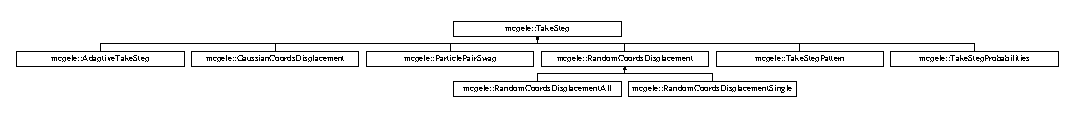
\includegraphics[height=1.068702cm]{classmcpele_1_1TakeStep}
\end{center}
\end{figure}
\subsection*{\-Public \-Member \-Functions}
\begin{DoxyCompactItemize}
\item 
virtual \hyperlink{classmcpele_1_1TakeStep_a82aab5c2527f8a7fd4c0f8a438dc3625}{$\sim$\-Take\-Step} ()
\item 
virtual void \hyperlink{classmcpele_1_1TakeStep_ac3032e0d99d4aa5f940ffea4a28442f5}{displace} (pele\-::\-Array$<$ double $>$ \&coords, \hyperlink{classmcpele_1_1MC}{\-M\-C} $\ast$mc)=0
\item 
virtual void \hyperlink{classmcpele_1_1TakeStep_aac4f30de62c4cbc4d9d31c7629742f64}{report} (pele\-::\-Array$<$ double $>$ \&, const double, pele\-::\-Array$<$ double $>$ \&, const double, const bool, \hyperlink{classmcpele_1_1MC}{\-M\-C} $\ast$)
\item 
virtual void \hyperlink{classmcpele_1_1TakeStep_afa92f5196e0304d6ad910304b188c705}{increase\-\_\-acceptance} (const double)
\item 
virtual void \hyperlink{classmcpele_1_1TakeStep_a492ccf2a2e3b3d8ef2224947d0385d77}{decrease\-\_\-acceptance} (const double)
\end{DoxyCompactItemize}


\subsection{\-Detailed \-Description}


\-Definition at line 59 of file mc.\-h.



\subsection{\-Constructor \& \-Destructor \-Documentation}
\hypertarget{classmcpele_1_1TakeStep_a82aab5c2527f8a7fd4c0f8a438dc3625}{\index{mcpele\-::\-Take\-Step@{mcpele\-::\-Take\-Step}!$\sim$\-Take\-Step@{$\sim$\-Take\-Step}}
\index{$\sim$\-Take\-Step@{$\sim$\-Take\-Step}!mcpele::TakeStep@{mcpele\-::\-Take\-Step}}
\subsubsection[{$\sim$\-Take\-Step}]{\setlength{\rightskip}{0pt plus 5cm}virtual {\bf mcpele\-::\-Take\-Step\-::$\sim$\-Take\-Step} (
\begin{DoxyParamCaption}
{}
\end{DoxyParamCaption}
)\hspace{0.3cm}{\ttfamily  \mbox{[}inline, virtual\mbox{]}}}}\label{classmcpele_1_1TakeStep_a82aab5c2527f8a7fd4c0f8a438dc3625}


\-Definition at line 61 of file mc.\-h.



\subsection{\-Member \-Function \-Documentation}
\hypertarget{classmcpele_1_1TakeStep_a492ccf2a2e3b3d8ef2224947d0385d77}{\index{mcpele\-::\-Take\-Step@{mcpele\-::\-Take\-Step}!decrease\-\_\-acceptance@{decrease\-\_\-acceptance}}
\index{decrease\-\_\-acceptance@{decrease\-\_\-acceptance}!mcpele::TakeStep@{mcpele\-::\-Take\-Step}}
\subsubsection[{decrease\-\_\-acceptance}]{\setlength{\rightskip}{0pt plus 5cm}virtual void {\bf mcpele\-::\-Take\-Step\-::decrease\-\_\-acceptance} (
\begin{DoxyParamCaption}
\item[{const double}]{}
\end{DoxyParamCaption}
)\hspace{0.3cm}{\ttfamily  \mbox{[}inline, virtual\mbox{]}}}}\label{classmcpele_1_1TakeStep_a492ccf2a2e3b3d8ef2224947d0385d77}


\-Reimplemented in \hyperlink{classmcpele_1_1RandomCoordsDisplacement_a75b39857737f466cee1ff4fe452d848e}{mcpele\-::\-Random\-Coords\-Displacement}.



\-Definition at line 66 of file mc.\-h.

\hypertarget{classmcpele_1_1TakeStep_ac3032e0d99d4aa5f940ffea4a28442f5}{\index{mcpele\-::\-Take\-Step@{mcpele\-::\-Take\-Step}!displace@{displace}}
\index{displace@{displace}!mcpele::TakeStep@{mcpele\-::\-Take\-Step}}
\subsubsection[{displace}]{\setlength{\rightskip}{0pt plus 5cm}virtual void {\bf mcpele\-::\-Take\-Step\-::displace} (
\begin{DoxyParamCaption}
\item[{pele\-::\-Array$<$ double $>$ \&}]{coords, }
\item[{{\bf \-M\-C} $\ast$}]{mc}
\end{DoxyParamCaption}
)\hspace{0.3cm}{\ttfamily  \mbox{[}pure virtual\mbox{]}}}}\label{classmcpele_1_1TakeStep_ac3032e0d99d4aa5f940ffea4a28442f5}


\-Implemented in \hyperlink{classmcpele_1_1RandomCoordsDisplacementSingle_a52c3271d105453d89024230f3f392dc7}{mcpele\-::\-Random\-Coords\-Displacement\-Single}, \hyperlink{classmcpele_1_1RandomCoordsDisplacementAll_ab40ce59b2d74ffe3d8042c3e90268eab}{mcpele\-::\-Random\-Coords\-Displacement\-All}, \hyperlink{classmcpele_1_1TakeStepPattern_a8c5ef12183c58b84b3ff5e9276ec8688}{mcpele\-::\-Take\-Step\-Pattern}, \hyperlink{classmcpele_1_1TakeStepProbabilities_ae6f6a8c420950d97d463ee4cff74ad0f}{mcpele\-::\-Take\-Step\-Probabilities}, \hyperlink{classmcpele_1_1GaussianCoordsDisplacement_a9855e838fb6d19c55be12dd108cfdb5b}{mcpele\-::\-Gaussian\-Coords\-Displacement}, \hyperlink{classmcpele_1_1RandomCoordsDisplacement_aa6c2c40b2a36dc1711c5a7bbeeced708}{mcpele\-::\-Random\-Coords\-Displacement}, \hyperlink{classmcpele_1_1AdaptiveTakeStep_a63b75b0fda5b685fdfd8076f1e099523}{mcpele\-::\-Adaptive\-Take\-Step}, and \hyperlink{classmcpele_1_1ParticlePairSwap_ab4d35820381b34f5e4c993ad3817427b}{mcpele\-::\-Particle\-Pair\-Swap}.

\hypertarget{classmcpele_1_1TakeStep_afa92f5196e0304d6ad910304b188c705}{\index{mcpele\-::\-Take\-Step@{mcpele\-::\-Take\-Step}!increase\-\_\-acceptance@{increase\-\_\-acceptance}}
\index{increase\-\_\-acceptance@{increase\-\_\-acceptance}!mcpele::TakeStep@{mcpele\-::\-Take\-Step}}
\subsubsection[{increase\-\_\-acceptance}]{\setlength{\rightskip}{0pt plus 5cm}virtual void {\bf mcpele\-::\-Take\-Step\-::increase\-\_\-acceptance} (
\begin{DoxyParamCaption}
\item[{const double}]{}
\end{DoxyParamCaption}
)\hspace{0.3cm}{\ttfamily  \mbox{[}inline, virtual\mbox{]}}}}\label{classmcpele_1_1TakeStep_afa92f5196e0304d6ad910304b188c705}


\-Reimplemented in \hyperlink{classmcpele_1_1RandomCoordsDisplacement_abb8bd83d44eb248599c799f6ff76656f}{mcpele\-::\-Random\-Coords\-Displacement}.



\-Definition at line 65 of file mc.\-h.

\hypertarget{classmcpele_1_1TakeStep_aac4f30de62c4cbc4d9d31c7629742f64}{\index{mcpele\-::\-Take\-Step@{mcpele\-::\-Take\-Step}!report@{report}}
\index{report@{report}!mcpele::TakeStep@{mcpele\-::\-Take\-Step}}
\subsubsection[{report}]{\setlength{\rightskip}{0pt plus 5cm}virtual void {\bf mcpele\-::\-Take\-Step\-::report} (
\begin{DoxyParamCaption}
\item[{pele\-::\-Array$<$ double $>$ \&}]{, }
\item[{const double}]{, }
\item[{pele\-::\-Array$<$ double $>$ \&}]{, }
\item[{const double}]{, }
\item[{const bool}]{, }
\item[{{\bf \-M\-C} $\ast$}]{}
\end{DoxyParamCaption}
)\hspace{0.3cm}{\ttfamily  \mbox{[}inline, virtual\mbox{]}}}}\label{classmcpele_1_1TakeStep_aac4f30de62c4cbc4d9d31c7629742f64}


\-Reimplemented in \hyperlink{classmcpele_1_1TakeStepPattern_a6038fb5304e2a31c105fa5b537ee1b6c}{mcpele\-::\-Take\-Step\-Pattern}, \hyperlink{classmcpele_1_1TakeStepProbabilities_a595978a5e30ba966e1f328826a8f1e68}{mcpele\-::\-Take\-Step\-Probabilities}, and \hyperlink{classmcpele_1_1AdaptiveTakeStep_a3787085dd0bdf41fee0787c13265edea}{mcpele\-::\-Adaptive\-Take\-Step}.



\-Definition at line 63 of file mc.\-h.



\-The documentation for this class was generated from the following file\-:\begin{DoxyCompactItemize}
\item 
mcpele/\hyperlink{mc_8h}{mc.\-h}\end{DoxyCompactItemize}

\hypertarget{classmcpele_1_1TakeStepPattern}{\section{mcpele\-:\-:\-Take\-Step\-Pattern \-Class \-Reference}
\label{classmcpele_1_1TakeStepPattern}\index{mcpele\-::\-Take\-Step\-Pattern@{mcpele\-::\-Take\-Step\-Pattern}}
}


{\ttfamily \#include $<$take\-\_\-step\-\_\-pattern.\-h$>$}

\-Inheritance diagram for mcpele\-:\-:\-Take\-Step\-Pattern\-:\begin{figure}[H]
\begin{center}
\leavevmode
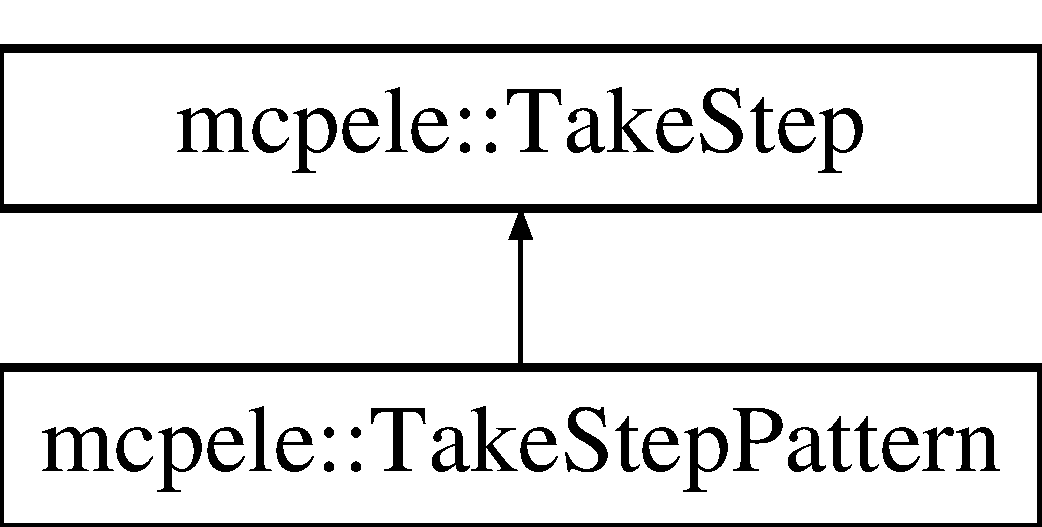
\includegraphics[height=2.000000cm]{classmcpele_1_1TakeStepPattern}
\end{center}
\end{figure}
\subsection*{\-Public \-Member \-Functions}
\begin{DoxyCompactItemize}
\item 
virtual \hyperlink{classmcpele_1_1TakeStepPattern_a574b72c67af41877b638d08b7a57e81b}{$\sim$\-Take\-Step\-Pattern} ()
\item 
void \hyperlink{classmcpele_1_1TakeStepPattern_a1bfe8206991a6aad0fdefe5ec916b31c}{add\-\_\-step} (std\-::shared\-\_\-ptr$<$ \hyperlink{classmcpele_1_1TakeStep}{\-Take\-Step} $>$ step\-\_\-input, const size\-\_\-t repetitions\-\_\-input=1)
\item 
void \hyperlink{classmcpele_1_1TakeStepPattern_a8c5ef12183c58b84b3ff5e9276ec8688}{displace} (pele\-::\-Array$<$ double $>$ \&coords, \hyperlink{classmcpele_1_1MC}{\-M\-C} $\ast$mc)
\item 
void \hyperlink{classmcpele_1_1TakeStepPattern_a6038fb5304e2a31c105fa5b537ee1b6c}{report} (pele\-::\-Array$<$ double $>$ \&old\-\_\-coords, const double old\-\_\-energy, pele\-::\-Array$<$ double $>$ \&new\-\_\-coords, const double new\-\_\-energy, const bool success, \hyperlink{classmcpele_1_1MC}{\-M\-C} $\ast$mc)
\item 
std\-::vector$<$ size\-\_\-t $>$ \hyperlink{classmcpele_1_1TakeStepPattern_a811124bbaa7ee317943d6bedb8155711}{get\-\_\-pattern} () const 
\item 
std\-::vector$<$ size\-\_\-t $>$ \hyperlink{classmcpele_1_1TakeStepPattern_ac6bf72bf5bb87c1fdd67999d88d85ed2}{get\-\_\-pattern\-\_\-direct} ()
\end{DoxyCompactItemize}


\subsection{\-Detailed \-Description}
\-Create a pattern of \-Take\-Steps to be exectuted by \hyperlink{classmcpele_1_1MC}{\-M\-C}.

\-Example -\/-\/-\/-\/-\/-\/-\/

\-To have \hyperlink{classmcpele_1_1MC}{\-M\-C} looping over a pattern consisting of 99 times step\-\_\-\-A and 1 time step\-\_\-\-B, do e.\-g.\-: auto pot = std\-::make\-\_\-shared$<$\-Some\-Potential$>$(\-Some\-Parameters); auto mc = std\-::make\-\_\-shared$<$mcpele\-::\-M\-C$>$(pot, Some\-Coordinates, Some\-Temperature); auto step\-\_\-pattern = std\-::make\-\_\-shared$<$mcpele\-::\-Take\-Step\-Pattern$>$(); auto step\-\_\-\-A = std\-::make\-\_\-shared$<$\-Some\-Take\-Step$>$(\-Some\-Parameters); auto step\-\_\-\-B = std\-::make\-\_\-shared$<$\-Some\-Other\-Take\-Step$>$(\-Some\-Other\-Parameters); step\-\_\-pattern-\/$>$add\-\_\-step(step\-\_\-\-A, 99); step\-\_\-pattern-\/$>$add\-\_\-step(step\-\_\-\-B, 1); mc-\/$>$set\-\_\-takestep(step\-\_\-pattern); mc-\/$>$run(1e6); 

\-Definition at line 26 of file take\-\_\-step\-\_\-pattern.\-h.



\subsection{\-Constructor \& \-Destructor \-Documentation}
\hypertarget{classmcpele_1_1TakeStepPattern_a574b72c67af41877b638d08b7a57e81b}{\index{mcpele\-::\-Take\-Step\-Pattern@{mcpele\-::\-Take\-Step\-Pattern}!$\sim$\-Take\-Step\-Pattern@{$\sim$\-Take\-Step\-Pattern}}
\index{$\sim$\-Take\-Step\-Pattern@{$\sim$\-Take\-Step\-Pattern}!mcpele::TakeStepPattern@{mcpele\-::\-Take\-Step\-Pattern}}
\subsubsection[{$\sim$\-Take\-Step\-Pattern}]{\setlength{\rightskip}{0pt plus 5cm}virtual {\bf mcpele\-::\-Take\-Step\-Pattern\-::$\sim$\-Take\-Step\-Pattern} (
\begin{DoxyParamCaption}
{}
\end{DoxyParamCaption}
)\hspace{0.3cm}{\ttfamily  \mbox{[}inline, virtual\mbox{]}}}}\label{classmcpele_1_1TakeStepPattern_a574b72c67af41877b638d08b7a57e81b}


\-Definition at line 30 of file take\-\_\-step\-\_\-pattern.\-h.



\subsection{\-Member \-Function \-Documentation}
\hypertarget{classmcpele_1_1TakeStepPattern_a1bfe8206991a6aad0fdefe5ec916b31c}{\index{mcpele\-::\-Take\-Step\-Pattern@{mcpele\-::\-Take\-Step\-Pattern}!add\-\_\-step@{add\-\_\-step}}
\index{add\-\_\-step@{add\-\_\-step}!mcpele::TakeStepPattern@{mcpele\-::\-Take\-Step\-Pattern}}
\subsubsection[{add\-\_\-step}]{\setlength{\rightskip}{0pt plus 5cm}void {\bf mcpele\-::\-Take\-Step\-Pattern\-::add\-\_\-step} (
\begin{DoxyParamCaption}
\item[{std\-::shared\-\_\-ptr$<$ {\bf \-Take\-Step} $>$}]{step\-\_\-input, }
\item[{const size\-\_\-t}]{repetitions\-\_\-input = {\ttfamily 1}}
\end{DoxyParamCaption}
)\hspace{0.3cm}{\ttfamily  \mbox{[}inline\mbox{]}}}}\label{classmcpele_1_1TakeStepPattern_a1bfe8206991a6aad0fdefe5ec916b31c}


\-Definition at line 31 of file take\-\_\-step\-\_\-pattern.\-h.

\hypertarget{classmcpele_1_1TakeStepPattern_a8c5ef12183c58b84b3ff5e9276ec8688}{\index{mcpele\-::\-Take\-Step\-Pattern@{mcpele\-::\-Take\-Step\-Pattern}!displace@{displace}}
\index{displace@{displace}!mcpele::TakeStepPattern@{mcpele\-::\-Take\-Step\-Pattern}}
\subsubsection[{displace}]{\setlength{\rightskip}{0pt plus 5cm}void {\bf mcpele\-::\-Take\-Step\-Pattern\-::displace} (
\begin{DoxyParamCaption}
\item[{pele\-::\-Array$<$ double $>$ \&}]{coords, }
\item[{{\bf \-M\-C} $\ast$}]{mc}
\end{DoxyParamCaption}
)\hspace{0.3cm}{\ttfamily  \mbox{[}virtual\mbox{]}}}}\label{classmcpele_1_1TakeStepPattern_a8c5ef12183c58b84b3ff5e9276ec8688}


\-Implements \hyperlink{classmcpele_1_1TakeStep_ac3032e0d99d4aa5f940ffea4a28442f5}{mcpele\-::\-Take\-Step}.



\-Definition at line 5 of file take\-\_\-step\-\_\-pattern.\-cpp.

\hypertarget{classmcpele_1_1TakeStepPattern_a811124bbaa7ee317943d6bedb8155711}{\index{mcpele\-::\-Take\-Step\-Pattern@{mcpele\-::\-Take\-Step\-Pattern}!get\-\_\-pattern@{get\-\_\-pattern}}
\index{get\-\_\-pattern@{get\-\_\-pattern}!mcpele::TakeStepPattern@{mcpele\-::\-Take\-Step\-Pattern}}
\subsubsection[{get\-\_\-pattern}]{\setlength{\rightskip}{0pt plus 5cm}std\-::vector$<$size\-\_\-t$>$ {\bf mcpele\-::\-Take\-Step\-Pattern\-::get\-\_\-pattern} (
\begin{DoxyParamCaption}
{}
\end{DoxyParamCaption}
) const\hspace{0.3cm}{\ttfamily  \mbox{[}inline\mbox{]}}}}\label{classmcpele_1_1TakeStepPattern_a811124bbaa7ee317943d6bedb8155711}


\-Definition at line 38 of file take\-\_\-step\-\_\-pattern.\-h.

\hypertarget{classmcpele_1_1TakeStepPattern_ac6bf72bf5bb87c1fdd67999d88d85ed2}{\index{mcpele\-::\-Take\-Step\-Pattern@{mcpele\-::\-Take\-Step\-Pattern}!get\-\_\-pattern\-\_\-direct@{get\-\_\-pattern\-\_\-direct}}
\index{get\-\_\-pattern\-\_\-direct@{get\-\_\-pattern\-\_\-direct}!mcpele::TakeStepPattern@{mcpele\-::\-Take\-Step\-Pattern}}
\subsubsection[{get\-\_\-pattern\-\_\-direct}]{\setlength{\rightskip}{0pt plus 5cm}std\-::vector$<$size\-\_\-t$>$ {\bf mcpele\-::\-Take\-Step\-Pattern\-::get\-\_\-pattern\-\_\-direct} (
\begin{DoxyParamCaption}
{}
\end{DoxyParamCaption}
)\hspace{0.3cm}{\ttfamily  \mbox{[}inline\mbox{]}}}}\label{classmcpele_1_1TakeStepPattern_ac6bf72bf5bb87c1fdd67999d88d85ed2}


\-Definition at line 39 of file take\-\_\-step\-\_\-pattern.\-h.

\hypertarget{classmcpele_1_1TakeStepPattern_a6038fb5304e2a31c105fa5b537ee1b6c}{\index{mcpele\-::\-Take\-Step\-Pattern@{mcpele\-::\-Take\-Step\-Pattern}!report@{report}}
\index{report@{report}!mcpele::TakeStepPattern@{mcpele\-::\-Take\-Step\-Pattern}}
\subsubsection[{report}]{\setlength{\rightskip}{0pt plus 5cm}void {\bf mcpele\-::\-Take\-Step\-Pattern\-::report} (
\begin{DoxyParamCaption}
\item[{pele\-::\-Array$<$ double $>$ \&}]{old\-\_\-coords, }
\item[{const double}]{old\-\_\-energy, }
\item[{pele\-::\-Array$<$ double $>$ \&}]{new\-\_\-coords, }
\item[{const double}]{new\-\_\-energy, }
\item[{const bool}]{success, }
\item[{{\bf \-M\-C} $\ast$}]{mc}
\end{DoxyParamCaption}
)\hspace{0.3cm}{\ttfamily  \mbox{[}inline, virtual\mbox{]}}}}\label{classmcpele_1_1TakeStepPattern_a6038fb5304e2a31c105fa5b537ee1b6c}


\-Reimplemented from \hyperlink{classmcpele_1_1TakeStep_aac4f30de62c4cbc4d9d31c7629742f64}{mcpele\-::\-Take\-Step}.



\-Definition at line 34 of file take\-\_\-step\-\_\-pattern.\-h.



\-The documentation for this class was generated from the following files\-:\begin{DoxyCompactItemize}
\item 
mcpele/\hyperlink{take__step__pattern_8h}{take\-\_\-step\-\_\-pattern.\-h}\item 
\hyperlink{take__step__pattern_8cpp}{take\-\_\-step\-\_\-pattern.\-cpp}\end{DoxyCompactItemize}

\hypertarget{classmcpele_1_1TakeStepProbabilities}{\section{mcpele\-:\-:\-Take\-Step\-Probabilities \-Class \-Reference}
\label{classmcpele_1_1TakeStepProbabilities}\index{mcpele\-::\-Take\-Step\-Probabilities@{mcpele\-::\-Take\-Step\-Probabilities}}
}


{\ttfamily \#include $<$take\-\_\-step\-\_\-probabilities.\-h$>$}

\-Inheritance diagram for mcpele\-:\-:\-Take\-Step\-Probabilities\-:\begin{figure}[H]
\begin{center}
\leavevmode
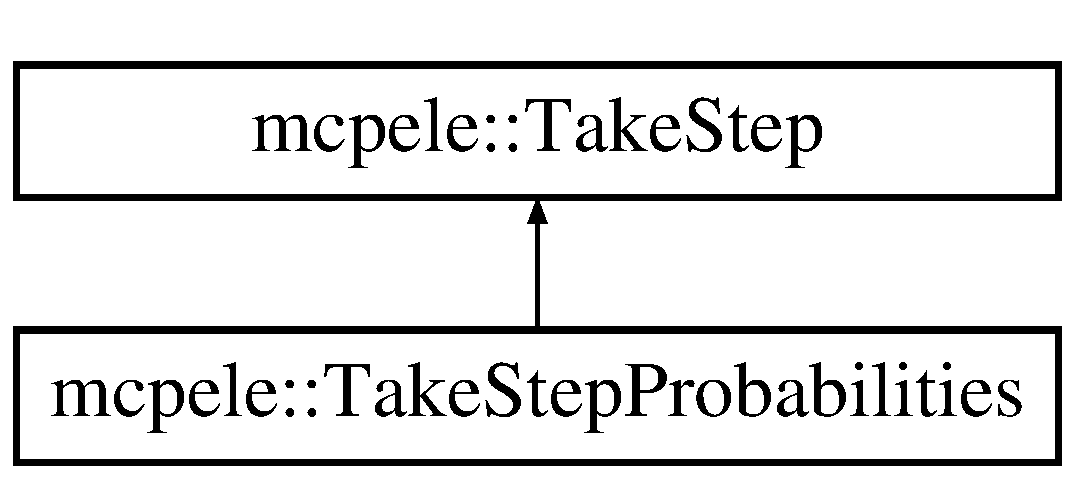
\includegraphics[height=2.000000cm]{classmcpele_1_1TakeStepProbabilities}
\end{center}
\end{figure}
\subsection*{\-Public \-Member \-Functions}
\begin{DoxyCompactItemize}
\item 
virtual \hyperlink{classmcpele_1_1TakeStepProbabilities_a6f7d0c9b37fbfb47fc4bd387472b1dac}{$\sim$\-Take\-Step\-Probabilities} ()
\item 
\hyperlink{classmcpele_1_1TakeStepProbabilities_a8079f6916d0d1052cbe41bf53610c9aa}{\-Take\-Step\-Probabilities} (const size\-\_\-t seed)
\item 
void \hyperlink{classmcpele_1_1TakeStepProbabilities_a754adeca2adcad04c43043f937fc915f}{add\-\_\-step} (std\-::shared\-\_\-ptr$<$ \hyperlink{classmcpele_1_1TakeStep}{\-Take\-Step} $>$ step\-\_\-input, const double weight\-\_\-input=1)
\item 
void \hyperlink{classmcpele_1_1TakeStepProbabilities_ae6f6a8c420950d97d463ee4cff74ad0f}{displace} (pele\-::\-Array$<$ double $>$ \&coords, \hyperlink{classmcpele_1_1MC}{\-M\-C} $\ast$mc)
\item 
void \hyperlink{classmcpele_1_1TakeStepProbabilities_a595978a5e30ba966e1f328826a8f1e68}{report} (pele\-::\-Array$<$ double $>$ \&old\-\_\-coords, const double old\-\_\-energy, pele\-::\-Array$<$ double $>$ \&new\-\_\-coords, const double new\-\_\-energy, const bool success, \hyperlink{classmcpele_1_1MC}{\-M\-C} $\ast$mc)
\item 
std\-::vector$<$ double $>$ \hyperlink{classmcpele_1_1TakeStepProbabilities_aa7e74438ac856884198539d1091b2f35}{get\-\_\-weights} () const 
\end{DoxyCompactItemize}


\subsection{\-Detailed \-Description}
\-Create a step pattern similar to \hyperlink{classmcpele_1_1TakeStepPattern}{\-Take\-Step\-Pattern}. \-However, the steps are specified together with their relative weights and exectured accoringly.

\-Reference -\/-\/-\/-\/-\/-\/-\/-\/-\/ \href{http://www.cplusplus.com/reference/random/discrete_distribution/}{\tt http\-://www.\-cplusplus.\-com/reference/random/discrete\-\_\-distribution/} 

\-Definition at line 20 of file take\-\_\-step\-\_\-probabilities.\-h.



\subsection{\-Constructor \& \-Destructor \-Documentation}
\hypertarget{classmcpele_1_1TakeStepProbabilities_a6f7d0c9b37fbfb47fc4bd387472b1dac}{\index{mcpele\-::\-Take\-Step\-Probabilities@{mcpele\-::\-Take\-Step\-Probabilities}!$\sim$\-Take\-Step\-Probabilities@{$\sim$\-Take\-Step\-Probabilities}}
\index{$\sim$\-Take\-Step\-Probabilities@{$\sim$\-Take\-Step\-Probabilities}!mcpele::TakeStepProbabilities@{mcpele\-::\-Take\-Step\-Probabilities}}
\subsubsection[{$\sim$\-Take\-Step\-Probabilities}]{\setlength{\rightskip}{0pt plus 5cm}virtual {\bf mcpele\-::\-Take\-Step\-Probabilities\-::$\sim$\-Take\-Step\-Probabilities} (
\begin{DoxyParamCaption}
{}
\end{DoxyParamCaption}
)\hspace{0.3cm}{\ttfamily  \mbox{[}inline, virtual\mbox{]}}}}\label{classmcpele_1_1TakeStepProbabilities_a6f7d0c9b37fbfb47fc4bd387472b1dac}


\-Definition at line 28 of file take\-\_\-step\-\_\-probabilities.\-h.

\hypertarget{classmcpele_1_1TakeStepProbabilities_a8079f6916d0d1052cbe41bf53610c9aa}{\index{mcpele\-::\-Take\-Step\-Probabilities@{mcpele\-::\-Take\-Step\-Probabilities}!\-Take\-Step\-Probabilities@{\-Take\-Step\-Probabilities}}
\index{\-Take\-Step\-Probabilities@{\-Take\-Step\-Probabilities}!mcpele::TakeStepProbabilities@{mcpele\-::\-Take\-Step\-Probabilities}}
\subsubsection[{\-Take\-Step\-Probabilities}]{\setlength{\rightskip}{0pt plus 5cm}{\bf mcpele\-::\-Take\-Step\-Probabilities\-::\-Take\-Step\-Probabilities} (
\begin{DoxyParamCaption}
\item[{const size\-\_\-t}]{seed}
\end{DoxyParamCaption}
)}}\label{classmcpele_1_1TakeStepProbabilities_a8079f6916d0d1052cbe41bf53610c9aa}


\-Definition at line 5 of file take\-\_\-step\-\_\-probabilities.\-cpp.



\subsection{\-Member \-Function \-Documentation}
\hypertarget{classmcpele_1_1TakeStepProbabilities_a754adeca2adcad04c43043f937fc915f}{\index{mcpele\-::\-Take\-Step\-Probabilities@{mcpele\-::\-Take\-Step\-Probabilities}!add\-\_\-step@{add\-\_\-step}}
\index{add\-\_\-step@{add\-\_\-step}!mcpele::TakeStepProbabilities@{mcpele\-::\-Take\-Step\-Probabilities}}
\subsubsection[{add\-\_\-step}]{\setlength{\rightskip}{0pt plus 5cm}void {\bf mcpele\-::\-Take\-Step\-Probabilities\-::add\-\_\-step} (
\begin{DoxyParamCaption}
\item[{std\-::shared\-\_\-ptr$<$ {\bf \-Take\-Step} $>$}]{step\-\_\-input, }
\item[{const double}]{weight\-\_\-input = {\ttfamily 1}}
\end{DoxyParamCaption}
)}}\label{classmcpele_1_1TakeStepProbabilities_a754adeca2adcad04c43043f937fc915f}


\-Definition at line 9 of file take\-\_\-step\-\_\-probabilities.\-cpp.

\hypertarget{classmcpele_1_1TakeStepProbabilities_ae6f6a8c420950d97d463ee4cff74ad0f}{\index{mcpele\-::\-Take\-Step\-Probabilities@{mcpele\-::\-Take\-Step\-Probabilities}!displace@{displace}}
\index{displace@{displace}!mcpele::TakeStepProbabilities@{mcpele\-::\-Take\-Step\-Probabilities}}
\subsubsection[{displace}]{\setlength{\rightskip}{0pt plus 5cm}void {\bf mcpele\-::\-Take\-Step\-Probabilities\-::displace} (
\begin{DoxyParamCaption}
\item[{pele\-::\-Array$<$ double $>$ \&}]{coords, }
\item[{{\bf \-M\-C} $\ast$}]{mc}
\end{DoxyParamCaption}
)\hspace{0.3cm}{\ttfamily  \mbox{[}virtual\mbox{]}}}}\label{classmcpele_1_1TakeStepProbabilities_ae6f6a8c420950d97d463ee4cff74ad0f}


\-Implements \hyperlink{classmcpele_1_1TakeStep_ac3032e0d99d4aa5f940ffea4a28442f5}{mcpele\-::\-Take\-Step}.



\-Definition at line 18 of file take\-\_\-step\-\_\-probabilities.\-cpp.

\hypertarget{classmcpele_1_1TakeStepProbabilities_aa7e74438ac856884198539d1091b2f35}{\index{mcpele\-::\-Take\-Step\-Probabilities@{mcpele\-::\-Take\-Step\-Probabilities}!get\-\_\-weights@{get\-\_\-weights}}
\index{get\-\_\-weights@{get\-\_\-weights}!mcpele::TakeStepProbabilities@{mcpele\-::\-Take\-Step\-Probabilities}}
\subsubsection[{get\-\_\-weights}]{\setlength{\rightskip}{0pt plus 5cm}std\-::vector$<$double$>$ {\bf mcpele\-::\-Take\-Step\-Probabilities\-::get\-\_\-weights} (
\begin{DoxyParamCaption}
{}
\end{DoxyParamCaption}
) const\hspace{0.3cm}{\ttfamily  \mbox{[}inline\mbox{]}}}}\label{classmcpele_1_1TakeStepProbabilities_aa7e74438ac856884198539d1091b2f35}


\-Definition at line 35 of file take\-\_\-step\-\_\-probabilities.\-h.

\hypertarget{classmcpele_1_1TakeStepProbabilities_a595978a5e30ba966e1f328826a8f1e68}{\index{mcpele\-::\-Take\-Step\-Probabilities@{mcpele\-::\-Take\-Step\-Probabilities}!report@{report}}
\index{report@{report}!mcpele::TakeStepProbabilities@{mcpele\-::\-Take\-Step\-Probabilities}}
\subsubsection[{report}]{\setlength{\rightskip}{0pt plus 5cm}void {\bf mcpele\-::\-Take\-Step\-Probabilities\-::report} (
\begin{DoxyParamCaption}
\item[{pele\-::\-Array$<$ double $>$ \&}]{old\-\_\-coords, }
\item[{const double}]{old\-\_\-energy, }
\item[{pele\-::\-Array$<$ double $>$ \&}]{new\-\_\-coords, }
\item[{const double}]{new\-\_\-energy, }
\item[{const bool}]{success, }
\item[{{\bf \-M\-C} $\ast$}]{mc}
\end{DoxyParamCaption}
)\hspace{0.3cm}{\ttfamily  \mbox{[}virtual\mbox{]}}}}\label{classmcpele_1_1TakeStepProbabilities_a595978a5e30ba966e1f328826a8f1e68}


\-Reimplemented from \hyperlink{classmcpele_1_1TakeStep_aac4f30de62c4cbc4d9d31c7629742f64}{mcpele\-::\-Take\-Step}.



\-Definition at line 27 of file take\-\_\-step\-\_\-probabilities.\-cpp.



\-The documentation for this class was generated from the following files\-:\begin{DoxyCompactItemize}
\item 
mcpele/\hyperlink{take__step__probabilities_8h}{take\-\_\-step\-\_\-probabilities.\-h}\item 
\hyperlink{take__step__probabilities_8cpp}{take\-\_\-step\-\_\-probabilities.\-cpp}\end{DoxyCompactItemize}

\chapter{\-File \-Documentation}
\hypertarget{adaptive__takestep_8cpp}{\section{adaptive\-\_\-takestep.\-cpp \-File \-Reference}
\label{adaptive__takestep_8cpp}\index{adaptive\-\_\-takestep.\-cpp@{adaptive\-\_\-takestep.\-cpp}}
}
{\ttfamily \#include \char`\"{}mcpele/adaptive\-\_\-takestep.\-h\char`\"{}}\*
\subsection*{\-Namespaces}
\begin{DoxyCompactItemize}
\item 
namespace \hyperlink{namespacemcpele}{mcpele}
\end{DoxyCompactItemize}

\hypertarget{check__spherical__container_8cpp}{\section{check\-\_\-spherical\-\_\-container.\-cpp \-File \-Reference}
\label{check__spherical__container_8cpp}\index{check\-\_\-spherical\-\_\-container.\-cpp@{check\-\_\-spherical\-\_\-container.\-cpp}}
}
{\ttfamily \#include \char`\"{}mcpele/check\-\_\-spherical\-\_\-container.\-h\char`\"{}}\*
\subsection*{\-Namespaces}
\begin{DoxyCompactItemize}
\item 
namespace \hyperlink{namespacemcpele}{mcpele}
\end{DoxyCompactItemize}

\hypertarget{energy__window__test_8cpp}{\section{energy\-\_\-window\-\_\-test.\-cpp \-File \-Reference}
\label{energy__window__test_8cpp}\index{energy\-\_\-window\-\_\-test.\-cpp@{energy\-\_\-window\-\_\-test.\-cpp}}
}
{\ttfamily \#include \char`\"{}pele/array.\-h\char`\"{}}\*
{\ttfamily \#include \char`\"{}mcpele/energy\-\_\-window\-\_\-test.\-h\char`\"{}}\*
\subsection*{\-Namespaces}
\begin{DoxyCompactItemize}
\item 
namespace \hyperlink{namespacemcpele}{mcpele}
\end{DoxyCompactItemize}

\hypertarget{gaussian__coords__displacement_8cpp}{\section{gaussian\-\_\-coords\-\_\-displacement.\-cpp \-File \-Reference}
\label{gaussian__coords__displacement_8cpp}\index{gaussian\-\_\-coords\-\_\-displacement.\-cpp@{gaussian\-\_\-coords\-\_\-displacement.\-cpp}}
}
{\ttfamily \#include \char`\"{}mcpele/gaussian\-\_\-coords\-\_\-displacement.\-h\char`\"{}}\*
\subsection*{\-Namespaces}
\begin{DoxyCompactItemize}
\item 
namespace \hyperlink{namespacemcpele}{mcpele}
\end{DoxyCompactItemize}

\hypertarget{histogram_8cpp}{\section{histogram.\-cpp \-File \-Reference}
\label{histogram_8cpp}\index{histogram.\-cpp@{histogram.\-cpp}}
}
{\ttfamily \#include \char`\"{}mcpele/histogram.\-h\char`\"{}}\*
\subsection*{\-Namespaces}
\begin{DoxyCompactItemize}
\item 
namespace \hyperlink{namespacemcpele}{mcpele}
\end{DoxyCompactItemize}

\hypertarget{lowest__eigenvalue_8cpp}{\section{lowest\-\_\-eigenvalue.\-cpp \-File \-Reference}
\label{lowest__eigenvalue_8cpp}\index{lowest\-\_\-eigenvalue.\-cpp@{lowest\-\_\-eigenvalue.\-cpp}}
}
{\ttfamily \#include $<$cmath$>$}\*
{\ttfamily \#include \char`\"{}mcpele/lowest\-\_\-eigenvalue.\-h\char`\"{}}\*
\subsection*{\-Namespaces}
\begin{DoxyCompactItemize}
\item 
namespace \hyperlink{namespacemcpele}{mcpele}
\end{DoxyCompactItemize}

\hypertarget{mc_8cpp}{\section{mc.\-cpp \-File \-Reference}
\label{mc_8cpp}\index{mc.\-cpp@{mc.\-cpp}}
}
{\ttfamily \#include \char`\"{}mcpele/mc.\-h\char`\"{}}\*
{\ttfamily \#include \char`\"{}mcpele/progress.\-h\char`\"{}}\*
\subsection*{\-Namespaces}
\begin{DoxyCompactItemize}
\item 
namespace \hyperlink{namespacemcpele}{mcpele}
\end{DoxyCompactItemize}

\hypertarget{adaptive__takestep_8h}{\section{mcpele/adaptive\-\_\-takestep.h \-File \-Reference}
\label{adaptive__takestep_8h}\index{mcpele/adaptive\-\_\-takestep.\-h@{mcpele/adaptive\-\_\-takestep.\-h}}
}
{\ttfamily \#include \char`\"{}mcpele/mc.\-h\char`\"{}}\*
\subsection*{\-Classes}
\begin{DoxyCompactItemize}
\item 
class \hyperlink{classmcpele_1_1AdaptiveTakeStep}{mcpele\-::\-Adaptive\-Take\-Step}
\end{DoxyCompactItemize}
\subsection*{\-Namespaces}
\begin{DoxyCompactItemize}
\item 
namespace \hyperlink{namespacemcpele}{mcpele}
\end{DoxyCompactItemize}

\hypertarget{check__spherical__container_8h}{\section{mcpele/check\-\_\-spherical\-\_\-container.h \-File \-Reference}
\label{check__spherical__container_8h}\index{mcpele/check\-\_\-spherical\-\_\-container.\-h@{mcpele/check\-\_\-spherical\-\_\-container.\-h}}
}
{\ttfamily \#include $<$iostream$>$}\*
{\ttfamily \#include $<$cmath$>$}\*
{\ttfamily \#include $<$algorithm$>$}\*
{\ttfamily \#include $<$random$>$}\*
{\ttfamily \#include $<$chrono$>$}\*
{\ttfamily \#include \char`\"{}pele/array.\-h\char`\"{}}\*
{\ttfamily \#include \char`\"{}pele/optimizer.\-h\char`\"{}}\*
{\ttfamily \#include \char`\"{}pele/distance.\-h\char`\"{}}\*
{\ttfamily \#include \char`\"{}mc.\-h\char`\"{}}\*
\subsection*{\-Classes}
\begin{DoxyCompactItemize}
\item 
class \hyperlink{classmcpele_1_1CheckSphericalContainer}{mcpele\-::\-Check\-Spherical\-Container}
\end{DoxyCompactItemize}
\subsection*{\-Namespaces}
\begin{DoxyCompactItemize}
\item 
namespace \hyperlink{namespacemcpele}{mcpele}
\end{DoxyCompactItemize}

\hypertarget{energy__window__test_8h}{\section{mcpele/energy\-\_\-window\-\_\-test.h \-File \-Reference}
\label{energy__window__test_8h}\index{mcpele/energy\-\_\-window\-\_\-test.\-h@{mcpele/energy\-\_\-window\-\_\-test.\-h}}
}
{\ttfamily \#include \char`\"{}pele/array.\-h\char`\"{}}\*
{\ttfamily \#include \char`\"{}mc.\-h\char`\"{}}\*
\subsection*{\-Classes}
\begin{DoxyCompactItemize}
\item 
class \hyperlink{classmcpele_1_1EnergyWindowTest}{mcpele\-::\-Energy\-Window\-Test}
\end{DoxyCompactItemize}
\subsection*{\-Namespaces}
\begin{DoxyCompactItemize}
\item 
namespace \hyperlink{namespacemcpele}{mcpele}
\end{DoxyCompactItemize}

\hypertarget{gaussian__coords__displacement_8h}{\section{mcpele/gaussian\-\_\-coords\-\_\-displacement.h \-File \-Reference}
\label{gaussian__coords__displacement_8h}\index{mcpele/gaussian\-\_\-coords\-\_\-displacement.\-h@{mcpele/gaussian\-\_\-coords\-\_\-displacement.\-h}}
}
{\ttfamily \#include $<$random$>$}\*
{\ttfamily \#include \char`\"{}mc.\-h\char`\"{}}\*
\subsection*{\-Classes}
\begin{DoxyCompactItemize}
\item 
class \hyperlink{classmcpele_1_1GaussianCoordsDisplacement}{mcpele\-::\-Gaussian\-Coords\-Displacement}
\end{DoxyCompactItemize}
\subsection*{\-Namespaces}
\begin{DoxyCompactItemize}
\item 
namespace \hyperlink{namespacemcpele}{mcpele}
\end{DoxyCompactItemize}

\hypertarget{histogram_8h}{\section{mcpele/histogram.h \-File \-Reference}
\label{histogram_8h}\index{mcpele/histogram.\-h@{mcpele/histogram.\-h}}
}
{\ttfamily \#include $<$cmath$>$}\*
{\ttfamily \#include $<$algorithm$>$}\*
{\ttfamily \#include $<$list$>$}\*
{\ttfamily \#include $<$iostream$>$}\*
{\ttfamily \#include $<$limits$>$}\*
{\ttfamily \#include \char`\"{}pele/array.\-h\char`\"{}}\*
\subsection*{\-Classes}
\begin{DoxyCompactItemize}
\item 
class \hyperlink{classmcpele_1_1Moments}{mcpele\-::\-Moments}
\item 
class \hyperlink{classmcpele_1_1Histogram}{mcpele\-::\-Histogram}
\end{DoxyCompactItemize}
\subsection*{\-Namespaces}
\begin{DoxyCompactItemize}
\item 
namespace \hyperlink{namespacemcpele}{mcpele}
\end{DoxyCompactItemize}

\hypertarget{lowest__eigenvalue_8h}{\section{mcpele/lowest\-\_\-eigenvalue.h \-File \-Reference}
\label{lowest__eigenvalue_8h}\index{mcpele/lowest\-\_\-eigenvalue.\-h@{mcpele/lowest\-\_\-eigenvalue.\-h}}
}
{\ttfamily \#include \char`\"{}pele/base\-\_\-potential.\-h\char`\"{}}\*
{\ttfamily \#include \char`\"{}pele/lbfgs.\-h\char`\"{}}\*
{\ttfamily \#include \char`\"{}pele/lowest\-\_\-eig\-\_\-potential.\-h\char`\"{}}\*
\subsection*{\-Classes}
\begin{DoxyCompactItemize}
\item 
class \hyperlink{classmcpele_1_1FindLowestEigenvalue}{mcpele\-::\-Find\-Lowest\-Eigenvalue}
\end{DoxyCompactItemize}
\subsection*{\-Namespaces}
\begin{DoxyCompactItemize}
\item 
namespace \hyperlink{namespacemcpele}{mcpele}
\end{DoxyCompactItemize}

\hypertarget{mc_8h}{\section{mcpele/mc.h \-File \-Reference}
\label{mc_8h}\index{mcpele/mc.\-h@{mcpele/mc.\-h}}
}
{\ttfamily \#include $<$cmath$>$}\*
{\ttfamily \#include $<$algorithm$>$}\*
{\ttfamily \#include $<$memory$>$}\*
{\ttfamily \#include $<$stdexcept$>$}\*
{\ttfamily \#include \char`\"{}pele/array.\-h\char`\"{}}\*
{\ttfamily \#include \char`\"{}pele/base\-\_\-potential.\-h\char`\"{}}\*
\subsection*{\-Classes}
\begin{DoxyCompactItemize}
\item 
class \hyperlink{classmcpele_1_1Action}{mcpele\-::\-Action}
\item 
class \hyperlink{classmcpele_1_1AcceptTest}{mcpele\-::\-Accept\-Test}
\item 
class \hyperlink{classmcpele_1_1ConfTest}{mcpele\-::\-Conf\-Test}
\item 
class \hyperlink{classmcpele_1_1TakeStep}{mcpele\-::\-Take\-Step}
\item 
class \hyperlink{classmcpele_1_1MC}{mcpele\-::\-M\-C}
\end{DoxyCompactItemize}
\subsection*{\-Namespaces}
\begin{DoxyCompactItemize}
\item 
namespace \hyperlink{namespacemcpele}{mcpele}
\end{DoxyCompactItemize}

\hypertarget{metropolis__test_8h}{\section{mcpele/metropolis\-\_\-test.h \-File \-Reference}
\label{metropolis__test_8h}\index{mcpele/metropolis\-\_\-test.\-h@{mcpele/metropolis\-\_\-test.\-h}}
}
{\ttfamily \#include $<$random$>$}\*
{\ttfamily \#include \char`\"{}pele/array.\-h\char`\"{}}\*
{\ttfamily \#include \char`\"{}mc.\-h\char`\"{}}\*
\subsection*{\-Classes}
\begin{DoxyCompactItemize}
\item 
class \hyperlink{classmcpele_1_1MetropolisTest}{mcpele\-::\-Metropolis\-Test}
\end{DoxyCompactItemize}
\subsection*{\-Namespaces}
\begin{DoxyCompactItemize}
\item 
namespace \hyperlink{namespacemcpele}{mcpele}
\end{DoxyCompactItemize}


\subsection{\-Detailed \-Description}
\-Metropolis acceptance criterion 

\-Definition in file \hyperlink{metropolis__test_8h_source}{metropolis\-\_\-test.\-h}.


\hypertarget{moving__average_8h}{\section{mcpele/moving\-\_\-average.h \-File \-Reference}
\label{moving__average_8h}\index{mcpele/moving\-\_\-average.\-h@{mcpele/moving\-\_\-average.\-h}}
}
{\ttfamily \#include $<$algorithm$>$}\*
{\ttfamily \#include $<$vector$>$}\*
{\ttfamily \#include \char`\"{}histogram.\-h\char`\"{}}\*
\subsection*{\-Classes}
\begin{DoxyCompactItemize}
\item 
class \hyperlink{classmcpele_1_1MovingAverageAcc}{mcpele\-::\-Moving\-Average\-Acc}
\end{DoxyCompactItemize}
\subsection*{\-Namespaces}
\begin{DoxyCompactItemize}
\item 
namespace \hyperlink{namespacemcpele}{mcpele}
\end{DoxyCompactItemize}

\hypertarget{pair__dist__histogram_8h}{\section{mcpele/pair\-\_\-dist\-\_\-histogram.h \-File \-Reference}
\label{pair__dist__histogram_8h}\index{mcpele/pair\-\_\-dist\-\_\-histogram.\-h@{mcpele/pair\-\_\-dist\-\_\-histogram.\-h}}
}
{\ttfamily \#include $<$algorithm$>$}\*
{\ttfamily \#include $<$stdexcept$>$}\*
{\ttfamily \#include $<$cmath$>$}\*
{\ttfamily \#include $<$utility$>$}\*
{\ttfamily \#include \char`\"{}pele/distance.\-h\char`\"{}}\*
{\ttfamily \#include \char`\"{}mcpele/histogram.\-h\char`\"{}}\*
\subsection*{\-Classes}
\begin{DoxyCompactItemize}
\item 
class \hyperlink{classmcpele_1_1PairDistHistogram}{mcpele\-::\-Pair\-Dist\-Histogram$<$ B\-O\-X\-D\-I\-M $>$}
\end{DoxyCompactItemize}
\subsection*{\-Namespaces}
\begin{DoxyCompactItemize}
\item 
namespace \hyperlink{namespacemcpele}{mcpele}
\end{DoxyCompactItemize}

\hypertarget{particle__pair__swap_8h}{\section{mcpele/particle\-\_\-pair\-\_\-swap.h \-File \-Reference}
\label{particle__pair__swap_8h}\index{mcpele/particle\-\_\-pair\-\_\-swap.\-h@{mcpele/particle\-\_\-pair\-\_\-swap.\-h}}
}
{\ttfamily \#include $<$random$>$}\*
{\ttfamily \#include \char`\"{}mc.\-h\char`\"{}}\*
\subsection*{\-Classes}
\begin{DoxyCompactItemize}
\item 
class \hyperlink{classmcpele_1_1ParticlePairSwap}{mcpele\-::\-Particle\-Pair\-Swap}
\end{DoxyCompactItemize}
\subsection*{\-Namespaces}
\begin{DoxyCompactItemize}
\item 
namespace \hyperlink{namespacemcpele}{mcpele}
\end{DoxyCompactItemize}

\hypertarget{pattern__manager_8h}{\section{mcpele/pattern\-\_\-manager.h \-File \-Reference}
\label{pattern__manager_8h}\index{mcpele/pattern\-\_\-manager.\-h@{mcpele/pattern\-\_\-manager.\-h}}
}
{\ttfamily \#include $<$vector$>$}\*
{\ttfamily \#include $<$utility$>$}\*
{\ttfamily \#include $<$stdexcept$>$}\*
{\ttfamily \#include \char`\"{}mc.\-h\char`\"{}}\*
\subsection*{\-Classes}
\begin{DoxyCompactItemize}
\item 
class \hyperlink{classmcpele_1_1PatternManager}{mcpele\-::\-Pattern\-Manager$<$ T $>$}
\end{DoxyCompactItemize}
\subsection*{\-Namespaces}
\begin{DoxyCompactItemize}
\item 
namespace \hyperlink{namespacemcpele}{mcpele}
\end{DoxyCompactItemize}

\hypertarget{progress_8h}{\section{mcpele/progress.h \-File \-Reference}
\label{progress_8h}\index{mcpele/progress.\-h@{mcpele/progress.\-h}}
}
{\ttfamily \#include $<$ctime$>$}\*
{\ttfamily \#include $<$utility$>$}\*
{\ttfamily \#include $<$iostream$>$}\*
{\ttfamily \#include $<$string$>$}\*
{\ttfamily \#include $<$algorithm$>$}\*
\subsection*{\-Classes}
\begin{DoxyCompactItemize}
\item 
class \hyperlink{classmcpele_1_1progress}{mcpele\-::progress}
\end{DoxyCompactItemize}
\subsection*{\-Namespaces}
\begin{DoxyCompactItemize}
\item 
namespace \hyperlink{namespacemcpele}{mcpele}
\end{DoxyCompactItemize}

\hypertarget{random__coords__displacement_8h}{\section{mcpele/random\-\_\-coords\-\_\-displacement.h \-File \-Reference}
\label{random__coords__displacement_8h}\index{mcpele/random\-\_\-coords\-\_\-displacement.\-h@{mcpele/random\-\_\-coords\-\_\-displacement.\-h}}
}
{\ttfamily \#include $<$random$>$}\*
{\ttfamily \#include \char`\"{}mc.\-h\char`\"{}}\*
\subsection*{\-Classes}
\begin{DoxyCompactItemize}
\item 
class \hyperlink{classmcpele_1_1RandomCoordsDisplacement}{mcpele\-::\-Random\-Coords\-Displacement}
\item 
class \hyperlink{classmcpele_1_1RandomCoordsDisplacementAll}{mcpele\-::\-Random\-Coords\-Displacement\-All}
\item 
class \hyperlink{classmcpele_1_1RandomCoordsDisplacementSingle}{mcpele\-::\-Random\-Coords\-Displacement\-Single}
\end{DoxyCompactItemize}
\subsection*{\-Namespaces}
\begin{DoxyCompactItemize}
\item 
namespace \hyperlink{namespacemcpele}{mcpele}
\end{DoxyCompactItemize}

\hypertarget{record__displacement__per__particle__timeseries_8h}{\section{mcpele/record\-\_\-displacement\-\_\-per\-\_\-particle\-\_\-timeseries.h \-File \-Reference}
\label{record__displacement__per__particle__timeseries_8h}\index{mcpele/record\-\_\-displacement\-\_\-per\-\_\-particle\-\_\-timeseries.\-h@{mcpele/record\-\_\-displacement\-\_\-per\-\_\-particle\-\_\-timeseries.\-h}}
}
{\ttfamily \#include \char`\"{}record\-\_\-scalar\-\_\-timeseries.\-h\char`\"{}}\*
{\ttfamily \#include \char`\"{}rsm\-\_\-displacement.\-h\char`\"{}}\*
\subsection*{\-Classes}
\begin{DoxyCompactItemize}
\item 
class \hyperlink{classmcpele_1_1RecordDisplacementPerParticleTimeseries}{mcpele\-::\-Record\-Displacement\-Per\-Particle\-Timeseries}
\end{DoxyCompactItemize}
\subsection*{\-Namespaces}
\begin{DoxyCompactItemize}
\item 
namespace \hyperlink{namespacemcpele}{mcpele}
\end{DoxyCompactItemize}

\hypertarget{record__energy__histogram_8h}{\section{mcpele/record\-\_\-energy\-\_\-histogram.h \-File \-Reference}
\label{record__energy__histogram_8h}\index{mcpele/record\-\_\-energy\-\_\-histogram.\-h@{mcpele/record\-\_\-energy\-\_\-histogram.\-h}}
}
{\ttfamily \#include \char`\"{}mc.\-h\char`\"{}}\*
{\ttfamily \#include \char`\"{}histogram.\-h\char`\"{}}\*
\subsection*{\-Classes}
\begin{DoxyCompactItemize}
\item 
class \hyperlink{classmcpele_1_1RecordEnergyHistogram}{mcpele\-::\-Record\-Energy\-Histogram}
\end{DoxyCompactItemize}
\subsection*{\-Namespaces}
\begin{DoxyCompactItemize}
\item 
namespace \hyperlink{namespacemcpele}{mcpele}
\end{DoxyCompactItemize}

\hypertarget{record__energy__timeseries_8h}{\section{mcpele/record\-\_\-energy\-\_\-timeseries.h \-File \-Reference}
\label{record__energy__timeseries_8h}\index{mcpele/record\-\_\-energy\-\_\-timeseries.\-h@{mcpele/record\-\_\-energy\-\_\-timeseries.\-h}}
}
{\ttfamily \#include \char`\"{}record\-\_\-scalar\-\_\-timeseries.\-h\char`\"{}}\*
\subsection*{\-Classes}
\begin{DoxyCompactItemize}
\item 
class \hyperlink{classmcpele_1_1RecordEnergyTimeseries}{mcpele\-::\-Record\-Energy\-Timeseries}
\end{DoxyCompactItemize}
\subsection*{\-Namespaces}
\begin{DoxyCompactItemize}
\item 
namespace \hyperlink{namespacemcpele}{mcpele}
\end{DoxyCompactItemize}

\hypertarget{record__lowest__evalue__timeseries_8h}{\section{mcpele/record\-\_\-lowest\-\_\-evalue\-\_\-timeseries.h \-File \-Reference}
\label{record__lowest__evalue__timeseries_8h}\index{mcpele/record\-\_\-lowest\-\_\-evalue\-\_\-timeseries.\-h@{mcpele/record\-\_\-lowest\-\_\-evalue\-\_\-timeseries.\-h}}
}
{\ttfamily \#include \char`\"{}record\-\_\-scalar\-\_\-timeseries.\-h\char`\"{}}\*
{\ttfamily \#include \char`\"{}lowest\-\_\-eigenvalue.\-h\char`\"{}}\*
\subsection*{\-Classes}
\begin{DoxyCompactItemize}
\item 
class \hyperlink{classmcpele_1_1RecordLowestEValueTimeseries}{mcpele\-::\-Record\-Lowest\-E\-Value\-Timeseries}
\end{DoxyCompactItemize}
\subsection*{\-Namespaces}
\begin{DoxyCompactItemize}
\item 
namespace \hyperlink{namespacemcpele}{mcpele}
\end{DoxyCompactItemize}

\hypertarget{record__pair__dist__histogram_8h}{\section{mcpele/record\-\_\-pair\-\_\-dist\-\_\-histogram.h \-File \-Reference}
\label{record__pair__dist__histogram_8h}\index{mcpele/record\-\_\-pair\-\_\-dist\-\_\-histogram.\-h@{mcpele/record\-\_\-pair\-\_\-dist\-\_\-histogram.\-h}}
}
{\ttfamily \#include \char`\"{}mc.\-h\char`\"{}}\*
{\ttfamily \#include \char`\"{}pair\-\_\-dist\-\_\-histogram.\-h\char`\"{}}\*
\subsection*{\-Classes}
\begin{DoxyCompactItemize}
\item 
class \hyperlink{classmcpele_1_1RecordPairDistHistogram}{mcpele\-::\-Record\-Pair\-Dist\-Histogram$<$ B\-O\-X\-D\-I\-M $>$}
\end{DoxyCompactItemize}
\subsection*{\-Namespaces}
\begin{DoxyCompactItemize}
\item 
namespace \hyperlink{namespacemcpele}{mcpele}
\end{DoxyCompactItemize}

\hypertarget{record__scalar__timeseries_8h}{\section{mcpele/record\-\_\-scalar\-\_\-timeseries.h \-File \-Reference}
\label{record__scalar__timeseries_8h}\index{mcpele/record\-\_\-scalar\-\_\-timeseries.\-h@{mcpele/record\-\_\-scalar\-\_\-timeseries.\-h}}
}
{\ttfamily \#include \char`\"{}mc.\-h\char`\"{}}\*
\subsection*{\-Classes}
\begin{DoxyCompactItemize}
\item 
class \hyperlink{classmcpele_1_1RecordScalarTimeseries}{mcpele\-::\-Record\-Scalar\-Timeseries}
\end{DoxyCompactItemize}
\subsection*{\-Namespaces}
\begin{DoxyCompactItemize}
\item 
namespace \hyperlink{namespacemcpele}{mcpele}
\end{DoxyCompactItemize}

\hypertarget{rsm__displacement_8h}{\section{mcpele/rsm\-\_\-displacement.h \-File \-Reference}
\label{rsm__displacement_8h}\index{mcpele/rsm\-\_\-displacement.\-h@{mcpele/rsm\-\_\-displacement.\-h}}
}
{\ttfamily \#include \char`\"{}pele/array.\-h\char`\"{}}\*
\subsection*{\-Classes}
\begin{DoxyCompactItemize}
\item 
class \hyperlink{classmcpele_1_1GetDisplacementPerParticle}{mcpele\-::\-Get\-Displacement\-Per\-Particle}
\end{DoxyCompactItemize}
\subsection*{\-Namespaces}
\begin{DoxyCompactItemize}
\item 
namespace \hyperlink{namespacemcpele}{mcpele}
\end{DoxyCompactItemize}

\hypertarget{take__step__pattern_8h}{\section{mcpele/take\-\_\-step\-\_\-pattern.h \-File \-Reference}
\label{take__step__pattern_8h}\index{mcpele/take\-\_\-step\-\_\-pattern.\-h@{mcpele/take\-\_\-step\-\_\-pattern.\-h}}
}
{\ttfamily \#include \char`\"{}pattern\-\_\-manager.\-h\char`\"{}}\*
\subsection*{\-Classes}
\begin{DoxyCompactItemize}
\item 
class \hyperlink{classmcpele_1_1TakeStepPattern}{mcpele\-::\-Take\-Step\-Pattern}
\end{DoxyCompactItemize}
\subsection*{\-Namespaces}
\begin{DoxyCompactItemize}
\item 
namespace \hyperlink{namespacemcpele}{mcpele}
\end{DoxyCompactItemize}

\hypertarget{take__step__probabilities_8h}{\section{mcpele/take\-\_\-step\-\_\-probabilities.h \-File \-Reference}
\label{take__step__probabilities_8h}\index{mcpele/take\-\_\-step\-\_\-probabilities.\-h@{mcpele/take\-\_\-step\-\_\-probabilities.\-h}}
}
{\ttfamily \#include $<$vector$>$}\*
{\ttfamily \#include $<$random$>$}\*
{\ttfamily \#include \char`\"{}mc.\-h\char`\"{}}\*
\subsection*{\-Classes}
\begin{DoxyCompactItemize}
\item 
class \hyperlink{classmcpele_1_1TakeStepProbabilities}{mcpele\-::\-Take\-Step\-Probabilities}
\end{DoxyCompactItemize}
\subsection*{\-Namespaces}
\begin{DoxyCompactItemize}
\item 
namespace \hyperlink{namespacemcpele}{mcpele}
\end{DoxyCompactItemize}

\hypertarget{metropolis__test_8cpp}{\section{metropolis\-\_\-test.\-cpp \-File \-Reference}
\label{metropolis__test_8cpp}\index{metropolis\-\_\-test.\-cpp@{metropolis\-\_\-test.\-cpp}}
}
{\ttfamily \#include \char`\"{}mcpele/metropolis\-\_\-test.\-h\char`\"{}}\*
{\ttfamily \#include $<$cmath$>$}\*
\subsection*{\-Namespaces}
\begin{DoxyCompactItemize}
\item 
namespace \hyperlink{namespacemcpele}{mcpele}
\end{DoxyCompactItemize}

\hypertarget{particle__pair__swap_8cpp}{\section{particle\-\_\-pair\-\_\-swap.\-cpp \-File \-Reference}
\label{particle__pair__swap_8cpp}\index{particle\-\_\-pair\-\_\-swap.\-cpp@{particle\-\_\-pair\-\_\-swap.\-cpp}}
}
{\ttfamily \#include \char`\"{}mcpele/particle\-\_\-pair\-\_\-swap.\-h\char`\"{}}\*
\subsection*{\-Namespaces}
\begin{DoxyCompactItemize}
\item 
namespace \hyperlink{namespacemcpele}{mcpele}
\end{DoxyCompactItemize}

\hypertarget{random__coords__displacement_8cpp}{\section{random\-\_\-coords\-\_\-displacement.\-cpp \-File \-Reference}
\label{random__coords__displacement_8cpp}\index{random\-\_\-coords\-\_\-displacement.\-cpp@{random\-\_\-coords\-\_\-displacement.\-cpp}}
}
{\ttfamily \#include \char`\"{}mcpele/random\-\_\-coords\-\_\-displacement.\-h\char`\"{}}\*
\subsection*{\-Namespaces}
\begin{DoxyCompactItemize}
\item 
namespace \hyperlink{namespacemcpele}{mcpele}
\end{DoxyCompactItemize}

\hypertarget{record__energy__histogram_8cpp}{\section{record\-\_\-energy\-\_\-histogram.\-cpp \-File \-Reference}
\label{record__energy__histogram_8cpp}\index{record\-\_\-energy\-\_\-histogram.\-cpp@{record\-\_\-energy\-\_\-histogram.\-cpp}}
}
{\ttfamily \#include \char`\"{}mcpele/record\-\_\-energy\-\_\-histogram.\-h\char`\"{}}\*
\subsection*{\-Namespaces}
\begin{DoxyCompactItemize}
\item 
namespace \hyperlink{namespacemcpele}{mcpele}
\end{DoxyCompactItemize}

\hypertarget{record__scalar__timeseries_8cpp}{\section{record\-\_\-scalar\-\_\-timeseries.\-cpp \-File \-Reference}
\label{record__scalar__timeseries_8cpp}\index{record\-\_\-scalar\-\_\-timeseries.\-cpp@{record\-\_\-scalar\-\_\-timeseries.\-cpp}}
}
{\ttfamily \#include \char`\"{}mcpele/record\-\_\-scalar\-\_\-timeseries.\-h\char`\"{}}\*
{\ttfamily \#include \char`\"{}mcpele/moving\-\_\-average.\-h\char`\"{}}\*
\subsection*{\-Namespaces}
\begin{DoxyCompactItemize}
\item 
namespace \hyperlink{namespacemcpele}{mcpele}
\end{DoxyCompactItemize}

\hypertarget{rsm__displacement_8cpp}{\section{rsm\-\_\-displacement.\-cpp \-File \-Reference}
\label{rsm__displacement_8cpp}\index{rsm\-\_\-displacement.\-cpp@{rsm\-\_\-displacement.\-cpp}}
}
{\ttfamily \#include $<$cmath$>$}\*
{\ttfamily \#include $<$stdexcept$>$}\*
{\ttfamily \#include \char`\"{}mcpele/histogram.\-h\char`\"{}}\*
{\ttfamily \#include \char`\"{}mcpele/rsm\-\_\-displacement.\-h\char`\"{}}\*
\subsection*{\-Namespaces}
\begin{DoxyCompactItemize}
\item 
namespace \hyperlink{namespacemcpele}{mcpele}
\end{DoxyCompactItemize}

\hypertarget{take__step__pattern_8cpp}{\section{take\-\_\-step\-\_\-pattern.\-cpp \-File \-Reference}
\label{take__step__pattern_8cpp}\index{take\-\_\-step\-\_\-pattern.\-cpp@{take\-\_\-step\-\_\-pattern.\-cpp}}
}
{\ttfamily \#include \char`\"{}mcpele/take\-\_\-step\-\_\-pattern.\-h\char`\"{}}\*
\subsection*{\-Namespaces}
\begin{DoxyCompactItemize}
\item 
namespace \hyperlink{namespacemcpele}{mcpele}
\end{DoxyCompactItemize}

\hypertarget{take__step__probabilities_8cpp}{\section{take\-\_\-step\-\_\-probabilities.\-cpp \-File \-Reference}
\label{take__step__probabilities_8cpp}\index{take\-\_\-step\-\_\-probabilities.\-cpp@{take\-\_\-step\-\_\-probabilities.\-cpp}}
}
{\ttfamily \#include \char`\"{}mcpele/take\-\_\-step\-\_\-probabilities.\-h\char`\"{}}\*
\subsection*{\-Namespaces}
\begin{DoxyCompactItemize}
\item 
namespace \hyperlink{namespacemcpele}{mcpele}
\end{DoxyCompactItemize}

\printindex
\end{document}
